\documentclass[a4paper]{article}
\usepackage[T1]{fontenc}			% \chapter package
\usepackage[english]{babel}
\usepackage[english]{isodate}  		% date format
\usepackage{graphicx}				% manage images
\usepackage{subcaption}             % manage subfigures
\usepackage{amsfonts}
\usepackage{booktabs}				% high quality tables
\usepackage{amsmath}				% math package
\usepackage{amssymb}				% another math package (e.g. \nexists)
\usepackage{bm}                     % bold math symbols
\usepackage{mathtools}				% emphasize equations
\usepackage{amsthm}					% better theorems
\usepackage{enumitem}				% manage list
\usepackage{pifont}					% nice itemize
\usepackage{cancel}					% cancel math equations
\usepackage{caption}				% custom caption
\usepackage[]{mdframed}				% box text
\usepackage{multirow}				% more lines in a table
\usepackage[x11names]{xcolor}		% RGB color
\usepackage[many]{tcolorbox}		% colorful box
\usepackage{listings}               % use to writing code
\usepackage{qrcode}                 % use for qr-codes
\usepackage{fontawesome5}           % use for icons
\usepackage{ragged2e}               % use for \flushleft command
\usepackage{cite}                   % references
\usepackage{imakeidx}               % index
\usepackage{fancyhdr}               % extensive facilities, both for constructing headers and footers 
\usepackage{wrapfig}                % allows figures or tables to have text wrapped around them
\makeindex[program=makeindex, columns=1,
           title=Index, 
           intoc,
           options={-s index-style.ist}]
\usepackage{multicol}               % multi-column itemize
\usepackage{soul}                   % highlight text (as a highlighter)
\usepackage{tikz}
\usetikzlibrary{arrows.meta, positioning}

%\pdfcompresslevel=0
%\pdfobjcompresslevel=0

\definecolor{codegreen}{rgb}{0,0.6,0}
\definecolor{codegray}{rgb}{0.5,0.5,0.5}
\definecolor{codepurple}{rgb}{0.58,0,0.82}
\definecolor{backcolour}{rgb}{255,255,255}
\lstdefinestyle{mystyle}{
    backgroundcolor=\color{backcolour},   
	commentstyle=\color{codegreen},
	keywordstyle=\color{magenta},
	numberstyle=\tiny\color{codegray},
	stringstyle=\color{codepurple},
	basicstyle=\ttfamily\footnotesize,
	breakatwhitespace=false,         
	breaklines=true,                 
	captionpos=b,                    
	keepspaces=true,                 
	numbers=left,                    
	numbersep=5pt,                  
	showspaces=false,                
	showstringspaces=false,
	showtabs=false,                  
	tabsize=2,
    mathescape,
    frame=lines
}

\lstdefinelanguage{JavaScript}{
	keywords={typeof, new, true, false, catch, function, return, null, catch, switch, var, if, in, while, do, else, case, break, reduce, map},
	keywordstyle=\color{blue}\bfseries,
	ndkeywords={class, export, boolean, throw, implements, import, this, const},
	ndkeywordstyle=\color{darkgray}\bfseries,
	identifierstyle=\color{black},
	sensitive=false,
	comment=[l]{//},
	morecomment=[s]{/*}{*/},
	commentstyle=\color{codegreen}\ttfamily,
	stringstyle=\color{red}\ttfamily,
	morestring=[b]',
	morestring=[b]"
}

\lstset{
	language=JavaScript,
	backgroundcolor=\color{lightgray},
	extendedchars=true,
	basicstyle=\footnotesize\ttfamily,
	showstringspaces=false,
	showspaces=false,
	numbers=left,
	numberstyle=\footnotesize,
	numbersep=9pt,
	tabsize=2,
	breaklines=true,
	showtabs=false,
	captionpos=b
}

\lstset{style=mystyle}


% thanks Mico: https://tex.stackexchange.com/a/60218/312896
\makeatletter
\renewcommand\paragraph{\@startsection{paragraph}{4}{\z@}%
            {-2.5ex\@plus -1ex \@minus -.25ex}%
            {1.25ex \@plus .25ex}%
            {\normalfont\normalsize\bfseries}}
\makeatother
\setcounter{secnumdepth}{4} % how many sectioning levels to assign numbers to
\setcounter{tocdepth}{4}    % how many sectioning levels to show in ToC


% draw a frame around given text
\newcommand{\framedtext}[1]{%
	\par%
	\noindent\fbox{%
		\parbox{\dimexpr\linewidth-2\fboxsep-2\fboxrule}{#1}%
	}%
}


% table of content links
\usepackage{xcolor}
\usepackage[linkcolor=black, citecolor=blue, urlcolor=cyan]{hyperref} % hypertexnames=false
\hypersetup{
	colorlinks=true
}


\newtheorem{theorem}{\textcolor{Red3}{\underline{Theorem}}}
\newtheorem{lemma}[theorem]{\textcolor{Red3}{\underline{Lemma}}}
\renewcommand{\qedsymbol}{QED}
\newcommand{\dquotes}[1]{``#1''}
\newcommand{\longline}{\noindent\rule{\textwidth}{0.4pt}}
\newcommand{\circledtext}[1]{\raisebox{.5pt}{\textcircled{\raisebox{-.9pt}{#1}}}}
\newcommand{\important}[1]{\textcolor{red}{\textbf{#1}}}
\newcommand{\definition}[1]{\textcolor{Red3}{\textbf{#1}}\index{#1}}
\newcommand{\blackdefinition}[1]{\textbf{#1}\index{#1}}
\newcommand{\definitionWithSpecificIndex}[3]{\textcolor{Red3}{\textbf{#1}}\index{#2}\index{#3}}
\newcommand{\example}[1]{\textcolor{Green4}{\textbf{#1}}}
\newcommand{\highspace}{\vspace{1.2em}\noindent}
\renewcommand{\lstlistingname}{Algorithm}
\renewcommand{\lstlistlistingname}{Algorithms}
\newcommand{\hqlabel}[2]{\label{#1}\hypertarget{#1}{#2}}
\newcommand{\hqpageref}[1]{\hyperlink{#1}{\hypergetpageref{#1}}}
\newcommand{\version}{v1.0.0-dev}
% fontawesome5 macro:
% I never remember every icon, so I use custom commands to do this
\newcommand{\speedIcon}{tachometer-alt}

% development:
\includeonly{
    sections/heterogeneous-computing-dsls-and-hls/introduction-to-heterogeneous-computing,
    sections/heterogeneous-computing-dsls-and-hls/heterogeneous-parallel-programming,
    sections/heterogeneous-computing-dsls-and-hls/dsls-and-halide,
    sections/heterogeneous-computing-dsls-and-hls/scheduling-and-performance-optimization-in-halide,
    sections/heterogeneous-computing-dsls-and-hls/introduction-to-hls,
    sections/heterogeneous-computing-dsls-and-hls/hls-workflow
}

\begin{document}
    \newcounter{definition}[section]
    \newcounter{example}[section]
    \newcounter{exercise}[section]
    
    \newtcolorbox[use counter = definition]{definitionbox}[1][]{%
        breakable,
        enhanced,
        colback=red!5!white,
        colframe=red!75!black,
        fonttitle=\bfseries,
        title={Definition \thetcbcounter#1} %
    }

    \newtcolorbox[]{pthreadbox}[1][]{%
        breakable,
        enhanced,
        colback=Red3!5!white,
        colframe=Red3!75!black,
        fonttitle=\bfseries,
        title={pthread API#1} %
    }

    \newtcolorbox[]{openmpbox}[1][]{%
        breakable,
        enhanced,
        colback=Red3!5!white,
        colframe=Red3!75!black,
        fonttitle=\bfseries,
        title={OpenMP#1} %
    }

    \newtcolorbox[use counter = exercise]{exercisebox}[1][]{%
        breakable,
        enhanced,
        colback=Red3!5!white,
        colframe=Red3!75!black,
        fonttitle=\bfseries,
        title={Exercise \thetcbcounter#1} %
    }
    
    \newtcolorbox[use counter = example]{examplebox}[1][]{%
        breakable,
        enhanced,
        colback=Green4!5!white,
        colframe=Green4!75!black,
        fonttitle=\bfseries,
        title={Example \thetcbcounter#1} %
    }

    \newtcolorbox[]{remarkbox}[1][]{%
        breakable,
        enhanced,
        colback=DarkOrange3!5!white,
        colframe=DarkOrange3!75!black,
        fonttitle=\bfseries,
        title={Remark#1} %
    }

    %%%%%%%%%%%%%%%
    % Notes cover %
    %%%%%%%%%%%%%%%
    \author{260236}
\title{Quantum Computing - Notes - \version}
\date{\printdayoff\today}
\maketitle

    %%%%%%%%%%%-dev
	\section*{Preface}

Every theory section in these notes has been taken from two sources:
\begin{itemize}
    \item Ian Goodfellow and Yoshua Bengio and Aaron Courville, \href{https://www.deeplearningbook.org/}{Deep Learning}, MIT Press. \cite{Goodfellow-et-al-2016}
    \item Course slides.\cite{course-slides-polimi}
\end{itemize}
About:
\begin{itemize}
    \item[\faIcon{github}] \href{https://github.com/PoliMI-HPC-E-notes-projects-AndreVale69/HPC-E-PoliMI-university-notes}{GitHub repository}
    \begin{center}
        \qrcode{https://github.com/PoliMI-HPC-E-notes-projects-AndreVale69/HPC-E-PoliMI-university-notes}
    \end{center}
\end{itemize}
These notes are an unofficial resource and shouldn't replace the course material or any other book on artificial neural networks and deep learning. It is not made for commercial purposes. I've made the following notes to help me improve my knowledge and maybe it can be helpful for everyone.

As I have highlighted, a student should choose the teacher's material or a book on the topic. These notes can only be a helpful material.

\highspace
During the Artificial Neural Networks and Deep Learning course, me and my other three colleagues Alberto Ondei, \href{https://it.linkedin.com/in/javedabdullah}{Abdullah Javed} and \href{https://www.hpc.cineca.it/staff/barbari-filippo/}{Filippo Barbari}, we created two projects:
\begin{itemize}
    \item[\faIcon{github}] \href{https://github.com/PoliMI-HPC-E-notes-projects-AndreVale69/AN2DL-Challenge-1}{Time Series Classification}. Deep Neural Netowrk (TCN $+$ BiLSTM with Attention) model on multivariate time-series classification.
    \begin{center}
        \qrcode{https://github.com/PoliMI-HPC-E-notes-projects-AndreVale69/AN2DL-Challenge-1}
    \end{center}
    \item[\faIcon{github}] \href{https://github.com/PoliMI-HPC-E-notes-projects-AndreVale69/AN2DL-Challenge-2}{Image Classification}. Histopathology image classification to predict molecular subtypes.
    \begin{center}
        \qrcode{https://github.com/PoliMI-HPC-E-notes-projects-AndreVale69/AN2DL-Challenge-2}
    \end{center}
\end{itemize}

    %%%%%%%%%%%%%%%%%%%%%
    % Table of contents %
    %%%%%%%%%%%%%%%%%%%%%
    \tableofcontents
    \newpage

    %%%%%%%%%%%%%%%%%%%
    % Fancy pagestyle %
    %%%%%%%%%%%%%%%%%%%
    \pagestyle{fancy}
    \fancyhead{} % clear all header fields
    \fancyhead[R]{\nouppercase{\leftmark\hfill\rightmark}}

    %%%%%%%%
    % PRAM %
    %%%%%%%%
    \section{PRAM}

\subsection{Prerequisites}

Before we introduce the PRAM model, we need to cover some useful topics.
\begin{itemize}
    \item A \definition{Machine Model} describes a \dquotes{machine}. It gives a value to the operations on the machine. It is necessary because: it makes it easy to deal with algorithms; it achieves complexity bounds; it analyses maximum parallelism.

    \item A \definition{Random Access Machine (RAM)} is a model of computation that describes an abstract machine in the general class of register machines. Some features are:
    \begin{itemize}
        \item \textbf{Unbounded} number of local memory cells;
        \item Each memory cell can hold an integer of \textbf{unbounded} size;
        \item Instruction set includes simple operations, data operations, comparator, branches;
        \item All operations take \textbf{unit time};
        \item The definition of \textbf{time complexity} is the number of instructions executed;
        \item The definition of \textbf{space complexity} is the number of memory cells used.
    \end{itemize}
\end{itemize} % and definition
    \subsection{How it works}

The multigrid method is divided into \textbf{seven parts} that make the MG method work.
\begin{enumerate}
    \item \textbf{Coarse Grids} (page \pageref{subsubsection: Coarse Grids})
    \item \textbf{Correction} (page \pageref{subsubsection: Correction})
    \item \textbf{Interpolation Operator} (page \pageref{subsubsection: Interpolation Operator})
    \item \textbf{Restriction Operator} (page \pageref{subsubsection: Restriction Operator})
    \item \textbf{Two-Grid Scheme} (page \pageref{subsubsection: Two-Grid Scheme})
    \item \textbf{V-Cycle Scheme} (page \pageref{subsubsection: V-Cycle Scheme})
\end{enumerate}

\noindent
These elements \textbf{work together to handle errors at different scales}, making the method \textbf{highly effective for solving large and complex systems} of linear equations.

\highspace
Note that this \textbf{is \underline{not} an algorithm!} We can think of the MG method as a toolbox filled with powerful tools, each designed to address different aspects of solving complex problems efficiently.

\begin{flushleft}
    \textcolor{Green3}{\faIcon{square-root-alt} \textbf{Notation used in MG methods}}
\end{flushleft}
We will use the subscript $h$ to indicate the Grid Spacing. The variable $h$ represents the \textbf{distance between two successive grid points on the fine grid}. For example, if the domain is divided into $N$ intervals, the grid spacing $h$ is typically $\frac{1}{N}$.
\begin{itemize}
    \item \textbf{Residual} $\mathbf{r}_{h}$ represents the residual calculated on the fine grid with spacing $h$. It's the difference between the current solution and the exact solution on this grid.

    \item \textbf{Solution} $\mathbf{x}_{h}$ indicates the approximate solution on the fine grid. This solution is updated iteratively using the Multigrid method.
    
    \item \textbf{Operator} $A_{h}$ is the matrix or operator that represents the system of equations on the fine grid. This operator acts on the solution $\mathbf{x}_{h}$.
    
    \item \textbf{Right-Hand Side} $\mathbf{b}_{h}$ is the right-hand side vector of the system of equations on the fine grid. It's what the solution $\mathbf{x}_{h}$ should ideally satisfy when acted upon by $A_{h}$.
    
    \item \textbf{Error on the Fine Grid} $\mathbf{e}_{h}$ is the error estimate or correction term calculated on the fine grid. It represents the difference between the true solution and the current approximate solution on the fine grid with spacing $h$.
\end{itemize}
What's more, \textbf{if we move to a coarser grid}, the grid spacing will be greater, indicated by $2h$ or even $4h$ if we make a significant jump to a coarser level.
    \subsection{MVM algorithm}

The \definition{Matrix-Vector Multiply (MVM) algorithm} consists of four steps:
\begin{enumerate}
    \item \textbf{Concurrent read of vector} $X\left(1 : n\right)$ (transfer $N$ elements);

    \item \textbf{Simultaneous reads of different sections of the general matrix} $A$ (transfer $\dfrac{n^{2}}{p}$ elements to each processor);

    \item \textbf{Compute} $\dfrac{n^{2}}{p}$ operations per processor;

    \item \textbf{Simultaneous writes} (transfer $\dfrac{n}{p}$ elements from each processor).
\end{enumerate}
Let $i$ be the processor index, so the MVM algorithm is simply written as:
\begin{lstlisting}[mathescape=true, caption={Matrix-Vector Multiply (MVM)}]
GLOBAL READ (Z $\leftarrow$ X)
GLOBAL READ (B $\leftarrow A_{i}$)
COMPUTE (W := BZ)
GLOBAL WRITE (W $\rightarrow y _{i}$)
\end{lstlisting}

\highspace
\begin{figure}[!htp]
    \centering
    \includegraphics[width=.7\textwidth]{img/mvm-1.pdf}
    \caption{Example of MVM algorithm.}
\end{figure}

\newpage

\noindent
The performance of the MVM algorithm is as follows:
\begin{itemize}
    \item The \textbf{time to solve} a problem of size $n^{2}$ is equal to the big $O$ of the squared size of the problem as input divided by the number of processors available:
    \begin{equation*}
        T_{p}\left(n^{2}\right) = O\left(\dfrac{n^{2}}{p}\right)
    \end{equation*}
    
    \item The \textbf{cost} is equal to the number of processors and the time it takes to solve the problem. So it is quite trivial:
    \begin{equation*}
        C = O\left(\cancel{P} \cdot \dfrac{n^{2}}{\cancel{p}}\right) = O\left(n^{2}\right)
    \end{equation*}

    \item The \textbf{work} is equal to the cost, and the \textbf{linear power} $P$ is equal to the ratio of work and time to solve the problem on $p$ processors:
    \begin{equation*}
        W = C \hspace{2em} \dfrac{W}{T_{p}} = P
    \end{equation*}

    \item The \textbf{perfect efficiency} is equal to:
    \begin{equation*}
        E_{p} = \dfrac{T_{1}}{pT_{p}} = \dfrac{n^{2}}{p\frac{n^{2}}{p}} = 1
    \end{equation*}
\end{itemize}
    \subsection{SPMD sum}

The \definition{Single Program Multiple Data (SPMD)} is a term that has been used to \textbf{describe computational models} for exploiting parallelism, where \textbf{multiple processors work together to execute a program to get results faster}.

\highspace
In this section, we will see an SPMD approach on a Parallel Random Access Machine (PRAM). We will introduce one of the most common and simple mathematical operations: the sum.

\highspace
The following pseudocode takes as \textbf{input an array} of size $n = 2^{k}$. In this case, $n$ is a power of 2 because it ensures that the array can be evenly divided at each step of the computation. The value $k$ is the number of iterations or levels of the summation process.
\begin{lstlisting}[mathescape=true, caption={Single Program Multiple Data (SPMD) sum}]
BEGIN
    GLOBAL READ (A $\leftarrow$ A(I))
    GLOBAL WRITE (A $\rightarrow$ B(I))
    FOR H = 1 : K
        IF $i \le n \div 2^{h}$ THEN BEGIN
            GLOBAL READ (X $\leftarrow$ B(2$i$ - 1))
            GLOBAL READ (Y $\leftarrow$ B(2$i$))
            Z := X + Y
            GLOBAL WRITE (Z $\rightarrow$ B($i$))
        END
    IF I = 1 THEN
        GLOBAL WRITE (Z $\rightarrow$ S)
END
\end{lstlisting}
\begin{itemize}
    \item First, read the entire input array \texttt{A} and copy the read data to another array \texttt{B}.
    
    \item Loop over \texttt{h} (\texttt{1 to k}). In each iteration, for each index $i$ less than or equal to $n \div 2^{h}$, read values from array \texttt{B} at positions $2i-1$ and $2i$; sum these values (and store the result in \texttt{Z}) and store the result (\texttt{Z}) back into \texttt{B($i$)}.
    
    \item Once all iterations are complete, the final sum is stored in a variable \texttt{S}.
\end{itemize}
For example, if $n = 8$, then $k$ would be 3, meaning that the algorithm will run for 3 iterations to sum all the elements in parallel.
\begin{table}[!htp]
    \centering
    \begin{tabular}{@{} c c c @{}}
        \toprule
        $h$ & $i$ & adding \\
        \midrule
        \multirow{4}{*}{1} & 1 & 1,2 \\
          & 2 & 3,4 \\
          & 3 & 5,6 \\
          & 4 & 7,8 \\
        \cmidrule{1-3}
        \multirow{2}{*}{2} & 1 & 1,2 \\
          & 2 & 3,4 \\
        \cmidrule{1-3}
        3 & 1 & 1,2 \\
        \bottomrule
    \end{tabular}
\end{table}

\newpage

\begin{figure}[!htp]
    \centering
    \includegraphics[width=\textwidth]{img/SPDM-sum-1.jpg}
    \caption{Computation of the sum of eight elements on a PRAM with eight processors. Each internal node represents a sum operation. The specific processor executing the operation is indicated below each node.}
    \label{fig: SPDM-sum-1}
\end{figure}

\begin{flushleft}
    \textcolor{Green3}{\faIcon{tachometer-alt} \textbf{Performance of sum}}
\end{flushleft}
When the size of the array is equal to the number of processors ($N = P$), the \textbf{speedup and efficiency decrease}:
\begin{itemize}
    \item $T^{*}\left(N\right) = T_{1}\left(N\right) = N$
    \item $T_{N=P}\left(N\right) = 2 + \log N$
    \item $\mathrm{SU}_{P} = \dfrac{N}{2+\log N}$
    \item $T^{*}\left(N\right) = P \cdot \left(2 + \log N\right) \approx N \log N$
    \item $E_{p} = \dfrac{T_{1}}{pT_{p}} = \dfrac{N}{N \log N} = \dfrac{1}{\log N}$
\end{itemize}
\begin{figure}[!htp]
    \centering
    \begin{subfigure}[h]{0.45\linewidth}
        \includegraphics[width=\linewidth]{img/SPDM-sum-2.png}
    \end{subfigure}
    \hfill
    \begin{subfigure}[h]{0.45\linewidth}
        \includegraphics[width=\linewidth]{img/SPDM-sum-3.png}
    \end{subfigure}
\end{figure}

\newpage

\noindent
If the size of the array is much larger than the number of processors ($N \gg P$), the \textbf{speedup and power are linear}, the \textbf{cost is fixed} and the \textbf{efficiency is maximum (equal to 1)}:
\begin{itemize}
    \item $T^{*}\left(N\right) = T_{1}\left(N\right) = N$
    \item $T_{p}\left(N\right) = \dfrac{N}{p} + \log p$
    \item $\mathrm{SU}_{P} = \dfrac{N}{\frac{N}{p}+\log p} \approx P$
    \item $\text{COST} = p\left(\dfrac{N}{p} + \log p\right) \approx N$
    \item $\text{WORK} = N + P \approx N$
    \item $E_{p} = \dfrac{T_{1}}{pT_{p}} = \dfrac{N}{p\left(\frac{N}{p} + \log p\right)} \approx 1$
\end{itemize}
\begin{figure}[!htp]
    \centering
    \includegraphics[width=.5\linewidth]{img/SPDM-sum-4.png}
    \caption*{$n = 1'000'000$}
\end{figure}

\begin{examplebox}
    Refer to Figure \ref{fig: SPDM-sum-1} (page \pageref{fig: SPDM-sum-1}), the performance metrics are:
    \begin{itemize}
        \item $T_{8} = 5$
        \item $C = 8 \cdot 5 = 40$ (could do 40 steps)
        \item $W = 2n = 16$ (16 on 40, wasted 24)
        \item $E_{p} = \dfrac{2}{\log n} = \dfrac{2}{3} = 0.67$
        \item $\dfrac{W}{C} = \dfrac{16}{40} = 0.4$
    \end{itemize}
\end{examplebox}

\noindent
There is also the \definition{Prefix Sum}, which takes \textbf{advantage of idle processors in the sum}. It computes all prefix sums:
\begin{equation*}
    S_{i} = \displaystyle\sum_{1}^{i} a_{j} \hspace{2em} a_{1}, \hspace{1em} a_{1}+a_{2}, \hspace{1em} a_{1}+a_{2}+a_{3}
\end{equation*}
\begin{figure}[!htp]
    \centering
    \includegraphics[width=.7\textwidth]{img/prefix-sum-1.pdf}
    \caption{Prefix sum.}
\end{figure}
    \subsection{MM algorithm}

The \definition{Matrix Multiply (MM) algorithm} consists of three steps:
\begin{enumerate}
    \item \textbf{Compute the two matrices} $A_{i,l}$ and $B_{l,j}$, so use the concurrent read.
    \item Make the \textbf{sum}.
    \item \textbf{Store} the result using exclusive write.
\end{enumerate}
\begin{lstlisting}[mathescape=true, caption={Matrix Multiply (MM)}]
BEGIN
    $T_{i,j,l}$ = $A_{i,l} B_{l,j}$
    FOR = H = 1 : K
        IF $l \le n \div 2^{h}$ THEN
            $T_{i,j,l}$ = $T_{i,j,2l-1}$ + $T_{i,j,2l}$
    IF $l = 1$ THEN
        $C_{i,j}$ = $T_{i,j,1}$
END
\end{lstlisting}
\begin{flushleft}
    \textcolor{Green3}{\faIcon{tachometer-alt} \textbf{Performance of MM}}
\end{flushleft}
\begin{itemize}
    \item $T_{1} = n^{3}$
    \item $T_{p = n^{3}} = \log n$
    \item $\mathrm{SU} = \dfrac{n^{3}}{\log n}$
    \item $\text{Cost} = n^{3} \log n$
    \item $E_{p} = \dfrac{T_{1}}{pT_{p}} = \dfrac{1}{\log n}$
\end{itemize}
\begin{figure}[!htp]
    \centering
    \includegraphics[width=.6\textwidth]{img/mm-1.png}
\end{figure}
    \subsection{PRAM variants and Lemmas}

The PRAM model presented here is one of the most commonly used. However, there are other important variants:
\begin{itemize}
    \item PRAM model with a \textbf{limited number of shared memory cells} (small memory PRAM). If the input data set exceeds the capacity of the shared memory, the I/O values can be evenly distributed among the processors.
    
    \item PRAM model with \textbf{limited number of processors} (small PRAM). If the number of execution threads is higher, processors can interleave multiple threads.

    \item PRAM model with \textbf{limited size of one machine word}.
    
    \item PRAM model with \textbf{access conflicts handling}. These are restrictions on simultaneous access to shared memory cells.
\end{itemize}

\begin{lemma}
    Assume $P' < P$ and same size of shared memory. Any problem that can be solved for a $P$ processor PRAM in $T$ steps can be solved in a $P'$ processor PRAM in:
    \begin{equation}
        T' = O\left(\dfrac{TP}{P'}\right)
    \end{equation}
\end{lemma}
\begin{proof}
    Partition $P$ is simulated processors into $P'$ groups of size $\frac{P}{P'}$ each. Associate each of the $P'$ simulating processors with one of these groups. Each of the simulating processors simulates one step of its group of processors by:
    \begin{itemize}
        \item Executing all their read and local computation substeps first;
        \item Executing their write substeps then.
    \end{itemize}
\end{proof}

\highspace
\begin{lemma}
    Assume $M' < M$. Any problem that can be solved for a $P$ processor and $M$-cell PRAM in $T$ steps can be solved on a $\max\left(P, M'\right)$-processors $M'$-cell PRAM in $O\left(\dfrac{TM}{M'}\right)$ steps.
\end{lemma}
\begin{proof}
    Partition $M$ simulated shared memory cells into $M'$ continuous segments $S$, of size $\frac{M}{M'}$ each. Each simulating processor $P_{I}'$ ($1 \le I \le P$), will simulate processor $P_{I}$ of the original PRAM. Each simulating processor $P_{I}'$ ($1 \le I \le M'$), stores the initial contents of $S_{I}$ into its local memory and will use $M'\left[I\right]$ as an auxiliary memory cell for simulation of accesses to cell of $S_{I}$.

    \noindent
    Simulation of one original read operation:
    \begin{lstlisting}[mathescape=true]
EACH $P_{I}'$ $\left(I = 1, \dots, \max\left(P, M'\right)\right)$ REPEATS FOR K = 1, ..., $\frac{M}{M'}$
    WRITE THE VALUE OF THE K-TH CELL OF $S_{I}$ INTO $M'\left[I\right]$ $\left(I = 1, \dots, M'\right)$
    READ THE VALUE WHICH THE SIMULATED PROCESSOR $P_{I}$ $\left(I = 1, \dots, P\right)$ WOULD READ IN THIS SIMULATED SUBSTEP, IF IT APPEARED IN THE SHARED MEMORY\end{lstlisting}
    The local computation substep of $P_{I}$ ($I = 1, \dots, P$) is simulated in one step by $P_{I}'$. SImulation of one original write operation is analogous to that of read.
\end{proof}

    \subsection{PRAM implementation}

The PRAM is an ideal model for creating parallel algorithms. Now we look at \dquotes{\emph{is it really implementable?}} The short answer is yes.

\highspace
The longest answer is the following. There are already some examples of PRAM being converted to real machine models, such as \href{https://en.wikipedia.org/wiki/Explicit_multi-threading}{Explicit Multi-Threading (XMT)}, Rigel, Tilera, etc. If conversion is not easy or possible, the implementation can be \dquotes{\emph{direct}}:
\begin{itemize}
    \item The concurrent read is implemented as a detect-and-multicast technique.
    \item The concurrent write is implemented depending on the end result we want to achieve. Fetch-and-operate and prefix-sum are examples of serialized writing; otherwise, the CRCW technique is used:
    \begin{itemize}
        \item Common CRCW: detect and merge
        \item Priority CRCW: detect-and-priorities
        \item Arbitrary CRCW: arbitrary
    \end{itemize}
\end{itemize}

\begin{examplebox}[: Boolean DNF (sum of products) common CRCW]
    A logical formula is considered to be in DNF if it is a disjunction of one or more conjunctions of one or more literals.

    Consider $X$ as the sum of products of AND/OR operations:
    \begin{equation*}
        X = a_{1}b_{1} + a_{2}b_{2} + \dots
    \end{equation*}
    The PRAM code, with $X$ initialized to $0$ and task index equal to \$, is:
    \begin{center}
        \texttt{if ($a_{\$}b_{\$}$) X = 1;}
    \end{center}
    The common result is that not all processors write $X$ and those that do write 1. The time complexity is $O\left(1\right)$. It works on common, priority and arbitrary CRCW.
\end{examplebox}

\noindent
Despite the previous example, exists also the PRAM SoP for the concurrent write. Let boolean $X$ as:
\begin{equation*}
    X = a_{1}b_{1} + a_{2}b_{2} + \dots
\end{equation*}
The PRAM algorithm is:
\begin{center}
    \texttt{if ($a_{i}b_{i}$) X = 1;}
\end{center}
Where all cores which write into $X$, \textbf{write the same value}.

\newpage

\begin{flushleft}
    \textcolor{Green3}{\faIcon{check} \textbf{PRAM advantages}}
\end{flushleft}
\begin{itemize}
    \item Large body of algorithms.
    \item Easy to think about it.
    \item Sync version of shared memory. It eliminates sync and common issues, allows focus on algorithms, but allows adding these issues and allows conversion to async versions.
    \item Exists architectures for both synch (PRAM) and async (SM) model.
    \item PRAM algorithms can be mapped to other models.
\end{itemize}
    \subsection{Amdahl's and Gustafson's Laws}

The \definition{Amdahl's Law} is a formula which gives the \textbf{theoretical speedup in latency of the execution of a task at fixed workload that can be expected of a system whose resources are improved}. The law can be stated as:
\begin{definitionbox}[: Amdahl's Law]
    \textbf{The overall performance improvement gained by optimizing a single part of a system is limited by the fraction of time that the improved part is actually used.}
\end{definitionbox}

\noindent
In practice, Amdahl's law says that the computation consists of interleaved segments of two types:
\begin{enumerate}
    \item \textbf{Serial segments} (which cannot be parallelized);
    \item \textbf{Parallelizable segments}.
\end{enumerate}
Therefore, the metrics we can obtain are the time on $P$ processors metric, that it is greater than the fraction of time on a processor divided by the processors $P$, and the speedup metric, that it is less than the number of processors $P$:
\begin{equation*}
    T_{P} > \dfrac{T_{1}}{P} \hspace{2em} SU < P
\end{equation*}
Graphically, we can see a fixed part of the line, which is the \textbf{serial segment} (no speedup), and a set of instructions that can be \textbf{parallelized} (the sum of these segments is equal to the unit time $1$).
\begin{figure}[!htp]
    \centering
    \includegraphics[width=\textwidth]{img/amdahl-law-1.pdf}
\end{figure}

\noindent
Furthermore, if we identify the parallelizable segment as $f$ and the serial segment as $1-f$, we obtain the following expressions:
\begin{equation}
    \begin{array}{rcl}
        SU\left(P,f\right) &=& \dfrac{T_{1}}{T_{P}} = \dfrac{T_{1}}{T_{1} \cdot \left(1-f\right) + \frac{T_{1}\cdot f}{P}} = \dfrac{1}{\left(1-f\right) + \frac{f}{P}} \\ [1em]
        \lim\limits_{P \rightarrow \infty}SU\left(P,f\right) &=& \dfrac{1}{1-f}
    \end{array}
\end{equation}

\highspace
In the following figure we can see the speedup with parameter $f$. Note the pessimism: for a problem with inherent $f=90\%$, there is no point in using more than 10 processors.
\begin{figure}[!htp]
    \centering
    \includegraphics[width=\textwidth]{img/amdahl-law-2.pdf}
    \caption{Amdahl's law, $SU\left(P\right)$, parameter $f$.}
\end{figure}

\noindent
The original paper presenting Amdahl's Law\cite{amdahl2007validity} can be viewed by clicking on the link below or by scanning the QR code.
\begin{center}
    \href{https://ieeexplore.ieee.org/abstract/document/4785615}{Amdahl's Law}
    \hspace{2em}
    \qrcode{https://ieeexplore.ieee.org/abstract/document/4785615}
\end{center}
\textbf{Amdahl's law applies only to the cases where the problem size is fixed}. In practice, as more computing resources become available, they tend to get used on larger problems (larger datasets), and the time spent in the parallelizable part often grows much faster than the inherently serial work. In this case, \textbf{Gustafson's law gives a less pessimistic and more realistic assessment of the parallel performance}.\cite{mccool2012structured}

\highspace
\definition{Gustafson's Law} gives the speedup in the execution time of a task that theoretically gains from parallel computing, using a hypothetical run of the task on a single-core machine as the baseline. To put it another way, it is the \textbf{theoretical \dquotes{slowdown} of an already parallelized task if running on a serial machine}.

\highspace
Against Amdahl's law, Gustafson suggests the following ideas:
\begin{itemize}
    \item Portion $f$ is not fixed;
    \item The absolute serial time is fixed;
    \item Parallel problem size is increased to exploit more processors;
    \item Fixed serial time ($s$ of total) and fixed parallel time ($1-s$ of total) are invariants;
    \item \textbf{Fixed time model} and not fixed size model (as Amdahl's law):
    \begin{equation}
        SU\left(P\right) = \dfrac{T_{1}}{T_{P}} = \dfrac{s+P\cdot\left(1-s\right)}{s+\left(1-s\right)} = s + P\cdot\left(1-s\right)
    \end{equation}
\end{itemize}

\newpage

\noindent
Gustafson's law suggests a \textbf{linear speedup} and is \textbf{empirically applicable to highly parallel algorithms}.
\begin{figure}[!htp]
    \centering
    \includegraphics[width=.7\textwidth]{img/gustafson-law-1.pdf}
    \caption{Gustafson's law.}
\end{figure}

\noindent
\textbf{\emph{Amdahl's Law}} states that as computing power increases, computational requirements remain the same. In other words, the \textbf{analysis of the same data will take less time with more computing power}.

\textbf{\emph{Gustafson}}, on the other hand, argues that \textbf{more computing power leads to more careful and complete analysis of the data}. Where it would not have been possible or practical to simulate the impact of nuclear denotation on every building, car, and their contents (including furniture, structural strength, etc.) because such a calculation would have taken more time than was available to provide an answer, the increase in computing power will prompt researchers to add more data to more fully simulate more variables, giving a more accurate result.

\highspace
The original paper presenting Gustafson's Law\cite{gustafson1988reevaluating} can be viewed by clicking on the link below or by scanning the QR code.
\begin{center}
    \href{https://dl.acm.org/doi/abs/10.1145/42411.42415}{Gustafson's Law}
    \hspace{2em}
    \qrcode{https://dl.acm.org/doi/abs/10.1145/42411.42415}
\end{center}

    %%%%%%%%%%%%%%%%%%%%%%%%%%%%%%%%
    % Fundamentals of architecture %
    %%%%%%%%%%%%%%%%%%%%%%%%%%%%%%%%
    \section{Fundamentals of architecture}

\subsection{Introduction}

Inside a computer, a processor executes instructions.
\begin{itemize}
    \item \textbf{Fetch/Decode}: Determine which instruction to run next;
    \item \textbf{ALU} (execution unit): Performs the operation described by an instruction, which may change values in the processor's registers or the computer's memory;
    \item \textbf{Registers}: maintain program state, store values of variables used as inputs and outputs to operations.
\end{itemize}
The simplest and most basic processor executes \textbf{one instruction per clock cycle}.
\begin{figure}[!htp]
    \centering
    \includegraphics[width=.24\textwidth]{img/simplest-prcoessor-1.pdf}
    \caption{The simplest and most basic processor.}
\end{figure}

\noindent
A more \dquotes{complex} and realistic model is the \definitionWithSpecificIndex{superscalar processor}{Superscalar Processor}. This \textbf{processor can decode and execute up to \underline{two instructions per clock}}. The execution is slightly different from the simplest processor. The \textbf{processor automatically finds independent instructions in an instruction sequence and can execute them in parallel on multiple execution units}.
\begin{figure}[!htp]
    \centering
    \includegraphics[width=.52\textwidth]{img/superscalar-prcoessor-1.pdf}
    \caption{The superscalar processor.}
\end{figure}
    \subsection{Accessing Memory}\label{subsection: Accessing Memory}

\subsubsection{What is a memory?}

A computer's memory is organized as an array of bytes. Each byte is identified by its address in memory (its position in that array).
\begin{table}[!htp]
    \centering
    \begin{tabular}{@{} c | c @{}}
        \toprule
        Address & Value \\
        \midrule
        \texttt{0x0} & \texttt{16} \\
        \texttt{0x1} & \texttt{255} \\
        \texttt{0x2} & \texttt{14} \\
        \texttt{0x3} & \texttt{0} \\
        \texttt{0x4} & \texttt{0} \\
        \texttt{0x5} & \texttt{0} \\
        \texttt{0x6} & \texttt{6} \\
        \texttt{0x7} & \texttt{0} \\
        \texttt{0x8} & \texttt{32} \\
        \texttt{0x9} & \texttt{48} \\
        \texttt{0xA} & \texttt{255} \\
        \texttt{0xB} & \texttt{255} \\
        \texttt{0xC} & \texttt{255} \\
        \texttt{0xD} & \texttt{0} \\
        \texttt{0xE} & \texttt{0} \\
        \texttt{0xF} & \texttt{0} \\
        \texttt{0x10} & \texttt{128} \\
        \vdots & \vdots \\
        \texttt{0x1F} & \texttt{0} \\
        \bottomrule
    \end{tabular}
    \caption{Example illustration of the program's memory address space of 32 bytes, range from \texttt{0x0} to \texttt{0x1F}.}
\end{table}

\noindent
From the processor's point of view, loading an instruction to access the contents present in memory is done with the \texttt{ld} assembly instruction. For example, \texttt{ld R0 $\leftarrow$ mem[R2]} means \dquotes{take the value from register \texttt{R2} and put that value into register \texttt{R0}}.

\highspace
Before we introduce new concepts, let us take a moment to explain some important \textbf{terminology}:
\begin{itemize}
    \item \definition{Memory Access Latency}, is the \textbf{time} it takes for the \textbf{memory system to deliver data to the processor}.
    
    \item \definition{Processor Stall}. A \textbf{processor} stalls when it \textbf{cannot execute the next instruction in an instruction stream because of a dependency on a previous instruction that has not been completed}. Accessing memory is a major source of stalling, which is one of the main reasons why memory accesses should be limited. 
    \newpage
    For \example{example}, in the following three assembler instructions, the add has to wait for the loading of \texttt{R2} and \texttt{R3} values, making parallelization more complicated:
    \begin{flushleft}
    	\texttt{ld r0 mem[r2]}\newline
    	\texttt{ld r1 mem[r3]}\newline
    	\texttt{add r0, r0, r1}
    \end{flushleft}
    
    \item \definition{Memory Bandwidth}, is the \textbf{rate at which the memory system can provide data to a processor}.

    Bandwidth is the \underline{critical} resource in modern computing.
    
    \textbf{High-performance parallel programs will}:
    \begin{enumerate}
        \item \textbf{Organize computation to fetch data from memory less frequently}. For example, reuse data previously loaded by the same thread (temporal locality optimizations) or share data across threads (inter-thread cooperation);
        
        \item Prefer to \textbf{perform additional arithmetic to store/reload values};
        
        \item \textbf{Programs need to access memory infrequently} to take advantage of modern processors.
    \end{enumerate}
\end{itemize}

\newpage

\subsubsection{How to reduce processor stalls}

\paragraph{Cache}

One of the most common solutions is caching.

\highspace
A \definitionWithSpecificIndex{cache}{Cache}{} is a hardware or software \textbf{component that stores data so that future requests for that data can be served faster}; the data stored in a cache might be the result of an earlier computation or a copy of data stored elsewhere.
\begin{itemize}
    \item A \definition{Cache Hit} occurs when the \textbf{requested data is found} in a cache;
    \item A \definition{Cache Miss} occurs when \textbf{it cannot}.
\end{itemize}
Cache hits are served by reading data from the cache, which is faster than recomputing a result or reading from a slower data store, so the \textbf{more requests that can be served from the cache, the faster the system performs}.\cite{wikipediaCacheResearch}

\highspace
Many modern CPUs have logic that predicts what data will be accessed in the future and \dquotes{pre-fetches} that data into caches. \definition{Prefetching} reduces stalls because the data is resident in the cache when it is accessed. But beware, the other side of the coin is that if the \textbf{guess is wrong}, the \textbf{performance is worse than the system without prefetching}!

\longline

\paragraph{Multi-threading}

A \definition{Multithreaded Processor} is one that has the \textbf{ability to follow multiple instruction streams without software intervention}. In practice, then, this \textbf{includes any machine that stores multiple program counters (PCs) in hardware within the processor} (i.e., on chip, for microprocessor-era machines).\cite{nemirovsky2022multithreading}

\highspace
The main idea in this architecture is to \textbf{interleave processing of multiple threads on the same core to hide stalls}. In other words, if we can't make progress on the current thread, we work on another one.

\begin{examplebox}[: core utilization]\label{example: core utilization}
    To better understand our explanation, suppose we are running a program where threads perform \textbf{three arithmetic instructions followed by a memory load} (with 12 cycle latency).
    \begin{center}
        \includegraphics[width=\textwidth]{img/multi-threading-1.pdf}
    \end{center}

    From the figure, it is clear that if we consider an arithmetic instruction and a memory stall, the core is not fully optimized to work at 100\%. In practice, we see that a single arithmetic instruction takes 3 clock cycles and the memory stall takes 12 clock cycles. This means that from this situation we are using the CPU at only 20\% (3 work clock cycles on 15)!

    Without suggesting the final solution, try to see what happens when we add another thread.
    \begin{center}
        \includegraphics[width=\textwidth]{img/multi-threading-2.pdf}
    \end{center}
    
    We have gained three clock cycles, and now we are taking advantage of the 40\% of the core.

    Now, how many threads do we need to achieve 100\% utilization? The answer is simple: the number of clock cycles of the operations to be done before the stall plus the clock cycles of the stall divided by the working operations (operations that are not stalls). In our case: $15 \div 3 = 5$.
    \begin{center}
        \includegraphics[width=\textwidth]{img/multi-threading-3.pdf}
    \end{center}

    Note that if we add more threads, there will be no benefit because the CPU is already at 100\%.
\end{examplebox}

\begin{flushleft}
    \textcolor{Green3}{\faIcon{check} \textbf{Multithreaded Processor benefits}}
\end{flushleft}
\begin{itemize}
    \item A processor with multiple hardware threads has the \textbf{ability to avoid stalls} by executing instructions from other threads when one thread must wait for a long latency operation to complete. The latency of the memory operation is not changed by multithreading, it just no longer causes reduced processor utilization.
    
    \item A \textbf{multithreaded processor hides memory latency by performing arithmetic from other threads}. Program that feature more arithmetic per memory access need fewer threads to hide memory stalls.
\end{itemize}

\begin{flushleft}
    \textcolor{Red2}{\faIcon{microchip} \textbf{Type of hardware-supported multithreading}}
\end{flushleft}
\begin{itemize}
    \item \textbf{Core manages execution contexts for multiple threads}. This type still has the same number of ALU resources: multi-threading only helps to use them more efficiently in the face of high latency operations such as memory access. The \textbf{processor decides which thread to run each clock cycle}.
    
    \item \definition{Coarse-Grain Multithreading}, also called \blackdefinition{Block Multithreading} or \blackdefinition{Switch-On-Event Multithreading}, has multiple hardware contexts associated  with each processor core. A hardware context is the program counter, register file, and other data required to enabled a software thread to execute on a core. However, only one hardware context has access to the pipeline at a time.\cite{nemirovsky2022multithreading}

    \item \definition{Fine-Grain Multithreading (FGMT)}, also known as \blackdefinition{Interleaved Multithreading} or \blackdefinition{Temporal Multithreading}, is the type just described on the previous pages, as in the example on page \pageref{example: core utilization}.

    \item \definition{Simultaneous Multithreading (SMT)} has multiple hardware contexts associated with each core. In a simultaneous multithreaded processor, instructions from multiple threads are available to be issued on any cycle. Therefore, all hardware contexts, and in particular all register files, must be accessible to the pipeline and its execution resources.\cite{nemirovsky2022multithreading}
    
    In other words, \textbf{each clock}, the \textbf{core selects instructions from multiple threads to execute on ALUs}.
\end{itemize}

    %%%%%%%%%%%%%%%%%%%%%%
    % Programming models %
    %%%%%%%%%%%%%%%%%%%%%%
    \section{Programming models}

\subsection{Implicit SPMD Program Compiler (ISPC)}

Before introducing the ISPC compiler, we give the definition of SPMD.

\begin{definitionbox}[: Single Program, Multiple Data (SPMD)]
    \definition{Single Program, Multiple Data (SPMD)} is a term that has been used to refer to computational models for exploiting parallelism, where \textbf{multiple processors work together to execute a program to achieve faster results}.

    The \textbf{difference} between \emph{SPMD} and \emph{SIMD} (page \pageref{subsubsection: Single Instruction, Multiple Data (SIMD) processor}) is that in SPMD parallel execution, \textbf{multiple autonomous processors simultaneously execute the same program at independent points}, rather than in SIMD it is vectorization at the instruction level so that \textbf{each CPU instruction processes multiple data elements}.

    In other words:
    \begin{itemize}
        \item SPMD: is the \textbf{programming abstraction}, because the programmer has to think; the program is written in terms of this abstraction.
        \item SIMD: in general, the compilers (ISPC) issue special vector instructions that execute the logic performed by each parallel instance created (ISPC gang spawned). In addition, the compilers handle the mapping of conditional control flow to vector instructions.
    \end{itemize}
    The difference and the terminology used by ISPC will become clearer in the following pages. We suggest that finish this section and come back here in a moment.
\end{definitionbox}

\begin{definitionbox}[: Implicit SPMD Program Compiler (ISPC)]
    \definition{Implicit SPMD Program Compiler (ISPC)} is a \textbf{compiler for a variant of the C programming language}, with extensions for \emph{Single Program, Multiple Data (SPMD)} programming. Under the SPMD model, the programmer writes a program that generally appears to be a regular serial program, though the execution model is actually that a number of program instances execute in parallel on the hardware. In other words, the \textbf{ISPC gives the programmer some API to do parallelization on the code; it also generates high quality SIMD code to increase performance}.
\end{definitionbox}

\noindent
The definition, implementation, and other details are explained in the official \href{https://github.com/ispc/ispc}{Intel GitHub repository}.

\newpage

\begin{flushleft}
    \textcolor{Green3}{\faIcon{question-circle} \textbf{How it works?}}
\end{flushleft}
Let us take a general main program; when we call an \texttt{ispc} function, it causes a \textbf{spawn of gang of ISPC program instances upon return, all instances have completed}. These \textbf{instances execute the same ISPC code simultaneously}, and \textbf{each instance has its own copy of local variables}. Take the following ISPC code as an example:
\begin{lstlisting}[language=c++, mathescape]
export void ispc_sinx(
    uniform int N, $\label{code: uniform}$
    uniform int terms,
    uniform float* x,
    uniform float* result
){
    // assume N % programCount = 0
    for (uniform int i=0; i<N; i+=programCount) { $\label{code: programCount}$
        int idx = i + programIndex; $\label{code: programIndex}$
        float value = x[idx];
        float numer = x[idx] * x[idx] * x[idx];
        uniform int denom = 6; // 3!
        uniform int sign = -1;
        for (uniform int j=1; j<=terms; j++) { 
            value += sign * numer / denom
            numer *= x[idx] * x[idx];
            denom *= (2*j+2) * (2*j+3);
            sign *= -1;
        }
        result[idx] = value;
    }
}
\end{lstlisting}
In the example, the \texttt{programCount} (row \ref{code: programCount}) and \texttt{programIndex} (row \ref{code: programIndex}) variables, \texttt{uniform} (row \ref{code: uniform}, and so on) data type tell us:
\begin{itemize}
    \item \texttt{programIndex} gives the index of the SIMD-lane being used for running each program instance (in other words, it's a varying \textbf{integer value that has value zero for the first program instance, and so forth}).
    
    \item \texttt{programCount} gives the \textbf{total number of instances in the \emph{gang}}.
    
    \item A variable that is declared with the \texttt{uniform} qualifier represents a \textbf{single value that is shared across the entire \emph{gang}}. 
\end{itemize}
Together, these can be used to uniquely map executing program instances to input data (\href{https://ispc.github.io/ispc.html#parallel-iteration-with-programindex-and-programcount}{programIndex and programCount}, \href{https://ispc.github.io/ispc.html#uniform-data}{uniform data type}).

\highspace
With the ISPC analogy, the \definition{SPMD programming model} should be clear:
\begin{enumerate}
    \item \textbf{Single thread of control} (typically a main program);
    \item \textbf{Invoke} the \textbf{SPMD function} (in the previous example, the \texttt{ispc\_sinx} function);
    \item \textbf{SPMD execution}, then \textbf{multiple instances of the function run in parallel} (multiple logical threads of control);
    \item \textbf{Returns} and \textbf{resumes a single thread} of control.
\end{enumerate}

\newpage

\begin{figure}[!htp]
    \centering
    \includegraphics[width=\textwidth]{img/ispc-1.pdf}
    \begin{center}
        \includegraphics[width=\textwidth]{img/ispc-2.pdf}
    \end{center}
    \caption{Example of execution with 8 instances (\texttt{programCount} equal to 8). For all program instances, there are eight non-contiguous values in memory. A special instruction called \texttt{gather} is needed to implement this, but unfortunately it is a more complex and expensive SIMD instruction rather than a contiguous implementation.}
    \label{fig: ispc 8 instances, no optimized}
\end{figure}

\noindent
Figure \ref{fig: ispc 8 instances, no optimized} shows a possible execution of the ISPC function using 8 instances. The result is obtained and all is well. But there is one interesting observation. \textbf{Each ISPC instance writes each value in a non-contiguous way}. This can be done better:
\begin{lstlisting}[language=c++, mathescape]
export void ispc_sinx_v2(
    uniform int N,
    uniform int terms,
    uniform float* x,
    uniform float* result
){
    // assume N % programCount = 0
    uniform int count = N / programCount;
    int start = programIndex * count;
    for (uniform int i=0; i<count; i++) {
        int idx = start + i;
        float value = x[idx];
        float numer = x[idx] * x[idx] * x[idx];
        uniform int denom = 6; // 3!
        uniform int sign = -1;
        for (uniform int j=1; j<=terms; j++) { 
            value += sign * numer / denom
            numer *= x[idx] * x[idx];
            denom *= (j+3) * (j+4);
            sign *= -1;
        }
        result[idx] = value;
    }
}
\end{lstlisting}
\newpage
\begin{figure}[!htp]
    \centering
    \includegraphics[width=\textwidth]{img/ispc-3.pdf}
    \begin{center}
        \includegraphics[width=\textwidth]{img/ispc-4.pdf}
    \end{center}
    \caption{Example of execution with 8 instances (\texttt{programCount} equal to 8). A single \dquotes{packed vector load} instruction efficiently implements this. For all program instances, since the eight values are contiguous in memory.}
\end{figure}
    \subsection{Shared Address Space Model}

We give a general introduction to memory in the chapter \ref{subsection: Accessing Memory}. In parallel computing theory, \textbf{each thread communicates with other threads using read/write operations}. These instructions operate on a special area called the \definition{Shared Address Space} (also called \definition{Shared Variables}).

\highspace
\begin{definitionbox}[: Shared Address Space]
    The \definition{Shared Address Space} view of a parallel platform supports a common data space that is accessible to all processors. Processors interact by modifying data objects stored in this shared-address-space.\cite{kumar1994introduction}
\end{definitionbox}

\highspace
Now the first and trivial question should be: a powerful tool is the possibility to allow communication between threads, but \emph{how can we guarantee that two or more threads accessing the same resource do not create well known problems, such as} \href{https://en.wikipedia.org/wiki/Race_condition#Data_race}{race condition}\emph{?}

This property, commonly called \textbf{mutual exclusion} or \textbf{atomic operation}, can be guaranteed with some techniques:
\begin{itemize}
    \item \textbf{Lock/Unlock mutex around a critical section}:
    \begin{lstlisting}[language=c++]
Lock lock_variable;

// some operations, such as spawn of threads

lock_variable.lock();
// critical section
lock_variable.unlock();\end{lstlisting}
    
    \item Some languages have first-class \textbf{support for atomicity of code blocks}:
    \begin{lstlisting}[language=c++]
atomic {
    // critical section
}\end{lstlisting}

    \item Intrinsics for \textbf{hardware-supported atomic read-modify-write operations}:
    \begin{lstlisting}[language=c++]
atomicAdd(x, 10);\end{lstlisting}
\end{itemize}
The shared address space \textbf{requires hardware support to be efficiently implemented}. The main idea is that \textbf{each processor can directly reference the contents of any memory location}. Some interesting examples that can be explored in depth are: \href{https://www.cs.rice.edu/~johnmc/comp522/lecture-notes/COMP522-2019-Lecture3-Multithreading.pdf}{SUN Niagara 2}, \href{https://ieeexplore.ieee.org/document/7477467}{Knights landing (KNL): 2nd Generation Intel Xeon Phi processor}.
    \subsection{Message passing model of communication}

In parallel computing, the \definition{message passing model} \textbf{allows} threads (or processes) to \textbf{communicate by sending and receiving messages}. This model is used to \textbf{facilitate data exchange between threads running in their own private address spaces}.

\highspace
Each thread operates within its private address space, meaning they \textbf{do not share memory directly}. When they need to communicate with a specific thread without using a \emph{shared address space model}, they use the \emph{message passing model} to send (or receive) the data.
\begin{itemize}
    \item Usually, the \textbf{sender} specifies
    \begin{itemize}
        \item the recipient;
        \item the buffer to be transmitted;
        \item an optional message identifier (a sort of tag).
    \end{itemize}
    \item Meanwhile, the \textbf{receiver} specifies:
    \begin{itemize}
        \item who the sender is;
        \item the buffer where to store data;
        \item an optional message identifier (again, a sort of tag).
    \end{itemize}
\end{itemize}
The message passing model is the \textbf{only way to exchange data between threads} because it guarantees three main advantages:
\begin{itemize}[label=\textcolor{Green3}{\faIcon{check-circle}}]
    \item \textbf{\underline{Data Isolation}}: Using message passing, \textbf{each thread maintains its address space}, reducing the risk of race conditions.

    \item \textbf{\underline{Scalability}}: Message passing \textbf{scales well with distributed systems and multi-core architectures}, making it suitable for large-scale parallel computing.
    
    \item \textbf{\underline{Flexibility}}: It \textbf{allows for explicit control over data exchange and synchronization, providing Flexibility in parallel program design}. Explicit control refers to the fact that in message passing, each communication action is explicitly defined by send and receive operations. This means we can precisely dictate which data is sent, when, and to whom it is sent. Furthermore, the synchronization is managed very well because message passing naturally incorporates synchronization. When a process sends a message, it can block until it is received, ensuring that the sender and receiver are synchronized.
\end{itemize}

\begin{flushleft}
    \textcolor{Green3}{\faIcon{question-circle} \textbf{Why message passing is preferable to the shared address space model}}
\end{flushleft}
Unlike shared memory systems that require complex hardware mechanisms to implement system-wide load and store operations, message passing systems do not need this capability. They \textbf{only need to communicate messages between nodes}. It can be considered as a great advantage for message passing models, which for this reason is very much used in the supercomputers and clusters. Finally, this model has the ability to \textbf{connect commodity hardware systems together to form a large parallel machine}. This means we can use off-the-shelf components to build powerful computing clusters.
    \subsection{Data-Parallel model}

In parallel computing, the \definition{Data-Parallel model} is characterized by \textbf{applying the same operation simultaneously across multiple data points}. This model is particularly effective for tasks involving large datasets where the same computation needs to be performed on each data element.

\highspace
This model organizes \textbf{computation as operations on sequences of elements} (e.g., perform the same function on all elements of a sequence). In programming languages, the basic data type used for this purpose is called \texttt{Sequence} (e.g., C++). Despite the name of the datatype used in the languages, the definition is that it \textbf{is an ordered collection of elements, where each element can be accessed and manipulated using various sequence operators}. The most common operators are:
\begin{itemize}
    \item \textbf{\underline{Map}}. The \texttt{map} function is a \textbf{higher-order function}\footnote{%
        A \definitionWithSpecificIndex{higher-order function}{Higher-Order function}{} is a function that can do one or both of the following:
        \begin{itemize}
            \item Take other functions as arguments (parameters).
            \item Returns a function or value as its result.
        \end{itemize}
    } that \textbf{operates on sequences}. It applies a \textbf{side-effect-free unary function}\footnote{%
        A function that takes only one argument and doesn't suffer from side effects.
    } $f : a \rightarrow b$ \textbf{to all elements of an input sequence}, producing an \textbf{output sequence of the same length}.
    \begin{examplebox}[: Python Analogy]
        For a better understanding, we provide a very simple Python code to see how a \texttt{map} function works. In Python there is a \href{https://docs.python.org/3/library/functions.html#map}{\texttt{map}} function that does exactly what we say.
        \begin{lstlisting}[language=Python]
# Define a trivial function that squares a number
def square(x):
    return x * x

# Create a sample list
numbers = [1, 2, 3, 4, 5]

# Use the map function to apply the 'square' function
# to each element in the 'numbers' list
squared_numbers = map(square, numbers)

# Convert the result to a list and print it
print(list(squared_numbers))\end{lstlisting}
        And the result is:
        \begin{lstlisting}
[1, 4, 9, 16, 25]\end{lstlisting}
    \end{examplebox}

    Now the main idea is: since the \texttt{map} is a function without side effects, we can \textbf{apply it to all elements of the sequence in any order without changing the output of the program}. This allows \textbf{reordering or parallel processing of sequence elements to \textcolor{Green4}{\textbf{optimize performance}}}.
    
    \item \textbf{\underline{Reduction}}. The reduction born from the need to make parallel operations of iterations. For example, in a \texttt{for} loop, if we need a progressive sum of an element, we should implement some kind of mechanism to manage the synchronization. Using the reduction strategies, the compiler will do this job. We suggest reading the Reduction section (\ref{paragraph: Reduction}, page \pageref{paragraph: Reduction}) in the OpenMP chapter to understand what we mean.
    
    \item Others like \textbf{\underline{scan}} and \textbf{\underline{shift}}.
\end{itemize}

    %%%%%%%%%%%%%%%%%%%%%%%%%%%%%%%%%%%%%%%%%%%%%%%%%
    % Parallel Programming Models and POSIX Threads %
    %%%%%%%%%%%%%%%%%%%%%%%%%%%%%%%%%%%%%%%%%%%%%%%%%
    \section{Parallel Programming Models and pthreads}

\subsection{How to create parallel algorithms and programs}

Although \emph{parallel algorithms} and \emph{parallel programs} are in the same father set, the parallel computing topic, these two arguments are a little different.

\begin{definitionbox}[: Parallel Algorithms]
    A \definitionWithSpecificIndex{parallel algorithm}{Parallel Algorithm}{}, as opposed to a traditional serial algorithm, is an \textbf{algorithm which can do multiple operations in a given time}.
\end{definitionbox}

\begin{definitionbox}[: Parallel Programs]
    A \definitionWithSpecificIndex{parallel program}{Parallel Program}{} is a \textbf{program that uses multiple CPU cores}, with \textbf{each core performing a task independently}.
\end{definitionbox}

\noindent
However, designing \emph{parallel algorithms} is not an easy task because there is no heuristic for designing \emph{parallel algorithms}. There are some rules that help in the design. The same reasoning applies to \emph{parallel programs}, because they depend on the chosen language and architecture.

\highspace
Furthermore, there is no single correct solution, but several possible parallel solutions. A \textbf{good first approach is to start with machine-independent issues} (concurrency) and \textbf{delay target-specific issues as much as possible}.

\begin{table}[!htp]
    \centering
    \begin{tabular}{@{} p{16em} p{16em} @{}}
        \toprule
        Design a parallel algorithm & Design a parallel program \\
        \midrule
        Understand the problem to be solved & Analyze the target architecture(s) \\
        \cmidrule{1-2}
        Analyze data dependencies & Choose the best parallel programming model and language \\
        \cmidrule{1-2}
        Partition the solution & Analyze the communications (cost, latency, bandwidth, visibility, synchronization, etc.) \\
        \bottomrule
    \end{tabular}
    \caption{Design parallel algorithms and parallel programs.}
\end{table}

\noindent
The \definition{PCAM (Partitioning, Communication, Agglomeration, Mapping)} methodology described by \href{https://www.mcs.anl.gov/~itf/dbpp/text/node15.html}{Argonne National Laboratory} is intended to promote an exploratory \textbf{approach to design in which machine independent issues}, such as \emph{concurrency}, are \textbf{considered early} and \textbf{machine specific aspects of design are deferred until late in the design process}. In other words, we immediately consider the machine-independent issues (e.g., concurrency) at the beginning of the design approach, and all machine-specific aspects are postponed to an advanced stage of the design process.

\newpage
\noindent
This methodology structures the design process into \textbf{four distinct stages}: 
\begin{enumerate}
    \item \textbf{\underline{Partitioning}}. The \textbf{computation} that is to be performed and the \textbf{data} operated on by this computation are \textbf{decomposed into small tasks}. Practical issues such as the number of processors in the target computer are ignored, and attention is focused on recognizing opportunities for parallel execution.

    \item \textbf{\underline{Communication}}. The communication required to \textbf{coordinate task execution} is determined, and appropriate \textbf{communication structures and algorithms are defined}.

    \item \textbf{\underline{Agglomeration}}. The task and \textbf{communication structures} defined in the first two stages of a design are \textbf{evaluated with respect to performance requirements and implementation costs}. If necessary, tasks are combined into larger tasks to improve performance or to reduce development costs.     

    \item \textbf{\underline{Mapping}}. \textbf{Each task is assigned to a processor} in a manner that attempts to satisfy the competing goals of \textbf{maximizing processor utilization} and \textbf{minimizing communication costs}. Mapping can be specified statically or determined at runtime by load-balancing algorithms.
\end{enumerate}
In the \textbf{first two stages}, we focus on \example{concurrency} and \example{scalability} and seek to \textbf{discover algorithms with these qualities}. In the \textbf{third and fourth stages}, attention shifts to \example{locality} and \example{other performance-related issues}.
\begin{figure}[!htp]
    \centering
    \includegraphics[width=.5\textwidth]{img/pcam-1.png}
    \caption{PCAM design methodology for parallel programs. Starting with a problem specification, develop a partition, determine communication requirements, agglomerate tasks, and finally map tasks to processors.}
\end{figure}
    \subsection{Analyze parallel algorithms}

Whether we want to analyze our parallel algorithm created with the PCAM model or evaluate a general parallel algorithm, we need some metrics.

\highspace
The classical \textbf{metrics} needed to evaluate a parallel algorithm are:
\begin{itemize}
    \item \textbf{Time complexity}: quantifies the amount of \textbf{time required to produce a solution}.
    \item \textbf{Resource complexity}: quantifies how many \textbf{resources are needed to produce the solution in that time}.
\end{itemize}
In general, to analyze a \textbf{parallel algorithm}, we can consider its \textbf{structure as a directed acyclic graph (DAG)}\footnote{A \definition{Directed Acyclic Graph (DAG)} is a directed graph, i.e. with oriented edges, without cycles.}, where the nodes are the task and the edges are the data dependencies.

\highspace
\begin{flushleft}
    \textcolor{Red2}{\faIcon{book} \textbf{Parallel Algorithm Terminology and Metrics}}
\end{flushleft}
\begin{itemize}
    \item \definitionWithSpecificIndex{Concurrent tasks}{Concurrent tasks in parallel algorithms}{}, each task is executed \emph{\textbf{independently}}.
    
    \item \definitionWithSpecificIndex{Parallel tasks}{Parallel tasks in parallel algorithms}{}, each task is executed at the \emph{\textbf{same time}} (because multiple computing resources are available).
    
    \item \definitionWithSpecificIndex{Work $W$}{Work metric for parallel algorithms}{} is the \emph{\textbf{number of operations executed}}. It may be higher than the sequential version of the algorithm due to communication overhead, etc.
    
    \item \definitionWithSpecificIndex{Span $S$}{Span metric for parallel algorithms}{} is the \emph{\textbf{longest chain of dependencies}} (i.e., the critical path) that determines the \emph{\textbf{minimum time required to execute the algorithm}}. This is a \emph{lower bound} on the running time, regardless of the number of processors. The range indicates the ability of an algorithm to get better performance on more processors.
    \begin{flushleft}
        \textcolor{Green3}{\faIcon{question-circle} \textbf{How do we calculate the Span metric?}}
    \end{flushleft}
    \begin{enumerate}
        \item As we just said, we \textbf{represent a parallel algorithm as a DAG} graph, where nodes represent tasks and edges represent dependencies between tasks;
        \item We \textbf{assign weights to each node} that represent the \textbf{time required to perform the corresponding task};
        \item We try to \textbf{find the Critical Path}. In other words, we determine the path from the start node to the end node that has the \emph{maximum cumulative weight};
        \item Finally, the \textbf{sum} of the \textbf{weights of the nodes on the critical path} gives us the span value!
    \end{enumerate}

    \newpage
    \item \definitionWithSpecificIndex{Parallelism $P$}{Parallelism metrico for parallel algorithms}{} is the \emph{\textbf{measure of efficiency in the use of resources}}. Trivially, it is the number of operations performed divided by the longest chain of dependencies:
    \begin{equation}
        P = \dfrac{W}{S}
    \end{equation}
    It indicates \textbf{how many processors can be effectively used by the computation}. If the work is equal to the span, the parallelism is 1 and the computation is sequential. Ideally, but not necessarily, we win with polylogarithmic span, because if the work is $O(n \log n)$ and the span is $O(\log^{2} n)$, then the parallelism is $O\left(\frac{n}{\log n}\right)$, which is actually quite high (and unlikely to be a bottleneck on most machines in the next 25 years).\cite{introductionToParallelAlgorithmsUMD}

    This measure is \emph{one of the most important}. It indicates the \textbf{number of processors that are not idle}. It is obvious that a \textbf{good parallel algorithm is designed to have the lowest possible work} (less operation, then less resource usage, then less cost, and so on) \textbf{and the highest possible parallelism} (achievable by reducing the span, and this should be trivial, since the metric $P$ is given by work divided by the span, so reducing the denominator, you can get a higher value).

    As in all things, there is a \textbf{trade-off} between the lowest possible \dquotes{work} and the highest possible \dquotes{parallelism}. Reducing the work too much could eliminate the possibility of parallelizing our algorithm, and on the other hand, reducing the span too aggressively could cause communication/synchronization overhead.
\end{itemize}

\begin{figure}[!htp]
    \centering
    \includegraphics[width=.7\textwidth]{img/dag-1.pdf}
    \caption{Example of DAG implementation with work equal to 9, span equal to 5, and parallelism equal to 1.8 ($9 \div 5$). The span calculus is not well known, has been calculated \emph{a priori}.}
\end{figure}

\noindent
Finally, we use a mathematical annotation and not only a graphical (DAG) annotation. The \definition{Composition Rules} help determine how to combine smaller parallel tasks into a larger algorithm, while analyzing the Work and Span of the combined algorithm:
\begin{itemize}
    \item \textbf{Single operation}. An operation takes 1 unit of work and 1 unit of span time.
    \begin{equation*}
        W\left(op\right) = 1 \hspace{2em} S\left(op\right) = 1
    \end{equation*}

    \newpage

    \item \textbf{Sequential Composition}.
    \begin{itemize}
        \item The total work of executing $e_{1}$ and $e_{2}$ \textbf{sequentially} is the sum of their individual work.
        \begin{equation*}
            W\left(e_{1}, e_{2}\right) = W\left(e_{1}\right) + W\left(e_{2}\right)
        \end{equation*}

        \item The total span of executing $e_{1}$ and $e_{2}$ \textbf{sequentially} is the sum of their individual spans.
        \begin{equation*}
            S\left(e_{1}, e_{2}\right) = S\left(e_{1}\right) + S\left(e_{2}\right)
        \end{equation*}
    \end{itemize}
    
    \item \textbf{Parallel Composition}.
    \begin{itemize}
        \item The total work of executing $e_{1}$ and $e_{2}$ in \textbf{parallel} is still the sum of their individual works.
        \begin{equation*}
            W\left(e_{1} || e_{2}\right) = W\left(e_{1}\right) + W\left(e_{2}\right)
        \end{equation*}

        \item The total span of executing $e_{1}$ and $e_{2}$ in \textbf{parallel} is the \emph{\textbf{maximum of their individual spans}}, since they can be executed simultaneously.
        \begin{equation*}
            S\left(e_{1} || e_{2}\right) = \max\left(W\left(e_{1}\right), W\left(e_{2}\right)\right)
        \end{equation*}
    \end{itemize}
\end{itemize}
    \subsection{Technologies}

Some famous architecture to work with parallel programming:
\begin{itemize}
    \item \textbf{\underline{Verilog/VHDL}} are \emph{hardware description languages}. The target architectures are \emph{ASIC and FPGA}. The \textbf{parallelism} and the \textbf{communication} are \textbf{explicit}.
    \begin{flushleft}
        \textcolor{Green3}{\faIcon{check} \textbf{Pros}}
    \end{flushleft}
    \begin{itemize}
        \item Complete control on computation and memory
        \item No overhead introduced in the computation
        \item Provides access to potentially large computational power
    \end{itemize}
    \begin{flushleft}
        \textcolor{Red2}{\faIcon{exclamation-triangle} \textbf{Cons}}
    \end{flushleft}
    \begin{itemize}
        \item Requires specific hardware (e.g., ASIC or FPGA) to implement functionality
        \item Difficult to learn: completely different programming language and programming paradigm
        \item Depends on the chosen target architecture
    \end{itemize}

    \item \textbf{\underline{MPI}} is a \emph{library}. The target architectures are \emph{Multi CPUs}. The \textbf{parallelism} is \textbf{implicit} and the \textbf{communication} is \textbf{explicit}.
    \begin{flushleft}
        \textcolor{Green3}{\faIcon{check} \textbf{Pros}}
    \end{flushleft}
    \begin{itemize}
        \item Can be adopted on different types of architecture
        \item Scalable solutions
        \item Synchronization and data communication are explicitly managed
    \end{itemize}
    \begin{flushleft}
        \textcolor{Red2}{\faIcon{exclamation-triangle} \textbf{Cons}}
    \end{flushleft}
    \begin{itemize}
        \item Communication can introduce significant overhead
        \item Programming paradigm more difficult than shared memory-based ones
        \item Standard does not reflect immediately advances in architecture characteristics
    \end{itemize}

    \item \textbf{\underline{PThread}} is a \emph{library}. The target architectures are \emph{Multi-core CPUs}. The \textbf{parallelism} is \textbf{explicit} and the \textbf{communication} is \textbf{implicit}.
    \begin{flushleft}
        \textcolor{Green3}{\faIcon{check} \textbf{Pros}}
    \end{flushleft}
    \begin{itemize}
        \item Can be adopted on different types of architecture
        \item Explicit parallelism and full control over application
    \end{itemize}
    \begin{flushleft}
        \textcolor{Red2}{\faIcon{exclamation-triangle} \textbf{Cons}}
    \end{flushleft}
    \begin{itemize}
        \item Task management overhead can be significant
        \item Not easily scalable solutions
        \item Low level API
    \end{itemize}

    \item \textbf{\underline{OpenMP}} is a \emph{C/Fortran extensions}. The target architectures are \emph{Multi-core CPUs}. The \textbf{parallelism} is \textbf{explicit} and the \textbf{communication} is \textbf{implicit}.
    \begin{flushleft}
        \textcolor{Green3}{\faIcon{check} \textbf{Pros}}
    \end{flushleft}
    \begin{itemize}
        \item Easy to learn
        \item Scalable solution
        \item Parallel applications can also be executed sequentially
    \end{itemize}
    \begin{flushleft}
        \textcolor{Red2}{\faIcon{exclamation-triangle} \textbf{Cons}}
    \end{flushleft}
    \begin{itemize}
        \item Mainly focused on shared memory homogeneous systems
        \item Requires small interaction between tasks
    \end{itemize}

    \item \textbf{\underline{CUDA}} is a \emph{C extensions}. The target architectures are \emph{CPU plus GPU(s)}. The \textbf{parallelism} is \textbf{implicit/explicit} and the \textbf{communication} is \textbf{implicit/explicit}.
    \begin{flushleft}
        \textcolor{Green3}{\faIcon{check} \textbf{Pros}}
    \end{flushleft}
    \begin{itemize}
        \item Provides access to the computational power of GPUs
        \item Writing a CUDA kernel is quite easy
        \item Already optimized libraries
    \end{itemize}
    \begin{flushleft}
        \textcolor{Red2}{\faIcon{exclamation-triangle} \textbf{Cons}}
    \end{flushleft}
    \begin{itemize}
        \item Targets only NVIDIA GPUs
        \item Difficult to extract massive parallelism from application
        \item Difficult to optimize CUDA kernel
    \end{itemize}

    \item \textbf{\underline{OpenCL}} is a \emph{C/C++ extensions and API}. The target architectures are \emph{heterogeneous architecture}. The \textbf{parallelism} is \textbf{implicit/explicit} and the \textbf{communication} is \textbf{implicit/explicit}.
    \begin{flushleft}
        \textcolor{Green3}{\faIcon{check} \textbf{Pros}}
    \end{flushleft}
    \begin{itemize}
        \item Target-independent standard
        \item Hides architecture details
        \item Same programming infrastructure for every heterogeneous architecture: CPU + GPU (and FPGA)
    \end{itemize}
    \begin{flushleft}
        \textcolor{Red2}{\faIcon{exclamation-triangle} \textbf{Cons}}
    \end{flushleft}
    \begin{itemize}
        \item Difficult programming paradigm for its heterogeneity
        \item Hiding of architecture details makes difficult to obtain best performances
        \item Gradually abandoned
    \end{itemize}

    \item \textbf{\underline{Apache Spark}} is an \emph{API}. The target architectures are \emph{multi CPUs}. The \textbf{parallelism} is \textbf{implicit} and the \textbf{communication} is \textbf{implicit}.
    \begin{flushleft}
        \textcolor{Green3}{\faIcon{check} \textbf{Pros}}
    \end{flushleft}
    \begin{itemize}
        \item API for different languages
        \item Explicit parallelization and communication are not required
        \item Preinstalled on cloud provide VMs
    \end{itemize}
    \begin{flushleft}
        \textcolor{Red2}{\faIcon{exclamation-triangle} \textbf{Cons}}
    \end{flushleft}
    \begin{itemize}
        \item Suitable only for big data applications
        \item Does not (yet) fully support GPUs
    \end{itemize}
\end{itemize}
Regardless of these technologies, it is quite common to mix some of them:
\begin{itemize}
    \item \textbf{OpenMP + CUDA}: allows to exploit multi-core CPU and GPU. CUDA is used to parallelize GPU code and OpenMP is used to parallelize CPU code.
    
    \item \textbf{MPI + OpenMP}: the most common scenario are:
    \begin{enumerate}
        \item MPI used to express coarser parallelism (multi CPU) and OpenMP used to express finer parallelism (multi core).
        \item MPI used to implement communication and OpenMP used to parallelize computation.
    \end{enumerate}

    \item \textbf{OpenCL + Verilog or VHDL}: in principle, hardware kernels (implemented for example on FPGA) can be used as accelerators; OpenMP used to describe parallelism among different processing elements; Verilog/VHDL used to describe hardware kernel. An example of target: Intel Xeon Scalable.
\end{itemize}
    \subsection{Threads}

\subsubsection{Flynn's taxonomy}

\definition{Flynn's taxonomy} is a \textbf{classification of computer architectures}, proposed by Michael J. Flynn. The classification system has been used as a tool in the design of modern processors and their functionalities. Since the rise of multiprocessing central processing units (CPUs), a multiprogramming context has evolved as an extension of the classification system.

\highspace
The four initial classifications defined by Flynn are based upon the number of concurrent instruction (or control) streams and data streams available in the architecture:
\begin{itemize}
    \item \textbf{Single Instruction stream, Single Data stream (SISD)}
    \item \textbf{Single Instruction stream, Multiple Data streams (SIMD)}
    \item \textbf{Multiple Instruction stream, Single Data stream (MISD)}
    \item \textbf{Multiple Instruction stream, Multiple Data stream (MISD)}
\end{itemize}
It is important to quote it because it is the basis for the development of many advanced technologies.

\longline

\subsubsection{Definition}

A UNIX process can be created by the operating system and contains information about program resources and program execution status.

\begin{definitionbox}[: Thread]
    A \definitionWithSpecificIndex{thread}{Thread}{} is an \textbf{independent stream of instructions within a process}. Threads can be scheduled by the operating system, and each thread can run concurrently with other threads. A thread also has local resources and can access the shared process resources.
\end{definitionbox}

\noindent
In other words, a thread can be thought of as any \textbf{procedure that runs independently of its main program}. We can create each thread dynamically during execution. A good point is that a multi-threaded program is lighter than a multi-process program.

\newpage
\noindent
When a thread exists within a process, it shares most of the process resources, for example:
\begin{itemize}
    \item Changes made by one thread to shared system resources (such as closing a file) will be seen by all other threads.
    \item Two pointers having the same value point to the same data.
    \item \textbf{Implicit communication} by reading and writing shared variables.
    \item \textbf{Reading and writing to the same memory locations requires explicit synchronization by the programmer}. If this rule is not followed, the code may suffer from a data race or race condition \footnote{In parallel computing, a \definition{Data Race} or \definition{Race Condition} is a software problem that occurs when two threads (or processes) access the same variables, and at least one does a write. They can finish in a different order than expected.} problem.
\end{itemize}
The most common models for threaded programs are the manager / worker model\footnote{The manager/worker pattern is described as follows. The idea is that the work that needs to be done can be divided by a \dquotes{manager} into separate pieces and the pieces can be assigned to individual \dquotes{worker} processes. Thus the manager executes a different algorithm from that of the workers, but all of the workers execute the same algorithm. Most implementations of MPI allow MPI processes to be running different programs (executable files), but it is often convenient (and in some cases required) to combine the manager and worker code into a single program.} and pipeline.

\highspace
This chapter introduces the POSIX threads model.
\begin{definitionbox}[: pthreads]
    \definition{POSIX Threads}, commonly known as \textbf{pthreads}, is an \textbf{execution model} that exists independently from a programming language, as well as a parallel execution model. It \textbf{allows a program to control multiple different flows of work that overlap in time}. Each flow of work is referred to as a thread, and creation and control over these flows is achieved by making calls to the POSIX Threads API.
\end{definitionbox}

\noindent
POSIX threads and OpenMP are two \textbf{implementations of a shared memory parallel programming model using threads}. The \textbf{programmer is responsible for handling parallelism and synchronization}, usually through a library of subroutines or a set of compiler directives. Typically, hardware vendors have implemented their own proprietary versions of threads, but in this course we will look at POSIX threads (pthreads) and OpenMP.

\newpage

\subsubsection{pthreads API}

In 1995, the IEEE POSIX 1003.1c standard specified the API for explicitly managing threads. An \textbf{API is a set of C language programming types and procedure calls}.
\begin{itemize}
    \item \textbf{Header file} to include in the main file: \texttt{pthread.h}.
    \item To \textbf{compile} and use it, it is necessary to add the \textbf{flag} \texttt{-pthread} to the gcc (or g++) options.
\end{itemize}
The API are divided by what we want to do. In general, there are two sets: thread management and thread synchronization.
\begin{itemize}
    \item Thread Management
    \begin{itemize}
        \item Creation (page \pageref{paragraph: Creation})
        \item Termination (page \pageref{paragraph: Termination})
        \item Joining (page \pageref{paragraph: Joining})
        \item Detaching (page \pageref{paragraph: Detaching})
        \item Joining through Barriers (page \pageref{paragraph: Joining through Barriers})
    \end{itemize}
    \item Thread Synchronization
    \begin{itemize}
        \item Mutexes (page \pageref{paragraph: Mutexes})
        \item Condition variables (page \pageref{paragraph: Condition variables})
    \end{itemize}
\end{itemize}

\longline

\paragraph{Creation}\label{paragraph: Creation}

Once threads are created, they are peers, and \textbf{may create other threads}. There is \textbf{no implied hierarchy or dependency between threads}. The \textbf{maximum number of threads depends on the implementation}.
\marginpar{
    \href{https://man7.org/linux/man-pages/man3/pthread_create.3.html} {Doc. \faIcon{book}}
}
\begin{pthreadbox}[: \texttt{pthread\_create}]
    \begin{lstlisting}[language=c++]
int pthread_create(
    pthread_t * thread,
    const pthread_attr_t * attr,
    void * (* start_routine) (void *),
    void * arg
)\end{lstlisting}
\end{pthreadbox}

\noindent
\begin{itemize}
    \item \textbf{Return value}: on success, \texttt{pthread\_create()} returns 0; on error, it returns an error number, and the contents of \texttt{*thread} are undefined.
    \item \textbf{Arguments}:
    \begin{itemize}
        \item \texttt{thread}: identifier for the new thread returned by the subroutine.
        \item \texttt{attr}: used to set thread attributes, such as joinable, detached, scheduling and stack size.
        \item \texttt{start\_routine}: the C routine that the thread will execute once it is created.
        \item \texttt{arg}: argument passed to \texttt{start\_routine}. It must be passed by address as a pointer cast of type void.
    \end{itemize}
\end{itemize}

\longline

\paragraph{Termination}\label{paragraph: Termination}

The thread returns from its startup routine when its \dquotes{life} ends. The thread makes a call to the \texttt{pthread\_exit} subroutine.
\marginpar{
    \href{https://man7.org/linux/man-pages/man3/pthread_exit.3.html} {Doc. \faIcon{book}}
}
\begin{pthreadbox}[: \texttt{pthread\_exit}]
    \begin{lstlisting}[language=c++]
void pthread_exit(void *retval)\end{lstlisting}
\end{pthreadbox}
\begin{itemize}
    \item \textbf{Return value}: this function does not return to the caller.
    \item \textbf{Arguments}:
    \begin{itemize}
        \item \texttt{retval}: function terminates the calling thread and returns a value via \texttt{retval}.
    \end{itemize}
\end{itemize}

\highspace
The thread is canceled by another thread via the \texttt{pthread\_cancel} routine.
\marginpar{
    \href{https://man7.org/linux/man-pages/man3/pthread_cancel.3.html} {Doc. \faIcon{book}}
}
\begin{pthreadbox}[: \texttt{pthread\_cancel}]
    \begin{lstlisting}[language=c++]
int pthread_cancel(pthread_t thread)\end{lstlisting}
\end{pthreadbox}
\begin{itemize}
    \item \textbf{Return value}: on success, \texttt{pthread\_cancel()} returns 0; on error, it returns a nonzero error number.
    \item \textbf{Arguments}:
    \begin{itemize}
        \item \texttt{thread}: the \texttt{pthread\_cancel()} function sends a cancellation request to the thread \texttt{thread}.
    \end{itemize}
\end{itemize}

\newpage

\paragraph{Joining}\label{paragraph: Joining}

The join function \textbf{blocks the calling thread until the specified thread exits}.
\marginpar{
    \href{https://man7.org/linux/man-pages/man3/pthread_join.3.html} {Doc. \faIcon{book}}
}
\begin{pthreadbox}[: \texttt{pthread\_join}]
    \begin{lstlisting}[language=c++]
int pthread_join(pthread_t thread, void **retval)\end{lstlisting}
\end{pthreadbox}
\begin{itemize}
    \item \textbf{Return value}: on success, \texttt{pthread\_join()} returns 0; on error, it returns an error number.
    \item \textbf{Arguments}:
    \begin{itemize}
        \item \texttt{thread}: the \texttt{pthread\_join()} function waits for the thread specified by \texttt{thread} to terminate. If that thread has already terminated, then \texttt{pthread\_join()} returns immediately. The thread specified by \texttt{thread} must be joinable.
        
        If multiple threads simultaneously try to join with the same thread, the results are undefined.  If the thread calling \texttt{pthread\_join()} is canceled, then the target thread will remain joinable (i.e., it will not be detached).
        
        \item \texttt{retval}: if \texttt{retval} is not \texttt{NULL}, then \texttt{pthread\_join()} copies the exit status of the target thread (i.e., the value that the target thread supplied to \texttt{pthread\_exit()}) into the location pointed to by \texttt{retval}. If the target thread was canceled, then \texttt{PTHREAD\_CANCELED} is placed in the location pointed to by \texttt{retval}.
    \end{itemize}
\end{itemize}

\newpage

\paragraph{Detaching}\label{paragraph: Detaching}

The detach function \textbf{marks a thread as detached}. When a thread is detached, its \textbf{resources are automatically released back to the system when the thread terminates}, without the need for another thread to join with it.
\begin{flushleft}
    \textcolor{Green3}{\faIcon{question-circle} \textbf{Why would I need to detach a thread and not join it?}}
\end{flushleft}
Good question. The answer depends on what we have to do.
\begin{itemize}
    \item \textbf{Fire and forget tasks}. When we start a thread to perform a task that doesn't require further interaction or result processing, releasing it ensures that the resources are automatically cleaned up when the task is complete.

    \item \textbf{Resource management}. Detaching avoids the need for another thread to call \texttt{pthread\_join()}, which can save system resources and reduce the complexity of our code. It's especially useful in a highly concurrent application with many short-lived threads.
    
    \item \textbf{Avoid deadlocks}. When we have potential circular dependencies or complex synchronization between threads, detaching threads can help avoid deadlocks by eliminating the need for one thread to wait on another.
    
    \item \textbf{Long-running background tasks}. For tasks that should run independently in the background and not block the main program flow, detaching makes sense. We make sure they clean up after themselves without having to explicitly manage their lifecycle.
\end{itemize}
\marginpar{
    \href{https://man7.org/linux/man-pages/man3/pthread_detach.3.html} {Doc. \faIcon{book}}
}
\begin{pthreadbox}[: \texttt{pthread\_detach}]
    \begin{lstlisting}[language=c++]
int pthread_detach(pthread_t thread)\end{lstlisting}
\end{pthreadbox}
\begin{itemize}
    \item \textbf{Return value}: on success, \texttt{pthread\_detach()} returns 0; on error, it returns an error number.
    \item \textbf{Arguments}:
    \begin{itemize}
        \item \texttt{thread}: the \texttt{pthread\_detach()} function marks the thread identified by \texttt{thread} as detached.  When a detached thread terminates, its resources are automatically released back to the system without the need for another thread to join with the terminated thread.
 
        Attempting to detach an already detached thread results in unspecified behavior.
    \end{itemize}
\end{itemize}

\newpage

\paragraph{Joining through Barriers}\label{paragraph: Joining through Barriers}

The \emph{barrier init} function \textbf{initializes a barrier object}, and the \emph{barrier wait} function \textbf{blocks a thread until the specified number of threads have called it}. A \definitionWithSpecificIndex{barrier object}{Barrier Object}{} is, in parallel computing, a synchronization tool that ensures that multiple threads reach a certain point of execution before any of them continue. It's like a \textbf{checkpoint that everyone must reach before continuing}, ensuring coordinated progress in a parallel algorithm.\footnote{For example, imagine multiple threads working on different parts of a matrix. A barrier can ensure that all threads finish their part of the computation before moving on to the next phase, such as combining results or performing subsequent operations.}
\marginpar{
    \href{https://linux.die.net/man/3/pthread_barrier_init} {Doc. \faIcon{book}}
}
\begin{pthreadbox}[: \texttt{pthread\_barrier\_init}]
    \begin{lstlisting}[language=c++]
int pthread_barrier_init(
    pthread_barrier_t * barrier,
    pthread_barrierattr_t * attr,
    unsigned int count
)\end{lstlisting}
\end{pthreadbox}
\begin{pthreadbox}[: \texttt{pthread\_barrier\_wait}]
    \begin{lstlisting}[language=c++]
int pthread_barrier_wait(pthread_barrier_t * barrier)\end{lstlisting}
\end{pthreadbox}
\begin{itemize}
    \item \textbf{Return value}: on success, function return 0; on error, they return an error number.
    \item \textbf{Arguments}: the main and most important argument is \texttt{count}, which specifies the \textbf{number of threads to wait} for.
\end{itemize}

\newpage

\paragraph{Mutexes}\label{paragraph: Mutexes}

Mutex variables are the basic \textbf{method of protecting shared data when multiple writes occur}. Only \textbf{one thread can lock a mutex variable at a time}. If multiple threads attempt to lock a mutex, only one thread will succeed. \textbf{Threads that fail to acquire the mutex are blocked}. There is also the \texttt{trylock} function, which returns immediately if the mutex is currently locked (by any thread, including the current thread). Note that a \textbf{lock function has the potential to create a deadlock situation}.

\highspace
There are also \textbf{three types of mutex} that can be set using the \texttt{settype} function:
\begin{itemize}
    \item \definition{Normal Mutex (\texttt{PTHREAD\_MUTEX\_NORMAL})}. A \textbf{normal mutex does not check for errors such as deadlock}. If a thread tries to lock a mutex it already owns, the thread will deadlock.
    \item \definition{Error Check Mutex (\texttt{PTHREAD\_MUTEX\_ERRORCHECK})}. Provides \textbf{error checking}. If a thread tries to lock a mutex it already owns, \texttt{lock} function will return an error instead of deadlocking.
    \item \definition{Recursive Mutex (\texttt{PTHREAD\_MUTEX\_RECURSIVE})}. Allows the same thread to lock the mutex multiple times without deadlocking. Each lock must have a corresponding unlock.
\end{itemize}
\marginpar{
    \href{https://www.man7.org/linux/man-pages/man3/pthread_mutex_lock.3p.html} {Doc. \faIcon{book}}
}
\begin{pthreadbox}[: \texttt{pthread\_mutex\_lock}]
    \begin{lstlisting}[language=c++]
int pthread_mutex_lock(pthread_mutex_t *mutex)\end{lstlisting}
\end{pthreadbox}
\begin{pthreadbox}[: \texttt{pthread\_mutex\_trylock}]
    \begin{lstlisting}[language=c++]
int pthread_mutex_trylock(pthread_mutex_t *mutex)\end{lstlisting}
\end{pthreadbox}
\begin{pthreadbox}[: \texttt{pthread\_mutex\_unlock}]
    \begin{lstlisting}[language=c++]
int pthread_mutex_unlock(pthread_mutex_t *mutex)\end{lstlisting}
\end{pthreadbox}

\longline

\paragraph{Condition variables}\label{paragraph: Condition variables}

Mutexes implement synchronization by serializing data accesses. Condition variables allow threads to synchronize explicitly by signaling the meeting of a condition. Without condition variables, the programmer would need to poll to check if the condition is met.

    %%%%%%%%%%
    % OpenMP %
    %%%%%%%%%%
    \section{VLIW (Very Long Instruction Word)}

\subsection{Introduction}

Traditional \textbf{compilers} use \textbf{static code scheduling} to exploit Instruction-Level Parallelism (ILP). Key tasks of the compiler:
\begin{itemize}
    \item  Detect \textbf{parallelizable} instructions considering: Hardware resource constraints and Data dependencies.
    \item \textbf{Schedule} instructions to execute \textbf{in parallel} when possible.
    \item Otherwise, \textbf{insert \texttt{NOP}s} (No Operations) if no safe parallel execution is possible.
\end{itemize}
Statically scheduled processors trust the compiler to ``fill the pipeline'' and avoid hazards at compile time.

\highspace
\begin{flushleft}
    \textcolor{Green3}{\faIcon{book} \textbf{VLIW Processors: Alternative Way to Extract ILP}}
\end{flushleft}
\definition{VLIW (Very Long Instruction Word)} \textbf{processors} are a class of architectures designed to \textbf{execute multiple operations in parallel during a single clock cycle}, but unlike superscalar processors, they \textbf{rely on the compiler} rather than on dynamic hardware mechanisms \textbf{to detect and schedule parallelism}.

\highspace
The fundamental idea behind VLIW is to \textbf{group several independent operations together into a single long instruction word}, called a \hl{bundle}. This bundle is \textbf{composed of several fixed slots}, each one \textbf{corresponding to a different functional unit in the processor}, such as an integer ALU, a floating-point unit, a load/store unit, or a branch unit.

\highspace
For example, in a 5-issue VLIW processor, a single bundle would typically carry up to five operations: integer, floating-point, load/store, branch, etc.

\highspace
The \textbf{key difference} compared \textbf{to traditional superscalar} processors lies in who decides what can run in parallel. In superscalar designs, the hardware dynamically analyzes dependencies between instructions at runtime, which requires complex circuitry for hazard detection and scheduling. In VLIW architectures, this \hl{analysis is performed entirely at compile time}. The \textbf{compiler is responsible for}:
\begin{itemize}
    \item \textbf{Statically identify} independent operations.
    \item \textbf{Solve structural hazards} (e.g., two operations trying to use the same hardware unit).
    \item \textbf{Solve data hazards} (dependencies between instructions).
    \item Insert \textbf{NOPs} when necessary.
\end{itemize}
When no useful instruction is available for a particular slot, the compiler inserts a \texttt{NOP} (no-operation). In cases where conflicts cannot be avoided, NOPs are inserted into the bundle to fill empty slots.

\highspace
\begin{flushleft}
    \textcolor{Green3}{\faIcon{question-circle} \textbf{Why move to Compiler?}}
\end{flushleft}
The problem with Superscalar is that the hardware requires complex dynamic scheduling and dependency checking, which \textbf{costs area and power}.

\highspace
\textbf{VLIW Idea} is:
\begin{itemize}
    \item Push \textbf{complexity} to the \textbf{compiler}.
    \item \textbf{Compiler groups parallel operations} into a \textbf{single bundle}.
    \item No need for runtime dependency checking anymore.
\end{itemize}
The VLIW paradigm is characterized by the use of \textbf{very wide instruction words}, \textbf{each containing multiple independent operations} (``syllables''). A multiple-issue VLIW processor typically features specialized units for integer, floating-point, memory access, and branch instructions. For example, a 4-issue VLIW processor will have four operation slots per bundle, each connected to a different unit.

\highspace
\begin{flushleft}
    \textcolor{Green3}{\faIcon{list-ul} \textbf{Multiple-issue VLIW: Operation Latencies}}
\end{flushleft}
An important aspect in VLIW scheduling is the \textbf{management of operation latencies}. Each operation type may require a \textbf{different number of clock cycles to complete}. Integer operations, memory accesses, and floating-point computations may all have varying latencies, and these differences must be carefully considered during scheduling. The \textbf{compiler must plan the execution} so that operations complete in the correct order and without causing unnecessary stalls in the pipeline.

\highspace
In summary, \hl{VLIW architectures represent a shift of complexity from the hardware to the compiler}, aiming for more efficient and simpler processor designs while demanding sophisticated compiler techniques to fully exploit available parallelism.

\highspace
\begin{flushleft}
    \textcolor{Green3}{\faIcon{book} \textbf{Single Program Counter and Branch Management}}
\end{flushleft}
In a VLIW processor, even though multiple operations are issued simultaneously, the architecture still uses a \textbf{single program counter} to fetch instructions. Each instruction fetched corresponds to a \textbf{bundle}, which can contain multiple parallel operations.

\highspace
Importantly, within each bundle, there can be \textbf{at most one branch instruction} that affects control flow. This constraint simplifies the handling of branches, making it easier for the processor to predict and manage the program's execution path.

\newpage

\begin{flushleft}
    \textcolor{Green3}{\faIcon{book} \textbf{Shared Multi-Ported Register File}}
\end{flushleft}
Since a VLIW processor issues multiple operations in parallel, the \textbf{register file must support multiple simultaneous reads and writes}. In a typical 4-issue VLIW machine, the register file needs to have enough ports to read \textbf{eight source operands} and write \textbf{four destination results} every clock cycle.

\highspace
This requirement implies a \textbf{shared, multi-ported register file}, which is one of the non-trivial aspects of the hardware design. It ensures that all functional units can access their operands without creating bottlenecks.

\highspace
\begin{flushleft}
    \textcolor{Green3}{\faIcon{book} \textbf{Importance of Parallelism and the Use of NOPs}}
\end{flushleft}
To achieve high performance, the \textbf{compiler must ensure that the source code has enough parallelism} to fill all the available operation slots in each bundle. When \textbf{sufficient independent instructions are not available}, \textbf{NOPs are inserted} into the empty slots. This insertion preserves the fixed structure of the bundle but can lead to inefficiencies if the application does not expose enough ILP.

\highspace
\begin{flushleft}
    \textcolor{Green3}{\faIcon{book} \textbf{Pipeline Organization}}
\end{flushleft}
VLIW processors often use a \textbf{pipelined execution model} similar to traditional RISC architectures. A standard pipeline might include stages like \textbf{Instruction Fetch (IF)}, \textbf{Instruction Decode (ID)}, \textbf{Register Read (RR)}, \textbf{Execution (EX)}, and \textbf{Write Back (WB)}.

\begin{figure}[!htp]
    \centering
    \includegraphics[width=\textwidth]{img/vliw-arch.pdf}
\end{figure}

\highspace
In the previous figure, a \textbf{5-stage pipeline} is used, with each bundle passing through these stages. Each operation within a bundle proceeds independently through the functional units connected to the pipeline.

\newpage

\begin{flushleft}
    \textcolor{Green3}{\faIcon{book} \textbf{Operation Dispatch and Decode}}
\end{flushleft}
If the architecture dedicates \textbf{one functional unit per slot}, the decode stage becomes relatively simple. Each operation is directed straight to its corresponding functional unit for execution without the need for complex arbitration.

\highspace
However, if there are \textbf{more functional units than slots}, meaning there is a surplus of parallel hardware resources, the architecture must include a \textbf{dispatch network}. This network is responsible for forwarding each operation, along with its operands, to the appropriate available functional unit. In this way, the design of the dispatch system depends heavily on the organization of functional units relative to the number of issue slots defined by the instruction bundle format.

    \subsection{Basic syntax}

We can manage OpenMP work flow using the directive syntax. We remember that the reference guide of OpenMP is available on their website:
\begin{center}
    \href{https://www.openmp.org/resources/refguides/}{Reference Guide} \hspace{2em} \qrcode{https://www.openmp.org/resources/refguides/}
\end{center}

\highspace
A \textbf{directive} is a combination of the base-language mechanism and a \emph{directive-specification} (the \emph{directive-name} followed by \emph{optional clauses}). A construct consists of a directive and, often, additional base language code. In C++ directives are formed from either pragmas or attributes.
\begin{openmpbox}[: \texttt{pragma omp}]
\begin{lstlisting}[language=C++, mathescape=true]
#pragma omp $\texttt{\emph{directive-specification}}$
\end{lstlisting}
\end{openmpbox}

\noindent
The \textbf{number of OpenMP threads can be set} using:
\begin{itemize}
    \item At compilation time: using the environment variable \texttt{OMP\_NUM\_THREADS}
    \item At runtime: using the function
    \begin{openmpbox}[: omp\_set\_num\_threads]
        \begin{lstlisting}[language=C++]
void omp_set_num_threads(int num_threads)\end{lstlisting}
    \end{openmpbox}
\end{itemize}
Other useful function to get information about threads:
\begin{itemize}
    \item The \textbf{number of threads in the current team}:
    \begin{openmpbox}[: \texttt{omp\_get\_num\_threads}]
        \begin{lstlisting}[language=C++]
int omp_get_num_threads()\end{lstlisting}
    \end{openmpbox}
    The binding region for an \texttt{omp\_get\_num\_threads} region is the innermost enclosing \texttt{parallel} region. If called from the sequential part of a program, this routine returns 1.

    \newpage

    \item The \textbf{upper bound on the number of threads} that could be used to form a new team if a \texttt{parallel} construct without a \texttt{num\_threads} clause were encountered after execution returns from this routine.
    \begin{openmpbox}[: \texttt{omp\_get\_max\_threads}]
        \begin{lstlisting}[language=C++]
int omp_get_max_threads()\end{lstlisting}
    \end{openmpbox}

    \item The \textbf{thread number of the calling thread}, within the current team.
    \begin{openmpbox}[: \texttt{omp\_get\_thread\_num}]
        \begin{lstlisting}[language=C++]
int omp_get_thread_num()\end{lstlisting}
    \end{openmpbox}
\end{itemize}

\highspace
OpenMP programs execute serially until they reach a \texttt{parallel} directive. As we have explained at page \pageref{figure: how OpenMP works}, the thread that was executing the code spawns a group of \dquotes{slave} threads and becomes the \dquotes{master} (thread ID 0). The code in the structured block is replicated, each thread executes a copy. At the end of the block there is an implied barrier, only the \dquotes{master} thread continues.
\begin{openmpbox}[: \texttt{pragma omp parallel}]
\begin{lstlisting}[language=C++, mathescape=true]
#pragma omp parallel $\texttt{\emph{optional-clauses}}$\end{lstlisting}
\end{openmpbox}

\noindent
The parallel directive has \textbf{optional} clauses, the most commonly used are:
\begin{itemize}
    \item Specify the \textbf{number of threads to spawn}:
    \begin{lstlisting}[language=C++]
#pragma omp parallel num_threads(int)\end{lstlisting}

    \item Conditional parallelization with:
\begin{lstlisting}[language=C++]
#pragma omp parallel if (condition)\end{lstlisting}
    \begin{examplebox}[: parallel if condition]
\begin{lstlisting}[language=C++]
#include <stdio.h>
#include <omp.h>

void test(int val)
{
    #pragma omp parallel if (val != 0)
    if (omp_in_parallel()) {
        #pragma omp single
        printf_s(
            "val = %d, parallelized with %d threads\n",
            val, omp_get_num_threads()
        );
    } else {
        printf_s("val = %d, serialized\n", val);
    }
}

int main( )
{
    omp_set_num_threads(2);
    test(0);
    test(2);
}\end{lstlisting}
    The output will be:
\begin{lstlisting}
val = 0, serialized
val = 2, parallelized with 2 threads\end{lstlisting}
    \end{examplebox}

    \item Data scope clauses (explained in the following pages).
\end{itemize}
The \textbf{number of threads in a parallel region is determined by the following factors}, in order of priority (high to low):
\begin{enumerate}
    \item Evaluation of the \texttt{if} clause;
    \item Value of the \texttt{num\_threads} clause;
    \item Use of the \texttt{omp\_set\_num\_threads()} library function;
    \item Setting of the \texttt{OMP\_NUM\_THREADS} environment variable;
    \item Implementation default, e.g., the number of CPUs on a node.
\end{enumerate}

    \subsection{Work sharing}

\textbf{Work-sharing constructs divide the execution of a region of code among the team members who encounter it}. A work-sharing construct must be enclosed in a parallel region for the directive to be executed in parallel. Note that the \textbf{constructs do not start new threads}. Also, there is \textbf{\underline{no} implicit barrier at the \emph{entry}} of a work-sharing construct, but \textbf{\underline{there is} an implicit barrier at the \emph{exit}} of a work-sharing construct.

\longline

\subsubsection{For}

The for directive \textbf{shares iterations of a loop across the team} (data parallelism).
\begin{figure}[!htp]
    \centering
    \includegraphics[width=.3\textwidth]{img/openmp-for-1.pdf}
    \caption{OpenMP for loop.}
\end{figure}

\noindent
\begin{openmpbox}[: \texttt{pragma omp for}]
\begin{lstlisting}[language=C++]
#pragma omp parallel
{
    #pragma omp for
    /* for loop */
}\end{lstlisting}
\end{openmpbox}

\noindent
The for directive parallelize execution of iterations. The number of iteration cannot be internally modified. Some common clauses are:
\begin{itemize}
    \item \texttt{\emph{schedule}} that describes \textbf{how iterations of the loop are distributed among the threads in the team}. The schedule type can be either \texttt{dynamic}, \texttt{guided}, \texttt{runtime}, or \texttt{static}.
    \begin{itemize}
        \item \texttt{\emph{static}}. Loop \textbf{iterations are divided into blocks of size \texttt{chunk}} and then statically allocated to threads. If \texttt{chunk} is \textbf{\underline{not} specified}, the \textbf{iterations are divided evenly} (if possible) \textbf{among the threads}.
        \newpage
        \begin{openmpbox}[: \texttt{static schedule}]
\begin{lstlisting}[language=C++, mathescape=true]
#pragma omp for schedule(static, $\emph{chunk-size}$)\end{lstlisting}
        \end{openmpbox}
        \begin{figure}[!htp]
            \centering
            \includegraphics[width=\textwidth]{img/openmp-for-2.pdf}
            \caption{\texttt{static} schedule.}
        \end{figure}

        \item \texttt{\emph{dynamic}}. Loop \textbf{iterations are divided into blocks of size \texttt{chunk}} and \textbf{distributed among the threads \emph{at runtime}}; when a thread completes one chunk, it is \textbf{dynamically allocated another}. The default chunk size is 1. In fact, we can see in the image that the order is not always the same.
        \begin{openmpbox}[: \texttt{dynamic schedule}]
\begin{lstlisting}[language=C++, mathescape=true]
#pragma omp for schedule(dynamic, $\emph{chunk-size}$)\end{lstlisting}
        \end{openmpbox}
        \begin{figure}[!htp]
            \centering
            \includegraphics[width=\textwidth]{img/openmp-for-3.pdf}
            \caption{\texttt{dynamic} schedule.}
        \end{figure}
        
        \item \texttt{\emph{runtime}}. Depends on environment variable \texttt{OMP\_SCHEDULE}.

        \item \texttt{\emph{guided}}. Static, gradually decreases the chunk size (\texttt{chunk} specifies the smallest one).
        \begin{openmpbox}[: \texttt{guided schedule}]
\begin{lstlisting}[language=C++, mathescape=true]
#pragma omp for schedule(guided)\end{lstlisting}
        \end{openmpbox}
        \begin{figure}[!htp]
            \centering
            \includegraphics[width=\textwidth]{img/openmp-for-4.pdf}
            \caption{\texttt{guided} schedule.}
        \end{figure}
    \end{itemize}
    \begin{examplebox}[: \texttt{schedule} types]
\begin{lstlisting}[language=C++]
#include <stdio.h>
#include <omp.h>

#define NUM_THREADS 4
#define STATIC_CHUNK 5
#define DYNAMIC_CHUNK 5
#define NUM_LOOPS 20
#define SLEEP_EVERY_N 3

int main( )
{
    int nStatic1[NUM_LOOPS],
        nStaticN[NUM_LOOPS];
    int nDynamic1[NUM_LOOPS],
        nDynamicN[NUM_LOOPS];
    int nGuided[NUM_LOOPS];

    omp_set_num_threads(NUM_THREADS);

    #pragma omp parallel
    {
        #pragma omp for schedule(static, 1)
        for (int i = 0 ; i < NUM_LOOPS ; ++i)
        {
            if ((i % SLEEP_EVERY_N) == 0)
                Sleep(0);
            nStatic1[i] = omp_get_thread_num( );
        }

        #pragma omp for schedule(static, STATIC_CHUNK)
        for (int i = 0 ; i < NUM_LOOPS ; ++i)
        {
            if ((i % SLEEP_EVERY_N) == 0)
                Sleep(0);
            nStaticN[i] = omp_get_thread_num( );
        }

        #pragma omp for schedule(dynamic, 1)
        for (int i = 0 ; i < NUM_LOOPS ; ++i)
        {
            if ((i % SLEEP_EVERY_N) == 0)
                Sleep(0);
            nDynamic1[i] = omp_get_thread_num( );
        }

        #pragma omp for schedule(dynamic, DYNAMIC_CHUNK)
        for (int i = 0 ; i < NUM_LOOPS ; ++i)
        {
            if ((i % SLEEP_EVERY_N) == 0)
                Sleep(0);
            nDynamicN[i] = omp_get_thread_num( );
        }

        #pragma omp for schedule(guided)
        for (int i = 0 ; i < NUM_LOOPS ; ++i)
        {
            if ((i % SLEEP_EVERY_N) == 0)
                Sleep(0);
            nGuided[i] = omp_get_thread_num( );
        }
    }

    printf_s("------------------------------------------------\n");
    printf_s("| static | static | dynamic | dynamic | guided |\n");
    printf_s("|    1   |    %d   |    1    |    %d    |        |\n",
                STATIC_CHUNK, DYNAMIC_CHUNK);
    printf_s("------------------------------------------------\n");

    for (int i=0; i<NUM_LOOPS; ++i)
    {
        printf_s("|    %d   |    %d   |    %d    |    %d    |"
                    "    %d   |\n",
                    nStatic1[i], nStaticN[i],
                    nDynamic1[i], nDynamicN[i], nGuided[i]);
    }

    printf_s("------------------------------------------------\n");
}\end{lstlisting}
    The result will be:
\begin{lstlisting}
------------------------------------------------
| static | static | dynamic | dynamic | guided |
|    1   |    5   |    1    |    5    |        |
------------------------------------------------
|    0   |    0   |    0    |    2    |    1   |
|    1   |    0   |    3    |    2    |    1   |
|    2   |    0   |    3    |    2    |    1   |
|    3   |    0   |    3    |    2    |    1   |
|    0   |    0   |    2    |    2    |    1   |
|    1   |    1   |    2    |    3    |    3   |
|    2   |    1   |    2    |    3    |    3   |
|    3   |    1   |    0    |    3    |    3   |
|    0   |    1   |    0    |    3    |    3   |
|    1   |    1   |    0    |    3    |    2   |
|    2   |    2   |    1    |    0    |    2   |
|    3   |    2   |    1    |    0    |    2   |
|    0   |    2   |    1    |    0    |    3   |
|    1   |    2   |    2    |    0    |    3   |
|    2   |    2   |    2    |    0    |    0   |
|    3   |    3   |    2    |    1    |    0   |
|    0   |    3   |    3    |    1    |    1   |
|    1   |    3   |    3    |    1    |    1   |
|    2   |    3   |    3    |    1    |    1   |
|    3   |    3   |    0    |    1    |    3   |
------------------------------------------------\end{lstlisting}
    \end{examplebox}

    \item \texttt{\emph{nowait}} to \textbf{avoid synchronization at the end of the parallel loop}. It overrides the barrier implicit in a directive.
    \begin{lstlisting}[language=C++]
#pragma omp for nowait\end{lstlisting}
    \begin{examplebox}[: \texttt{nowait} clause]
\begin{lstlisting}[language=C++]
#include <stdio.h>

#define SIZE 5

void test(int *a, int *b, int *c, int size)
{
    int i;
    #pragma omp parallel
    {
        #pragma omp for nowait
        for (i = 0; i < size; i++)
            b[i] = a[i] * a[i];

        #pragma omp for nowait
        for (i = 0; i < size; i++)
            c[i] = a[i]/2;
    }
}

int main( )
{
    int a[SIZE], b[SIZE], c[SIZE];
    int i;

    for (i=0; i<SIZE; i++)
        a[i] = i;

    test(a,b,c, SIZE);

    for (i=0; i<SIZE; i++)
        printf_s("%d, %d, %d\n", a[i], b[i], c[i]);
}\end{lstlisting}
    The output will be:
\begin{lstlisting}
0, 0, 0
1, 1, 0
2, 4, 1
3, 9, 1
4, 16, 2\end{lstlisting}
    \end{examplebox}
\end{itemize}

\newpage

\paragraph{Reduction}\label{paragraph: Reduction}

\noindent
In parallel programming, sometimes there are some exceptional cases when we use the \texttt{for} statement where the variables inside the code block are not so easy to manage (memory viewpoint). For example, consider the following case:
\begin{center}
\begin{lstlisting}[language=C++]
#include "stdio.h"
#include "omp.h"
#define MAX 10


int main(int argc, char const *argv[])
{
    double ave = 0.0;
    double A[MAX] = {1, 2, 3, 4, 5, 6, 7, 8, 9, 10};
    int i;
    #pragma omp parallel for
    for(i = 0; i < MAX; i++) {
        ave += A[i];
    }
    ave = ave / MAX;
    printf("Value %f\n", ave);
    return 0;
}
\end{lstlisting}
\textcolor{Red2}{\faIcon{exclamation-triangle} \textbf{Too many threads modifying the same variable}}
\end{center}
In this case, we are combining values into a single accumulation variable (called \texttt{ave}). There is a true dependence between loop iterations that can't be trivially removed. A \textbf{continuous execution produces different results!}
\begin{lstlisting}[language=bash, mathescape=false]
$ ./example.out
Value 1.300000
$ ./example.out
Value 2.400000
$ ./example.out 
Value 2.500000
$ ./example.out 
Value 2.100000
$ ./example.out 
Value 1.900000    
\end{lstlisting}
This is a very common situation and a solution, which can also be \textbf{used as a synchronization technique}, is called a \textbf{reduction}.

\highspace
A reduction variable in a loop \textbf{aggregates} (i.e., accumulates) a \textbf{value that depends on each iteration of the loop} and \textbf{doesn't depend on the iteration order}.

\begin{openmpbox}[: \texttt{reduction}]
    \begin{lstlisting}[language=C++, mathescape=true]
#pragma omp parallel for reduction($\emph{operator}$: $\emph{list}$)\end{lstlisting}
\end{openmpbox}

\noindent
A reduction clause:
\begin{itemize}
    \item It \textbf{makes a local copy} of each \texttt{\emph{list}} variable and initialized depending on the \texttt{\emph{operator}};
    \item It \textbf{updates occur on the local copy};
    \item \textbf{Local copies are reduced into a single value and combined with the original global value}.
\end{itemize}
Therefore, the variables in \texttt{\emph{list}} must be shared in the enclosing parallel region.

\highspace
Many different associative operands (\texttt{\emph{operator}} value) can be used with reduction:
\begin{itemize}
    \item \texttt{+} with initial value 0
    \item \texttt{*} with initial value 1
    \item \texttt{-} with initial value 0
    \item \texttt{min} with initial value as largest positive number
    \item \texttt{max} with initial value as most negative number
    \item \texttt{\&} with initial value $\sim0$
    \item \texttt{|} with initial value 0
    \item \texttt{\textasciicircum} with initial value 0
    \item \texttt{\&\&} with initial value 1
    \item \texttt{||} with initial value 0
\end{itemize}
Using the \texttt{reduction} clause, the code written at the beginning of the paragraph can be fixed as follows:
\begin{center}
\begin{lstlisting}[language=C++]
#include "stdio.h"
#include "omp.h"
#define MAX 10


int main(int argc, char const *argv[])
{
    double ave = 0.0;
    double A[MAX] = {1, 2, 3, 4, 5, 6, 7, 8, 9, 10};
    int i;
    // use reduction
    #pragma omp parallel for reduction(+: ave)
    for(i = 0; i < MAX; i++) {
        ave += A[i];
    }
    ave = ave / MAX;
    // now it prints the correct result 5.5
    printf("Value %f\n", ave);
    return 0;
}
\end{lstlisting}
\textcolor{Green3}{\faIcon{check} \textbf{Avoid race condition}}
\end{center}

    \subsubsection{Sections}

\textbf{Section} identifies code \textbf{sections to be divided among all threads}.

\highspace
Sections allow to specify that the enclosed section(s) of code are to be executed in parallel. \textbf{Each section is executed once by a thread in the team}.

\marginpar{
    \href{https://www.openmp.org/spec-html/5.0/openmpsu37.html\#x59-1010002.8.1} {Doc. \faIcon{book}}
}
\begin{openmpbox}[: sections]
\begin{lstlisting}[language=C++]
#pragma omp [parallel] sections [clauses]
{
    #pragma omp section
    {
        code_block
    }
}\end{lstlisting}
\end{openmpbox}

\noindent
The sections directive identifies a noniterative work-sharing construct that specifies a set of constructs that are to be divided among threads in a team. Each section is executed once by a thread in the team.

\highspace
Each section is preceded by a \texttt{section} directive, although the \texttt{section} directive is optional for the first section. The \texttt{section} directives must appear within the lexical extent of the \texttt{sections} directive. There's an \textbf{implicit barrier} at the end of a \texttt{sections} construct, unless a \texttt{nowait} is specified.

\highspace
Restrictions to the sections directive are as follows:
\begin{itemize}
    \item A \texttt{section} directive must not appear outside the lexical extent of the \texttt{sections} directive.
    \item Only a single \texttt{nowait} clause can appear on a \texttt{sections} directive.
\end{itemize}

\begin{figure}[!htp]
    \centering
    \includegraphics[width=.45\textwidth]{img/openmp-sections-1.pdf}
    \caption{Breaks work into separate, discrete sections, each executed by a thread (functional parallelism).}
\end{figure}

    \subsubsection{Single/Master}

A \textbf{section} (not the directive) \textbf{of code should be executed on a single thread, not necessarily the main (master) thread}. The \texttt{single} directive identifies a construct that specifies that the associated structured block is executed by only one thread in the team (not necessarily the master thread).

\begin{openmpbox}[: \texttt{single} and \texttt{master}]
\begin{lstlisting}[language=C++]
#pragma omp parallel
{
    #pragma omp single
    {
        /* code section */
    }
    # pragma omp master
    {
        /* code section */
    }
}\end{lstlisting}
\end{openmpbox}

\begin{itemize}
    \item \texttt{single} specifies that a section of a code is \textbf{executed only by a single thread}.\marginpar{
        \href{https://www.openmp.org/spec-html/5.0/openmpsu38.html\#x60-1090002.8.2} {Doc. \faIcon{book}}
    }

    
    \item \texttt{master} specifies that a section of a code is \textbf{executed only by the master}.\marginpar{
        \href{https://www.openmp.org/spec-html/5.0/openmpse24.html\#x118-4380002.16} {Doc. \faIcon{book}}
    }
\end{itemize}

\noindent
There's an \textbf{implicit barrier} after the \texttt{single} construct unless a \texttt{nowait} clause is specified.

    \subsubsection{Tasks}

The following section has been enhanced with slides from Senior Principal Engineer Mattson Tim. He's a senior principal engineer at Intel, where he's been since 1993. His profile can be seen \href{https://www.intel.com/content/www/us/en/research/featured-researchers/tim-mattson.html}{here} and the slides are available online \href{https://www.openmp.org/wp-content/uploads/Intro_To_OpenMP_Mattson.pdf}{here}. He has also made an interesting \href{https://youtube.com/playlist?list=PLLX-Q6B8xqZ8n8bwjGdzBJ25X2utwnoEG&si=OBjyY4AI4zWfA-vB}{YouTube series} on the introduction to OpenMP.

\highspace
Tasks are \textbf{independent units of work}. They consist of: \emph{code to execute}, \emph{data environment}, and \emph{internal control variables} (ICV). \textbf{Threads perform the work of each task}. The runtime \textbf{system decides when to execute tasks}; each task can be deferred or executed immediately.

\highspace
In other words, an OpenMP \textbf{task is a block of code contained in a parallel region that can be executed simultaneously with other tasks in the same region}.

\highspace
Some useful terminology:
\begin{itemize}
    \item \textbf{\emph{Task construct}}. It identifies the \textbf{task directive plus the structured block}.
    
    \item \textbf{\emph{Task}}. It is the \textbf{package of code and instructions} for \textbf{allocating data} created when a \textbf{thread encounters a task construct}.
    
    \item \textbf{\emph{Task region}}. It is the dynamic sequence of \textbf{instructions generated by the execution of a task by a thread}.
\end{itemize}
Tasks are guaranteed to complete at thread barriers (using the \texttt{barrier} directive) or at task barriers (using the \texttt{taskwait} directive):
\begin{lstlisting}[language=C++, mathescape=true]
#pragma omp parallel // omp directive to parallel the code
{
    #pragma omp task // multiple $\textcolor{codegreen}{\emph{foo}}$ tasks created here, 
                     // one for each thread
    foo();
    #pragma omp barrier // all $\textcolor{codegreen}{\emph{foo}}$ tasks guaranteed 
                        // to be completed here
    #pragma omp single  // only one thread can access to 
                        // this piece of code
    {
        #pragma omp task // one $\textcolor{codegreen}{\emph{bar}}$ task created here
        bar();
    }
    // $\textcolor{codegreen}{\emph{foo}}$ task guaranteed to be completed here
}
\end{lstlisting}
\begin{examplebox}[: Fibonacci with tasks]
    Let us see a Fibonacci example of data scoping using the tasks. In the following code, we create the Fibonacci function and we create two tasks, but each task has a private variable and these variables are also used in the return statement:
    \begin{lstlisting}[language=C++]
int fib(int n) {
    int x, y;
    if(n < 2)
        return n;
    #pragma omp task
    x = fib(n-1);
    #pragma omp task
    y = fib(n-2);
    #pragma omp taskwait
    return x + y;
}\end{lstlisting}
    A good solution is to \dquotes{share} the \texttt{x} and \texttt{y} variables because we need both values to calculate the sum.
    \begin{lstlisting}[language=C++]
int fib(int n) {
    int x, y;
    if(n < 2)
        return n;
    #pragma omp task shared(x)
    x = fib(n-1);
    #pragma omp task shared(y)
    y = fib(n-2);
    #pragma omp taskwait
    return x + y;
}\end{lstlisting}
\end{examplebox}

\begin{flushleft}
    \textcolor{Green3}{\faIcon{check} \textbf{Main advantage}}
\end{flushleft}
Note the following code:
\begin{lstlisting}[language=C++]
// create a team of threads
#pragma omp parallel
{
    // one thread executes the single construct
    // and other threads wait at the implied 
    // barrier at the end of the single construct
    #pragma omp single
    { // block 1
        node *p = head;
        while(p) { // block 2
            // the single thread creates a task
            // with its own value for the pointer p
            #pragma omp task firstprivate(p)
                process(p);
            p = p -> next; // block 3
        }
        // execution moves beyond the barrier 
        // once all the tasks are complete
    }
}
\end{lstlisting}
The tasks have the \textbf{potential to parallelize irregular patterns and recursive function calls}. See Figure \ref{figure: openmp tasks 1} (page \pageref{figure: openmp tasks 1}) to understand how the runtime system can optimize execution using the tasks.
\begin{figure}[!htp]
    \centering
    \includegraphics[width=.6\textwidth]{img/openmp-tasks-1.pdf}
    \caption{The main advantage of the tasks is to parallelize irregular patterns and recursive function calls.}
    \label{figure: openmp tasks 1}
\end{figure}

\newpage

\begin{flushleft}
    \textcolor{Green3}{\faIcon{bookmark} \textbf{Synchronization}}
\end{flushleft}
When a thread encounters a \texttt{task} construct, the task is created but not immediately executed. The tasks are guaranteed to be completed:
\begin{itemize}
    \item At a \textbf{barrier} (implicit or explicit)
    \item At \textbf{task synchronization points}:
    \begin{itemize}
        \item \texttt{taskwait} construct specifies a \textbf{wait on the completion of child tasks of the current task}.
        \marginpar{
            \href{https://www.openmp.org/spec-html/5.0/openmpsu94.html} {Doc. \faIcon{book}}
        }
        \begin{openmpbox}[: \texttt{pragma omp taskwait}]
        \begin{lstlisting}[language=C++]
#pragma omp taskwait\end{lstlisting}
        \end{openmpbox}

        \item \texttt{taskgroup} construct specifies a \textbf{wait on the completion of child tasks of the current task} (such as \texttt{taskwait}) and \textbf{their descendent tasks} (\underline{main difference}).
        \marginpar{
            \href{https://www.openmp.org/spec-html/5.0/openmpsu93.html\#x124-4690002.17.5} {Doc. \faIcon{book}}
        }
        \begin{openmpbox}[: \texttt{pragma omp taskgroup}]
        \begin{lstlisting}[language=C++]
#pragma omp taskgroup\end{lstlisting}
        \end{openmpbox}
    \end{itemize}
\end{itemize}

    \paragraph{Task dependences}

By creating tasks instead of sections, each thread can execute any task as long as its input is ready. Since the internal scheduler decides how to manipulate the execution of tasks, there is a useful \textbf{clause to indicate a dependency between tasks}.
\marginpar{
    \href{https://www.openmp.org/spec-html/5.0/openmpsu99.html} {Doc. \faIcon{book}}
}
\begin{openmpbox}[: \texttt{depend}]
    \begin{lstlisting}[language=C++, mathescape=true]
#pragma omp task depend($\emph{dependence-type}$: variable)\end{lstlisting}
    The \texttt{depend} clause enforces additional constraints on the scheduling of tasks or loop iterations. These constraints establish dependencies only between sibling tasks or between loop iterations.

    The \emph{dependence-type} can be \texttt{in} or \texttt{out}.
\end{openmpbox}

\noindent
In addition to the depend clause, we can also use the priority clause to hint that more important tasks should be executed more frequently.

\highspace
The \texttt{priority} clause is a \textbf{hint for the priority of the generated task}. The priority-value is a \textbf{non-negative integer expression} that provides a hint for task execution order. Among all tasks ready to be executed, \textbf{higher priority tasks} (those with a higher numerical value in the priority clause expression) \textbf{are recommended to execute before lower priority ones}. The \textbf{default} priority-value when no priority clause is specified \textbf{is zero} (the \emph{lowest priority}).

\highspace
\textbf{If a value is specified in the priority clause that is higher than the \emph{max-task-priority-var}} ICV (internal control variables) then the implementation will \textbf{use the value of that ICV}. A program that relies on task execution order being determined by this priority-value may have unspecified behavior.
\begin{itemize}
    \item The \texttt{omp\_get\_max\_task\_priority} routine returns the \textbf{maximum value that can be specified in the \texttt{priority} clause}.
    \marginpar{
        \href{https://www.openmp.org/spec-html/5.0/openmpsu151.html\#x188-8880003.2.42} {Doc. \faIcon{book}}
    }
    \begin{openmpbox}[: \texttt{omp\_get\_max\_task\_priority}]
        \begin{lstlisting}[language=C++]
int omp_get_max_task_priority()\end{lstlisting}
    \end{openmpbox}

    \item The \texttt{OMP\_MAX\_TASK\_PRIORITY} environment variable \textbf{controls the use of task priorities} by setting the initial value of the \emph{max-task-priority-var} ICV. The value of this environment variable must be a non-negative integer.\marginpar{
        \href{https://www.openmp.org/spec-html/5.0/openmpse64.html\#x303-20810006.16} {Doc. \faIcon{book}}
    }
\end{itemize}
    \subsection{Synchronization}

The following section has been enhanced with slides from Senior Principal Engineer Mattson Tim. He's a senior principal engineer at Intel, where he's been since 1993. His profile can be seen \href{https://www.intel.com/content/www/us/en/research/featured-researchers/tim-mattson.html}{here} and the slides are available online \href{https://www.openmp.org/wp-content/uploads/Intro_To_OpenMP_Mattson.pdf}{here}. He has also made an interesting \href{https://youtube.com/playlist?list=PLLX-Q6B8xqZ8n8bwjGdzBJ25X2utwnoEG&si=OBjyY4AI4zWfA-vB}{YouTube series} on the introduction to OpenMP.

\highspace
OpenMP is a multi-threaded, shared address model. This means that threads communicate by sharing variables. Unfortunately, this can cause some problems such as race conditions (page \pageref{def: race condition}). The solution is to \textbf{use synchronization to protect against data conflicts}. The good news is that synchronization can avoid data race problems, but it is also an \textbf{expensive method}. So we can use synchronization, but we \textbf{need to change the way data is accessed to minimize the need for synchronization}.

\highspace
Synchronization brings \textbf{one or more threads to a well-defined and known point in their execution}. The two most common forms of synchronization are:
\begin{itemize}
    \item \textbf{\emph{Barrier}}: each thread wait at the barrier \textbf{until all threads arrive}.
    \item \textbf{\emph{Mutual exclusion}}: define a block of code that \textbf{only one thread at a time can execute}.
\end{itemize}
The OpenMP directives are: \texttt{critical}, \texttt{atomic}, and \texttt{barrier}. These are high-level synchronization directives, but there are also low-level synchronization directives, such as \texttt{flush} and \texttt{locks}, but they are too complex at the moment, we will see them later.

\begin{figure}[!htp]
    \centering
    \begin{subfigure}{.45\textwidth}
        \centering
        \includegraphics[width=.25\textwidth]{img/openmp-sync-1.pdf}
        \caption{Barrier. Each thread wait at the barrier until all threads arrive.}
    \end{subfigure}
    \hfill
    \begin{subfigure}{.45\textwidth}
        \centering
        \includegraphics[width=.25\textwidth]{img/openmp-sync-2.pdf}
        \caption{Mutual exclusion. Define a block of code that only one thread at a time can execute.}
    \end{subfigure}
\end{figure}

\newpage

\noindent
\textbf{\underline{Barrier}}. Each thread waits until all threads arrive.
\begin{openmpbox}[: \texttt{barrier}]
    \begin{lstlisting}[language=C++, mathescape=true]
#pragma omp barrier $\emph{name}$\end{lstlisting}
\end{openmpbox}

\noindent
An optional \texttt{name} may be used to identify the \texttt{critical} region. A \textbf{thread waits at the beginning of a critical region} until no other thread is executing a critical region (anywhere in the program) \textbf{with the same name}. \textbf{All unnamed \texttt{critical} directives map to the same unspecified name}.

\begin{examplebox}[: synchronization with \texttt{barrier} directive]
    The following example includes several critical directives. The example illustrates a queuing model in which a task is dequeued and worked on. To guard against many threads dequeuing the same task, the dequeuing operation must be in a \texttt{critical} section. Because the two queues in this example are independent, they're protected by \texttt{critical} directives with different names, \emph{xaxis} and \emph{yaxis}.\cite{openMPCriticalDirectiveMicrosoftExample}
    \begin{lstlisting}[language=C++]
#pragma omp parallel shared(x, y) private(x_next, y_next)
{
    #pragma omp critical ( xaxis )
        x_next = dequeue(x);
    work(x_next);
    #pragma omp critical ( yaxis )
        y_next = dequeue(y);
    work(y_next);
}
    \end{lstlisting}
\end{examplebox}

\highspace
\textbf{\underline{Mutual exclusion}}. Only one thread at a time can enter a \emph{critical} region.
\begin{openmpbox}[: \texttt{critical}]
    \begin{lstlisting}[language=C++]
#pragma omp critical\end{lstlisting}
\end{openmpbox}
\begin{table}[!htp]
    \centering
    \begin{tabular}{@{} p{8em} | p{12em} | p{12em} @{}}
        \toprule
        & \texttt{omp critical} & \texttt{omp single} \\
        \midrule
        Meaning & Run code segment one by one by all threads & Run code segment once by any thread \\
        \cmidrule{1-3}
        Number of times code is executed & Number of threads & Only one \\
        \cmidrule{1-3}
        Use case & Avoid race condition & Manage control variables or signals \\
        \bottomrule
    \end{tabular}
    \caption{\textcolor{Red2}{\faIcon{exclamation-triangle} \textbf{\texttt{omp critical} vs \texttt{omp single}}}}
\end{table}
\begin{examplebox}[: synchronization with \texttt{critical} directive]
    Note the following code:
    \begin{lstlisting}[language=C++, mathescape=true]
float res;

#pragma omp parallel
{
    float B;
    int i, id, nthrds, niters = $\emph{big\_number}$;

    id = omp_get_thread_num();
    nthrds = omp_get_num_threads();
    for (i = id; i < niters; i += nthrds) {
        B = big_job(i);
        #pragma omp critical // threads wait their turn;
        res += consume(B);   // only one at a time
    }                        // calls consume
}
    \end{lstlisting}
\end{examplebox}

\highspace
\textbf{\underline{Atomic}}. Provides mutual exclusion, but only when updating a memory location. It \textbf{ensures that a particular memory location is accessed atomically}. It is \textbf{valid only for the following statement} and not for a structured block.

\highspace
The statement inside the atomic must be one of the following forms:
\begin{itemize}
    \item \texttt{x binop = expr}
    \item \texttt{x++} or \texttt{++x}
    \item \texttt{x-}\texttt{-} or \texttt{-}\texttt{-x}
\end{itemize}
Where \texttt{x} is an lvalue of scalar type and \texttt{binop} is a non-overloaded builtin operator.

\begin{openmpbox}[: \texttt{atomic}]
    \begin{lstlisting}[language=C++]
#pragma omp atomic\end{lstlisting}
\end{openmpbox}

\begin{examplebox}[: synchronization with \texttt{atomic} directive]
    \begin{lstlisting}[language=C++]
#pragma omp parallel
{
    double tmp, B;
    B = DOIT();
    tmp = big_ugly(B);
    #pragma omp atomic
    X += tmp;
}
    \end{lstlisting}
\end{examplebox}
    \subsection{Data environment}

OpenMP is based on the shared memory programming model, so most \textbf{variables are shared by default}. \textbf{Global variables are also shared between threads}. But not everything is shared; for example, \emph{stack variables} in functions called from parallel regions are \textbf{private}, as are \emph{automatic variables} within a statement block.

\begin{examplebox}[: data sharing]
    In the following code, the variable \texttt{temp} is private (local to each thread) because it is in the stack of the function \texttt{work}; meanwhile, the variables \texttt{A}, \texttt{index}, and \texttt{count} are shared by all threads.
    \begin{lstlisting}[language=C++]
double A[10];
int main() {
    int index[10];
    #pragma omp parallel
        work(index);
    printf("%d\n", index[0]);
}

void work(int *index) {
    double temp[10];
    static int count;
    /* other code */
}\end{lstlisting}
\end{examplebox}

\noindent
We can refer to these arguments as \textbf{Data Scope Attribute Clauses} because the issue is really about the visibility and value of each data in each scope. Although OpenMP shares variables by default, there is (and it is a very common and \emph{best practice}) the option to:
\begin{itemize}
    \item Selectively \textbf{change storage attributes for construct} using the following clauses: \texttt{shared}, \texttt{private} and \texttt{firstprivate}.
    \item The \textbf{final value} of a private inside a parallel loop can be \textbf{transmitted to the shared variable outside the loop} with: \texttt{lastprivate}.
    \item The \textbf{default attributes can be overridden} with:
    \vspace{-.8em}
    \begin{center}
        \texttt{default(private | shared | none)}
    \end{center}
    \vspace{-.8em}
\end{itemize}
\textcolor{Red2}{\faIcon{exclamation-triangle} \textbf{Note that when we say \dquotes{copy} we mean the \emph{shallow copy}, not the \emph{deep copy}. So when the following clauses create a local copy, they create a \emph{shallow copy}.}}

\highspace
\textbf{\underline{\texttt{private} clause}}. The statement \texttt{private(var)} creates a \textbf{new local copy} of \texttt{var} \textbf{for each thread}. The value of the private copies is \textbf{\emph{uninitialized}} and also the \textbf{original variable value remains unchanged after the region}.
\begin{openmpbox}[: \texttt{private(\emph{...})}]
    \begin{lstlisting}[language=C++, mathescape=true]
#pragma omp parallel $\emph{directive}$ private($\emph{var1-name}$, $\emph{var2-name}$, ...)\end{lstlisting}
\end{openmpbox}
\begin{examplebox}[: \texttt{private} clause and \emph{dirty memory location}]
    In the following code we try to use the private clause inside a parallel for. The code is very trivial, we set the number of threads to two for better understanding, so we start the parallel code with the for directive and the private clause. It has \texttt{private\_test} as a private variable. So each thread will copy the variable and the initial value will be undefined.
    \begin{lstlisting}[language=C++]
#include <iostream>
#include "omp.h"
#define MAX 6

int main(int argc, char const *argv[])
{
    int i, private_test = 10;
    printf("Memory location of private_test: %p\n",
           &private_test);
    // set limit to 2 threads for better understanding
    omp_set_num_threads(2);
    printf("Master will execute for in parallel!\n");
    #pragma omp parallel for private(private_test)
    for(i = 0; i < MAX; ++i) {
        // initialize private_test
        private_test = i == 0 ? 0 : ++private_test;
        printf(
            "Thread #%i, iter_i: %d, private_test: %d\n", 
            omp_get_thread_num(), i, private_test
        );
    }
    printf(
        "private_test outside the parallel region: %d\n", 
        private_test
    );
    return 0;
}\end{lstlisting}
    Unfortunately, when we examine the output, we see a problem. Thread zero (\emph{master}) executes the \texttt{for} statement for the first 3 iterations, while thread one (\emph{slave}) executes the \texttt{for} statement for the last 3 iterations. The zero thread behaves as expected because we initialize the \texttt{private\_test} variable to zero on the first \texttt{for} iteration (when \texttt{i} is 0). The thread one, has made a copy of the variable in another memory location and the value is unknown; so it continues to add a single value to each iteration in a \emph{dirty memory location}. This is a trivial example that highlights the unknown values that we can find inside the private variables if we don't do any initialization.
    \begin{lstlisting}[mathescape=false]
$ g++ -fopenmp example.cpp -o example
$ ./example
Memory location of private_test: 0x7ffecdfa3aa4
Master will execute the for statement in parallel!
Thd #0, i:0, private_test:0,         mem: 0x7ffecdfa3a40
Thd #0, i:1, private_test:1,         mem: 0x7ffecdfa3a40
Thd #0, i:2, private_test:2,         mem: 0x7ffecdfa3a40
Thd #1, i:3, private_test:687869953, mem: 0x76a0297ffdd0
Thd #1, i:4, private_test:687869954, mem: 0x76a0297ffdd0
Thd #1, i:5, private_test:687869955, mem: 0x76a0297ffdd0
private_test outside the parallel region: 10\end{lstlisting}
\end{examplebox}

\newpage

\noindent
\textbf{\underline{\texttt{firstprivate} clause}}. The \textbf{variables are initialized from the shared variable}, but as in the \texttt{private} clause, the updated value doesn't leave the parallel region.
\begin{openmpbox}[: \texttt{firstprivate(\emph{...})}]
    \begin{lstlisting}[language=C++, mathescape=true]
#pragma omp parallel $\emph{directive}$ firstprivate($\emph{var1-name}$, ...)\end{lstlisting}
\end{openmpbox}
\begin{examplebox}[: \texttt{firstprivate} clause]
    A very trivial example to see how the firstprivate clause works. The variable \texttt{private\_test} is copied to local and initialized with the value outside the parallel region.
    \begin{lstlisting}[language=C++]
#include <iostream>
#include "omp.h"
#define MAX 6

int main(int argc, char const *argv[])
    int i, private_test = 10;
    printf("Memory location of private_test: %p\n",
           &private_test);
    // set limit to 2 threads for better understanding
    omp_set_num_threads(2);
    printf("Master will execute for in parallel!\n");
    #pragma omp parallel for firstprivate(private_test)
    for(i = 0; i < MAX; ++i) {
        // initialize private_test
        ++private_test;
        printf(
            "Thd #%i, i:%d, private_test:%d, mem: %p\n", 
            omp_get_thread_num(), i,
            private_test, &private_test
        );
    }
    printf(
        "private_test outside the parallel region: %d\n", 
        private_test
    );
    return 0;
}\end{lstlisting}
    Note that the value is not propagated outside the parallel region.
    \begin{lstlisting}[mathescape=false]
$ g++ -fopenmp example.cpp -o example
$ ./example
Memory location of private_test: 0x7ffc5cd153b0
Master will execute for in parallel!
Thd #0, i:0, private_test:11, mem: 0x7ffc5cd15350
Thd #0, i:1, private_test:12, mem: 0x7ffc5cd15350
Thd #0, i:2, private_test:13, mem: 0x7ffc5cd15350
Thd #1, i:3, private_test:11, mem: 0x77001d9ffdd0
Thd #1, i:4, private_test:12, mem: 0x77001d9ffdd0
Thd #1, i:5, private_test:13, mem: 0x77001d9ffdd0
private_test outside the parallel region: 10\end{lstlisting}
\end{examplebox}

\newpage

\begin{examplebox}[: be careful with pointers using the \texttt{firstprivate} clause]
    The following code is very similar to the previous one. The difference here is that the parallel region also gets a pointer. Note that the pointer is in C style, because using the unique pointer technique (suggested in C++) will create an exception, because C++ doesn't allow the copy of a unique pointer. However, each thread creates a shallow copy of the pointer, but not a copy of the value pointed to! In this test, we use the pointer to the value of \texttt{private\_test} to modify the value of \texttt{private\_test}.
    \begin{lstlisting}[language=C++]
#include <iostream>
#include "omp.h"
#define MAX 6

int main(int argc, char const *argv[]) {
    bool print_flag = true;
    int i, private_test = 10;
    // C pointer, not a good practice in C++...
    // used only for the example
    int *ptr_private_test = &private_test;
    printf("Memory location of private_test    : %p\n", 
           &private_test);
    printf("Memory location of ptr_private_test: %p\n",
           &ptr_private_test);
    // set limit to 2 threads for better understanding
    omp_set_num_threads(2);
    printf("Master will execute for in parallel!\n\n");
    #pragma omp parallel for firstprivate(private_test, ptr_private_test, print_flag)
    for(i = 0; i < MAX; ++i) {
        if (print_flag) {
            printf("Memory location ptr %p\n", 
                   &ptr_private_test);
            print_flag = false;
        }
        // increase value pointed to by ptr
        ++*ptr_private_test;
        // increase simple variable
        ++private_test;
        printf(
            "Thread #%i, i:%d\n- private_test:%d, ptr_private_test:%d, mem: %p\n\n", 
            omp_get_thread_num(), i, private_test,
            *ptr_private_test, &private_test
        );
    }
    printf(
        "private_test outside the parallel region: %d\n", 
        private_test
    );
    return 0;
}\end{lstlisting}
    Note an interesting observation. The variable \texttt{private\_test} is incremented at each iteration; in the same way, the value pointed to by the pointer \texttt{ptr\_private\_test} is also incremented. Finally, the variable \texttt{private\_test} is modified because the pointer was copied in each thread and each slave, including the master, increased the value. This is a very bad practice and we want to suggest to use unique pointers of C++ or to avoid shallow copies.
    \begin{lstlisting}[mathescape=false]
Memory location of private_test    : 0x7fff3849c224
Memory location of ptr_private_test: 0x7fff3849c228
Master will execute for in parallel!

Memory location ptr 0x7fff3849c1a0
Thread #0, i:0
- private_test:11, ptr_private_test:11, mem: 0x7fff3849c198

Thread #0, i:1
- private_test:12, ptr_private_test:12, mem: 0x7fff3849c198

Thread #0, i:2
- private_test:13, ptr_private_test:13, mem: 0x7fff3849c198

Memory location ptr 0x7b710cfffdb0
Thread #1, i:3
- private_test:11, ptr_private_test:14, mem: 0x7b710cfffda8

Thread #1, i:4
- private_test:12, ptr_private_test:15, mem: 0x7b710cfffda8

Thread #1, i:5
- private_test:13, ptr_private_test:16, mem: 0x7b710cfffda8

private_test outside the parallel region: 16\end{lstlisting}
    The expected value for \texttt{private\_test} should remain 10 because the firstprivate doesn't affect the values of the variables after the parallel region, but in this case we are using a pointer and a bad practice.
\end{examplebox}

\highspace
\textbf{\underline{\texttt{lastprivate} clause}}. The variables \textbf{update shared variables with the value from the last iteration}, so the order of execution of the threads is important here.
\begin{openmpbox}[: \texttt{lastprivate(...)}]
    \begin{lstlisting}[language=C++, mathescape=true]
#pragma omp parallel $\emph{directive}$ lastprivate($\emph{var1-name}$, ...)\end{lstlisting}
\end{openmpbox}
\begin{examplebox}[: \texttt{lastprivate} clause]
    In the following example, the value of the last iteration is passed (and overwritten) to the original value:
    \begin{lstlisting}[language=C++]
#include <iostream>
#include "omp.h"
#define MAX 6

int main(int argc, char const *argv[]) {
    int i, private_test = 10;
    printf("Memory location of private_test: %p\n", 
           &private_test);
    // set limit to 2 threads for better understanding
    omp_set_num_threads(2);
    printf("Master will execute for in parallel!\n");
    #pragma omp parallel for lastprivate(private_test)
    for(i = 0; i < MAX; ++i) {
        // initialize private_test
        private_test = i;
        printf(
            "Thd #%i, i:%d, private_test:%d, mem: %p\n", 
            omp_get_thread_num(), i,
            private_test, &private_test
        );
    }
    printf(
        "private_test outside the parallel region: %d\n", 
        private_test
    );
    return 0;
}\end{lstlisting}
    The \texttt{private\_test} variable initially has a value equal to 10, but with \texttt{lastprivate} we have overwritten it.
    \begin{lstlisting}
Memory location of private_test: 0x7ffc4c82b8c0
Master will execute for in parallel!
Thd #0, i:0, private_test:0, mem: 0x7ffc4c82b860
Thd #0, i:1, private_test:1, mem: 0x7ffc4c82b860
Thd #0, i:2, private_test:2, mem: 0x7ffc4c82b860
Thd #1, i:3, private_test:3, mem: 0x72c7dddffdd0
Thd #1, i:4, private_test:4, mem: 0x72c7dddffdd0
Thd #1, i:5, private_test:5, mem: 0x72c7dddffdd0
private_test outside the parallel region: 5\end{lstlisting}
\end{examplebox}

\newpage

\noindent
\textbf{\underline{\texttt{default} clause}}. The default storage attribute is \texttt{default(shared)}. To\break change the default we can write simply the value shared or none inside the brackets:
\begin{itemize}
    \item \texttt{default(share)} is the default choice for OpenMP, so there is no need to use it except for the clause \texttt{pragma omp task}.
    \begin{openmpbox}[: \texttt{default(share)}]
        \begin{lstlisting}[language=C++]
#pragma omp parallel $\emph{directive}$ default(share)\end{lstlisting}
    \end{openmpbox}
    Against the \texttt{private} clauses, if we want to share some variables, we can use \texttt{shared} clause.
    \begin{openmpbox}[: \texttt{shared}]
        \begin{lstlisting}[language=C++]
#pragma omp parallel $\emph{directive}$ shared($\emph{var1-name}$, ...)\end{lstlisting}
    \end{openmpbox}

    \item \texttt{default(private)}, each variable in the construct is made private as if specified in private clause.
    \begin{openmpbox}[: \texttt{default(private)}]
        \begin{lstlisting}[language=C++]
#pragma omp parallel $\emph{directive}$ default(private)\end{lstlisting}
    \end{openmpbox}

    \item \texttt{default(none)}, no default for variables in static extent. Must list storage attribute for each variable in static extent. It is a good programming practice.
    \begin{openmpbox}[: \texttt{default(none)}]
        \begin{lstlisting}[language=C++]
#pragma omp parallel $\emph{directive}$ default(none)\end{lstlisting}
    \end{openmpbox}
    \newpage
    \begin{examplebox}[: \texttt{default(none)}]
\begin{lstlisting}[language=C++]
#include <iostream>
#include "omp.h"
#define MAX 6

int main(int argc, char const *argv[]) {
    double private_test = 10.0;
    int i;
    // set limit to 2 threads for better understanding
    omp_set_num_threads(2);
    #pragma omp parallel for default(none) private(i, private_test)
    for(i = 0; i < MAX; i++) {
        private_test = i;
        printf(
            "Thread #%i, value: %f\n", 
            omp_get_thread_num(), private_test
        );
    }
    printf(
        "private_test outside the parallel region: %f\n", 
        private_test
    );
    return 0;
}\end{lstlisting}

    \begin{lstlisting}[mathescape=false]
Thread #0, value: 0.000000
Thread #0, value: 1.000000
Thread #0, value: 2.000000
Thread #1, value: 3.000000
Thread #1, value: 4.000000
Thread #1, value: 5.000000
private_test outside the parallel region: 10.000000\end{lstlisting}
    \end{examplebox}
\end{itemize}
    \subsection{Memory model}

OpenMP supports a \textbf{shared memory model}. It is a model where \textbf{all threads share an address space}, but it can get complicated, for example in the following example (picture) we can see a shared space that is also in the cache of process 3; so how can we manage this situation? What are the methods to adapt? Furthermore, what happens when a thread modifies a shared address space? How does the system behave?

\begin{figure}[!htp]
    \centering
    \includegraphics[width=.8\textwidth]{img/memory-model-1.pdf}
\end{figure}

\noindent
In general, a memory model is defined in terms of:
\begin{itemize}
    \item \textbf{\underline{Coherence}}: behavior of the memory system when a \textbf{single address is accessed by multiple threads}.
    \item \textbf{\underline{Consistency}}: read, write, or synchronization (RWS) orders with \textbf{different addresses and through multiple threads}.
\end{itemize}

\begin{remarkbox}[: what the compiler does at the low level]
    When we write a program and ask the compiler to compile it, it does a lot of \dquotes{magic} under the hood.
    \begin{enumerate}
        \item Our source code is decoded into very low level operations. These operations respect the order of the high-level operations of our code.
        \item The compiler, smarter then us, tries to optimize the code while creating the executable code; so it reorders the low-level operations that are \textbf{semantically equivalent} to our program, but often allow to gain performance.
        \item During the execution of the code, if it is parallel, some threads are created and each of them has a private memory address.
        \item Finally, each thread writes/reads from memory, also called the commit order, using some rules.
    \end{enumerate}
    \begin{center}
        \includegraphics[width=\textwidth]{img/memory-model-2.pdf}
    \end{center}

    Note that the re-ordering are made by:
    \begin{itemize}
        \item \textbf{Compile} re-orders \emph{program order} $\rightarrow$ \emph{code order}.
        \item \textbf{Machine} re-orders \emph{code order} $\rightarrow$ \emph{memory commit order}.
    \end{itemize}
\end{remarkbox}

\noindent
At any given time, the private view seen by a thread may differ from the view in shared memory. For this reason, there are \textbf{consistency models} that \textbf{define constraints on the order of RWS} (Reads, Writes, Synchronizations) \textbf{operations}.

\highspace
In general, a multiprocessor adopts the \textbf{Sequential Consistency Model}. It says that given $n$ operations (RWS), they are sequentially consistent if:
\begin{itemize}
    \item They \textbf{remain in \emph{program order} for each processor}.
    \item They are \textbf{seen to be in the same overall order by each of the other processors}.
\end{itemize}
Also, in a sequential consistency model, program order is the same as code order and commit order.

\highspace
OpenMP uses a \textbf{Relaxed Consistency Model} where the \textbf{compiler cannot reorder synchronization operations with read or write operations on the same thread}. The consequences are:
\begin{itemize}
    \item[\textcolor{Green3}{\ding{51}}] All threads have the same view of memory at specific points in the code, called \textbf{\emph{Consistency Points}}.
    \item[\textcolor{Green3}{\ding{51}}] Between two consistency points, each thread has its own temporary view of memory, which may be different from the other temporary views of other threads.
    \item[\textcolor{Green3}{\ding{51}}] Data are read-only, this guarantee to avoid consistency issues.
    \item[\textcolor{Red2}{\ding{55}}] Shared data that need to be modified can create possible race conditions.
\end{itemize}

\highspace
\textbf{\underline{\texttt{flush} directive}}. Defines a \emph{sequence point} at which a \textbf{thread is guaranteed to see a consistent view of memory} with respect to the \texttt{flush-set}. The \texttt{flush-set} means \emph{\textbf{all thread visible variables}} for a \texttt{flush} construct without an argument list, and it also means a list of variables when the \texttt{flush(list)} construct is used. The action of \texttt{flush} is to \textbf{guarantee} that:
\begin{itemize}
	\item All read/write \textbf{operations that overlap} the \texttt{flush-set} and \textbf{occur \emph{before}} the \texttt{flush} will be \textbf{completed before the \texttt{flush} is executed}.
	
	\item Any read/write \textbf{operations that overlap} the \texttt{flush-set} and \textbf{occur \emph{after}} the \texttt{flush} will \textbf{not be performed until after the \texttt{flush}}.
	
	\item Flushes with overlapping \texttt{flush-set}s can not be reordered.
\end{itemize}
In other words, the \texttt{flush} \textbf{forces data to be updated in memory so that other threads see the most recent value}.
\begin{openmpbox}[: \texttt{flush}]
	\begin{lstlisting}[language=C++, mathescape=true]
#pragma omp flush $\emph{flush-set}$\end{lstlisting}
\end{openmpbox}

\noindent
A flush operation is \textbf{implied} by default by OpenMP synchronizations:
\begin{itemize}
	\item At entry/exit of \texttt{parallel}/\texttt{critical} regions;
	\item At implicit and explicit \texttt{barrier}s;
	\item At exit from work-sharing constructs, unless \texttt{nowait} is specified.
\end{itemize}
And it is \textbf{not implied}:
\begin{itemize}
	\item At entry of work-sharing constructs;
	\item At entry and exit of \texttt{master}.
\end{itemize}
    \subsection{Nested Parallelism}

\begin{flushleft}
    \textcolor{Green3}{\faIcon{question-circle} \textbf{How does OpenMP create multiple threads?}}
\end{flushleft}
OpenMP uses a \textbf{fork-join model} of parallel execution. When a thread encounters a \texttt{parallel} construct, the \textbf{thread creates a team composed of itself and some additional} (possibly zero) \textbf{number of threads}. The encountering \textbf{thread becomes the \emph{master} of the new team}. The \textbf{other threads of the team are called \emph{slave}} threads of the team.

\begin{figure}[!htp]
    \centering
    \includegraphics[width=.6\textwidth]{img/openmp-fork-join-1.pdf}
    \caption{OpenMP fork-join model.}
\end{figure}

\begin{flushleft}
    \textcolor{Green3}{\faIcon{question-circle} \textbf{What is the life history of each thread (\emph{slave}) created?}}
\end{flushleft}
All team members execute the code inside the \texttt{parallel} construct. When a thread finishes its work within the parallel construct, it waits at the implicit barrier at the end of the parallel construct. When all team members have arrived at the barrier, the threads can leave the barrier. The \emph{master} thread continues execution of user code beyond the end of the \texttt{parallel} construct, while the \emph{slave} threads wait to be summoned to join other teams.

\highspace
OpenMP \textbf{parallel regions can be nested inside each other}. If nested parallelism is:
\begin{itemize}
    \item \textbf{Disabled}, then the \textbf{new team} created by a thread encountering a parallel construct inside a parallel region \textbf{consists only of the encountering thread}.
    \item \textbf{Enabled}, then the \textbf{new team may consist of more than one thread}.
\end{itemize}

\newpage

\begin{flushleft}
    \textcolor{Green3}{\faIcon{box-open} \textbf{How does OpenMP manage the available threads? Thread Pool}}
\end{flushleft}
The OpenMP runtime library maintains a pool of threads that can be used as \emph{slave} threads in parallel regions. When a thread encounters a parallel construct and needs to create a team of more than one thread, the thread will check the pool and grab idle threads from the pool, making them \emph{slave} threads of the team. The \emph{master} thread might get fewer \emph{slave} threads than it needs if there is not a sufficient number of idle threads in the pool. When the team finishes executing the parallel region, the \emph{slave} threads return to the pool.

\highspace
\begin{flushleft}
    \textcolor{Red2}{\faIcon{bookmark} \textbf{Summary}}
\end{flushleft}
\begin{enumerate}
    \item \textbf{Parallel construct}. Our main thread starts to execute our code. It encounters a \texttt{parallel} construct.
    
    \item \textbf{Pool verification}. The OpenMP library checks its pool of threads. If within its pool of available threads have something of disposable, it allocates the \emph{slave} (thread requested) to the \emph{master} (thread that want to create the team). We refer to a single thread, but obviously this can be extended to multiple thread request (e.g. \emph{master} thread requests 3 threads to OpenMP). Finally, the number of requested \emph{slave}s cannot always be satisfied; OpenMP guarantees the best, so it continues to give the requested threads to the applicants. If it cannot satisfy the request, it returns the maximum number of \emph{slave}s it can satisfy (e.g. \emph{master} requests 4 threads, but OpenMP has a pool of only 2 threads available; therefore it returns 2 \emph{slave}s).
    
    \item \textbf{Assign and start execution}. Ideally, OpenMP returns the number of threads requested by the \emph{master}. Otherwise, it returns the maximum number. The team now consists of the main thread, called the \emph{master}, and its \emph{slave}s. Each member of the team executes the code specified by the programmer within the parallel construct.
    
    \item \textbf{End of execution of a thread}. A thread of the team finishes its work. It can finally rest, and its state changes from "running" to "waiting". It waits for its other thread friends. Each thread has an implicit barrier at the end of the parallel construct.
    
    \item \textbf{Any thread finish}. Finally, each thread finishes its work. The \emph{master} releases each member of the team to the OpenMP library. OpenMP updates its thread pool with the returning threads, and the \emph{master} thread continues its life independently from the released threads.
\end{enumerate}
The previous flow works if and only if nested parallelism is enabled. Otherwise, if a \emph{master} asks to create a new team, it will ignore the request and tell the requester to continue alone.

\newpage

\begin{flushleft}
    \textcolor{Green3}{\faIcon{tools} \textbf{Implementation}}
\end{flushleft}
Nested parallelism can be enabled or disabled by passing true or false as arguments to the runtime function:
\marginpar{
    \href{https://www.openmp.org/spec-html/5.0/openmpsu119.html\#x156-6930003.2.10} {Doc. \faIcon{book}}
}
\begin{openmpbox}[: \texttt{omp\_set\_nested}]
    \begin{lstlisting}[language=C++]
void omp_set_nested(int nested)\end{lstlisting}
\end{openmpbox}

\noindent
We can set a \textbf{default number of threads at different levels of nested parallelism} with:
\begin{center}
    \texttt{OMP\_NUM\_THREADS = [list, of, integers]}
\end{center}
If the nesting level is deeper than the number of entries in the list, the last value is used for all subsequent nested parallel region.

\begin{itemize}
    \item \texttt{OMP\_MAX\_ACTIVATE\_LEVELS} defines the upper \textbf{limit on the number of active parallel regions that may be nested}.

    \item \texttt{OMP\_THREAD\_LIMIT} \textbf{avoids} that recursive applications \textbf{create too many threads}.
\end{itemize}
Finally, since we are in nested parallelism, the thread number returns the thread number partially and not globally, we need other useful functions:
\begin{itemize}
    \item Returns the maximum number of OpenMP threads available in contention group:
    \marginpar{
        \href{https://www.openmp.org/spec-html/5.0/openmpsu123.html\#x160-7180003.2.14} {Doc. \faIcon{book}}
    }
    \begin{openmpbox}[: \texttt{omp\_get\_thread\_limit}]
        \begin{lstlisting}[language=C++]
int omp_get_thread_limit()\end{lstlisting}
    \end{openmpbox}

    \item Returns the maximum number of nested active parallel regions when the innermost parallel region is generated by the current task.
    \marginpar{
        \href{https://www.openmp.org/spec-html/5.0/openmpsu126.html\#x163-7370003.2.17} {Doc. \faIcon{book}}
    }
    \begin{openmpbox}[: \texttt{omp\_get\_max\_active\_levels}]
        \begin{lstlisting}[language=C++]
int omp_get_max_active_levels()\end{lstlisting}
    \end{openmpbox}
    
    \item Limits the number of nested active parallel regions when a new nested parallel region is generated by the current task.
    \marginpar{
        \href{https://www.openmp.org/spec-html/5.0/openmpsu125.html\#x162-7300003.2.16} {Doc. \faIcon{book}}
    }
    \begin{openmpbox}[: \texttt{omp\_set\_max\_active\_levels}]
        \begin{lstlisting}[language=C++]
void omp_set_max_active_levels(int $\emph{max\_levels}$)\end{lstlisting}
    \end{openmpbox}
    
    \newpage

    \item Returns the number of nested parallel regions on the device that enclose tha task containing the call.
    \marginpar{
        \href{https://www.openmp.org/spec-html/5.0/openmpsu127.html\#x164-7430003.2.18} {Doc. \faIcon{book}}
    }
    \begin{openmpbox}[: \texttt{omp\_get\_level}]
        \begin{lstlisting}[language=C++]
int omp_get_level()\end{lstlisting}
    \end{openmpbox}
    
    \item Returns the number of active, nested parallel regions on the device enclosing the task containing the call.
    \marginpar{
        \href{https://www.openmp.org/spec-html/5.0/openmpsu130.html\#x167-7610003.2.21} {Doc. \faIcon{book}}
    }
    \begin{openmpbox}[: \texttt{omp\_get\_active\_level}]
        \begin{lstlisting}[language=C++]
int omp_get_active_level()\end{lstlisting}
    \end{openmpbox}
    
    \item Returns, for given nested level of the current thread, the thread number of the ancestor of the current thread.
    \marginpar{
        \href{https://www.openmp.org/spec-html/5.0/openmpsu128.html\#x165-7490003.2.19} {Doc. \faIcon{book}}
    }
    \begin{openmpbox}[: \texttt{omp\_get\_ancestor\_thread\_num}]
        \begin{lstlisting}[language=C++]
int omp_get_ancestor_thread_num(int $\emph{level}$)\end{lstlisting}
    \end{openmpbox}
    
    \item Returns, for a given nested level of the current thread, the size of the thread team to which the ancestor of the current thread belongs.
    \marginpar{
        \href{https://www.openmp.org/spec-html/5.0/openmpsu129.html\#x166-7550003.2.20} {Doc. \faIcon{book}}
    }
    \begin{openmpbox}[: \texttt{omp\_get\_team\_size}]
        \begin{lstlisting}[language=C++]
int omp_get_team_size(int $\emph{level}$)\end{lstlisting}
    \end{openmpbox}
\end{itemize}
    \subsection{Cancellation}

As of OpenMP 4.0, a thread can be cancelled using a combination of two commands:
\begin{itemize}
    \item \texttt{cancel} construct cancels the innermost enclosing region of the specified type.
    
    In other words, it \textbf{allows us to cancel the current thread}. But be careful! The directive only allows to \textbf{set the cancellation flag to a value of one}. So it is necessary to also use the \texttt{cancellation point} command or the thread must hit a barrier (implicit or explicit).

    The syntax of the \texttt{cancel} construct is as follows:
    \marginpar{
        \href{https://www.openmp.org/spec-html/5.0/openmpsu101.html} {Doc. \faIcon{book}}
    }
    \begin{openmpbox}[: \texttt{pragma omp cancel}]
        \begin{lstlisting}[language=C++, mathescape=true]
#pragma omp cancel $\emph{construct-type-clause}$\end{lstlisting}
        Where \texttt{\emph{construct-type-clause}} is one of the following: \texttt{parallel}, \texttt{sections}, \texttt{for}, \texttt{taskgroup}.
    \end{openmpbox}
    
    \item The \texttt{cancellation point} construct introduces a user-defined cancellation\break point at which implicit or explicit tasks check whether cancellation of the innermost enclosing region of the specified type has been enabled.

    In other words, \textbf{when a thread encounters the cancellation point, the cancellation flag has been checked}. The thread execution is stopped. This is an explicit cancellation request because there are other points where cancellation flag is checked, such as at another cancel region or at a barrier.
    \marginpar{
        \href{https://www.openmp.org/spec-html/5.0/openmpsu102.html\#x134-5350002.18.2} {Doc. \faIcon{book}}
    }
    \begin{openmpbox}[: \texttt{pragma omp cancellation point}]
        \begin{lstlisting}[language=C++]
#pragma omp cancellation point\end{lstlisting}
    \end{openmpbox}
\end{itemize}
Since there is an \textbf{overhead in checking for cancellation}, it can be enabled manually using the \texttt{OMP\_CANCELLATION} environment variable (false by default).

\begin{flushleft}
    \textcolor{Red2}{\faIcon{exclamation-triangle} \textbf{Immediate cancellation is not guaranteed}}
\end{flushleft}
\textbf{OpenMP does not guarantee that cancellation will result in immediate termination}.

\highspace
\begin{flushleft}
    \textcolor{Green3}{\faIcon{check} \textbf{When to use?}}
\end{flushleft}
When there is a \textbf{need to stop the execution}, such as in the \textbf{divide-and-conquer algorithms} (for example, to stop a search when we find the element), or when we \textbf{need to handle some errors}.

\begin{examplebox}[: thread cancellation]
    Assume that from a certain point in our algorithm there are 5 threads alive (including the \emph{master}), and the construct pipeline is as follows.
    \begin{center}
        \includegraphics[width=\textwidth]{img/openmp-cancel-1.pdf}
    \end{center}

    Thread 3 hits a cancellation point, but there is no cancel directive before it, so the cancellation flag is set to zero by default and the thread hasn't been broken.
    \begin{center}
        \includegraphics[width=\textwidth]{img/openmp-cancel-2.pdf}
    \end{center}

    Thread 1 requests the cancellation and waits for a synchronization point, such as a barrier or an cancellation point. From that point on, it is idle and waits.
    \begin{center}
        \includegraphics[width=\textwidth]{img/openmp-cancel-3.pdf}
    \end{center}

    Thread 0 calls a cancellation point to check the flag and terminates because thread 1 (last step) has set the cancellation flag to 1. At this point, thread 1, which was waiting for a synchronization point, also terminates.
    \begin{center}
        \includegraphics[width=\textwidth]{img/openmp-cancel-4.pdf}
    \end{center}
    
    At the same time, thread 2 is cancelled because the cancel directive checks the cancellation flag first.
    \begin{center}
        \includegraphics[width=\textwidth]{img/openmp-cancel-5.pdf}
    \end{center}

    At this point the thread 3 has been terminated.
    \begin{center}
        \includegraphics[width=\textwidth]{img/openmp-cancel-6.pdf}
    \end{center}

    Finally, thread 4 never encounters a cancellation point and finishes execution normally.
\end{examplebox}
    \subsection{SIMD Vectorization}

A \textbf{SIMD processor exploits data parallelism by providing instructions that operate on blocks of data} (called \textbf{vectors}). SIMD provides \textbf{data parallelism at the instruction level} and can be combined with other OpenMP constructs to achieve multi-level parallelism.

\highspace
\begin{flushleft}
    \textcolor{Red2}{\faIcon{times-circle} \textbf{What compilers must do to understand whether a loop can be vectorized}}
\end{flushleft}
SIMD instructions use \textbf{SIMD registers}. The compilers deal with \textbf{several issues to determine whether a loop can be vectorized by SIMD instructions}. It does:
\begin{itemize}
    \item An analysis of the dependencies across iterations;
    \item An alias analysis of pointers;
    \item An analysis of the data layout/alignment issues;
    \item An analysis of conditional executions;
    \item Checks of the loop bounds that must not be multiple of vector length.
\end{itemize}

\highspace
\begin{flushleft}
    \textcolor{Red2}{\faIcon{times-circle} \textbf{Other compiler problems: Loop Peeling and Loop Tail}}
\end{flushleft}
Also, the \textbf{loop iterations at the beginning and end may not be vectorized} (loop peeling, tail). This is because when a compiler tries to optimize a loop using vectorization (i.e., applying the same operation to multiple data points simultaneously to speed up execution), it often encounters problems with the iterations at the beginning and end of the loop. These iterations may not fit neatly into the vectorized operations because the total number of iterations of the loop may not be a perfect multiple of the vector length.

\highspace
Essentially, the \textbf{compiler may have to split the loop into three parts}:
\begin{enumerate}
    \item \definition{Loop Peeling}. Handle the initial few iterations that don't align with vector boundaries.

    \item \textbf{Vectorized Main Loop}. Process the majority of the loop iterations using vectorized operations.

    \item \definition{Loop Tail}. Handle the remaining iterations that can't be processed with vector operations due to their small number.
\end{enumerate}
This approach ensures that the loop is as optimized as possible, even if some parts of it cannot be vectorized efficiently.

\newpage

\begin{flushleft}
    \textcolor{Green3}{\faIcon{tools} \textbf{Use OpenMP SIMD}}
\end{flushleft}
The \texttt{simd} construct can be applied to a loop to indicate that the loop can be transformed into a SIMD loop (i.e., multiple iterations of the loop can be executed simultaneously using SIMD instructions).

\marginpar{
    \href{https://www.openmp.org/spec-html/5.0/openmpsu42.html\#x65-1390002.9.3} {Doc. \faIcon{book}}
}
\begin{openmpbox}[: \texttt{pragma omp simd}]
    \begin{lstlisting}[language=C++]
#pragma omp simd\end{lstlisting}
\end{openmpbox}

\noindent
The \textbf{loop is divided into chunks}, and \textbf{all iterations are executed by a single thread using SIMD vector instructions}. The \textbf{chunks should fit into a vector register} for \textcolor{Green4}{\textbf{performance}}, and \textbf{each iteration is executed by a \emph{SIMD lane}}. The compiler will generate SIMD instructions, it is \textbf{up to the user to ensure this maintains correct behavior}.

\highspace
\begin{flushleft}
    \textcolor{Green3}{\faIcon{question-circle} \textbf{Possible clauses}}
\end{flushleft}
\begin{itemize}
    \item Data scope clauses (page \pageref{subsection: Data environment}) can be used in a \texttt{simd} directive.

    \item A \texttt{collapse} clause can be \textbf{used to fuse two perfectly nested loops, but the complexity can be increase}.
    
    \item The \texttt{simdlen(\emph{size})} clause suggests a \textbf{preferred vector length}. Maybe the code will work better with a specific vector length, but the compiler is free to ignore it (is only a suggestion make by the programmer). It can also hurt performance but the results remain correct.
    
    \item The \texttt{safelen(\emph{size})} clause sets an \textbf{upper limit to the vector length that the compiler cannot exceed}.
\end{itemize}

\highspace
\begin{flushleft}
    \textcolor{Green3}{\faIcon{tachometer-alt} \textbf{For SIMD}}
\end{flushleft}
The \texttt{omp for simd} directive \textbf{distributes the iterations of one or more associated loops across the threads} that already exist in the team \textbf{and indicates that the iterations executed by each thread can be executed concurrently using SIMD instructions}.

\begin{openmpbox}[: \texttt{pragma omp for simd}]
    \begin{lstlisting}[language=C++]
#pragma omp for simd\end{lstlisting}
\end{openmpbox}

\noindent
The \textbf{number of threads and scheduling policy greatly affect performance}. If the \textbf{number of threads increases, work for each thread is smaller}. \textbf{Each thread should work with a chunk corresponding to the vector length}. Ideally, it is correct to distribute iterations among threads in a team, then each thread uses SIMD instructions.

\newpage

\noindent
The clause \texttt{schedule} \textbf{avoid performance degradation specifying the scheduling type and chunk size for the loop iterations}. The \texttt{static} schedule divides the iterations into chunks of \texttt{\emph{chunk-size}}, distributing them to the threads.
\begin{openmpbox}[: \texttt{pragma omp declare simd}]
    \begin{lstlisting}[language=C++, mathescape=true]
#pragma omp for simd schedule(simd:static, $\emph{chunk-size}$)\end{lstlisting}
\end{openmpbox}

\highspace
Finally, we can also \textbf{declare a function to be compiled for calls inside a SIMD loop}.
\begin{openmpbox}[: \texttt{pragma omp declare simd}]
    \begin{lstlisting}[language=C++]
#pragma omp declare simd
    /* function definition */\end{lstlisting}
\end{openmpbox}

    %%%%%%%%%%%%%%%%%%%%
    % GPU Architecture %
    %%%%%%%%%%%%%%%%%%%%
    \section{VLIW (Very Long Instruction Word)}

\subsection{Introduction}

Traditional \textbf{compilers} use \textbf{static code scheduling} to exploit Instruction-Level Parallelism (ILP). Key tasks of the compiler:
\begin{itemize}
    \item  Detect \textbf{parallelizable} instructions considering: Hardware resource constraints and Data dependencies.
    \item \textbf{Schedule} instructions to execute \textbf{in parallel} when possible.
    \item Otherwise, \textbf{insert \texttt{NOP}s} (No Operations) if no safe parallel execution is possible.
\end{itemize}
Statically scheduled processors trust the compiler to ``fill the pipeline'' and avoid hazards at compile time.

\highspace
\begin{flushleft}
    \textcolor{Green3}{\faIcon{book} \textbf{VLIW Processors: Alternative Way to Extract ILP}}
\end{flushleft}
\definition{VLIW (Very Long Instruction Word)} \textbf{processors} are a class of architectures designed to \textbf{execute multiple operations in parallel during a single clock cycle}, but unlike superscalar processors, they \textbf{rely on the compiler} rather than on dynamic hardware mechanisms \textbf{to detect and schedule parallelism}.

\highspace
The fundamental idea behind VLIW is to \textbf{group several independent operations together into a single long instruction word}, called a \hl{bundle}. This bundle is \textbf{composed of several fixed slots}, each one \textbf{corresponding to a different functional unit in the processor}, such as an integer ALU, a floating-point unit, a load/store unit, or a branch unit.

\highspace
For example, in a 5-issue VLIW processor, a single bundle would typically carry up to five operations: integer, floating-point, load/store, branch, etc.

\highspace
The \textbf{key difference} compared \textbf{to traditional superscalar} processors lies in who decides what can run in parallel. In superscalar designs, the hardware dynamically analyzes dependencies between instructions at runtime, which requires complex circuitry for hazard detection and scheduling. In VLIW architectures, this \hl{analysis is performed entirely at compile time}. The \textbf{compiler is responsible for}:
\begin{itemize}
    \item \textbf{Statically identify} independent operations.
    \item \textbf{Solve structural hazards} (e.g., two operations trying to use the same hardware unit).
    \item \textbf{Solve data hazards} (dependencies between instructions).
    \item Insert \textbf{NOPs} when necessary.
\end{itemize}
When no useful instruction is available for a particular slot, the compiler inserts a \texttt{NOP} (no-operation). In cases where conflicts cannot be avoided, NOPs are inserted into the bundle to fill empty slots.

\highspace
\begin{flushleft}
    \textcolor{Green3}{\faIcon{question-circle} \textbf{Why move to Compiler?}}
\end{flushleft}
The problem with Superscalar is that the hardware requires complex dynamic scheduling and dependency checking, which \textbf{costs area and power}.

\highspace
\textbf{VLIW Idea} is:
\begin{itemize}
    \item Push \textbf{complexity} to the \textbf{compiler}.
    \item \textbf{Compiler groups parallel operations} into a \textbf{single bundle}.
    \item No need for runtime dependency checking anymore.
\end{itemize}
The VLIW paradigm is characterized by the use of \textbf{very wide instruction words}, \textbf{each containing multiple independent operations} (``syllables''). A multiple-issue VLIW processor typically features specialized units for integer, floating-point, memory access, and branch instructions. For example, a 4-issue VLIW processor will have four operation slots per bundle, each connected to a different unit.

\highspace
\begin{flushleft}
    \textcolor{Green3}{\faIcon{list-ul} \textbf{Multiple-issue VLIW: Operation Latencies}}
\end{flushleft}
An important aspect in VLIW scheduling is the \textbf{management of operation latencies}. Each operation type may require a \textbf{different number of clock cycles to complete}. Integer operations, memory accesses, and floating-point computations may all have varying latencies, and these differences must be carefully considered during scheduling. The \textbf{compiler must plan the execution} so that operations complete in the correct order and without causing unnecessary stalls in the pipeline.

\highspace
In summary, \hl{VLIW architectures represent a shift of complexity from the hardware to the compiler}, aiming for more efficient and simpler processor designs while demanding sophisticated compiler techniques to fully exploit available parallelism.

\highspace
\begin{flushleft}
    \textcolor{Green3}{\faIcon{book} \textbf{Single Program Counter and Branch Management}}
\end{flushleft}
In a VLIW processor, even though multiple operations are issued simultaneously, the architecture still uses a \textbf{single program counter} to fetch instructions. Each instruction fetched corresponds to a \textbf{bundle}, which can contain multiple parallel operations.

\highspace
Importantly, within each bundle, there can be \textbf{at most one branch instruction} that affects control flow. This constraint simplifies the handling of branches, making it easier for the processor to predict and manage the program's execution path.

\newpage

\begin{flushleft}
    \textcolor{Green3}{\faIcon{book} \textbf{Shared Multi-Ported Register File}}
\end{flushleft}
Since a VLIW processor issues multiple operations in parallel, the \textbf{register file must support multiple simultaneous reads and writes}. In a typical 4-issue VLIW machine, the register file needs to have enough ports to read \textbf{eight source operands} and write \textbf{four destination results} every clock cycle.

\highspace
This requirement implies a \textbf{shared, multi-ported register file}, which is one of the non-trivial aspects of the hardware design. It ensures that all functional units can access their operands without creating bottlenecks.

\highspace
\begin{flushleft}
    \textcolor{Green3}{\faIcon{book} \textbf{Importance of Parallelism and the Use of NOPs}}
\end{flushleft}
To achieve high performance, the \textbf{compiler must ensure that the source code has enough parallelism} to fill all the available operation slots in each bundle. When \textbf{sufficient independent instructions are not available}, \textbf{NOPs are inserted} into the empty slots. This insertion preserves the fixed structure of the bundle but can lead to inefficiencies if the application does not expose enough ILP.

\highspace
\begin{flushleft}
    \textcolor{Green3}{\faIcon{book} \textbf{Pipeline Organization}}
\end{flushleft}
VLIW processors often use a \textbf{pipelined execution model} similar to traditional RISC architectures. A standard pipeline might include stages like \textbf{Instruction Fetch (IF)}, \textbf{Instruction Decode (ID)}, \textbf{Register Read (RR)}, \textbf{Execution (EX)}, and \textbf{Write Back (WB)}.

\begin{figure}[!htp]
    \centering
    \includegraphics[width=\textwidth]{img/vliw-arch.pdf}
\end{figure}

\highspace
In the previous figure, a \textbf{5-stage pipeline} is used, with each bundle passing through these stages. Each operation within a bundle proceeds independently through the functional units connected to the pipeline.

\newpage

\begin{flushleft}
    \textcolor{Green3}{\faIcon{book} \textbf{Operation Dispatch and Decode}}
\end{flushleft}
If the architecture dedicates \textbf{one functional unit per slot}, the decode stage becomes relatively simple. Each operation is directed straight to its corresponding functional unit for execution without the need for complex arbitration.

\highspace
However, if there are \textbf{more functional units than slots}, meaning there is a surplus of parallel hardware resources, the architecture must include a \textbf{dispatch network}. This network is responsible for forwarding each operation, along with its operands, to the appropriate available functional unit. In this way, the design of the dispatch system depends heavily on the organization of functional units relative to the number of issue slots defined by the instruction bundle format.

    \subsection{GPU compute mode}

\definition{GPU compute mode} refers to \textbf{GPU hardware that is optimized for general-purpose computing rather than graphics rendering}. This mode allows users to run non-graphics programs on the GPU's programmable cores, taking advantage of the GPU's parallel processing capabilities for tasks such as scientific simulations, data analysis, and machine learning.

\begin{examplebox}[: how to run code on a GPU (prior to 2007)]
    Now let us see how to run a simple code on a GPU. Suppose a user wants to draw a picture on a GPU:
    \begin{itemize}
        \item \textbf{GPU Shader Program Binaries}. The application, via the graphics driver, supplies the GPU with shader program binaries. These are compiled programs that the GPU will execute to perform rendering tasks.
        
        \item \textbf{Graphics Pipeline Parameters}. The application sets various parameters for the graphics pipeline, such as the output image size, to control how the rendering should be processed.
        
        \item \textbf{Vertex Buffer}. The application provides the GPU with a buffer of vertices. Vertices are data points that define the shape of the objects to be rendered.
        
        \item \textbf{Draw Command}. The application sends a draw command to the GPU using the function call \texttt{drawPrimitives(vertex\_buffer)}. This command instructs the GPU to start rendering using the provided vertex data.
    \end{itemize}
    The stages of the graphics pipeline:
    \begin{enumerate}
        \item \textbf{Input Vertex Buffer}: The initial stage where the vertex data is input to the pipeline.

        \item \textbf{Vertex Generation}: Vertices are generated or fetched from the vertex buffer.
        
        \item \textbf{Vertex Processing}: The vertices undergo various transformations and shading calculations.
        
        \item \textbf{Primitive Generation}: The processed vertices are used to generate geometric primitives (such as triangles).
        
        \item \textbf{Fragment Generation (Rasterization)}: The primitives are converted into fragments (potential pixels).
        
        \item \textbf{Fragment Processing}: Fragments undergo shading and texturing calculations to determine their final color and properties.
        
        \item \textbf{Pixel Operations}: Final operations are performed on the fragments, such as depth testing and blending.
        
        \item \textbf{Output Image Buffer}: The processed fragments are written to the output image buffer, resulting in the final rendered image.
    \end{enumerate}
\end{examplebox}

\begin{flushleft}
    \textcolor{Green3}{\faIcon{history} \textbf{Some history}}
\end{flushleft}
\textbf{Before 2007} the \textbf{only way to interface with GPU hardware was through the graphics pipeline}. This meant that GPUs were \emph{\textbf{designed and used specifically for tasks related to graphics rendering}}. The pipeline stages (such as vertex processing, fragment generation, and pixel operations) were all designed to transform vertex data into pixels displayed on the screen.

\highspace
Because they were optimized to handle parallel tasks associated with rendering images, their architecture and interfaces were tightly coupled with graphics APIs.

\highspace
\textbf{By 2007}, the concept of using GPUs for \definition{General-Purpose computing on Graphics Processing Units (GPGPU)} was emerging. Thanks mainly to the introduction of a new architecture signed NVIDIA called Tesla and CUDA, a parallel computing platform and programming model (also OpenCL was emerging).

\highspace
The \definition{NVIDIA Tesla architecture}, introduced with the \href{https://www.techpowerup.com/gpu-specs/geforce-8800-gt.c201}{GeForce 8800 GPU} in 2006, marked a significant shift in GPU design by unifying graphics and computing capabilities. This architecture featured a scalable parallel array of processors that could be programmed in \texttt{C} or via graphics \texttt{APIs2}. The Tesla architecture enabled \textbf{flexible}, \textbf{programmable graphics and high-performance computing}, making it possible to use GPUs for a wide range of applications beyond traditional graphics rendering. This unification enabled massive multithreading and parallel processing, dramatically improving performance for computationally intensive tasks.\cite{lindholm2008nvidia}

\highspace
From this point on, the programmable cores of the GPU are used:
\begin{itemize}
    \item Application could allocate buffers in GPU memory and copy data to/from buffers;
    \item Application (via the graphics driver) provides a single kernel program binary to the GPU;
    \item Application tells GPU to run kernel in SPMD fashion.
\end{itemize}
    \subsection{CUDA}

\subsubsection{Basics of CUDA}\label{subsubsection: Basics of CUDA}

\begin{flushleft}
    \textcolor{Green3}{\faIcon{question-circle} \textbf{What is CUDA?}}
\end{flushleft}
\definition{Compute Unified Device Architecture (CUDA)}, is a \textbf{parallel computing platform and Application Programming Interface} (API) \textbf{model} created by NVIDIA. It allows developers to utilize NVIDIA GPUs for general-purpose processing, enabling them to perform a wide range of computations more efficiently than with traditional CPU processing alone.

\highspace
CUDA was introduced with the NVIDIA Tesla architecture, which marked a significant shift in GPU capabilities, enabling general purpose computing on GPUs. \textbf{CUDA is designed to be similar to the \texttt{C} programming language}, making it familiar to many developers. It allows programmers to write code that runs on GPUs using the compute-mode hardware interface.

\highspace
\textbf{CUDA's abstractions are relatively low-level and closely match the performance characteristics and capabilities of modern GPUs}. This design goal helps maintain a low abstraction layer, ensuring that developers can take full advantage of the hardware's potential.

\highspace
Note that \definition{Open Computing Language (OpenCL)} is an open standards version of CUDA that runs on both CPUs and GPUs from multiple vendors. \textbf{While CUDA runs only on NVIDIA GPUs, OpenCL is designed to be more versatile and work on hardware from multiple vendors}.

\highspace
\begin{flushleft}
    \textcolor{Green3}{\faIcon{question-circle} \textbf{CUDA Thread Hierarchy}}
\end{flushleft}
CUDA organizes threads into a hierarchical structure to efficiently manage parallel computations on GPUs. To understand how it works, let's look at it from the deepest level up:
\begin{enumerate}
    \item \textbf{Threads}. Threads (or \definition{CUDA Threads}) are the \textbf{smallest unit of execution} in CUDA. Each thread runs a single instance of a kernel function\footnote{A kernel function in CUDA is a function that runs on the GPU (device) but is called from the CPU (host). These functions are executed by many parallel threads on the GPU}.
    
    Threads are \textbf{identified by their unique thread IDs}, which are used to calculate memory addresses and control decisions.
    

    \item \textbf{Thread Blocks}. Threads are grouped into blocks (called also \definition{CUDA Blocks}). Each block can contain multiple threads that execute concurrently.
    
    \textbf{Threads within the same block can communicate and share data} through shared memory and synchronization primitives like barriers and atomic operations.
    
    The \emph{maximum number} of threads per block is limited by the GPU architecture, typically up to 1024 threads per block.
    
    \label{definition: CUDA Grids}
    \item \textbf{Grids}. Blocks are organized into a grid (called also \definition{CUDA Grids}). A grid is a \textbf{collection of blocks that execute the same kernel function}.
    
    All \textbf{threads in a grid share the same global memory space}.
    
    The grid can be multi-dimensional, allowing for flexible organization of blocks to match the problem's dimensions.
\end{enumerate}
Note that CUDA uses the \texttt{x}, \texttt{y}, and \texttt{z} dimensions for threads, blocks, and grids because this \textbf{multi-dimensional structure} aligns well with many common computational problems. Many computational problems naturally fit into a multi-dimensional space. For example, image processing involves 2D data, and volumetric simulations involve 3D data.

\begin{figure}[!htp]
    \centering
    \includegraphics[width=.8\textwidth]{img/CUDA-blocks-grid-threads-1.pdf}
    \caption{The figure shows an example of a CUDA grid consisting of 6 blocks, each block consisting of 12 threads. The number of threads and the number of blocks per column/row are customizable, this is just an example. In total, there are 72 CUDA threads (12 threads per block times 6 blocks in the grid).}
    \label{fig: CUDA example of Grid, Blocks and Threads}
\end{figure}

\begin{flushleft}
    \textcolor{Green3}{\faIcon{calculator} \textbf{CUDA Kernels}}
\end{flushleft}
A \definition{CUDA kernel} is a \textbf{function that gets executed on the GPU}. It contains the parallel portion of the application, which is executed by multiple threads in parallel. Unlike regular C/C++ functions that run on a single thread, CUDA kernels can run thousands of threads simultaneously.

\newpage

\begin{flushleft}
    \textcolor{Green3}{\faIcon{balance-scale} \textbf{Device vs Host}}
\end{flushleft}
In CUDA, there is a term to identify the code that runs on the CPU and GPU.
\begin{definitionbox}[: CUDA Host (CPU)]
    The \definition{CUDA Host} \textbf{refers to the CPU} and its associated memory.

    It is \textbf{responsible for managing the overall program execution}. This includes allocating memory, launching CUDA kernels, and transferring data between the CPU and the GPU.

    It is typically written in the standard programming language used (e.g., C, C++, Java, Python, etc.) and contains the logic for setting up and controlling the execution of CUDA kernels on the device.
\end{definitionbox}

\begin{definitionbox}[: CUDA Device (GPU)]
    The \definition{CUDA Device} \textbf{refers to the GPU} and its associated memory.

    It is \textbf{responsible for running parallel code} (CUDA kernels) and \textbf{performs the bulk of the computation}. This takes advantage of the parallel processing power of the GPU.
    
    The device code (kernels) is written in the CUDA programming language and is designed to run on the multiple parallel cores of the GPU.
\end{definitionbox}

\begin{flushleft}
    \textcolor{Green3}{\faIcon{code} \textbf{Basic CUDA syntax}}
\end{flushleft}
Here is a sample code written in CUDA:
\begin{lstlisting}[language=C++]
#include <cuda_runtime.h>
#include <iostream>
#define Nx 12   $\label{code: CUDA basic - const def 1}$
#define Ny 6    $\label{code: CUDA basic - const def 2}$

// Kernel definition
__global__ void MatAdd( $\label{code: CUDA basic - MatAdd}$
    float A[Ny][Nx], 
    float B[Ny][Nx], 
    float C[Ny][Nx]
) {
    int i = blockIdx.x * blockDim.x + threadIdx.x;$\label{code: CUDA basic - index i}$
    int j = blockIdx.y * blockDim.y + threadIdx.y;$\label{code: CUDA basic - index j}$
    // guard against out of bounds array access
    if (i < N && j < N)                 $\label{code: CUDA basic - if condition}$
        C[i][j] = A[i][j] + B[i][j];    $\label{code: CUDA basic - sum}$
}

int main() {
    // Define the hierarchy
    dim3 threadsPerBlock(4, 3); $\label{code: CUDA basic - threadsPerBlock}$
    dim3 numBlocks(             $\label{code: CUDA basic - numBlocks}$
        Nx / threadsPerBlock.x, 
        Ny / threadsPerBlock.y
    );
    // Kernel invocation
    // Assume matrices A, B, C are already allocated (dim Nx x Ny)
    MatAdd<<<numBlocks, threadsPerBlock>>>(A, B, C); $\label{code: CUDA basic - MatAdd invocation}$
}
\end{lstlisting}
\begin{itemize}
    \item[Rows \ref{code: CUDA basic - const def 1}-\ref{code: CUDA basic - const def 2}] Variables \texttt{Nx} and \texttt{Ny} define the dimensions of the matrices. In this case, they are $12 \times 6$.
    
    \item[Row \ref{code: CUDA basic - threadsPerBlock}] The \texttt{threadsPerBlock} function specifies that each block will have 4\break threads in the \emph{x} dimension and 3 threads in the \emph{y} dimension. In other words, it defines how a block should be composed (see the figure \ref{fig: CUDA example of Grid, Blocks and Threads}).

    \item[Row \ref{code: CUDA basic - numBlocks}] The \texttt{numBlocks} function defines the number of blocks required to cover the entire matrix. The number of blocks is calculated by dividing the matrix dimensions by the number of threads per block in each dimension. In other words, it defines how a grid should be composed (see the figure \ref{fig: CUDA example of Grid, Blocks and Threads}).

    \item[Row \ref{code: CUDA basic - MatAdd invocation}] The execution configuration syntax \texttt{<}\texttt{<}\texttt{<}\texttt{...}\texttt{>}\texttt{>}\texttt{>} is required to specify the number of threads per block and the number of blocks per grid (both numbers can be of type \texttt{int} or \texttt{dim3}).
    
    The function invocation starts the \texttt{MatAdd} kernel with the given grid and block dimensions. This kernel runs on the GPU and performs the matrix addition.

    \item[Row \ref{code: CUDA basic - MatAdd}] Defines a kernel function called \texttt{MatAdd} to be executed on the GPU. The \texttt{\_\_global\_\_} keyword indicates that this is a kernel function.
    
    \item[Rows \ref{code: CUDA basic - index i}-\ref{code: CUDA basic - index j}] Computes the global column index i for each thread. This combines the block index and the thread index within the block to get the overall position.
    
    It also does the same with the j index.

    \item[Row \ref{code: CUDA basic - if condition}] The \texttt{if} condition ensures that the thread does not access out-of-bounds elements in the matrices.
    
    \item[Row \ref{code: CUDA basic - sum}] Finally, it performs the element-wise addition of matrices \texttt{A} and \texttt{B} and stores the result in matrix \texttt{C}.
\end{itemize}
As we said in Figure \ref{fig: CUDA example of Grid, Blocks and Threads} (page \pageref{fig: CUDA example of Grid, Blocks and Threads}), the example spawns 72 CUDA threads.
    \subsection{Memory model}

OpenMP supports a \textbf{shared memory model}. It is a model where \textbf{all threads share an address space}, but it can get complicated, for example in the following example (picture) we can see a shared space that is also in the cache of process 3; so how can we manage this situation? What are the methods to adapt? Furthermore, what happens when a thread modifies a shared address space? How does the system behave?

\begin{figure}[!htp]
    \centering
    \includegraphics[width=.8\textwidth]{img/memory-model-1.pdf}
\end{figure}

\noindent
In general, a memory model is defined in terms of:
\begin{itemize}
    \item \textbf{\underline{Coherence}}: behavior of the memory system when a \textbf{single address is accessed by multiple threads}.
    \item \textbf{\underline{Consistency}}: read, write, or synchronization (RWS) orders with \textbf{different addresses and through multiple threads}.
\end{itemize}

\begin{remarkbox}[: what the compiler does at the low level]
    When we write a program and ask the compiler to compile it, it does a lot of \dquotes{magic} under the hood.
    \begin{enumerate}
        \item Our source code is decoded into very low level operations. These operations respect the order of the high-level operations of our code.
        \item The compiler, smarter then us, tries to optimize the code while creating the executable code; so it reorders the low-level operations that are \textbf{semantically equivalent} to our program, but often allow to gain performance.
        \item During the execution of the code, if it is parallel, some threads are created and each of them has a private memory address.
        \item Finally, each thread writes/reads from memory, also called the commit order, using some rules.
    \end{enumerate}
    \begin{center}
        \includegraphics[width=\textwidth]{img/memory-model-2.pdf}
    \end{center}

    Note that the re-ordering are made by:
    \begin{itemize}
        \item \textbf{Compile} re-orders \emph{program order} $\rightarrow$ \emph{code order}.
        \item \textbf{Machine} re-orders \emph{code order} $\rightarrow$ \emph{memory commit order}.
    \end{itemize}
\end{remarkbox}

\noindent
At any given time, the private view seen by a thread may differ from the view in shared memory. For this reason, there are \textbf{consistency models} that \textbf{define constraints on the order of RWS} (Reads, Writes, Synchronizations) \textbf{operations}.

\highspace
In general, a multiprocessor adopts the \textbf{Sequential Consistency Model}. It says that given $n$ operations (RWS), they are sequentially consistent if:
\begin{itemize}
    \item They \textbf{remain in \emph{program order} for each processor}.
    \item They are \textbf{seen to be in the same overall order by each of the other processors}.
\end{itemize}
Also, in a sequential consistency model, program order is the same as code order and commit order.

\highspace
OpenMP uses a \textbf{Relaxed Consistency Model} where the \textbf{compiler cannot reorder synchronization operations with read or write operations on the same thread}. The consequences are:
\begin{itemize}
    \item[\textcolor{Green3}{\ding{51}}] All threads have the same view of memory at specific points in the code, called \textbf{\emph{Consistency Points}}.
    \item[\textcolor{Green3}{\ding{51}}] Between two consistency points, each thread has its own temporary view of memory, which may be different from the other temporary views of other threads.
    \item[\textcolor{Green3}{\ding{51}}] Data are read-only, this guarantee to avoid consistency issues.
    \item[\textcolor{Red2}{\ding{55}}] Shared data that need to be modified can create possible race conditions.
\end{itemize}

\highspace
\textbf{\underline{\texttt{flush} directive}}. Defines a \emph{sequence point} at which a \textbf{thread is guaranteed to see a consistent view of memory} with respect to the \texttt{flush-set}. The \texttt{flush-set} means \emph{\textbf{all thread visible variables}} for a \texttt{flush} construct without an argument list, and it also means a list of variables when the \texttt{flush(list)} construct is used. The action of \texttt{flush} is to \textbf{guarantee} that:
\begin{itemize}
	\item All read/write \textbf{operations that overlap} the \texttt{flush-set} and \textbf{occur \emph{before}} the \texttt{flush} will be \textbf{completed before the \texttt{flush} is executed}.
	
	\item Any read/write \textbf{operations that overlap} the \texttt{flush-set} and \textbf{occur \emph{after}} the \texttt{flush} will \textbf{not be performed until after the \texttt{flush}}.
	
	\item Flushes with overlapping \texttt{flush-set}s can not be reordered.
\end{itemize}
In other words, the \texttt{flush} \textbf{forces data to be updated in memory so that other threads see the most recent value}.
\begin{openmpbox}[: \texttt{flush}]
	\begin{lstlisting}[language=C++, mathescape=true]
#pragma omp flush $\emph{flush-set}$\end{lstlisting}
\end{openmpbox}

\noindent
A flush operation is \textbf{implied} by default by OpenMP synchronizations:
\begin{itemize}
	\item At entry/exit of \texttt{parallel}/\texttt{critical} regions;
	\item At implicit and explicit \texttt{barrier}s;
	\item At exit from work-sharing constructs, unless \texttt{nowait} is specified.
\end{itemize}
And it is \textbf{not implied}:
\begin{itemize}
	\item At entry of work-sharing constructs;
	\item At entry and exit of \texttt{master}.
\end{itemize}
    \subsubsection{NVIDIA V100 Streaming Multiprocessor (SM)}\label{subsubsection: NVIDIA V100 Streaming Multiprocessor (SM)}

The NVIDIA V100 is a powerful GPU designed for data centers, primarily used for Artificial Intelligence (AI), High Performance Computing (HPC), and data science. Meanwhile, the \definition{NVIDIA V100 Streaming Multiprocessor (SM)} is a key component of the V100 GPU architecture.

\highspace
\begin{flushleft}
    \textcolor{Green3}{\faIcon{question-circle} \textbf{How is architecture composed?}}
\end{flushleft}
See Figure \ref{fig: A sub-core of the NVIDIA V100 Streaming Multiprocessor (SM) architecture} (page \pageref{fig: A sub-core of the NVIDIA V100 Streaming Multiprocessor (SM) architecture}) for a graphical representation.
\begin{itemize}
    \item \textbf{Warp Selector and Fetch/Decode}:
    
    The \emph{Warp Selector} and \emph{Fetch/Decode} units are responsible for \textbf{managing the execution of warps} (groups of threads) and \textbf{decoding instructions}.


    \item \textbf{Functional Units}:
    \begin{itemize}
        \item \definitionWithSpecificIndex{SIMD fp32 functional unit}{NVIDIA V100 SM SIMD fp32 functional unit}{} (Yellow).
        
        It \textbf{handles single-precision floating-point operations}. Control is shared across 16 units, allowing for 16 multiply-add (\texttt{MUL-ADD}) operations per clock cycle. This translates to one 32-wide SIMD operation every two clocks.


        \item \definitionWithSpecificIndex{SIMD int functional unit}{NVIDIA V100 SM SIMD int functional unit}{} (Orange). 
        
        It \textbf{manages integer operations}, also shared across 16 units, with the same performance characteristics as the fp32 unit (16 $\times$ \texttt{MUL-ADD} per clock).
        

        \item \definitionWithSpecificIndex{SIMD fp64 functional unit}{NVIDIA V100 SM SIMD fp64 functional unit}{} (Brown). 
        
        It is \textbf{responsible for double-precision floating-point operations}. Control is shared across 8 units, allowing for 8 \texttt{MUL-ADD} operations per clock cycle, equating to one 32-wide SIMD operation every four clocks.
        

        \item \definitionWithSpecificIndex{Tensor core unit}{NVIDIA V100 SM Tensor core unit}{} (Red). 
        
        It is \textbf{specialized for tensor operations}, which are crucial for deep learning and AI workloads.
        

        \item \definitionWithSpecificIndex{Load/store unit}{NVIDIA V100 SM Load/store unit}{} (Green). 
        
        It \textbf{handles memory operations}, such as loading data from and storing data to memory.
    \end{itemize}


    \item \textbf{Warp Scheduler}:

    The diagram below shows the scheduling of warps (Warp 0, Warp 4, Warp 60, etc.) across the functional units, indicating how different warps are processed in parallel.
\end{itemize}

\newpage

\begin{figure}[!htp]
    \centering
    \includegraphics[width=.4\textwidth]{img/nvidia-v100-sm-1.pdf}
    \caption{A \dquotes{sub-core} of the NVIDIA V100 Streaming Multiprocessor (SM) architecture.}
    \label{fig: A sub-core of the NVIDIA V100 Streaming Multiprocessor (SM) architecture}
\end{figure}

\begin{flushleft}
    \textcolor{Green3}{\faIcon{question-circle} \textbf{What is a Warp?}}
\end{flushleft}
A \definition{Warp} is a \textbf{group of 32 threads that execute the same instruction at the same time}. \textbf{Threads within a block are divided into warps}. For example, a block of 256 threads would have 8 warps (256 threads / 32 threads per warp). \textbf{Each SM} in the V100 \textbf{can schedule and interleave the execution of up to 16 warps}. This means that multiple warps can be executed simultaneously, improving the overall throughput of the GPU. Finally, each warp has some registers to store the data needed by the threads.

\newpage

\begin{flushleft}
    \textcolor{Green3}{\faIcon{question-circle} \textbf{How is a Warp executed?}}
\end{flushleft}
\textbf{Threads within a warp execute the same instruction simultaneously}, taking advantage of \textbf{SIMD execution} to improve performance. 

\highspace
\textbf{When threads within a warp do not share the same instruction, it results in divergent execution, which can degrade performance due to the need to serialize instructions}. However, the \textbf{check} of the same instruction by the 32 threads is done \textbf{dynamically by the GPU hardware}. Finally, although not part of CUDA, understanding warps is critical to optimizing CUDA programs on modern NVIDIA GPUs.

\highspace
\begin{figure}[!htp]
    \centering
    \includegraphics[width=\textwidth]{img/nvidia-v100-sm-2.pdf}
    \caption{A NVIDIA V100 Streaming Multiprocessor (SM) architecture.}
\end{figure}

    \subsubsection{Running a CUDA program on a GPU}\label{subsubsection: Running a CUDA program on a GPU}

The following section is dedicated to understanding the execution of the \dquotes{convolve} kernel on a fictitious dual-core GPU. In other words, we present an example of a kernel function execution (and therefore GPU-executed) that implements a convolution operation. It also aims to show why memory management is also fundamental inside the GPU.

\highspace
The kernel execution requirements for this explanation are:
\begin{itemize}
    \item Each \textbf{thread block} must execute \textbf{128 CUDA threads}.
    \item Each thread block must allocate $130 \times \texttt{sizeof(float)} = 520$ bytes of shared memory. In other words, \textbf{each thread block requires 520 bytes of shared memory}.
\end{itemize}
Let's take an array of size $N$ as \textbf{input} to the kernel function. When the kernel function is executed (launched), it generates thousands of thread blocks because the array size $N$ is assumed to be very large.

\begin{lstlisting}[language=C++]
#define THREADS_PER_BLK 128
convolve<<<(N/THREADS_PER_BLK), THREADS_PER_BLK>>>(N, input_array, output_array);
\end{lstlisting}

\noindent
Where:
\begin{itemize}
    \item \texttt{N/THREADS\_PER\_BLK} is the number of blocks per grid.
    \item \texttt{THREADS\_PER\_BLK} is the number of threads per block, 128 CUDA threads in our case.
\end{itemize}
The \textbf{main task} of the \emph{GPU Work Scheduler} is to \textbf{manage the two available cores} (let's say Core 0 and Core 1), where each core has its own \textbf{Fetch/Decode units}, \textbf{execution context storage} for 384 CUDA threads (12 warps), and \textbf{shared memory storage} (1.5 KB).

\highspace
Note that this architecture has fictitious cores that are smaller than V100 SM cores, with fewer execution units, less support for active warps, and less shared memory.

\begin{figure}[!htp]
    \centering
    \includegraphics[width=\textwidth]{img/cuda-convolve-kernel-1.pdf}
\end{figure}

\newpage

\begin{flushleft}
    \textcolor{Green3}{\faIcon{tachometer-alt} \textbf{Execution}}
\end{flushleft}
\begin{enumerate}
    \item The \textbf{host} (CPU) \textbf{sends a command to the CUDA device} (GPU), which is the execution of the kernel function.
    \begin{itemize}
        \item \textbf{Execute}: convolve (kernel function)
        \item \textbf{Args}:
        \begin{itemize}
            \item \texttt{N} $= 128'000$
            \item \texttt{input\_array}
            \item \texttt{output\_array}
        \end{itemize}
        \item \textbf{Number of blocks}: 1000. Note that the number of blocks is given by the formula:
        \begin{equation*}
            \dfrac{
                \texttt{N}
            }{
                \texttt{THREADS\_PER\_BLK}
            }
        \end{equation*}
        Therefore, the size of the array is easily calculated as:
        \begin{equation*}
            \dfrac{\texttt{N}}{128} = 1000 \: \Rightarrow \: \texttt{N} = 128 \times 1000 = 128'000
        \end{equation*}
    \end{itemize}


    \item The \emph{scheduler} maps \emph{block 0} to \emph{Core 0}, reserving execution contexts for 128 threads and 520 bytes of shared memory to meet requirements.
    \begin{figure}[!htp]
        \centering
        \includegraphics[width=\textwidth]{img/cuda-convolve-kernel-2.pdf}
    \end{figure}

    \newpage

    \item The \emph{scheduler} continues to map blocks to available execution contexts, so it now maps \emph{block 1} to \emph{Core 1}. This shows \textbf{interleaved mapping} (where the scheduler maps blocks to available execution contexts across different cores, ensuring efficient use of resources).\index{CUDA Interleaved Mapping}
    \begin{figure}[!htp]
        \centering
        \includegraphics[width=\textwidth]{img/cuda-convolve-kernel-3.pdf}
    \end{figure}


    \item As in the previous step, there is a interleaved mapping phenomena. The scheduler maps \emph{block 2} to \emph{Core 0}. But now the shared memory (\emph{Core 0}) is saturated because three concurrent blocks allocate $520 \texttt{ bytes} \times 3 = 1.56 \texttt{ KB} > \text{limit } (1.5 \texttt{ KB})$.
    \begin{figure}[!htp]
        \centering
        \includegraphics[width=\textwidth]{img/cuda-convolve-kernel-4.pdf}
    \end{figure}

    \newpage

    \item The scheduler assigns \emph{block 3} to \emph{Core 1}. But now the shared memory of \emph{Core 1} is also \textbf{saturated}, because three concurrent blocks allocate $520 \texttt{ bytes} \times 3 = 1.5 \texttt{ KB} > \text{limit } (1.5 \texttt{ KB})$. So we can say that only two thread blocks fit on one core.
    \begin{figure}[!htp]
        \centering
        \includegraphics[width=\textwidth]{img/cuda-convolve-kernel-5.pdf}
    \end{figure}

    \item The scheduler waits for a task to complete on a block. The following figure shows \emph{block 0} completing on \emph{Core 0}. Now \emph{Core 0} is ready to host execution blocks again.
    \begin{figure}[!htp]
        \centering
        \includegraphics[width=\textwidth]{img/cuda-convolve-kernel-6.pdf}
    \end{figure}

    \newpage

    \item When the task is complete, the scheduler assigns \emph{block 4} to \emph{Core 0}.
    \begin{figure}[!htp]
        \centering
        \includegraphics[width=\textwidth]{img/cuda-convolve-kernel-7.pdf}
    \end{figure}

    \item Thread \emph{block 2} completes on \emph{Core 0}.
    \begin{figure}[!htp]
        \centering
        \includegraphics[width=\textwidth]{img/cuda-convolve-kernel-8.pdf}
    \end{figure}

    \item Finally, thread \emph{block 5} is scheduled on \emph{Core 0}.
    \begin{figure}[!htp]
        \centering
        \includegraphics[width=\textwidth]{img/cuda-convolve-kernel-9.pdf}
    \end{figure}
\end{enumerate}
The explanation is intended to illustrate a phenomenon where the GPU scheduler has to manage limited shared memory resources across multiple thread blocks.
\begin{itemize}
    \item \textbf{Shared Memory Saturation}: When a GPU core's shared memory is fully occupied by existing thread blocks, new thread blocks cannot be scheduled until sufficient shared memory is freed up by the completion of some of the current thread blocks.
    
    \item \textbf{Idle Periods}: While the scheduler is waiting for shared memory to become available, the \textbf{GPU cores may be idle}. This doesn't mean the entire GPU is idle, but certain cores may not have new blocks to execute until resources are freed up.

    \item \textbf{Resource Contention}: This example shows how shared memory contention can affect the scheduling efficiency of a GPU. \textbf{Efficient use of shared memory is critical to maximizing GPU performance}.

    \item The concept of \textbf{resource contention}, whether it be shared memory, registers or other resources, is well known in parallel computing and GPU programming. It highlights the \textbf{importance of optimizing memory usage to avoid bottlenecks and ensure efficient execution}.
\end{itemize}
The example demonstrates how GPUs must juggle limited resources while maximizing throughput, a key aspect of parallel computing. By showing that the scheduler must wait before allocating new blocks, it emphasizes the \textbf{importance of careful resource management in kernel design and execution}.

    \subsubsection{Implementation of CUDA abstractions}

We assume that we have a fictitious \textbf{Streaming Multiprocessor (SM) core} (Figure \ref{fig: A sub-core of the NVIDIA V100 Streaming Multiprocessor (SM) architecture} page \pageref{fig: A sub-core of the NVIDIA V100 Streaming Multiprocessor (SM) architecture}, same as NVIDIA V100, page \pageref{subsubsection: NVIDIA V100 Streaming Multiprocessor (SM)}) with only \textbf{four warps} of parallel execution in hardware. So there are 4 warps times 32 threads, and \textbf{128 threads} can be executed in parallel each time.

\begin{figure}[!htp]
    \centering
    \includegraphics[width=\textwidth]{img/cuda-abs-1.pdf}
    \caption{Streaming Multiprocessor (SM) core, with 4 warps and 128 threads in total.}
\end{figure}

\begin{flushleft}
    \textcolor{Green3}{\faIcon{question-circle} \textbf{Why allocating all threads in a block might be inefficient}}
\end{flushleft}
Now imagine we want to run a CUDA program where a thread \textbf{block} consists of \textbf{256 CUDA threads}, even though our GPU architecture can \emph{only} execute 128 threads at a time. A naive implementation might execute the entire CUDA block by executing four warps (threads 0-127) to completion, and then execute the next four warps (threads 128-255) to completion. This \textbf{sequential execution of warps can lead to inefficiencies} because \textbf{there may be idle periods where some warps are stalled waiting for memory accesses or synchronization points}.

\highspace
\begin{flushleft}
    \textcolor{Green3}{\faIcon{check-circle} \textbf{Use interleaving execution}}
\end{flushleft}
A good alternative is to use interleaved execution. \definition{Interleaved execution} means that the \textbf{GPU schedules warps so that they overlap}. While some warps are waiting for memory access or synchronization, \textbf{others can execute}. This overlapping helps to \textbf{hide latencies} and \textbf{keep the GPU cores busy}.

\highspace
However, \textbf{CUDA kernels can create dependencies between threads in a block}. To manage these dependencies, the programmer can use the function \texttt{\_\_syncthreads()} to synchronize threads within a block. \texttt{\_\_syncthreads()} ensures that \textbf{all threads in the block reach the synchronization point before any thread can continue}. This means that threads 128-255 cannot continue until threads 0-127 reach the synchronization point.

\highspace
\begin{flushleft}
    \textcolor{Green3}{\faIcon{check-circle} \textbf{Why interleaving execution is optimal when there are dependencies}}
\end{flushleft}
If we run four warps to completion before starting the next four, we \textbf{may not be using shared resources} (such as shared memory and execution units) efficiently. This can also \textbf{lead to scenarios where some warps are stalled indefinitely waiting for other warps to reach synchronization points}, causing potential \textbf{\underline{deadlocks}} or inefficiencies.

By interleaving the execution of warps, the GPU can better manage thread dependencies, hide latencies, and make more efficient use of its resources.

\highspace
\begin{lstlisting}[language=C++]
#define THREADS_PER_BLK 256

__global__ void convolve(int N, float* input, float* output)
{
    __shared__ float support[THREADS_PER_BLK * 2];
    int index = blockIdx.x * blockDim.x + threadIdx.x;

    support[threadIdx.x] = input[index];
    if (threadIdx.x < N) {
        support[
            THREADS_PER_BLK + threadIdx.x
        ] = input[index + THREADS_PER_BLK];
    }

    __syncthreads();

    float result = 0.0f; // thread-local
    for (int i = 0; i < 5; i++)
        result += support[threadIdx.x + i];

    output[index] = result;
}
\end{lstlisting}

\begin{flushleft}
    \textcolor{Red2}{\faIcon{book} \textbf{Summary}}
\end{flushleft}
\begin{enumerate}
    \item Thread \textbf{blocks} can be \textbf{scheduled in any order by the system}.
    \begin{itemize}
        \item The system assumes no dependencies between blocks.
        \item Blocks are logically concurrent, similar to ISPC tasks (Implicit SPMD Program Compiler, page \pageref{definitionbox: Implicit SPMD Program Compiler (ISPC)}).
    \end{itemize}

    \item \textbf{CUDA threads in the same block run concurrently} (live at the same time).
    \begin{itemize}
        \item When a block begins executing, all threads exist and have register state allocated.
        \item A \textbf{CUDA thread block is an SPMD} (Single Program, Multiple Data) \textbf{program}, similar to an ISPC gang of program instances.
        \item Threads in a thread block are concurrent, cooperating \dquotes{workers}.
    \end{itemize}

    \newpage

    \item \textbf{CUDA implementation}.
    \begin{itemize}
        \item An NVIDIA GPU warp has performance characteristics \emph{similar} to an ISPC gang of instances.
        \item All warps in a thread block are scheduled onto the same SM (Streaming Multiprocessor), allowing for high-bandwidth, low-latency communication through shared memory variables.
        \item When all threads in a block complete, block resources (shared memory allocations, warp execution contexts) become available for the next block.
    \end{itemize}
\end{enumerate}
 
    \subsubsection{Advanced thread scheduling}

The \emph{main goal} of this section is to show how a CUDA kernel uses hardware execution resources: thread block allocation to execution resources, execution resource capacity constraints, and zero-overhead thread scheduling.

\highspace
In general, \textbf{CUDA thread blocks execute independently and can run in any order}. The hardware is \textbf{free to assign blocks to any processor at any time}. This flexibility allows the GPU to optimize resource utilization and balance the load. A kernel (the function that runs on the GPU) scales to any number of parallel processors. This means that the same code can run efficiently on GPUs with different numbers of cores.

\highspace
\begin{wrapfigure}{r}{0.35\textwidth}
    \centering
    \includegraphics[width=0.34\textwidth]{img/executing-thread-blocks-1.pdf}
\end{wrapfigure}
Thread blocks are the basic unit of work in CUDA and are assigned to SMs in block granularity (as we saw in Chapter \ref{subsubsection: Running a CUDA program on a GPU}). This means that a \textbf{thread block cannot be split across multiple SMs, but is executed entirely within a single SM}. Each SM has a \emph{limit} on the number of threads and thread blocks it can support simultaneously. For example, the \textbf{Volta SM can handle up to 2048 threads}. The number of blocks an SM can hold depends on the number of threads per block:
\begin{itemize}
    \item If a block has 256 threads, up to 8 blocks can fit ($256 \times 8 = 2048$ threads).
    \item If a block has 512 threads, only 4 blocks can fit ($512 \times 4 = 2048$ threads).
\end{itemize}
The \textbf{SM manages the indexes of the threads and blocks assigned to it}, enabling scheduling and execution.

\highspace
\begin{flushleft}
    \textcolor{Green3}{\faIcon{bookmark} \textbf{Von Neumann model with SIMD units}}
\end{flushleft}\index{Von Neumann model with SIMD units}
The \textbf{Von Neumann Model} consists of a Control Unit, ALU (Arithmetic Logic Unit), Registers, Memory, and I/O components that work in a sequential manner. However, when we \textbf{integrate SIMD} (Single Instruction, Multiple Data) units into the model, we add the \textbf{ability to process multiple data items simultaneously using a single instruction}.

\highspace
As we have explained in the section \ref{subsubsection: Single Instruction, Multiple Data (SIMD) processor} page \pageref{subsubsection: Single Instruction, Multiple Data (SIMD) processor}, SIMD allows the same operation to be performed on multiple pieces of data in parallel. This means a Control Unit (CU) sends the same instruction to multiple ALUs, each working on different data at the same time.

\newpage

\begin{flushleft}
    \textcolor{Green3}{\faIcon{bookmark} \textbf{Von Neumann model with SIMD units in GPUs}}
\end{flushleft}
The \textbf{architecture uses SIMD units to execute multiple threads in parallel}, making GPUs highly efficient at tasks involving large data sets, such as image processing, matrix multiplication, and other data-parallel computations.

\highspace
\textbf{Warps} (groups of 32 threads) are \textbf{executed in a SIMD fashion}. \textbf{All threads in a warp perform the same operation, but on different pieces of data}. This is critical for speeding up computations that need to process large amounts of data in parallel. SIMD capabilities allow GPUs to efficiently handle large numbers of parallel tasks, making them far more powerful than traditional CPUs for certain workloads, such as graphics rendering and scientific computing.

\begin{figure}[!htp]
    \centering
    \includegraphics[width=.6\textwidth]{img/von-neumann-model-with-simd-1.pdf}
    \caption{Von Neumann model with SIMD units.}
\end{figure}

\noindent
However, these features are implementation choices, not part of the CUDA programming model. Therefore, future GPUs may have different numbers of threads in each warp.

\highspace
\begin{examplebox}[: Warp]
    If 3 blocks are assigned to a Streaming Multiprocessor (SM) and each block has 256 threads, how many warps are there in an SM?

    Since each warp is made up of 32 threads, if a block is made up of 256 threads, then 8 warps are required for each block:
    \begin{equation*}
        \dfrac{\text{Threads per block}}{\text{Threads per warp}} = \dfrac{256}{32} = 8
    \end{equation*}
    Since the number of blocks to be allocated is 3, if each block requires 8 warps, there are $8 \times 3 = 24$ warps inside a single SM.
\end{examplebox}

\newpage

\begin{flushleft}
    \textcolor{Green3}{\faIcon{book} \textbf{Zero-Overhead Warp Scheduling}}\cite{EECS570Lecture5ZeroOverheadWarpScheduling}
\end{flushleft}
\definition{Zero-Overhead Warp Scheduling} is a feature of NVIDIA's GPUs that allows \textbf{efficient management of thread execution} without significant performance penalties. This mechanism is obviously \textbf{implemented in the Streaming Multiprocessor architectures}.

\begin{itemize}
    \item \important{Warp Status}. Each warp has a state that can be:
    \begin{itemize}
        \item \textbf{Eligible}: the warp is ready to execute its next instruction because all the \emph{necessary operands are available} (ready for consumption).
        \item \textbf{Not Eligible}: the warp cannot execute its next instruction because it is \emph{waiting for operands or other resources}.
        \item \textbf{Busy}: the warp is \emph{currently running and executing instructions}.
    \end{itemize}
    Each warp also has an associated \textbf{priority value}.

    \item The scheduler has a \important{Prioritized Scheduling Policy}, so it selects:
    \begin{enumerate}
        \item \textbf{Highest Priority and Eligible}: the scheduler first selects warps that have the highest priority and are eligible for execution.
        \item \textbf{Eligible Warps}: if no high-priority warps are eligible, the scheduler then selects from the pool of eligible warps.
    \end{enumerate}

    \item \important{Execution Context Switching}. After that the scheduler choose a warp to run, \emph{how it can change the execution context from a warp to another?}
    \begin{itemize}
        \item Before giving the answer, it is necessary to understand that the \definition{Execution Context} \textbf{contains the state of all threads in a warp}, such as Program Counters, register values, and other information necessary for execution. This context is \textbf{\underline{stored in hardware} resources dedicated to each warp}.
        
        \item Thus zero-overhead warp scheduling takes advantage of the power of the hardware. When the warp \textbf{scheduler decides to switch} from one warp to another (to hide latency or because a warp is waiting for data), it does not need to save and restore context to and from memory. Instead, \textbf{it simply switches the execution state to the context of another warp, which is already stored in dedicated hardware}.
    \end{itemize}
    This means that the switching process is very fast and has virtually no overhead, hence the term \dquotes{zero-overhead}!

    In other words, \textbf{since all the necessary state information is already stored in the hardware, this switch is instantaneous and doesn't involve the overhead of saving/loading data to/from memory}.
\end{itemize}

\begin{flushleft}
    \textcolor{Green3}{\faIcon{check-circle} \textbf{Advantages}}
\end{flushleft}
\begin{itemize}
    \item \textcolor{Green3}{\textbf{Efficiency}}. By leveraging hardware resources for context storage, CUDA ensures that switching between warps incurs virtually no overhead.
    
    \item \textcolor{Green3}{\textbf{Latency Hiding}}. This efficient scheduling helps hide latencies and keeps the GPU's computational resources fully utilized, leading to high performance.
\end{itemize}

\newpage

\begin{examplebox}[: Matrix Multiplication on Volta Architecture]\label{examplebox: Matrix Multiplication on Volta Architecture}
    This example illustrates the impact of different block sizes on thread utilization when performing matrix multiplication using NVIDIA's Volta GPU architecture.

    With the term \textbf{Block Granularity} we refer to the \textbf{number of threads per block}. \textbf{Choosing the right block size is crucial for maximizing the efficiency of GPU resources}.

    \begin{itemize}
        \item In general, each Streaming Multiprocessor (SM) on the Volta architecture can handle up to 2048 threads.
        \item $4 \times 4$ Threads per Block:
        \begin{itemize}
            \item \textbf{Threads per Block}: 16 threads ($4 \times 4$).
            \item \textbf{Blocks per SM}: the GPU can accommodate up to 32 blocks per SM.
            \item \textbf{Utilization}: 16 threads per block mean 2048 threads would fill 128 blocks. However, since an SM can only accommodate up to 32 blocks at a time, only 512 threads will be utilized per SM (16 threads/block $\times$ 32 blocks), leading to under-utilization of available threads!
        \end{itemize}

        \item $8 \times 8$ Threads per Block:
        \begin{itemize}
            \item \textbf{Threads per Block}: 64 threads ($8 \times 8$).
            \item \textbf{Blocks per SM}: with 2048 threads per SM, up to 32 blocks of 64 threads each can be allocated per SM (2048 threads per SM $\div$ 64 threads per block).
            \item \textbf{Utilization}: this setup can utilize the full capacity of 2048 threads per SM, provided other resource limitations (such as shared memory or registers) are not a constraint.
        \end{itemize}

        \item $30 \times 30$ Threads per Block:
        \begin{itemize}
            \item \textbf{Threads per Block}: 900 threads ($30 \times 30$).
            \item \textbf{Blocks per SM}: with 2048 threads per SM, only two blocks of 900 threads each can be accommodated, resulting in 1800 threads (2 $\times$ 900), which is less than the SM's maximum capacity.
            \item \textbf{Utilization}: this configuration also leads to under-utilization because it does not utilize the full 2048 thread capacity.
        \end{itemize}
    \end{itemize}
\end{examplebox}

\newpage

The example on page \pageref{examplebox: Matrix Multiplication on Volta Architecture} shows some important points to emphasize:
\begin{itemize}
    \item \textbf{Choosing Block Size}: choosing the optimal block size is critical to maximizing GPU efficiency. In the previous example, a block size of $8 \times 8$ allows full utilization of the SM's thread capacity.
    \item \textbf{Resource Constraints}: when choosing a block size, we must also consider other resource limitations, such as shared memory and registers, which can affect the number of threads and blocks that can be scheduled on an SM.
\end{itemize}

    \subsubsection{Memory and Data Locality in Depth}

In CUDA programming, understanding memory and data locality is crucial for achieving high performance. 

\highspace
\begin{flushleft}
    \textcolor{Green3}{\faIcon{question-circle} \textbf{Why Memory Hierarchy and Data Locality Matter}}
\end{flushleft}
We propose a piece of code of a kernel function where there is a computation of the blur in an image:
\begin{lstlisting}[language=C++]
// get the average of the surrounding 2xBLUR_SIZE x 2xBLUR_SIZE box
for(int blurRow = -BLUR_SIZE; blurRow < BLUR_SIZE+1; ++blurRow)
{
    for(int blurCol = -BLUR_SIZE; blurCol < BLUR_SIZE+1; ++blurCol)
    {
        int curRow = Row + blurRow;
        int curCol = Col + blurCol;
        // Verify we have a valid image pixel
        if(curRow > -1 && curRow < h && curCol > -1 && curCol < w)
        {
            pixVal += in[curRow * w + curCol]; $\label{code: access global var}$
            // keep track of number of pixels
            // in the accumulated total
            pixels++;
        }
    }
}

// write our new pixel value out
out[Row * w + Col] = (unsigned char)(pixVal / pixels);
\end{lstlisting}

\noindent
The \textbf{code accesses global memory for input matrix elements}. This is evident from the line \ref{code: access global var} where \texttt{in} is likely a pointer to the global memory holding the image data. Therefore, each thread accesses global memory to read the pixel values within a 2xBLUR\_SIZE x 2xBLUR\_SIZE box around the current pixel.
\begin{itemize}
    \item Each \textbf{memory access is 4 bytes} per floating point addition.
    \item The \textbf{memory bandwidth is 4 bytes per second per FLOP}, 4B/s of memory bandwidth/FLOPS.
\end{itemize}
Assuming a GPU with a peak floating point rate of 1,600 GigaFLOPS and a DRAM bandwidth of 600 GB/s, then 1,600 GigaFLOPS would require 6,400 GB/s of memory bandwidth to achieve the peak FLOPS. However, the 600 GB/s memory bandwidth limits execution to 150 GFLOPS, which is only 9.3\% of the peak floating point execution rate. \textbf{To get close to the 1,600 GigaFLOPS, it is necessary to drastically cut down memory accesses}.

\highspace
In other words, there is an \textbf{evident Memory Bandwidth Bottleneck}. Even with a high peak floating-point rate, the actual performance can be limited by memory bandwidth (to achieve 1,600 GigaFLOPS, the kernel would require 6,400 GB/s of memory bandwidth, but the available bandwidth is only 600 GB/s).

\newpage

\noindent
Therefore, it is important to understand that \textbf{minimizing global memory access and optimizing data locality are essential strategies in CUDA programming to achieve high performance}. This is because accessing global memory often results in high latency, which can significantly degrade the performance of our GPU application.
\begin{itemize}
    \item \definition{Global memory access}. Global memory is the largest and slowest memory available on a GPU. \textbf{Frequent accesses to global memory can cause significant performance bottlenecks due to high latency}.

    \item \definition{Bandwidth and Latency}. While global memory provides high bandwidth, the latency associated with \textbf{accessing it can slow overall performance}, especially when multiple threads are accessing it simultaneously.

    \item \definition{Memory hierarchy}. GPUs have a hierarchical memory structure that includes registers, shared memory, and global memory. \textbf{Using a proper memory structure} can improve performance and reduce memory bandwidth. We discussed these topics in Section \ref{CUDA memory: Types of CUDA device memory models visible to kernels}, page \pageref{CUDA memory: Types of CUDA device memory models visible to kernels}.

    \item \definition{Data Locality and Caching}. Optimizing data locality (keeping frequently accessed data close to where it is processed) is key to improving performance. \textbf{Using shared memory to cache data that is accessed multiple times by threads can significantly reduce the need for global memory accesses}.
\end{itemize}

\begin{examplebox}[: Matrix Multiplication]\label{examplebox: CUDA Matrix Multiplication}
    Matrices:
    \begin{itemize}
        \item Matrix $M$
        \item Matrix $N$
        \item Matrix $P$, the resulting matrix.
    \end{itemize}
    In the image below, the matrices are divided into blocks with dimensions labeled as \texttt{WIDTH} and \texttt{BLOCK\_WIDTH}, indicating the block-based approach to matrix multiplication.
    \begin{center}
        \includegraphics[width=.8\textwidth]{img/cuda-matrix-multiplication-1.pdf}
    \end{center}
    
    Arrows show the direction of data flow, indicating how elements from matrices $M$ and $N$ are multiplied to form matrix $P$.

    The code used to perform the matrix multiplication is as follows:
    \begin{lstlisting}[language=C++]
__global__ void MatrixMulKernel(
    float* M, float* N, float* P, int Width
) {
    // Calculate the row index of the P element and M
    int Row = blockIdx.y * blockDim.y + threadIdx.y; $\label{code: row index}$

    // Calculate the column index of P and N
    int Col = blockIdx.x * blockDim.x + threadIdx.x; $\label{code: col index}$

    int RowTimesWidth = Row * Width;

    if ((Row < Width) && (Col < Width)) {
        float Pvalue = 0;
        // Each thread computes one element
        // of the block sub-matrix
        for (int k = 0; k < Width; ++k) {
            Pvalue += M[RowTimesWidth + k] * 
                      N[k * Width + Col];
        }
        P[RowTimesWidth + Col] = Pvalue;
    }
}\end{lstlisting}
    \begin{itemize}
        \item The \texttt{MatrixMulKernel} function is defined to run on the GPU (indicated by \texttt{\_\_global\_\_}). It takes pointers to matrices $M$, $N$, $P$, and an integer \texttt{Width} representing the dimensions.

        \item Calculate Row Index (row \ref{code: row index}). It calculates the row index of the current element in matrix $P$ that the thread is responsible for.

        \item Calculate Column Index (row \ref{code: col index}). It calculates the column index of the current element in matrix $P$.
        
        \item The if condition ensures that the thread operates within the bounds of the matrices.
        
        \item If the condition is true, initializes the \texttt{Pvalue} and iterates over the row of $M$ and column of $N$. Each iteration accumulates the product of corresponding elements from $M$ and $N$.
        
        \item Finally, stores the computed value in matrix $P$.
    \end{itemize}
\end{examplebox}

\noindent
Since the previous example shows problems with \textbf{global memory access} (because accessing elements of matrices $M$, $N$, and $P$ involves global memory), \textbf{optimization} (it doesn't load elements into shared memory to reduce global memory accesses), and \textbf{data locality} (because consecutive threads don't access successive memory locations), we propose an alternative.

\begin{flushleft}
    \textcolor{Green3}{\faIcon{tools} \textbf{Alternative (better) implementation of the previous example}}
\end{flushleft}
The following figure shows how threads are mapped to elements of the output matrix $P$ during matrix multiplication. It shows how the matrix is divided into blocks and how threads handle these blocks.
\begin{figure}[!htp]
    \centering
    \includegraphics[width=.8\textwidth]{img/cuda-matrix-multiplication-2.pdf}
\end{figure}
\begin{itemize}
    \item The $4 \times 4$ matrix $P$ is divided into smaller $2 \times 2$ blocks. This division helps in managing data more efficiently and improves memory access patterns.
    \item The \texttt{BLOCK\_WIDTH} is 2, indicating that each block contains $2 \times 2$ elements.
    \item Each block of the matrix $P$ is assigned to a specific thread.
    \begin{itemize}
        \item Block(0,0) is handled by Thread(0,0).
        \item Block(0,1) is handled by Thread(0,1).
        \item Block(1,0) is handled by Thread(1,0).
        \item Block(1,1) is handled by Thread(1,1).
    \end{itemize}
\end{itemize}
The \textbf{mapping ensures that each thread is responsible for computing the values of a specific block} in matrix $P$.

\highspace
In the following figure, we illustrate an example of how elements $P_{0,0}$ and $P_{0,1}$ in matrix $P$ are calculated using elements from matrices $M$ and $N$.
\begin{figure}[!htp]
    \centering
    \includegraphics[width=.6\textwidth]{img/cuda-matrix-multiplication-3.pdf}
\end{figure}
\begin{itemize}
    \item To compute $P_{0,0}$, are used elements from:
    \begin{itemize}
        \item The first row of matrix $M$ $\left(M_{0,0}, M_{0,1}, M_{0,2}, M_{0,3}\right)$
        \item The first column of matrix $N$ $\left(N_{0,0}, N_{1,0}, N_{2,0}, N_{3,0}\right)$
    \end{itemize}
    
    The computation involves multiplying corresponding elements and summing the results:
    \begin{equation*}
        \begin{array}{rcl}
            P_{0,0} &=& (M_{0,0} \times N_{0,0}) + (M_{0,1} \times N_{1,0}) + \\ [.3em]
                     && (M_{0,2} \times N_{2,0}) + (M_{0,3} \times N_{3,0})
        \end{array}
    \end{equation*}


    \item To compute $P_{0,1}$, are used elements from:
    \begin{itemize}
        \item The first row of matrix $M$ $\left(M_{0,0}, M_{0,1}, M_{0,2}, M_{0,3}\right)$
        \item The second column of matrix $N$ $\left(N_{0,1}, N_{1,1}, N_{2,1}, N_{3,1}\right)$
    \end{itemize}
    
    The computation involves multiplying corresponding elements and summing the results:
    \begin{equation*}
        \begin{array}{rcl}
            P_{0,1} &=& (M_{0,0} \times N_{0,1}) + (M_{0,1} \times N_{1,1}) + \\ [.3em]
                     && (M_{0,2} \times N_{2,1}) + (M_{0,3} \times N_{3,1})
        \end{array}
    \end{equation*}
\end{itemize}
And \emph{\textbf{why is this related to storage and data locality?}} For three reasons:
\begin{enumerate}[label=\textcolor{Green3}{\faIcon{check}}]
    \item \textcolor{Green3}{\textbf{Memory Access Patterns}}. By dividing the matrix into \textbf{blocks and assigning specific threads to handle these blocks}, the computation can take advantage of memory locality. \textbf{Threads working on the same block will likely access contiguous memory locations}, which improves memory access efficiency.
 
    \item \textcolor{Green3}{\textbf{Shared Memory Usage}}. Instead of repeatedly accessing global memory, \textbf{threads can load the necessary block data into shared memory once}. All \textbf{threads in a block can then work on the data in shared memory}, significantly reducing global memory access and thus improving performance.
 
    \item \textcolor{Green3}{\textbf{Optimization for Performance}}. Reducing the number of global memory accesses by optimizing data locality and using shared memory can drastically improve the performance of the matrix multiplication kernel. Efficient \textbf{mapping of threads to data and making use of memory hierarchy are key strategies for achieving high performance in CUDA applications}.
\end{enumerate}

\begin{flushleft}
    \textcolor{Red2}{\faIcon{book} \textbf{Memory/Data Locality are fundamental, now we go deep}}
\end{flushleft}
Before explaining the keywords used by CUDA, it is important to understand the \textbf{programmer's view} of CUDA memory.

\begin{figure}[!htp]
    \centering
    \includegraphics[width=\textwidth]{img/programmer-view-cuda-mem-1.pdf}
\end{figure}
\begin{itemize}
    \item \textbf{Host} (CPU) \textbf{Memory}. Connected to the GPU, but \emph{distinct} from GPU memory.
    \item \textbf{Global Memory}. Accessible by \emph{all threads} and the \emph{host}. It's the \emph{largest} but also the \emph{slowest} type of memory.
    \item \textbf{Constant Memory}. Read-only memory accessible by \emph{all} threads.
    \item \textbf{Grid}. Contains multiple blocks, each consisting of threads (we have already seen and discussed this in Section \ref{definition: CUDA Grids}, page \pageref{definition: CUDA Grids}).
    \item \textbf{Shared Memory}. Faster than global memory, shared among threads within the same block.
    \item \textbf{Registers}. The fastest memory, local to each thread.
\end{itemize}
CUDA has specific declarations for different types of memory:
\begin{itemize}
    \item \important{Local} \textbf{Variable} (\texttt{int LocalVar}): stored in registers, scope and lifetime are per thread.
    \item \important{Shared} \textbf{Variable} (\texttt{\_\_shared\_\_ int SharedVar}): stored in shared memory, scope and lifetime are per block.
    \item \important{Global} \textbf{Variable} (\texttt{\_\_device\_\_ int GlobalVar}): stored in global memory, scope is the entire grid, and the lifetime is the duration of the application.
    \item \important{Constant} \textbf{Variable} (\texttt{\_\_constant\_\_ int ConstantVar}): stored in constant memory, scope is the grid, and the lifetime is the duration of the application.
\end{itemize}
\begin{table}[!htp]
    \centering
    \begin{tabular}{@{} l c c c @{}}
    \toprule
    \textbf{Variable Declaration} & \textbf{Memory} & \textbf{Scope} & \textbf{Lifetime} \\
    \midrule
    \texttt{int LocalVar} & Register & Thread & Thread \\
    \texttt{\_\_shared\_\_ int SharedVar} & Shared & Block & Block \\
    \texttt{\_\_device\_\_ int GlobalVar} & Global & Grid & Application \\
    \texttt{\_\_constant\_\_ int ConstantVar} & Constant & Grid & Application \\
    \bottomrule
    \end{tabular}
    \caption{CUDA Memory Types, Scope, and Lifetime.}
\end{table}

\noindent
There are two observations to make:
\begin{enumerate}
    \item The \texttt{\_\_device\_\_} keyword is \textbf{optional} when used with \texttt{\_\_shared\_\_} or \texttt{\_\_constant\_\_}.


    \item The \textbf{automatic variables} (those that are automatically managed by the compiler) \textbf{reside in the registers} because they are the fastest type of memory available to threads (very close to the processor).
    
    However, there's an \textbf{exception for per-thread arrays}: when we declare an array inside a kernel function, this array is unique to each thread and can be relatively large. Due to their size and potential complexity, these \textbf{per-thread arrays cannot fit in registers and are stored in global memory instead}.
\end{enumerate}

\begin{flushleft}
    \textcolor{Green3}{\faIcon{question-circle} \textbf{And how do I decide where to put the variables?}}
\end{flushleft}
It depends on the implementation. The good question to ask is: \emph{can the host access the declared variable?}
\begin{itemize}
    \item If the \textbf{host can access the variable}, it should be a \texttt{global} or \texttt{constant} variable.
    \begin{itemize}
        \item Declared outside of a function;
        \item Accessible by both host (CPU) and device (GPU).
    \end{itemize}

    \item If the \textbf{host cannot access the variable}, it should be a \texttt{register} or \texttt{shared} variable.
    \begin{itemize}
        \item Declared inside the kernel function;
        \item If it is \texttt{shared}, it is accessible to all threads within the same block;
        \item On the other hand, if it is \texttt{register} (local), it is only accessible to individual threads, suitable for frequently accessed variables.
    \end{itemize}
\end{itemize}

\highspace
\begin{flushleft}
    \textcolor{Red2}{\faIcon{bookmark} \textbf{In-depth analysis of shared memory in CUDA}}
\end{flushleft}
Some features of shared memory in CUDA:
\begin{enumerate}
    \item \important{Shared Memory in Each Streaming Multiprocessor (SM)}. Each SM in a CUDA GPU has its own shared memory.
    
    Shared memory is significantly faster than global memory, both in terms of latency and throughput.
    
    
    \item \important{Scope and Lifetime}. The scope of shared memory is limited to the block; only threads within the same block can access the same shared memory.
    
    The lifetime of shared memory is tied to the thread block's lifetime. Once the block finishes execution, the shared memory is released.
    
    
    \item \important{Access}. Shared memory is accessed using memory load/store instructions.
    
    It acts as a scratchpad memory in the computer architecture, allowing threads to quickly share and exchange data.
\end{enumerate}
\begin{figure}[!htp]
    \centering
    \includegraphics[width=.8\textwidth]{img/cuda-shared-memory-1.pdf}
    \caption{Hardware View of CUDA Memories.}
\end{figure}
\begin{itemize}
    \item \textbf{Global Memory}. A large memory space accessible by all threads and the host (CPU). Used for data storage and retrieval but has higher latency compared to shared memory.

    \item \textbf{Shared Memory}. A smaller, faster memory space within each SM. Used for data sharing among threads in the same block.

    \item \textbf{Processing Unit}.Contains Arithmetic Logic Units (ALUs) and a Register File for performing computations. Registers are the fastest type of memory, used for storing per-thread data.

    \item \textbf{Control Unit}. Manages the execution of instructions, including the Program Counter (PC) and Instruction Register (IR).

    \item \textbf{I/O}. Represents input/output operations.
\end{itemize}
    \subsubsection{Tiling Technique}

The \definition{Tiling Technique}, also known as \textbf{\emph{blocked matrix multiplication}} or \textbf{\emph{tiling}}, is a strategy to \textbf{enhance the performance of matrix computations by optimizing memory access patterns}. It leverages shared memory in CUDA to reduce the number of global memory accesses, improving efficiency and throughput. A lot of parallel algorithms adopt the tiling technique.

\highspace
\begin{flushleft}
    \textcolor{Green3}{\faIcon{question-circle} \textbf{What is Tiling?}}
\end{flushleft}
Tiling can be thought of as the \textbf{process of breaking a large matrix into smaller sub-matrices} (called \emph{tiles} or blocks) \textbf{that can fit into faster}, \textbf{limited shared memory}. The \underline{main goal} of tiling is to:
\begin{itemize}
    \item \textbf{Minimize} slower \textbf{global memory accesses};
    \item \textbf{Maximize} the \textbf{use of faster shared memory}.
\end{itemize}
Instead of a large matrix, we can think of the global memory contents as tiles and focus the computation of CUDA threads on one or a small number of tiles at a time.

\highspace
\begin{flushleft}
    \textcolor{Green3}{\faIcon{book} \textbf{Great analogy to understand the basic concept of Tiling}}
\end{flushleft}
Reducing the number of vehicles in a congested traffic system can significantly improve the delays experienced by all vehicles. This is analogous to carpooling for commuters. We can image:
\begin{itemize}
    \item \textbf{Drivers}: represent \emph{threads accessing their memory data operands}.
    \item \textbf{Cars}: represent \emph{memory access requests}.
\end{itemize}
Just as carpooling reduces the number of cars on the road, tiling reduces the number of global memory accesses by loading data into shared memory. The result is a reduction in traffic (memory access requests) and an obvious improvement in overall efficiency.

\highspace
Unfortunately, just like in real life, there are some problems. For example, there are the \textbf{challenges of carpooling}. In fact, some carpools are easier to organize than others because the participants need to have similar work schedules. So certain vehicles may be more suitable for carpooling. However, other \textbf{commuters may have different needs}, \textbf{so the number of carpools may increase and there is a risk of increasing traffic again}.

\highspace
Similar challenges exist in tiling calculations. Some computations may be easier to tile based on data access patterns and the nature of the computation. \textbf{Organizing data and computations efficiently to fit into tiles may be more challenging for certain algorithms}. So what is the \textbf{general euristic to adopt in order to use the tiling technique} or not? In general, it is:
\begin{itemize}
    \item[\textcolor{Green3}{\faIcon{check}}] \textbf{\textcolor{Green3}{\textbf{Good}} to use} tiling when people have similar schedule. In computing, is good \textbf{when threads have \emph{similar access timing}}.

    \item[\textcolor{Red2}{\faIcon{times}}] \textbf{\textcolor{Red2}{\textbf{Bad}} to use} tiling when people have very different schedule. In computing, is bad \textbf{when threads have very \emph{different timing}}.
\end{itemize}
But synchronization is also important. Just as workers' schedules must be aligned for effective carpooling, \textbf{threads} in parallel computing \textbf{must be synchronized} for efficient execution. Efficient data access and memory usage depend on synchronized operations to reduce latency and improve performance. The following figure shows synchronization between multiple threads.

\begin{figure}[!htp]
    \centering
    \includegraphics[width=.8\textwidth]{img/cuda-tiling-1.pdf}
    \caption{Barrier Synchronization for Tiling.}
\end{figure}

\noindent
On the left are multiple threads (\texttt{Thread 0}, \texttt{Thread 1}, \texttt{Thread 2}, \dots, \texttt{Thread N-1}) progressing over time. The wave represents when each thread reaches its barrier on the code; at that point, the thread must wait until all threads have arrived before it can continue. This ensures that all threads are synchronized at certain points during execution. Execution of all threads resumes when the last thread (in the picture, \texttt{Thread N-2}) reaches the barrier.

\highspace
\textbf{Synchronization is fundamental in the tiling technique} because it \textbf{ensures that all threads have their share of data loaded into shared memory and are ready to proceed before they perform any computations}. After the computation, they use another synchronization barrier to ensure that all threads have completed their work before moving to the next tile.

\newpage

\begin{flushleft}
    \textcolor{Green3}{\faIcon{tools} \textbf{Summary - How it works}}
\end{flushleft}
\begin{enumerate}
    \item \important{Identify a Tile}. Determine a section of global memory content that multiple threads will access. Dividing the workload into smaller tiles allows for efficient memory access and utilization of shared memory.
    \item \important{Load the Tile}. Transfer the tile from global memory to on-chip memory (shared memory). Loading data into shared memory reduces the latency associated with accessing global memory.
    \item \important{Barrier Synchronization}. Ensures that all threads are ready to begin the computation phase. It also ensures that all threads have the necessary data before starting the computation.
    \item \important{Access Data}. Multiple threads access their data from the on-chip memory. Threads perform computations using the data stored in shared memory, benefiting from its faster access time.
    \item \important{Barrier Synchronization}. Ensure all threads have completed the current phase (computations).
    \item \important{Next Tile}. Move on to the next tile and repeat the process.
\end{enumerate}

\highspace
\begin{flushleft}
    \textcolor{Green3}{\faIcon{check} \textbf{Advantages}}
\end{flushleft}
\begin{itemize}
    \item[\textcolor{Green3}{\faIcon{check}}] \textbf{Improved Memory Access Patterns}. By loading data into shared memory, the number of global memory accesses is reduced, leading to better performance.
    \item[\textcolor{Green3}{\faIcon{check}}] \textbf{Higher Computational Throughput}. Tiling helps achieve higher computational throughput by leveraging the faster shared memory.
\end{itemize}

    \paragraph{Tiled Matrix Multiplication}

In the following section, we present an \textbf{example of matrix multiplication using the tiling technique} to illustrate the efficiency improvements brought about by the tiling technique.

\highspace
\begin{flushleft}
    \textcolor{Green3}{\faIcon{book} \textbf{Traditional approach}}
\end{flushleft}
Classical matrix multiplication has the following characteristics
\begin{itemize}
    \item Each thread accesses a row of matrix $M$ and a column of matrix $N$.
    \item Each thread block accesses a strip of matrix $M$ and a strip of matrix $N$.
\end{itemize}
\begin{figure}[!htp]
    \centering
    \includegraphics[width=.8\textwidth]{img/cuda-matrix-multiplication-1.pdf}
\end{figure}
In the traditional approach, threads access data directly from global memory, which can be inefficient due to high latency.

\begin{flushleft}
    \textcolor{Green3}{\faIcon{tachometer-alt} \textbf{Tiled Matrix Multiplication}}
\end{flushleft}
\begin{enumerate}
    \item As a \textbf{first step}, since we know the problem and (ideally) how the solution is implemented, we can try to brainstorm on how to apply tiling. In general, matrix operations lend themselves well to the tiling technique. In the matrix multiplication:
    \begin{itemize}
        \item The execution of each thread can be broken into phases.
        \item The data accesses by the thread block in each phase are focused on one tile of $M$ and one tile of $N$.
        \item The tile is of \texttt{BLOCK\_SIZE} elements in each dimension.
    \end{itemize}


    \item As second step, the threads in a block participate in \textbf{loading items into shared memory using the tiling technique}.
    
    As we can see in the following figure, each thread in a block contributes to loading elements from matrices $M$ and $N$ into shared memory. Each thread is responsible for loading one element from the $M$ matrix and one element from the $N$ matrix into shared memory. This parallel loading ensures that data is moved quickly and efficiently from global memory to faster shared memory.

    \begin{figure}[!htp]
        \centering
        \includegraphics[width=.8\textwidth]{img/cuda-tiled-matrix-multiplication-1.pdf}
    \end{figure}

    The matrices $M$ and $N$ are the input and $P$ is the result matrix. Each element is indexed by $i$ and $j$ (e.g., $M_{ij}$).
    \begin{itemize}
        \item Elements of $M$ are loaded into shared memory by the threads.
        \item Similarly, elements of $N$ are loaded into shared memory.
    \end{itemize}
    This particular phase focuses on the initial loading of elements for the tile corresponding to block (0,0). Each thread in block (0,0) loads one element from $M$ and one from $N$, populating the shared memory with the necessary data for the computation.

    These steps are performed for each block of the matrices. In the following figure, we can see another step of loading into shared memory.
    \begin{figure}[!htp]
        \centering
        \includegraphics[width=.8\textwidth]{img/cuda-tiled-matrix-multiplication-4.pdf}
    \end{figure}


    \newpage
    \item After loading into shared memory, there is the loading step, done in two iterations, into the result matrix. This is only a graphical representation, because in reality this step can be merged with the execution step. This step prepares the operands to be used in the execution step.
    \begin{enumerate}
        \item In the first iteration, the elements from the shared memory $N_{0,0}, N_{0,1}$ are used against the element from the shared memory $M_{0,0}, M_{1,0}$.
        \begin{figure}[!htp]
            \centering
            \includegraphics[width=.8\textwidth]{img/cuda-tiled-matrix-multiplication-2.pdf}
        \end{figure}
        \item In the second iteration, the elements from the shared memory $N_{1,0}, N_{1,1}$ are used against the element from the shared memory $M_{0,1}, M_{1,1}$.
        \begin{figure}[!htp]
            \centering
            \includegraphics[width=.8\textwidth]{img/cuda-tiled-matrix-multiplication-3.pdf}
        \end{figure}
    \end{enumerate}
    This step is done for each block of the matrices. In the figure on the next page, we can see two more steps of the load block.
    \newpage
    \begin{figure}[!htp]
        \centering
        \includegraphics[width=.8\textwidth]{img/cuda-tiled-matrix-multiplication-5.pdf}
    \end{figure}
    \begin{figure}[!htp]
        \centering
        \includegraphics[width=.8\textwidth]{img/cuda-tiled-matrix-multiplication-6.pdf}
    \end{figure}


    \item After each load, there is the \textbf{execution phase}. In the following table, we highlight how four threads in a block perform matrix multiplication using shared memory.
    \begin{figure}[!htp]
        \centering
        \includegraphics[width=\textwidth]{img/cuda-tiled-matrix-multiplication-7.pdf}
    \end{figure}
    \newpage
    The values $\texttt{Mds}_{i,j}$ are the values loaded in the load step from global to shared memory of the $M$ matrix. The same reasoning applies to $\texttt{Nds}$.

    Once the data is loaded into shared memory, each thread uses the loaded values to update the partial product value $\texttt{PValue}$ for the resulting matrix $P$:
    \begin{itemize}
        \item $\texttt{thread}_{0,0}$:
        \begin{lstlisting}[language=C++]
$\texttt{PValue}_{0,0}$ += $\texttt{Mds}_{0,0}$ * $\texttt{Nds}_{0,0}$ + $\texttt{Mds}_{0,1}$ * $\texttt{Nds}_{1,0}$\end{lstlisting}

        \item $\texttt{thread}_{0,1}$:
        \begin{lstlisting}[language=C++]
$\texttt{PValue}_{0,1}$ += $\texttt{Mds}_{0,0}$ * $\texttt{Nds}_{0,1}$ + $\texttt{Mds}_{0,1}$ * $\texttt{Nds}_{1,1}$\end{lstlisting}
        \item $\texttt{thread}_{1,0}$:
        \begin{lstlisting}[language=C++]
$\texttt{PValue}_{1,0}$ += $\texttt{Mds}_{1,0}$ * $\texttt{Nds}_{0,0}$ + $\texttt{Mds}_{1,1}$ * $\texttt{Nds}_{1,0}$\end{lstlisting}
        \item $\texttt{thread}_{1,1}$:
        \begin{lstlisting}[language=C++]
$\texttt{PValue}_{1,1}$ += $\texttt{Mds}_{1,0}$ * $\texttt{Nds}_{0,1}$ + $\texttt{Mds}_{1,1}$ * $\texttt{Nds}_{1,1}$\end{lstlisting}
    \end{itemize}

    \item \textbf{Barrier Synchronization step}. To synchronize all threads in a block, we use the function \texttt{\_\_syncthreads()}. This function acts as a barrier synchronization, ensuring that all threads in a block reach that point before any thread can proceed.
    
    Barrier synchronization is particularly useful for coordinating the execution of tiled algorithms in phases. It is useful in:
    \begin{itemize}[label=\textcolor{Green3}{\faIcon{check}}]
        \item \textbf{Loading Phase}. Ensures that \textbf{all elements of a tile are loaded into shared memory before any computation begins}.
        \item \textbf{Computation Phase}. Ensures that \textbf{all threads have completed their computation on the current tile before moving to the next phase or tile}.
    \end{itemize}
\end{enumerate}

    \paragraph{Implementation Tiled Matrix Multiplication}

After a great explanation of how to apply the tiling technique to the matrix multiplication operation, we present the CUDA implementation. As we said, the goal of tiled matrix multiplication with CUDA is to optimize the matrix multiplication process by taking advantage of shared memory (small, fast memory space accessible to all threads within the same block).

\highspace
\begin{flushleft}
    \textcolor{Green3}{\faIcon{book} \textbf{Introduction to the implementation}}
\end{flushleft}
The main core of the implementation is about \textbf{tile indexing}. It can be 1 or 2 dimensional. In the following figures, to understand the logic, we show 2 dimensional indexing, which is more natural.
\begin{itemize}
    \item When each thread loads the input from the original matrix ($M$ or $N$), it needs an index.
    \begin{lstlisting}[language=C++]
int Row = by * blockDim.y + ty;
int Col = bx * blockDim.x + tx;
// 2D indexing for accessing Tile 0:
    M[Row][tx]
    N[ty][Col]\end{lstlisting}
    At each iteration, each thread in a block considers the same row of the matrix $M$ and the same column of the matrix $N$. To distribute the workload among the threads, we assign each thread to each column of the matrix $M$ (using the unique index \texttt{tx}, the index of the thread in the CUDA block), and with the same reasoning, we assign each thread to each row of the matrix $N$. The row in the matrix $M$ is fixed, but the column is taken entirely by the assignment of all threads in the block (using \texttt{tx}).

    In the following figure, we see that the row in the matrix $M$ is fixed, but the column is fully occupied thanks to the assignment of all threads in the block (using tx).
    \begin{figure}[!htp]
        \centering
        \includegraphics[width=.65\textwidth]{img/cuda-implementation-tile-1.pdf}
    \end{figure}
    \newpage
    When the first phase is finished, we move on to the second tile. For this reason, we use a kind of \textbf{offset} given by the formula $p \times \texttt{TILE\_WIDTH}$ ($\texttt{TILE\_WIDTH} = \texttt{BLOCK\_WIDTH}$), where $p$ is the number of the phase (at the beginning zero, then one, and so on).

    In the following image, we see that at phase 1, to load the tile 1, we use the formula:
    \begin{lstlisting}[language=C++]
// 2D indexing for accessing Tile 1:
M[Row][1 * TILE_WIDTH + tx]
N[1 * TILE_WIDTH + ty][Col]\end{lstlisting}
    \begin{figure}[!htp]
        \centering
        \includegraphics[width=.7\textwidth]{img/cuda-implementation-tile-2.pdf}
    \end{figure}
\end{itemize}

\newpage

\highspace
\begin{flushleft}
    \textcolor{Green3}{\faIcon{tools} \textbf{CUDA code}}
\end{flushleft}
\begin{lstlisting}[language=C++]
#define TILE_WIDTH 16

__global__ void MatrixMulKernel(
    float* M, float* N, float* P, int Width
) {
    __shared__ float ds_M[TILE_WIDTH][TILE_WIDTH];
    __shared__ float ds_N[TILE_WIDTH][TILE_WIDTH];

    int bx = blockIdx.x; int by = blockIdx.y;
    int tx = threadIdx.x; int ty = threadIdx.y;

    int Row = by * blockDim.y + ty;
    int Col = bx * blockDim.x + tx;
    float Pvalue = 0;

    // Loop over the M and N tiles 
    // required to compute the P element
    int bound = Width / TILE_WIDTH;
    for (int p = 0; p < bound; ++p) {
        // Collaborative loading of M and N tiles
        // into shared memory
        ds_M[ty][tx] = M[Row * Width + p * TILE_WIDTH + tx];
        // = M[Row][p * TILE_WIDTH + tx]
        ds_N[ty][tx] = N[(p * TILE_WIDTH + ty) * Width + Col];
        // = N[p * TILE_WIDTH + ty][Col]
        __syncthreads();

        for (int i = 0; i < TILE_WIDTH; ++i) {
            Pvalue += ds_M[ty][i] * ds_N[i][tx];
        }
        __syncthreads();
    }
    P[Row * Width + Col] = Pvalue;
}
\end{lstlisting}
\begin{itemize}
    \item \textbf{Index variables}:
    \begin{itemize}
        \item \texttt{bx} and \texttt{by} are the \textbf{block indices} in the $x$ and $y$ directions.
        \item \texttt{tx} and \texttt{ty} are the \textbf{thread indices} within a block.
        \item \texttt{Row} and \texttt{Col} are the \textbf{row and column indices of the element in the output matrix}.
    \end{itemize}

    \item \textbf{Main Loop}: \texttt{ph} (phase) determines which tile is currently being processed.
    
    \item \textbf{Loading Tiles into Shared Memory}:
    \begin{itemize}
        \item Each thread loads one element from the current tile of $M$ and $N$ into shared memory.
        \item \texttt{ds\_M[ty][tx]} loads an element from $M$.
        \item \texttt{ds\_N[ty][tx]} loads an element from $N$.
        \item \texttt{\_\_syncthreads()} is called to ensure all threads have loaded their elements before proceeding.
    \end{itemize}

    \item \textbf{Matrix Multiplication within a Tile}. Once the tiles are loaded into shared memory, each thread computes the \textbf{partial dot product for the corresponding element} in the output matrix. The nested loop (second for loop) accumulates the product of elements from $M$ and $N$.

    \item Finally, after all tiles have been processed, the \textbf{final value is stored} in the output matrix $P$.
\end{itemize}

\highspace
\begin{flushleft}
    \textcolor{Green3}{\faIcon{check-circle} \textbf{Final consideration}}
\end{flushleft}
A bigger block is better and the reason is simple. \textbf{Bigger tiles mean more threads per block}. For example:
\begin{itemize}
    \item \texttt{TILE\_WIDTH} of 16 results in $16 \times 16 = 256$ threads per block.
    \item \texttt{TILE\_WIDTH} of 32 results in $32 \times 32 = 1024$ threads per block.
\end{itemize}
Therefore, the \emph{workload} per phase is:
\begin{itemize}
    \item \texttt{TILE\_WIDTH} = 16:
    \begin{itemize}
        \item Each block performs 512 ($2 \times 256$) float loads from global memory.
        \item Executes \textbf{8192} ($256 \times \left(2 \times 16\right)$) \textbf{multiply-add operations} (16 floating point operations for each memory load).
    \end{itemize}

    \item \texttt{TILE\_WIDTH} = 32:
    \begin{itemize}
        \item Each block performs 2048 ($2 \times 1024$) float loads from global memory.
        \item Executes \textbf{65536} ($1024 \times (2 \times 32)$) \textbf{multiply-add operations} (32 floating point operations for each memory load).
    \end{itemize}
\end{itemize}
Although a larger block might be better, shared memory is not infinite. It depends on the implementation. If we take a classic Streaming Multiprocessor (SM) with 16KB of shared memory, when we do a memory usage analysis:
\begin{itemize}
    \item \texttt{TILE\_WIDTH} = 16:
    \begin{itemize}
        \item Uses \textbf{2KB} ($2 \times 256 \times 4\text{B}$) \textbf{of shared memory per block}.
        \item Allows up to \textbf{8 blocks per SM} in parallel execution ($8 \times 256$ threads $=$ 2048 threads).
    \end{itemize}
    This allows up to 4096 ($8 \times 512$) pending loads (2 per thread, 256 per block).
    
    \item \texttt{TILE\_WIDTH} = 32:
    \begin{itemize}
        \item Uses \textbf{8KB} ($2 \times 32 \times 32 \times 4\text{B}$) \textbf{of shared memory per block}.
        \item Allows up to \textbf{2 blocks per SM} in parallel execution (limited by thread count). If a GPU limits the thread count to 1536 threads per SM, the number of blocks per SM is reduced to one!
    \end{itemize}
\end{itemize}
Using \texttt{\_\_syncthreads()} ensures that all threads reach a barrier before continuing, which can \textbf{temporarily reduce the number of active threads}. \textbf{More blocks per SM can be beneficial to balance memory usage and thread count}.

\highspace
In summary, \textbf{choosing the right tile size and efficiently managing shared memory and threads are critical to optimizing GPU performance}. This balance affects how many operations can be performed simultaneously and how effectively memory is used.

    \paragraph{Any size matrix handling}

The following paragraph focuses on the challenge of \textbf{handling matrix multiplication for matrices of arbitrary size} using tiled matrix multiplication. Often, real-world applications require support for matrices that aren't always square or multiples of the tile width (\texttt{TILE\_WIDTH}). So \emph{what is the strategy for these situations?}

\highspace
\begin{flushleft}
    \textcolor{Red2}{\faIcon{exclamation-triangle} \textbf{Limitations of the Tiled Matrix Multiplication presented}}
\end{flushleft}
\begin{itemize}
    \item The base kernel can only handle square matrices whose dimensions are multiples of \texttt{TILE\_WIDTH}. This is a major limitation, since non-square matrices also exist.

    \item A possible solution would be to apply padding, but padding these matrices to match tile sizes can result in \textbf{significant overhead} in terms of space and data transfer time.
\end{itemize}
The basic idea is that instead of padding, a different technique is proposed to efficiently handle matrices of arbitrary size and prevent access to invalid memory locations.

\begin{examplebox}[: graphical example]
    Imagine we have a $3 \times 3$ matrix and a \texttt{TILE\_WIDTH} of 2. The grid and block configuration may result in some threads accessing positions outside the bounds of the $3 \times 3$ matrix.

    The basic logic will be:
    \begin{itemize}
        \item Threads within the valid range of the matrix will load elements normally.
        \item Threads outside the valid range need conditions to avoid accessing or writing to out-of-bound elements.
    \end{itemize}

    Graphically, the special cases that we need to deal with will be:
    \begin{itemize}
        \item When we load elements from the matrix into shared memory:
        \begin{center}
            \includegraphics[width=.8\textwidth]{img/cuda-any-size-tile-1.pdf}
        \end{center}
        And:
        \begin{center}
            \includegraphics[width=.8\textwidth]{img/cuda-any-size-tile-2.pdf}
        \end{center}

        \item If we use the out-of-bound elements to calculate the result:
        \begin{center}
            \includegraphics[width=.8\textwidth]{img/cuda-any-size-tile-3.pdf}
        \end{center}
    \end{itemize}
\end{examplebox}

\highspace
\begin{flushleft}
    \textcolor{Green3}{\faIcon{check} \textbf{A simple solution}}
\end{flushleft}
The main simple and efficient solution is the \textbf{conditional loading}. When a thread is to load an input element, \textbf{check if the element index is within valid bounds}:
\begin{itemize}
    \item If \underline{valid}: proceed to \textbf{load the element}.
    \item If \underline{invalid}: do not load the element, but \textbf{write a 0} instead.
\end{itemize}
Assigning a \textbf{0 value ensures that the multiply-add step does not affect the final value of the output element}. Also, this simple check helps \textbf{avoid errors from invalid memory access and ensures correctness}.

\highspace
\begin{flushleft}
    \textcolor{Green3}{\faIcon{question-circle} \textbf{Why do we have to load a zero? We cannot skip this part directly?}}
\end{flushleft}
\begin{enumerate}
    \item \textbf{Safety and Validity}. When a thread loads a 0 instead of an out-of-bound element, it \textbf{ensures that the memory access is valid and does not cause runtime errors or fetch garbage data}. This is crucial for maintaining the stability of the program.

    \item \textbf{Maintaining Computational Integrity}. The 0 value acts as a \textbf{neutral element in multiplication}, meaning it does not alter the final sum during the multiply-add operations. For example:
    \begin{equation*}
        \texttt{
            sum += tileM[ty][k] * tileN[k][tx]
        }
    \end{equation*}
    If \texttt{tileM[ty][k]} or \texttt{tileN[k][tx]} is 0, the sum remains unaffected by that particular operation, preserving the integrity of the calculation.
    
    \item \textbf{Facilitating Parallel Execution}. In CUDA, all threads in a warp (a group of 32 threads) execute the same instruction simultaneously. If some threads are out-of-bound, they still participate in the synchronization and memory access patterns, \textbf{ensuring the warp executes efficiently without branching or divergence}.
    
    By loading 0s, these threads can reach synchronization points (such as \texttt{\_\_syncthreads()}) together with other threads that load valid data, ensuring all threads in the block stay in sync.

    A \definition{Warp Divergence} occurs when \textbf{threads in a warp follow different execution paths due to conditional branches}. This means some threads are active while others are idle, leading to inefficiency. The consequences of warp divergence can have a \textbf{severe impact on performance}.
    \begin{itemize}
        \item \emph{Performance Impact}:
        \begin{itemize}
            \item Divergence causes \textbf{some threads to stall while others execute}, reducing the overall throughput.
            \item \textbf{All threads in the warp must eventually reconverge to execute the same instructions again}, prolonging the execution time for that warp.
        \end{itemize}

        \item \emph{Synchronization Issues}:
        \begin{itemize}
            \item Skipping \texttt{\_\_syncthreads()} or similar synchronization points can lead to incorrect behavior. Threads that do not wait might access incomplete or inconsistent data in shared memory, leading to incorrect results.
            \item \textbf{Ensuring that all threads in a warp (or block) reach synchronization points is crucial for data consistency}.
        \end{itemize}
    \end{itemize}
    
    \item \textbf{Shared Memory Utilization}. All threads, including those loading 0s, contribute to filling the shared memory tiles. This \textbf{ensures that when the matrix multiplication is performed, the shared memory contains a complete tile} (with zeros in out-of-bound areas). This approach guarantees that the shared memory tiles are properly used for the block's calculations, and threads with 0 elements help maintain the structure and coherence of these tiles.
\end{enumerate}

\highspace
\begin{flushleft}
    \textcolor{Green3}{\faIcon{tools} \textbf{Implementation}}
\end{flushleft}
The code snippet is as follows:
\begin{lstlisting}[language=C++]
for (int p = 0; p < (Width - 1) / TILE_WIDTH + 1; ++p) {
    if (Row < Width && p * TILE_WIDTH + tx < Width) {
        ds_M[ty][tx] = M[Row * Width + p * TILE_WIDTH + tx];
    } else {
        ds_M[ty][tx] = 0.0;
    }
    if (p * TILE_WIDTH + ty < Width && Col < Width) {
        ds_N[ty][tx] = N[(p * TILE_WIDTH + ty) * Width + Col];
    } else {
        ds_N[ty][tx] = 0.0;
    }
    __syncthreads();

    // Ensuring valid computations and 
    // writing to the output matrix
    if (Row < Width && Col < Width) {
        for (int i = 0; i < TILE_WIDTH; ++i) {
            Pvalue += ds_M[ty][i] * ds_N[i][tx];
        }
    }
    __syncthreads();
}

if (Row < Width && Col < Width) {
    P[Row * Width + Col] = Pvalue;
}
\end{lstlisting}

\begin{itemize}
    \item Matrix $M$. Each thread loads:
    \begin{itemize}
        \item An element in the position \texttt{M}[\texttt{Row}][\texttt{p * TILE\_WIDTH + tx}] if the row is less than the width of the matrix (\texttt{Row < Width}) and the tile number (\texttt{p * TILE\_WIDTH}) plus the index number of the thread \texttt{tx} is less than the width of the matrix (\texttt{p * TILE\_WIDTH + tx < Width}).
        \item Otherwise, load 0.
    \end{itemize}

    \item Matrix $N$. Each threads loads:
    \begin{itemize}
        \item An element in the position \texttt{N}[\texttt{p * TILE\_WIDTH + ty}][\texttt{Col}] if the column is less than the width of the matrix (\texttt{Col < Width}) and the tile number (\texttt{p * TILE\_WIDTH}) plus the index number of the thread \texttt{ty} is less than the width of the matrix (\texttt{p * TILE\_WIDTH + ty < Width}).
        \item Otherwise, load 0.
    \end{itemize}

    \item Boundary condition \texttt{(Width - 1) / TILE\_WIDTH + 1}:
    \begin{itemize}
        \item \texttt{Width - 1}: adjusts the maximum index for a zero-based index system. Essentially, it ensures we account for the last valid index in the matrix.

        \item \texttt{/ TILE\_WIDTH}: divides the total width by the tile width, determining how many full tiles fit within the width.

        \item \texttt{TILE\_WIDTH + 1}: ensuring that any remaining part of the matrix that doesn't fit perfectly into the last tile is also processed. If the width isn't an exact multiple of the tile width, the +1 ensures that an additional tile is considered to cover the remaining part of the matrix.
    \end{itemize}
\end{itemize}

    \subsubsection{Optimizing Memory Coalescing}

In this chapter, we introduce the importance of memory coalescing for effectively using memory bandwidth in CUDA.

\begin{flushleft}
    \textcolor{Green3}{\faIcon{book} \textbf{Introduction}}
\end{flushleft}
Memory bandwidth is important in CUDA because each thread may need to access memory, and efficient memory access is critical to overall performance. Ideally, when multiple threads in a CUDA program access memory, their accesses should be \emph{coalesced}. This means that \textbf{memory accesses from multiple threads are combined into a single memory transaction}.

\highspace
The memory type inside the GPU is DRAM. Since DRAM accesses are not as fast as local registers, an optimization is required. For this reason, the technique of \emph{DRAM bursts} is introduced:
\begin{itemize}
    \item It allows a block of data to be transferred in one go. When CUDA threads coalesce memory accesses, the entire burst can be used effectively, resulting in \emph{fewer memory transactions and higher memory bandwidth utilization}.

    \item By coalescing memory accesses into fewer DRAM bursts, the \emph{latency (delay) associated with memory access is reduced}. This is because once a burst is initiated, the additional data within the burst can be accessed quickly.

    \item CUDA developers use a variety of techniques to ensure that thread memory accesses are concatenated to take full advantage of DRAM burst capabilities. These include \emph{aligning data structures and managing memory access patterns}.
\end{itemize}
For \example{example}, consider a CUDA kernel where each thread accesses successive memory locations. When these accesses are combined, a single DRAM burst can fetch multiple data points needed by multiple threads, \emph{significantly speeding up the computation}.

\highspace
\begin{flushleft}
    \textcolor{Green3}{\faIcon{question-circle} \textbf{What is a DRAM burst?}}
\end{flushleft}
A \definition{DRAM (Dynamic Random Access Memory) burst} is a way of \textbf{reading data from or writing data to memory}. When accessing DRAM, \textbf{data} isn't \textbf{retrieved} one byte at a time, but rather \textbf{in bursts}. A DRAM burst involves the \textbf{transfer of multiple bytes of data in a single}, \textbf{continuous sequence}, rather than in separate, discrete chunks.

\begin{figure}[!htp]
    \centering
    \includegraphics[width=\textwidth]{img/cuda-dram-burst-1.pdf}
    \caption{The figure shows a comparison of non-burst and burst timing in DRAM systems.}
\end{figure}
\begin{itemize}
    \item \textbf{Non-Burst Timing}. There are \textbf{gaps between data transfers}, resulting in inefficiencies.

    \item \textbf{Burst Timing}. Represents a \textbf{continuous sequence of data transfer}, illustrating the efficiency of burst mode. \textbf{Burst bytes are transmitted to the processor, but may be discarded if accesses are not sequential}.
\end{itemize}
\textbf{Burst mode minimizes the gaps between data transfers}, allowing for faster and more efficient data flow. This is in contrast to non-burst mode, where data transfers are inefficient due to gaps.

\highspace
In more detail, burst mode can be \textbf{described by the following features}:
\begin{itemize}
    \item \important{Burst operation}. \textbf{When accessing a specific memory address, the DRAM retrieves an entire block of adjacent data, called a burst}. This allows faster data access than retrieving individual bytes one at a time.
    
    \item \important{Burst Length}. The length of the burst indicates \textbf{how many bytes are transferred in one operation}. Common burst lengths are 4, 8, or 16 bytes, but larger lengths are used depending on the system and application.
    
    \item \important{Memory efficiency}. This method improves memory access efficiency. \textbf{Once the initial memory location is accessed, the DRAM can transfer the rest of the data in the burst with less overhead}.
    
    \item System Usage. Burst transfers are particularly useful in applications where large blocks of data must be moved quickly, such as graphics processing where textures and images are frequently accessed.
\end{itemize}

\begin{examplebox}[: great analogy with burst technology]
    We can think of burst mode as a bookshelf, where instead of taking out one book at a time, we take out a whole section at once. This way, we get more books (data) in one go, reducing the time it takes to reach for each book individually.
\end{examplebox}

\newpage

\noindent
The following figure shows a system view of the DRAM burst. Each address space is divided into burst sections, and when one location is accessed, all other locations in the same section are also delivered to the processor.

\begin{figure}[!htp]
    \centering
    \includegraphics[width=.8\textwidth]{img/cuda-dram-burst-2.pdf}
    \caption{In the figure, a 16-byte address space is divided into 4-byte burst sections. In practice, address spaces are much larger (e.g., 4 GB) and burst sections are also larger (e.g., 128 bytes or more).}
\end{figure}

\noindent
\begin{flushleft}
    \textcolor{Green3}{\faIcon{balance-scale} \textbf{Coalesced access vs un-coalesced access}}
\end{flushleft}
\definition{Memory Coalescing} refers to the \textbf{process of combining} (or \emph{coalescing}) \textbf{multiple memory accesses by different threads into a single memory transaction}. This is important in the context of GPUs because they run many threads in parallel, and efficient memory access can significantly improve performance.

\highspace
\textbf{When threads in a warp} (a group of threads running in parallel) \textbf{access successive memory locations, these accesses are combined into a single memory transaction}. This means that all requested data is retrieved in one go.

\highspace
When threads access memory locations that are scattered or misaligned, multiple memory transactions are required, leading to inefficiencies. This phenomenon is called \definition{Un-Coalesced Access}.

\highspace
\textbf{Un-Coalesced Accesses} occur when the \textbf{memory requests of multiple threads in a warp do not fit properly into a single memory transaction}. This inefficiency results in \emph{increased memory latency} and \emph{lower overall performance}. It is manifested when:
\begin{itemize}
    \item \important{Non-Sequential Memory Access}. When threads access memory addresses that are not contiguous, the \textbf{memory controller must handle each access individually or in smaller, less efficient chunks}.
    
    \item \important{Crossing Burst Boundaries}. When memory accesses span multiple DRAM burst sections, \textbf{multiple memory transactions are required}. Each burst section may only be able to handle a portion of the requested data, resulting in additional overhead.

    \item \important{Thread misalignment}. If the \textbf{data being accessed by threads is misaligned with the natural boundaries of memory bursts}, the accesses cannot be merged effectively. This often happens with poorly structured data layouts.
\end{itemize}
The un-coalesced accesses are a \textbf{penalty for memory optimization because the memory controller cannot combine these accesses into a single transaction because they are spread out}. Instead, it must handle multiple transactions, each fetching only a few bytes relevant to the threads.

\highspace
The \textbf{consequences of un-coalesced access} are:
\begin{itemize}
    \item \important{Increased DRAM transactions}. \textbf{Each un-coalesced access requires a separate DRAM burst}, increasing the number of memory transactions.

    \item \important{Wasted Bandwidth}. \textbf{Not all bytes in a DRAM burst are utilized}. For example, if each burst fetches 32 bytes and only 8 bytes are used by threads, the remaining 24 bytes are wasted.

    \item \important{Higher Latency}. More transactions means more latency because \textbf{each transaction requires setup and transmission time}.
\end{itemize}

\begin{figure}[!htp]
    \centering
    \includegraphics[width=.8\textwidth]{img/cuda-memory-coalescing-1.pdf}
    \caption{When all threads of a warp execute a load instruction, if all accessed locations are in the same burst section, only one DRAM request is made and the access is fully merged.}
\end{figure}

\begin{figure}[!htp]
    \centering
    \includegraphics[width=.8\textwidth]{img/cuda-memory-un-coalesced-1.pdf}
    \caption{If the accessed locations are spread across burst boundaries, coalescing fails (un-coalesced accesses), multiple DRAM requests are made. This results in some garbage bytes that are not used by threads.}
\end{figure}

\begin{examplebox}[: great analogy to un-coalesced access]
    Think of un-coalesced access as trying to get multiple items from different aisles in a supermarket, one at a time. We end up walking back and forth more and taking longer to collect all the items than if we collected items from a single, well-organized aisle.
\end{examplebox}

\newpage

\begin{examplebox}[: difference from coalesced and un-coalesced access]
    Suppose a warp of 32 threads accesses an array in global memory. If each thread accesses elements sequentially (thread 0 accesses element 0, thread 1 accesses element 1, and so on), \textbf{a single memory transaction retrieves all 32 elements}.

    In contrast, if the same warp accesses memory in a non-sequential manner (thread 0 accesses element 0, thread 1 accesses element 4, thread 2 accesses element 8, and so on), \textbf{multiple memory transactions are required}, reducing efficiency.
\end{examplebox}


    %%%%%%%%
    % CUDA %
    %%%%%%%%
    \section{VLIW (Very Long Instruction Word)}

\subsection{Introduction}

Traditional \textbf{compilers} use \textbf{static code scheduling} to exploit Instruction-Level Parallelism (ILP). Key tasks of the compiler:
\begin{itemize}
    \item  Detect \textbf{parallelizable} instructions considering: Hardware resource constraints and Data dependencies.
    \item \textbf{Schedule} instructions to execute \textbf{in parallel} when possible.
    \item Otherwise, \textbf{insert \texttt{NOP}s} (No Operations) if no safe parallel execution is possible.
\end{itemize}
Statically scheduled processors trust the compiler to ``fill the pipeline'' and avoid hazards at compile time.

\highspace
\begin{flushleft}
    \textcolor{Green3}{\faIcon{book} \textbf{VLIW Processors: Alternative Way to Extract ILP}}
\end{flushleft}
\definition{VLIW (Very Long Instruction Word)} \textbf{processors} are a class of architectures designed to \textbf{execute multiple operations in parallel during a single clock cycle}, but unlike superscalar processors, they \textbf{rely on the compiler} rather than on dynamic hardware mechanisms \textbf{to detect and schedule parallelism}.

\highspace
The fundamental idea behind VLIW is to \textbf{group several independent operations together into a single long instruction word}, called a \hl{bundle}. This bundle is \textbf{composed of several fixed slots}, each one \textbf{corresponding to a different functional unit in the processor}, such as an integer ALU, a floating-point unit, a load/store unit, or a branch unit.

\highspace
For example, in a 5-issue VLIW processor, a single bundle would typically carry up to five operations: integer, floating-point, load/store, branch, etc.

\highspace
The \textbf{key difference} compared \textbf{to traditional superscalar} processors lies in who decides what can run in parallel. In superscalar designs, the hardware dynamically analyzes dependencies between instructions at runtime, which requires complex circuitry for hazard detection and scheduling. In VLIW architectures, this \hl{analysis is performed entirely at compile time}. The \textbf{compiler is responsible for}:
\begin{itemize}
    \item \textbf{Statically identify} independent operations.
    \item \textbf{Solve structural hazards} (e.g., two operations trying to use the same hardware unit).
    \item \textbf{Solve data hazards} (dependencies between instructions).
    \item Insert \textbf{NOPs} when necessary.
\end{itemize}
When no useful instruction is available for a particular slot, the compiler inserts a \texttt{NOP} (no-operation). In cases where conflicts cannot be avoided, NOPs are inserted into the bundle to fill empty slots.

\highspace
\begin{flushleft}
    \textcolor{Green3}{\faIcon{question-circle} \textbf{Why move to Compiler?}}
\end{flushleft}
The problem with Superscalar is that the hardware requires complex dynamic scheduling and dependency checking, which \textbf{costs area and power}.

\highspace
\textbf{VLIW Idea} is:
\begin{itemize}
    \item Push \textbf{complexity} to the \textbf{compiler}.
    \item \textbf{Compiler groups parallel operations} into a \textbf{single bundle}.
    \item No need for runtime dependency checking anymore.
\end{itemize}
The VLIW paradigm is characterized by the use of \textbf{very wide instruction words}, \textbf{each containing multiple independent operations} (``syllables''). A multiple-issue VLIW processor typically features specialized units for integer, floating-point, memory access, and branch instructions. For example, a 4-issue VLIW processor will have four operation slots per bundle, each connected to a different unit.

\highspace
\begin{flushleft}
    \textcolor{Green3}{\faIcon{list-ul} \textbf{Multiple-issue VLIW: Operation Latencies}}
\end{flushleft}
An important aspect in VLIW scheduling is the \textbf{management of operation latencies}. Each operation type may require a \textbf{different number of clock cycles to complete}. Integer operations, memory accesses, and floating-point computations may all have varying latencies, and these differences must be carefully considered during scheduling. The \textbf{compiler must plan the execution} so that operations complete in the correct order and without causing unnecessary stalls in the pipeline.

\highspace
In summary, \hl{VLIW architectures represent a shift of complexity from the hardware to the compiler}, aiming for more efficient and simpler processor designs while demanding sophisticated compiler techniques to fully exploit available parallelism.

\highspace
\begin{flushleft}
    \textcolor{Green3}{\faIcon{book} \textbf{Single Program Counter and Branch Management}}
\end{flushleft}
In a VLIW processor, even though multiple operations are issued simultaneously, the architecture still uses a \textbf{single program counter} to fetch instructions. Each instruction fetched corresponds to a \textbf{bundle}, which can contain multiple parallel operations.

\highspace
Importantly, within each bundle, there can be \textbf{at most one branch instruction} that affects control flow. This constraint simplifies the handling of branches, making it easier for the processor to predict and manage the program's execution path.

\newpage

\begin{flushleft}
    \textcolor{Green3}{\faIcon{book} \textbf{Shared Multi-Ported Register File}}
\end{flushleft}
Since a VLIW processor issues multiple operations in parallel, the \textbf{register file must support multiple simultaneous reads and writes}. In a typical 4-issue VLIW machine, the register file needs to have enough ports to read \textbf{eight source operands} and write \textbf{four destination results} every clock cycle.

\highspace
This requirement implies a \textbf{shared, multi-ported register file}, which is one of the non-trivial aspects of the hardware design. It ensures that all functional units can access their operands without creating bottlenecks.

\highspace
\begin{flushleft}
    \textcolor{Green3}{\faIcon{book} \textbf{Importance of Parallelism and the Use of NOPs}}
\end{flushleft}
To achieve high performance, the \textbf{compiler must ensure that the source code has enough parallelism} to fill all the available operation slots in each bundle. When \textbf{sufficient independent instructions are not available}, \textbf{NOPs are inserted} into the empty slots. This insertion preserves the fixed structure of the bundle but can lead to inefficiencies if the application does not expose enough ILP.

\highspace
\begin{flushleft}
    \textcolor{Green3}{\faIcon{book} \textbf{Pipeline Organization}}
\end{flushleft}
VLIW processors often use a \textbf{pipelined execution model} similar to traditional RISC architectures. A standard pipeline might include stages like \textbf{Instruction Fetch (IF)}, \textbf{Instruction Decode (ID)}, \textbf{Register Read (RR)}, \textbf{Execution (EX)}, and \textbf{Write Back (WB)}.

\begin{figure}[!htp]
    \centering
    \includegraphics[width=\textwidth]{img/vliw-arch.pdf}
\end{figure}

\highspace
In the previous figure, a \textbf{5-stage pipeline} is used, with each bundle passing through these stages. Each operation within a bundle proceeds independently through the functional units connected to the pipeline.

\newpage

\begin{flushleft}
    \textcolor{Green3}{\faIcon{book} \textbf{Operation Dispatch and Decode}}
\end{flushleft}
If the architecture dedicates \textbf{one functional unit per slot}, the decode stage becomes relatively simple. Each operation is directed straight to its corresponding functional unit for execution without the need for complex arbitration.

\highspace
However, if there are \textbf{more functional units than slots}, meaning there is a surplus of parallel hardware resources, the architecture must include a \textbf{dispatch network}. This network is responsible for forwarding each operation, along with its operands, to the appropriate available functional unit. In this way, the design of the dispatch system depends heavily on the organization of functional units relative to the number of issue slots defined by the instruction bundle format.

    \subsection{CUDA Basics}

CUDA, developed by NVIDIA, is a parallel computing platform and programming model that enables developers to harness the immense computational power of NVIDIA GPUs (Graphics Processing Units).

\highspace
CUDA allows programmers to write code for GPUs using familiar programming languages like C, C++, and Fortran. This accessibility lowers the learning curve, enabling more developers to take advantage of GPU acceleration without requiring extensive knowledge of graphics programming.

\highspace
The CUDA programming model evolves with the underlying hardware architecture, ensuring that developers can maximize performance gains from the latest GPU advancements. By writing a program for a single thread and instantiating it across many parallel threads, developers can achieve significant speedups for data-parallel tasks.

\highspace
\begin{flushleft}
    \textcolor{Green3}{\faIcon{tools} \textbf{The most important function: the kernel}}
\end{flushleft}
A \textbf{kernel} is a function that runs on the GPU. When a kernel is launched, \textbf{thousands of threads execute its code simultaneously}. The programmer specifies the number of threads, each acting independently on different data elements. This approach leverages Single Instruction, Multiple Data (SIMD) and Single Program, Multiple Data (SPMD) parallelism.

\begin{examplebox}[: comparison between C and CUDA C program]
    \begin{lstlisting}[language=C]
void vsum(int* a, int* b, int* c) {
    int i;
    for (i=0; i<N; i++) {
        c[i] = a[i] + b[i];
    }
}

void main() {
    int va[N], vb[N], vc[N];
    ...
    vsum(va, vb, vc);
    ...
}
    \end{lstlisting}
    \begin{lstlisting}[language=C]
__global__ void vsum(int* a, int* b, int* c) {
    int i = ... // get unique thread ID
    c[i] = a[i] + b[i];
}

void main() {
    int va[N], vb[N], vc[N];
    ...
    vsum<<<N, 1>>>(va, vb, vc);
    ...
}
    \end{lstlisting}
    In the CUDA version, the \texttt{vsum} function is defined as a kernel using the \texttt{\_\_global\_\_} keyword, and it is launched on the GPU with a specified number of threads. Each thread processes a different element of the input arrays independently, showcasing CUDA's ability to handle parallel tasks efficiently.
\end{examplebox}
    \subsubsection{GPGPU Best Practices}

NVIDIA provides a guide to help developers get the most out of NVIDIA CUDA GPUs:
\begin{center}
    \href{https://docs.nvidia.com/cuda/cuda-c-best-practices-guide/}{CUDA C++ Best Practices Guide} \hspace{2em} \qrcode{https://docs.nvidia.com/cuda/cuda-c-best-practices-guide/}
\end{center}

\noindent
Among the suggestions, NVIDIA explains a process for accelerating an application with NVIDIA GPUs called the \emph{Cyclical Process for Accelerating Applications with NVIDIA GPUs}.

\highspace
The \definition{Cyclical Process for Accelerating Applications with NVIDIA GPU}s is a \textbf{systematic approach designed to optimize and enhance the performance of applications by leveraging the computational power of NVIDIA GPUs}. This process ensures that applications can take full advantage of the parallel processing capabilities of GPUs for improved performance and efficiency. The process consists of four main stages: Assess, Parallelize, Optimize, and Deploy.
\begin{enumerate}
    \item \important{Assess}.
    \begin{enumerate}
        \item \textbf{Locate Bottlenecks}. Identify the parts of our application where performance is limited. This involves profiling our application to understand where most of the computation time is spent.

        \item \textbf{Estimate Parallelization Benefits}. Determine the potential performance improvements from parallelizing the application. Evaluate how much of the workload can be efficiently offloaded to the GPU.
    \end{enumerate}

    \item \important{Parallelize}.
    \begin{enumerate}
        \item \textbf{Apply Libraries, Compiler Directives, or CUDA}. Utilize GPU-optimized libraries (such as cuBLAS for linear algebra operations), apply compiler directives (like OpenACC) to guide the parallelization, or write custom CUDA kernels to parallelize the identified computational bottlenecks.
    \end{enumerate}

    \item \important{Optimize}.
    \begin{enumerate}
        \item \textbf{Apply Optimizations}. Fine-tune our GPU code to improve performance. This can include optimizing memory access patterns to reduce latency, ensuring efficient data transfer between the CPU and GPU, and maximizing thread utilization to fully exploit the GPU's parallel architecture.
        
        \item \textbf{Measure Performance Improvements}. Continuously profile and benchmark our application to monitor the impact of the optimizations and ensure that they lead to significant performance gains.
    \end{enumerate}
    
    \newpage

    \item \important{Deploy}.
    \begin{enumerate}
        \item \textbf{Compare with Performance Estimations}. Verify that the performance improvements achieved through parallelization and optimization meet the initial estimations. This step ensures that the application performs as expected in a real-world environment.

        \item \textbf{Move to Production}. Once satisfied with the performance, deploy the optimized application to production. This involves integrating the GPU-accelerated code into the main application and ensuring it runs efficiently in the production environment.
    \end{enumerate}
\end{enumerate}
The process is depicted as a \emph{continuous cycle}, indicating that \textbf{optimization and assessment are ongoing activities}. This \textbf{iterative approach ensures that the application remains optimized and continues to benefit from GPU acceleration over time}.

\highspace
By following this cyclical process, developers can systematically \textbf{identify performance bottlenecks}, \textbf{efficiently parallelize} and \textbf{optimize} their \textbf{applications}, and \textbf{achieve significant performance improvements using NVIDIA GPUs}. This methodical approach helps ensure that the application takes full advantage of GPU capabilities, leading to faster, more efficient computing.
    \subsubsection{Compilation}

The compilation of a CUDA file follows a structured process that involves both the CPU and GPU components.
\begin{enumerate}
   \item \important{\texttt{.cu File}}. The source file containing CUDA kernels and the rest of the application code is usually saved with a \texttt{.cu} extension.

   \item \important{CUDA Kernels}. The CUDA-specific code within the \texttt{.cu} file is processed by the NVIDIA CUDA Compiler (NVCC). This includes all the functions intended to run on the GPU.

   \setcounter{enumi}{1}

   \item \important{Rest of the Application}. The non-CUDA parts of the code, intended to run on the CPU, are processed by the host CPU compiler.

   \item \important{NVCC Compiler}. NVCC compiles the CUDA kernels into CUDA object files, which are specific to the GPU.

   \setcounter{enumi}{2}

   \item \important{CPU Compiler}. The CPU compiler processes the remaining application code into CPU object files, which are specific to the CPU.

   \item \important{Linker}. The linker combines the CUDA object files and CPU object files into a single executable that can run on both the CPU and GPU.
\end{enumerate}
An example of a compilation is the command:
\begin{lstlisting}
nvcc -arch=sm_70 -o hello-gpu 01-hello/01-hello-gpu.cu -run
\end{lstlisting}
That demonstrates how to compile and execute a CUDA file using NVCC. The \texttt{-arch=sm\_70} flag specifies the architecture of the GPU, in this case, the Volta architecture (\texttt{sm\_70}).

\highspace
Useful Compilation Flags for NVCC:
\begin{table}[!htp]
   \centering
   \begin{tabular}{@{} l p{20em} @{}}
      \toprule
      \textbf{Flags} & \textbf{Description} \\
      \midrule
      \texttt{-x}          & Treat all input files as \texttt{.cu} files. \\
      \texttt{-Xcompiler}  & Pass a host compiler flag that is not supported by NVCC. \\
      \texttt{-g}          & Include host debugging symbols. \\
      \texttt{-G}          & Include device debugging symbols. \\
      \texttt{-lineinfo}   & Include line information with symbols. \\
      \bottomrule
   \end{tabular}
   \caption{Some compilation flags.}
\end{table}


\newpage

\begin{figure}[!htp]
   \centering
   \includegraphics[width=.7\textwidth]{img/cuda-compilation-from-cu-to-executable-1.png}
   \includegraphics[width=.5\textwidth]{img/cuda-compilation-from-cu-to-executable-2.png}
   \caption{CUDA Compilation Trajectory, source: \href{https://docs.nvidia.com/cuda/cuda-compiler-driver-nvcc/index.html}{NVIDIA CUDA Compiler Driver NVCC}}
\end{figure}

    \subsubsection{Debugging}

Given the complexity and parallel nature of GPU programming, effective debugging tools are essential to ensure code correctness and optimize performance. NVIDIA provides a suite of \textbf{debugging tools} specifically designed for CUDA applications, helping developers identify and resolve issues in their code.

\begin{itemize}
    \item \texttt{cuda-memcheck} is a comprehensive tool that detects memory-related errors in CUDA applications. It helps identify issues such as memory leaks, out-of-bounds accesses, and race conditions. Its capabilities:
    \begin{itemize}
        \item \textbf{Memory Leaks}. Finds memory that is allocated but not freed, preventing unnecessary resource consumption.
        \item \textbf{Memory Errors}. Detects accesses to invalid memory locations, which can cause unpredictable behavior.
        \item \textbf{Race Conditions}. Identifies scenarios where multiple threads access shared data concurrently, potentially leading to incorrect results.
        \item \textbf{Illegal Barriers}. Spots improper use of synchronization barriers in parallel code.
        \item \textbf{Uninitialized Memory}. Flags the use of uninitialized memory, which can lead to unreliable outcomes.
    \end{itemize}
    
    \item \texttt{cuda-gdb} is an extension of the GNU Debugger (GDB) tailored for debugging CUDA applications. It offers a familiar debugging environment for those already comfortable with GDB. Its capabilities:
    \begin{itemize}
        \item \textbf{Setting Breakpoints}. Allows developers to pause execution at specific points in the code to inspect the state of the program.
        \item \textbf{Inspecting Memory}. Enables examination of variables and memory contents to ensure they hold expected values.
        \item \textbf{Stepping Through Code}. Provides the ability to step through code line by line, both on the CPU and GPU, to trace the execution flow.
    \end{itemize}
\end{itemize}

\highspace
With the debugging tools, there are also some profiling tools provided by NVIDIA.

\highspace
\definition{CUDA profiling}\footnote{
    \definition{Profiling} is a \textbf{process} used in software development \textbf{to analyze and measure the performance characteristics of a program}. The goal of profiling is to identify parts of the code that are consuming the most resources or taking the most time, so that developers can optimize these areas and improve the overall performance of the application.
}
is the process of measuring various aspects of a CUDA program's performance to \textbf{identify inefficient code segments}, \textbf{resource bottlenecks}, and \textbf{opportunities for optimization}. Profiling helps developers understand how their applications are utilizing GPU resources and make informed decisions to enhance performance.
\begin{itemize}
    \item \important{NVPROF} is a command-line profiler provided by NVIDIA that \textbf{gives detailed timing information for each CUDA kernel and memory operation}. Its capabilities:
    \begin{itemize}
        \item \textbf{Kernel Execution Time}. Measures the time taken by each CUDA kernel to execute.
        \item \textbf{Memory Transfers}. Monitors the time spent on data transfers between the CPU and GPU.
        \item \textbf{API Calls}. Tracks the duration of CUDA API calls.
        \item \textbf{Occupancy}. Analyzes the utilization of GPU resources, helping to identify potential underutilization or over-subscription of resources.
    \end{itemize}
    Developers use NVPROF to run their applications and generate detailed profiling reports, which can then be analyzed to pinpoint performance bottlenecks.

    \item \important{NVIDIA Visual Profiler (NVVP)} is a \textbf{graphical profiling tool} that provides a visual representation of the application's performance, making it easier to identify and address bottlenecks. Its capabilities:
    \begin{itemize}
        \item \textbf{Timeline Visualization}. Displays a timeline of kernel executions, memory transfers, and API calls, allowing developers to see the sequence and overlap of events.
        \item \textbf{Detailed Metrics}. Offers in-depth metrics on kernel performance, memory usage, and other critical aspects of CUDA applications.
        \item \textbf{Optimization Suggestions}. Provides recommendations for optimizing code based on the profiling results.
    \end{itemize}
    NVVP is particularly useful for visualizing complex interactions within CUDA applications and understanding how different parts of the code affect overall performance.

    \item \important{NSIGHT} is an integrated development environment that includes \textbf{advanced profiling and debugging features} for CUDA applications. Its capabilities:
    \begin{itemize}
        \item \textbf{Advanced Profiling}. Combines the features of NVPROF and\break NVVP, offering a comprehensive set of profiling tools within a single interface.
        \item \textbf{Interactive Analysis}. Allows developers to interactively analyze performance data and make real-time adjustments to their code.
        \item \textbf{Unified Development}. Integrates debugging and profiling, providing a seamless environment for developing and optimizing CUDA applications.
    \end{itemize}
    NSIGHT is ideal for developers who need a powerful, all-in-one tool for debugging and profiling their CUDA applications.

    \item \important{Third-Party Profiling Tools}:
    \begin{itemize}
        \item \important{TAU} (Tuning and Analysis Utilities). A performance analysis tool that can be used to profile CUDA applications along with other types of programs. \textbf{TAU provides detailed performance data and visualization capabilities}.
        \item \important{VampirTrace}. \textbf{Captures performance data and visualizes it to help optimize parallel applications}. It supports a range of profiling features for CUDA and other programming models.
    \end{itemize}
\end{itemize}

\highspace
Another powerful profiling system is Nsight. \important{Nsight Systems} offers both a \textbf{command-line profiler and a graphical user interface (GUI)}, providing comprehensive insights into the execution of CUDA applications. It helps identify performance bottlenecks, understand GPU utilization, and improve overall application efficiency.
\begin{itemize}
    \item \textbf{Nsight Command-Line Profiler}. \texttt{nsys} can be used to profile an accelerated application by launching it and gathering detailed statistics about its performance. The information reported are:
    \begin{itemize}
        \item \textbf{GPU Activity}. Insights into how the GPU is utilized during the application's execution.
        \item \textbf{CUDA API Calls}. Details on the usage of CUDA API functions.
        \item \textbf{Memory Activity}. Information about memory operations, including transfers between CPU and GPU.
    \end{itemize}
    An example command is:
    \begin{lstlisting}
nsys profile --stats=true -o vector-add-no-prefetch-report ./vector-add-no-prefetch\end{lstlisting}

    This command profiles the application \texttt{vector-add-no-prefetch} and generates a report with detailed statistics.

    \item \textbf{Nsight Systems GUI}. Provides a visual representation of the profiling data collected by \texttt{nsys}, making it easier to analyze and interpret the results. Its capabilities:
    \begin{itemize}
        \item \textbf{Timeline View}. Displays a comprehensive timeline of CPU and GPU activities, showing how different tasks are executed over time.
        \item \textbf{Detailed Metrics}. Offers in-depth metrics on kernel performance, memory usage, and other critical aspects.
        \item \textbf{Interactive Analysis}. Allows developers to zoom into specific regions of the timeline and examine detailed activities.
    \end{itemize}
\end{itemize}

    \subsubsection{CUDA Kernel}

Launching a CUDA kernel involves \textbf{defining a function that will run on the GPU and then executing this function from the host (CPU) code}.

\begin{enumerate}
    \item \important{Defining functions}.
    \begin{itemize}
        \item CPU Function:
\begin{lstlisting}[language=C++]
void CPUFunction() {
    printf("This function is defined to run on the CPU.");
}\end{lstlisting}
        This function runs on the CPU and prints a message.

        \item GPU Function:
\begin{lstlisting}[language=C++]
__global__ void GPUFunction() {
    printf("This function is defined to run on the GPU.");
}\end{lstlisting}
        This function is defined to run on the GPU, indicated by the\break \texttt{\_\_global\_\_} qualifier, and it prints a message when executed.
    \end{itemize}


    \item \important{Launching the Kernel}. In the main function, we launch the GPU function using a special syntax:
    \begin{lstlisting}[language=C++]
int main() {
    CPUFunction();

    // Launch the GPU kernel
    // with 1 block and 1 thread
    GPUFunction<<<1, 1>>>();
    cudaDeviceSynchronize();
}
    \end{lstlisting}
    \begin{itemize}
        \item The \texttt{CPUFunction()} is called normally, as it's a CPU function.
        \item The \texttt{GPUFunction<<<1, 1>>>();} syntax launches the GPU kernel with a specified execution configuration: \texttt{<<<1, 1>>>} means 1 block and 1 thread per block.
        \item \texttt{cudaDeviceSynchronize()} is called to ensure that the CPU waits for the GPU to finish executing the kernel before continuing.
    \end{itemize}
\end{enumerate}
Just like with variables (table \ref{table: CUDA Memory Types, Scope, and Lifetime}, page \pageref{table: CUDA Memory Types, Scope, and Lifetime}), CUDA provides specific keywords that define the scope and lifetime of functions.
\begin{table}[!htp]
    \centering
    \begin{tabular}{@{} l c c @{}}
        \toprule
        \textbf{Function Declaration} & \textbf{Executed on} & \textbf{Callable from} \\
        \midrule
        \texttt{\_\_device\_\_ type DeviceFunc()} & Device & Device \\
        \texttt{\_\_global\_\_ void KernelFunc()} & Device & Host \\
        \texttt{\_\_host\_\_ type HostFunc()} & Host & Host \\
        \bottomrule
    \end{tabular}
    \caption{CUDA function qualifiers.}
\end{table}

\highspace
\begin{flushleft}
    \textcolor{Green3}{\faIcon{question-circle} \textbf{How can we customize the kernel?}}
\end{flushleft}
Kernel configuration in CUDA involves specifying \textbf{how many blocks and threads will be used} to execute a kernel on the GPU. The key parameters are:
\begin{itemize}
    \item \important{Number of Blocks}. Specifies \textbf{how many blocks} of threads will be launched on the GPU.
    \item \important{Number of Threads per Block}. Specifies \textbf{how many threads} will be \textbf{in each block}.
\end{itemize}
For a \emph{1D hierarchy}, we use simple integer numbers to specify these values because a 1D grid or block can be represented by a single dimension:
\begin{lstlisting}[language=C++]
// Example of launching a kernel with 1 block and 256 threads in 1D
KernelFunc<<<1, 256>>>();    
\end{lstlisting}
For \emph{higher dimensions} (2D or 3D), CUDA uses the \texttt{dim3} \textbf{type to represent the grid and block dimensions}. \texttt{dim3} is a CUDA-specific type that can hold three unsigned integer values, representing the dimensions in the $x$, $y$, and $z$ directions. This provides a flexible way to configure more complex thread hierarchies:
\begin{lstlisting}[language=C++]
// Example of launching a kernel with a 2D grid and blocks
dim3 gridDim(16, 16); // 16 blocks in x and y dimensions
dim3 blockDim(16, 16); // 16 threads per block in x and y dimensions
KernelFunc<<<gridDim, blockDim>>>();
\end{lstlisting}

\highspace
\begin{flushleft}
    \textcolor{Green3}{\faIcon{tachometer-alt} \textbf{CPU-GPU Synchronization}}
\end{flushleft}
In CUDA, \textbf{kernel executions are asynchronous}, meaning that the \textbf{CPU can continue to execute other instructions while the GPU is running the kernel}. However, there are times when synchronization is required to ensure that the CPU is waiting for the GPU to complete its tasks.
\begin{itemize}
    \item \textbf{Asynchronous Kernel Launch}. When a kernel is launched, the CPU can proceed with subsequent instructions without waiting for the GPU to finish.
\begin{lstlisting}[language=C++]
KernelFunc<<<1, 256>>>();
// The CPU immediately continues executing the next instructions
\end{lstlisting}

    \item \textbf{Synchronizing CPU and GPU}. To synchronize, CUDA provides runtime functions such as \texttt{cudaDeviceSynchronize()}, which ensures that the CPU waits until the GPU has completed all preceding tasks.
\begin{lstlisting}[language=C++]
KernelFunc<<<1, 256>>>();
// Wait for the GPU to finish
cudaDeviceSynchronize();
\end{lstlisting}
\end{itemize}

    \subsection{Execution Model}

The \definition{CUDA execution model} \textbf{defines how parallel computing tasks are organized and executed on NVIDIA GPUs}. It consists of both software and hardware components that work together to efficiently process large amounts of data in parallel.

\begin{flushleft}
    \textcolor{Green3}{\faIcon{tools} \textbf{Software Hierarchy}}
\end{flushleft}
\begin{itemize}
    \item \important{Grid}. A grid is a \textbf{collection of thread blocks that execute a given kernel function}. Each grid is associated with a specific kernel launch. Grids can be one-dimensional, two-dimensional, or three-dimensional, depending on the problem's complexity.

    \item \important{Thread Block}. A thread block is a \textbf{group of threads that execute together and can cooperate by sharing data through shared memory}. Each block is \underline{independent}, allowing the scheduler to execute blocks in any order. Thread blocks can also be organized in one, two, or three dimensions.

    \item \important{Thread}. The \textbf{smallest unit of execution in CUDA}. Each thread executes the \textbf{same code but operates on different data elements}. Threads within a block can communicate and synchronize with each other, enabling collaborative computation.
\end{itemize}

\begin{flushleft}
    \textcolor{Green3}{\faIcon{memory} \textbf{Hardware Hierarchy}}
\end{flushleft}
\begin{itemize}
    \item \important{GPU}. The \textbf{physical hardware that executes the parallel tasks}. A GPU consists of \textbf{multiple Streaming Multiprocessors (SMs)}.

    \item \important{Streaming Multiprocessor (SM)}. Each SM can \textbf{execute multiple threads concurrently}. Thread blocks are assigned to SMs for execution. SMs manage and execute warps of threads.

    \item \important{GPU Core}. \textbf{Individual cores within the SMs that perform the actual computation}. Cores \textbf{execute threads in groups called warps}, typically comprising 32 threads.
\end{itemize}
\begin{figure}[!htp]
    \centering
    \includegraphics[width=.5\textwidth]{img/cuda-execution-model-1.pdf}
    \caption{Graphical representation of the CUDA execution model.}
\end{figure}

\highspace
\begin{flushleft}
    \textcolor{Red2}{\faIcon{exclamation-triangle} \textbf{What happens if the kernel startup doesn't match the input dataset?}}
\end{flushleft}
\textbf{Execution configuration mismatches occur when the number of\break threads configured for a kernel launch does not perfectly match the size of the dataset being processed}. This can lead to \emph{inefficiencies} or the need for \emph{additional handling in the kernel code}.
\begin{itemize}
    \item \important{Optimal Thread Configuration}: \textbf{multiple of 32 threads}. It's generally desirable to configure blocks with a multiple of 32 threads for performance reasons. This is because GPUs execute threads in groups of 32, known as warps. Ensuring the number of threads per block is a multiple of 32 can prevent under-utilization of GPU resources.

    As the warp dimension changes, the optimal thread configuration should also change.

    \item \important{Dealing with Non-Multiple of 32 threads}. If the dataset size (e.g., \texttt{N=1000}) is not a multiple of 32, we can create more than 1000 threads and use an extra check within the kernel to handle the excess threads.
    \begin{enumerate}
        \item We pass the dataset size \texttt{N} as an argument to the kernel.
        \item Inside the kernel, we check if the thread ID is greater than or equal to \texttt{N}. If it is, those threads should not perform any operations.
        \begin{lstlisting}[language=C++]
__global__ void kernelFunction(float* data, int N) {
    int tid = blockIdx.x * blockDim.x + threadIdx.x;
    if (tid < N) {
        // Perform operations only if thread ID
        // is within the dataset size
        data[tid] = data[tid] * 2.0f;
    }
}
        \end{lstlisting}
    \end{enumerate}

    \item \important{Insufficient threads}. In some cases, there may be fewer threads than data elements to process, either for performance reasons or because the dataset is very large.

    In this case, the solution is using a \textbf{Stride Factor}. We can use a stride factor \textbf{corresponding to the total number of threads}. The stride factor is calculated as \texttt{gridDim.x * blockDim.x}, representing the \textbf{total number of threads in the grid}. Each thread processes multiple elements by iterating with a step size equal to the stride.
    \begin{lstlisting}[language=C++]
__global__ void kernelFunctionWithStride(float* data, int N) {
    int tid = blockIdx.x * blockDim.x + threadIdx.x;
    int stride = gridDim.x * blockDim.x;
    for (int i = tid; i < N; i += stride) {
        data[i] = data[i] * 2.0f;
    }
}
    \end{lstlisting}
\end{itemize}
    \subsection{Querying Device Properties}

Different GPUs have varying capabilities and configurations, such as the number of Streaming Multiprocessors (SMs), maximum thread dimensions, memory size, etc. Knowing these properties helps developers optimize their code to run efficiently on different hardware. The main properties are:
\begin{itemize}
    \item \important{Get Device ID}: \texttt{cudaGetDevice}; to retrieve the current device ID.
    \begin{lstlisting}[language=C++]
int deviceId;
cudaGetDevice(&deviceId);
    \end{lstlisting}

    \item \important{Query Device Properties}: \texttt{cudaGetDeviceProperties}; to get the properties of the specified device.
    \begin{lstlisting}[language=C++]
cudaDeviceProp props;
cudaGetDeviceProperties(&props, deviceId);
    \end{lstlisting}

    \item \important{Understanding the \texttt{cudaDeviceProp} Structure}. This structure contains numerous attributes of the device. Some key attributes include:
    \begin{itemize}
        \item \texttt{name}. Name of the device.
        \item \texttt{totalGlobalMem}. Total global memory available on the device.
        \item \texttt{sharedMemPerBlock}. Shared memory available per block.
        \item \texttt{regsPerBlock}. Number of registers available per block.
        \item \texttt{warpSize}. Number of threads in a warp.
        \item \texttt{maxThreadsPerBlock}. Maximum number of threads per block.
        \item \texttt{maxThreadsDim}. Maximum dimension sizes of a thread block (x, y, z).
        \item \texttt{maxGridSize}. Maximum dimension sizes of a grid (x, y, z).
        \item \texttt{clockRate}. Clock frequency of the device.
        \item \texttt{multiProcessorCount}. Number of streaming multiprocessors on the device.
    \end{itemize}
\end{itemize}

\begin{examplebox}[: common queries]
    Some common queries are:
    \begin{itemize}
        \item Maximum Dimensions of a Thread Block:
        \begin{lstlisting}[language=C++]
printf("Max Thread Dimensions: %d x %d x %d\n",
        props.maxThreadsDim[0], props.maxThreadsDim[1],
        props.maxThreadsDim[2]);
        \end{lstlisting}

        \item Maximum Number of Threads in a Block:
        \begin{lstlisting}[language=C++]
printf("Max Threads per Block: %d\n", props.maxThreadsPerBlock);
        \end{lstlisting}

        \item Maximum Size of GPU Global Memory:
        \begin{lstlisting}[language=C++]
printf("Total Global Memory: %zu bytes\n", props.totalGlobalMem);
        \end{lstlisting}

        \item Warp Size:
        \begin{lstlisting}[language=C++]
printf("Warp Size: %d\n", props.warpSize);
        \end{lstlisting}

        \item Number of Streaming Multiprocessors (SM):
        \begin{lstlisting}[language=C++]
printf("Number of SMs: %d\n", props.multiProcessorCount);
        \end{lstlisting}

    \end{itemize}
\end{examplebox}

    \subsection{Thread hierarchy}

The \definition{CUDA thread hierarchy} is a fundamental concept in CUDA programming that allows for organizing and managing parallel computation tasks efficiently on NVIDIA GPUs. As we presented in Section \ref{subsubsection: Basics of CUDA}, on page \pageref{subsubsection: Basics of CUDA}, the hierarchy consists of:
\begin{enumerate}
    \item \important{Threads}
    \begin{itemize}
    	\item \textbf{Basic Execution Unit}. A thread is the smallest unit of execution in CUDA. Each thread executes a portion of the overall computation.
    	\item \textbf{Unique Thread ID}. Each thread within a block has a unique ID, which can be accessed using built-in variables like \texttt{threadIdx}.
    \end{itemize}
 
	\item \important{Thread Blocks}
	\begin{itemize}
		\item \textbf{Group of Threads}. Threads are grouped into blocks. A thread block can contain up to 1024 threads, depending on the GPU architecture.
		\item \textbf{Cooperation and Communication}. Threads within the same block can cooperate and share data through shared memory, and they can synchronize using \texttt{\_\_syncthreads()}.
		\item \textbf{Unique Block ID}. Each block within a grid has a unique ID, which can be accessed using \texttt{blockIdx}.
	\end{itemize}
 
 	\item \important{Grids}
 	\begin{itemize}
 		\item \textbf{Collection of Blocks}. Blocks are grouped into a grid. A grid can contain up to $2^{31} - 1$ blocks\footnote{The limit of $2^{31} - 1$ blocks in CUDA grid comes from the maximum range of signed 32-bit integer. CUDA uses signed 32-bit integers to represent the indices of blocks within a grid. A signed 32-bit integer can represent values from $-2^{31}$ to $2^{31} - 1$. Since negative block indices don't make sense in the context of a grid, CUDA only uses positive values. Therefore, the maximum positive value that can be used is $2^{31} - 1$, which equals $2'147'483'647$.}.
 		\item \textbf{Grid Dimensions}. Grids can be one-dimensional, two-dimensional, or three-dimensional. Each block within a grid has a unique position within the grid, identified using \texttt{blockIdx.x}, \texttt{blockIdx.y}, and \texttt{blockIdx.z}.
 	\end{itemize}
\end{enumerate}

\highspace
\begin{flushleft}
    \textcolor{Green3}{\faIcon{memory} \textbf{GPU hierarchy}}
\end{flushleft}
This hierarchy maps directly to the NVIDIA GPU architecture (\textbf{hardware hierarchy}):
\begin{enumerate}
	\item \important{Streaming Multiprocessor (SM)}.
	\begin{itemize}
		\item \textbf{Block Execution}. Each Streaming Multiprocessor (SM) on a GPU executes one or more thread blocks.
		\item \textbf{Warps}. Threads within a block are executed in groups of 32, known as warps. Warps are the basic unit of execution on the GPU.
	\end{itemize}

	\item \important{GPU Core}.
	\begin{itemize}
		\item \textbf{Thread Execution}. Each GPU core executes a single thread from a warp. Multiple GPU cores within an SM work together to execute all the threads in a warp.
	\end{itemize}

	\item \important{Execution of Grids}.
	\begin{itemize}
		\item \textbf{Multiple Grids}. A GPU can execute one or more grids of thread blocks. Each grid corresponds to a single kernel launch.
		\item \textbf{Interleaved Execution}. If the number of blocks exceeds the number of SMs, the execution of blocks is interleaved among the SMs.
	\end{itemize}
\end{enumerate}

\highspace
\begin{flushleft}
    \textcolor{Green3}{\faIcon{question-circle} \textbf{How to use the hierarchy}}
\end{flushleft}
The CUDA thread hierarchy (and hardware hierarchy) provides a structured way to manage and organize parallel computation on the GPU. Unconsciously, when we coordinate parallel threads to execute a task, we leverage this hierarchy to maximize performance and resource utilization:
\begin{itemize}
    \item \important{Kernel Launch Configuration}. When launching a kernel, we specify the grid and block dimensions. For example:
    \begin{lstlisting}[language=C++]
// 256 threads per block
dim3 dimBlock(256);
// Grid size to cover all elements
dim3 dimGrid((N + 256 - 1) / 256);
MyKernel<<<dimGrid, dimBlock>>>(a, b, N);\end{lstlisting}
    This configuration ensures that the kernel has enough threads to process all elements in parallel.

    \item \important{Mapping Threads to Data}. Each thread calculates its unique index based on its position within the block and grid, allowing it to process a specific element of the data array. For example:
    \begin{lstlisting}[language=C++]
int i = blockIdx.x * blockDim.x + threadIdx.x;
if (i < N) {
	// Each thread processes a unique element
    a[i] = a[i] + b;
}\end{lstlisting}

    \item \important{Handling Data Beyond Block Size}. If the data size exceeds the number of threads per block, the grid dimension ensures all data is covered. For example:
    \begin{lstlisting}[language=C++]
dim3 dimGrid((N + blocksize - 1) / blocksize);\end{lstlisting}
    This calculation ensures that even if \texttt{N} is not a multiple of the block size, the entire dataset is processed.

    \item \important{Scalability}. The hierarchy allows the program to scale across different GPU architectures by adjusting the grid and block sizes to match the hardware capabilities (e.g., number of SMs, maximum threads per block).
\end{itemize}

\highspace
\begin{flushleft}
    \textcolor{Green3}{\faIcon{tools} \textbf{Thread hierarchy Variables}}
\end{flushleft}
CUDA provides several built-in variables to help manage and identify the hierarchy of threads in our parallel computation. These variables are used within kernel functions to determine the unique identity of each thread, block, and grid:
\begin{itemize}
    \item \important{Grid and Block Dimensions}:
    \begin{itemize}
        \item \texttt{gridDim.x}: represents the number of blocks in the grid along the $x$-axis.
        \item \texttt{blockDim.x}: represents the number of threads in a block along the $x$-axis.
    \end{itemize}

    \item \important{Block and Thread Indices}:
    \begin{itemize}
        \item \texttt{blockIdx.x}: the block index along the $x$-axis. It ranges from 0 to \texttt{gridDim.x - 1}.
        \item \texttt{threadIdx.x}: the thread index within a block along the $x$-axis. It ranges from 0 to \texttt{blockDim.x - 1}.
    \end{itemize}

    \item \important{Global Thread Index Calculation}: to identify the \textbf{unique index of each thread across the entire grid}, we can use the formula:
    \begin{equation}
        \texttt{globalID} = \texttt{blockIdx.x} \times \texttt{blockDim.x} + \texttt{threadIdx.x}
    \end{equation}
    This formula computes the global thread index by combining the block and thread indices.

    \item \important{2D/3D Structures}: in more complex applications, such as image processing or solving partial differential equations, threads use their IDs to decide which data to process. This simplifies memory addressing when dealing with multidimensional data. Example of thread index calculations in a 2D grid:
    \begin{equation*}
        \begin{array}{rcl}
            \texttt{globalID} &=& \left(\texttt{blockIdx.y} \times \texttt{gridDim.x} + \texttt{blockIdx.x}\right) \times \\ [.3em]
            %
            && \left(\texttt{blockDim.x} \times \texttt{blockDim.y}\right) + \\ [.3em]
            %
            && \left(\texttt{threadIdx.y} \times \texttt{blockDim.x} + \texttt{threadIdx.x}\right)
        \end{array}
    \end{equation*}

    \item \important{Threads Per Block and Thread Number in Block}:
    \begin{itemize}
        \item \texttt{threadsPerBlock}: total \textbf{number of threads in a block}.
        \begin{equation*}
            \texttt{threadsPerBlock} = \texttt{blockDim.x} \times \texttt{blockDim.y} = 8
        \end{equation*}

        \item \texttt{threadNumInBlock}: unique \textbf{thread number} within a block.
        \begin{equation*}
            \texttt{threadNumInBlock} = \texttt{threadIdx.x} + \texttt{blockDim.x} \times \texttt{threadIdx.y}
        \end{equation*}

        \item \texttt{blockNumInGrid}: unique \textbf{block number} within the grid.
        \begin{equation*}
            \texttt{blockNumInGrid} = \texttt{blockIdx.x} + \texttt{gridDim.x} \times \texttt{blockIdx.y}
        \end{equation*}

        \item \texttt{tid} (Global Thread ID): unique \textbf{thread ID across the entire grid}.
        \begin{equation*}
            \texttt{tid} = \texttt{blockNumInGrid} \times \texttt{threadsPerBlock} + \texttt{threadNumInBlock}
        \end{equation*}
    \end{itemize}
\end{itemize}

    \subsection{Memory hierarchy}

The memory hierarchy in CUDA was explained in Section \ref{subsubsection: Memory model}, page \pageref{subsubsection: Memory model}. Here is a small summary:
\begin{itemize}
    \item \important{Per-thread} (registers):
    \begin{itemize}
        \item \textbf{Scope}: Per thread.
        \item \textbf{Lifetime}: Duration of the thread.
        \item \textbf{Speed}: Fastest memory in the CUDA memory hierarchy.
        \item \textbf{Usage}: Used for storing frequently accessed variables and temporary data.
        \item \textbf{Limitations}: Limited in size; excessive usage can lead to spilling into local memory, which is slower.
    \end{itemize}

    \item \important{Per-block} (shared memory, cache):
    \begin{itemize}
        \item \textbf{Scope}: Per block.
        \item \textbf{Lifetime}: Duration of the block.
        \item \textbf{Speed}: Much faster than global memory, similar to L1 cache.
        \item \textbf{Usage}: Used for data sharing among threads within the same block, enabling efficient inter-thread communication.
        \item \textbf{Configuration}: Typically user-managed, allowing for explicit control over data placement.
        \item \textbf{Limitations}: Limited in size; excessive usage can limit the number of active blocks per SM.
    \end{itemize}

    \item \important{Global Memory} (off-chip DRAM):
    \begin{itemize}
        \item \textbf{Scope}: All threads.
        \item \textbf{Lifetime}: Duration of the application.
        \item \textbf{Speed}: Significantly slower than shared memory and registers due to higher latency.
        \item \textbf{Usage}: Used for data that needs to be accessed by multiple threads or blocks.
        \item \textbf{Characteristics}: Large in size, but high latency; optimizing access patterns (coalesced accesses) can improve performance.
    \end{itemize}
\end{itemize}

\newpage

\begin{flushleft}
    \textcolor{Green3}{\faIcon{book} \textbf{Memory Accessibility}}
\end{flushleft}
\begin{itemize}
    \item \important{Per-thread}:
    \begin{itemize}
        \item \textbf{Host}: cannot directly access registers.
        \item \textbf{Device}: registers are accessed exclusively by the thread that owns them.
        \item \textbf{Operations}:
        \begin{itemize}
            \item \textbf{Host}: none. The host cannot allocate, deallocate, or access registers directly.
            \item \textbf{Device}: each thread can read from and write to its own registers. But registers are private to the thread, meaning \emph{no other thread can access another thread's registers}.
        \end{itemize}
    \end{itemize}

    \item \important{Per-block}:
    \begin{itemize}
        \item \textbf{Host}: cannot directly access shared memory, but can specify shared memory size for each kernel launch.
        \item \textbf{Device}: can read from and write to shared memory within a block.
        \item \textbf{Operations}:
        \begin{itemize}
            \item \textbf{Host}: none directly (can specify size in kernel launch).
            \item \textbf{Device}: Read/Write.
        \end{itemize}
    \end{itemize}

    \item \important{Global Memory}:
    \begin{itemize}
        \item \textbf{Host}: can allocate and deallocate memory using \texttt{cudaMalloc} and \texttt{cudaFree}. Can copy data to/from global memory using \texttt{cudaMemcpy}.
        \item \textbf{Device}: can read from and write to global memory directly.
        \item \textbf{Operations}:
        \begin{itemize}
            \item \textbf{Host}: \texttt{cudaMalloc}, \texttt{cudaFree}, \texttt{cudaMemcpy}, \texttt{cudaMemset}.
            \item \textbf{Device}: Read/Write.
        \end{itemize}
    \end{itemize}
\end{itemize}

\newpage

\begin{flushleft}
    \textcolor{Green3}{\faIcon{memory} \textbf{Memory Management APIs}}
\end{flushleft}
\begin{itemize}
    \item \important{\texttt{cudaMalloc}}:
    \begin{itemize}
        \item \textbf{Purpose}: allocates memory on the GPU.
        \item \textbf{Usage}: used when we need to allocate space for variables or arrays that the GPU will use.
        \item \textbf{Function signature}:
        \begin{lstlisting}[language=C++]
cudaError_t cudaMalloc(void** devPtr, size_t size);\end{lstlisting}
        \item \textbf{Parameters}:
        \begin{itemize}
            \item \texttt{devPtr}: pointer to the allocated device memory.
            \item \texttt{size}: size in bytes of the allocated memory.
        \end{itemize}
        \item \example{Example}:
        \begin{lstlisting}[language=C++]
float* d_array;
cudaMalloc((void**)&d_array, N * sizeof(float));\end{lstlisting}
    \end{itemize}

    \item\important{\texttt{cudaMallocHost}}:
    \begin{itemize}
        \item \textbf{Purpose}: allocates pinned memory on the host.
        \item \textbf{Usage}: used for host memory that can be asynchronously copied to the device, improving transfer efficiency.
        \item \textbf{Function signature}:
        \begin{lstlisting}[language=C++]
cudaError_t cudaMallocHost(void** ptr, size_t size);\end{lstlisting}
        \item \textbf{Parameters}:
        \begin{itemize}
            \item \texttt{ptr}: pointer to the allocated host memory.
            \item \texttt{size}: size in bytes of the allocated memory.
        \end{itemize}
        \item \example{Example}:
        \begin{lstlisting}[language=C++]
float* h_array;
cudaMallocHost((void**)&h_array, N * sizeof(float));\end{lstlisting}
    \end{itemize}

    \item \important{\texttt{cudaFree}}:
    \begin{itemize}
        \item \textbf{Purpose}: frees memory that was allocated on the GPU.
        \item \textbf{Usage}: used to deallocate memory that was previously allocated with \texttt{cudaMalloc}.
        \item \textbf{Function signature}:
        \begin{lstlisting}[language=C++]
cudaError_t cudaFree(void* devPtr);\end{lstlisting}
        \item \textbf{Parameters}:
        \begin{itemize}
            \item \texttt{devPtr}: pointer to the memory to be freed.
        \end{itemize}
        \item \example{Example}:
        \begin{lstlisting}[language=C++]
float* d_array;
cudaFree(d_array);\end{lstlisting}
    \end{itemize}

    \item \important{\texttt{cudaFreeHost}}:
    \begin{itemize}
        \item \textbf{Purpose}: frees pinned memory that was allocated on the host.
        \item \textbf{Usage}: used to deallocate memory that was previously allocated with \texttt{cudaMallocHost}.
        \item \textbf{Function signature}:
        \begin{lstlisting}[language=C++]
cudaError_t cudaFreeHost(void* ptr);\end{lstlisting}
        \item \textbf{Parameters}:
        \begin{itemize}
            \item \texttt{ptr}: pointer to the memory to be freed.
        \end{itemize}
        \item \example{Example}:
        \begin{lstlisting}[language=C++]
float* h_array;
cudaFreeHost(h_array);\end{lstlisting}
    \end{itemize}

    \item \important{\texttt{cudaMemcpy}}:
    \begin{itemize}
        \item \textbf{Purpose}: copies data between host and device, or between different regions of device memory.
        \item \textbf{Usage}: used for transferring data to and from the GPU, or between different memory regions on the GPU.
        \item \textbf{Function signature}:
        \begin{lstlisting}[language=C++]
cudaError_t cudaMemcpy(void* dst, const void* src, size_t count, cudaMemcpyKind kind);\end{lstlisting}
        \item \textbf{Parameters}:
        \begin{itemize}
            \item \texttt{dst}: destination pointer.
            \item \texttt{src}: source pointer.
            \item \texttt{count}: size in bytes of the memory to be copied.
            \item \texttt{kind}: type of copy operation (e.g., \texttt{cudaMemcpyHostToDevice}, \texttt{cudaMemcpyDeviceToHost}, \texttt{cudaMemcpyDeviceToDevice})
        \end{itemize}
        \item \example{Example}:
        \begin{lstlisting}[language=C++]
cudaMemcpy(d_array, h_array, N * sizeof(float), cudaMemcpyHostToDevice);\end{lstlisting}
    \end{itemize}
\end{itemize}

\begin{flushleft}
    \textcolor{Red2}{\faIcon{exclamation-triangle} \textbf{\texttt{cudaMallocHost}/\texttt{cudaFreeHost} can reduce CPU performance}}
\end{flushleft}
\definition{Pinned memory} (or page-locked memory) is a \textbf{region of system memory that is \dquotes{locked} and cannot be paged out by the operating system}. This type of memory provides faster data transfer rates between the CPU and GPU because it allows for direct memory access (DMA) without the need for the CPU to perform intermediate steps. Since \texttt{cudaMallocHost} and \texttt{cudaFreeHost} work on this type of memory, the possible worst-case scenarios are:
\begin{itemize}
    \item[\textcolor{Red2}{\faIcon{times}}] \important{Limited System Resources}. \textbf{Pinned memory consumes physical RAM}. When we allocate a large amount of pinned memory, it reduces the available RAM for other system tasks, which can lead to increased memory pressure and reduced performance for other applications.


    \item[\textcolor{Red2}{\faIcon{times}}] \important{Increased Memory Allocation Time}. \textbf{Allocating pinned memory} (\texttt{cudaMallocHost}) \textbf{is generally more time-consuming} than allocating pageable memory because the operating \textbf{system must ensure that the allocated memory pages are locked in RAM and cannot be paged out}.
    
    Similarly, freeing pinned memory (\texttt{cudaFreeHost}) involves \textbf{unlocking these pages, which can also be a time-consuming operation}.


    \item[\textcolor{Red2}{\faIcon{times}}] \important{Memory Fragmentation}. \textbf{Frequent allocations and deallocations of pinned memory can lead to memory fragmentation}. Over time, this fragmentation can make it harder for the operating system to find contiguous blocks of free memory, which can slow down memory allocation and deallocation operations.


    \item[\textcolor{Red2}{\faIcon{times}}] \important{Reduced Cache Efficiency}. Pinned memory allocations can affect the CPU's cache efficiency. \textbf{When a large portion of memory is pinned, it may reduce the effectiveness of the CPU's memory caching mechanisms}, leading to increased memory access times for other processes.
\end{itemize}
Is suggest to use the pinned memory when:
\begin{itemize}
    \item[\textcolor{Green3}{\faIcon{check}}] \textcolor{Green3}{\textbf{Performance-Critical Data Transfers}}. Use pinned memory for data transfers that are critical for performance, where the speedup from faster data transfer rates outweighs the potential downsides.
    
    \item[\textcolor{Green3}{\faIcon{check}}] \textcolor{Green3}{\textbf{Async Operations}}. Pinned memory is particularly beneficial for asynchronous data transfers between the host and device, enabling overlap of computation and data transfer for better performance.
\end{itemize}

\begin{examplebox}[: Manual Memory Management - Vector Addition]
    \begin{lstlisting}[language=C++]
% allocate h_A, h_B, h_C
void vecAdd(float *h_A, float *h_B, float *h_C, int n) {
    int size = n * sizeof(float);
    float *d_A, *d_B, *d_C;

    // Allocate memory on the GPU (device)
    // for arrays d_A, d_B, d_C
    cudaMalloc((void**)&d_A, size);
    cudaMalloc((void**)&d_B, size);
    cudaMalloc((void**)&d_C, size);

    // Copy data from host arrays h_A and h_B
    // to device arrays d_A and d_B
    cudaMemcpy(d_A, h_A, size, cudaMemcpyHostToDevice);
    cudaMemcpy(d_B, h_B, size, cudaMemcpyHostToDevice);

    // Kernel invocation code (not shown in the image)
    // Example kernel launch:
    // vecAddKernel<<<blocks, threads>>>(d_A, d_B, d_C, n);

    // Copy the result from device array
    // d_C back to host array h_C
    cudaMemcpy(h_C, d_C, size, cudaMemcpyDeviceToHost);

    // Free the allocated memory on the device
    cudaFree(d_A);
    cudaFree(d_B);
    cudaFree(d_C);
}
% free h_A, h_B, h_C\end{lstlisting}
    
    \begin{itemize}
        \item \textbf{Allocate Host Memory}. Before the \texttt{vecAdd} function is called, host memory for arrays \texttt{h\_A}, \texttt{h\_B}, and \texttt{h\_C} is allocated. This memory is used to store the input data and the result on the host (CPU).

        \item \textbf{Function Definition}. The \texttt{vecAdd} function performs the steps in the code.

        \item \textbf{Memory Allocation on Device}. \texttt{cudaMalloc} allocates memory on the GPU for \texttt{d\_A}, \texttt{d\_B}, and \texttt{d\_C}. The size of each array is determined by \texttt{n * sizeof(float)}.
        
        \item \textbf{Copy Data from Host to Device}. \texttt{cudaMemcpy} copies data from the host arrays \texttt{h\_A} and \texttt{h\_B} to the device arrays \texttt{d\_A} and \texttt{d\_B} using the \texttt{cudaMemcpyHostToDevice} flag. This step transfers the input data from the CPU to the GPU for processing.

        \item \textbf{Kernel Invocation}. The CUDA kernel (not shown in the image) is invoked to perform vector addition on the device. Each thread on the GPU computes one element of the result vector.

        \item \textbf{Copy Data from Device to Host}. \texttt{cudaMemcpy} copies the result from the device array \texttt{d\_C} back to the host array \texttt{h\_C} using the \texttt{cudaMemcpyDeviceToHost} flag. This step transfers the computed result from the GPU to the CPU.

        \item \textbf{Free Allocated Memory}. \texttt{cudaFree} frees the allocated memory on the GPU for \texttt{d\_A}, \texttt{d\_B}, and \texttt{d\_C}. This ensures that no memory leaks occur on the GPU.
    \end{itemize}
\end{examplebox}

\begin{flushleft}
    \textcolor{Green3}{\faIcon{question-circle} \textbf{How can we allocate memory that is shared between CPU and GPU?}}
\end{flushleft}
\definition{Unified Memory in CUDA} is a \textbf{single memory space that is accessible by both the host (CPU) and the device (GPU)}. It abstracts away the complexities of explicit memory management, making it easier to develop CUDA applications. Its features:
\begin{itemize}
    \item \important{Single Address Space}. Both the \textbf{CPU and GPU can access the same memory location}, \emph{eliminating the need for explicit data transfers between them}. This means that the same pointer can be used on both the host and the device.

    \item \important{Automatic Data Migration}. The CUDA runtime system handles the movement of data between the host and device automatically. When the GPU accesses data that resides in the host memory, the CUDA runtime migrates the data to the GPU memory and vice versa.

    \item \important{On-Demand (Page) Migration}. Unified Memory uses a demand-\break paging mechanism similar to virtual memory in operating systems. \textbf{When a page of memory is accessed by the CPU or GPU, and it is not currently resident in the respective memory, it is migrated on demand}.

    \item[\textcolor{Green3}{\faIcon{check}}] \textcolor{Green3}{\textbf{Pros}}
    \begin{itemize}
        \item[\textcolor{Green3}{\faIcon{check}}] \textcolor{Green3}{\textbf{Simplified Memory Management}}. Developers do not need to worry about explicit memory copies (\texttt{cudaMemcpy}). The \textbf{CUDA runtime manages data movement automatically}.
        
        \item[\textcolor{Green3}{\faIcon{check}}] \textcolor{Green3}{\textbf{Ease of Programming}}. Writing CUDA programs becomes easier, especially for those new to CUDA, as \textbf{the same pointer can be used for both host and device operations}.
        
        \item[\textcolor{Green3}{\faIcon{check}}] \textcolor{Green3}{\textbf{Efficient Use of Memory}}. Reduces code complexity, as there is \textbf{no need for separate host and device memory allocations and management}.
    \end{itemize}

    \item[\textcolor{Red2}{\faIcon{times}}] \textcolor{Red2}{\textbf{Cons}}
    \begin{itemize}
        \item[\textcolor{Red2}{\faIcon{times}}] \textcolor{Red2}{\textbf{Potential Performance Overhead}}. The \textbf{automatic data migration can introduce runtime overhead due to page faults}\footnote{
            Modern operating systems use a virtual memory system where the physical memory (RAM) is abstracted as a larger virtual memory space. This allows programs to use more memory than physically available by using disk storage (paging). A \definitionWithSpecificIndex{page fault}{Page Fault}{} occurs when \textbf{a program tries to access a part of the memory that is not currently in the physical memory (RAM)}. The operating system intervenes to load the required memory page from disk into RAM, allowing the program to continue execution.
        } when data is accessed. 
        
        Unified Memory uses a similar (to operating system) paging mechanism to manage memory across the CPU and GPU. When a memory page is accessed by the CPU or GPU and is not present in the respective memory (host or device), a page fault occurs. The CUDA runtime automatically migrates the page from the current memory location (host to device or device to host) to the memory where the access occurred.

        This can be less efficient compared to explicitly managed memory transfers.
        
        \item[\textcolor{Red2}{\faIcon{times}}] \textcolor{Red2}{\textbf{Limited Control}}. Developers have less control over when and where data is moved. For performance-critical applications, \textbf{manual memory management can sometimes yield better performance}.
        
        \item[\textcolor{Red2}{\faIcon{times}}] \textcolor{Red2}{\textbf{Memory Contention}}. Sharing the same memory space between the CPU and GPU can lead to contention, \textbf{potentially impacting performance if both are trying to access the same memory simultaneously}.
    \end{itemize}
\end{itemize}

\newpage

\noindent
\texttt{cudaMallocManaged} is a function in CUDA that \textbf{allocates managed memory}, \textbf{which is accessible by both the host (CPU) and the device (GPU)}. This unified memory simplifies the programming model by allowing both the CPU and GPU to share a single memory space.
\begin{lstlisting}[language=C++]
cudaError_t cudaMallocManaged(void **devPtr, size_t size);  
\end{lstlisting}
\begin{itemize}
    \item \texttt{devPtr}: pointer to the allocated unified memory.
    \item \texttt{size}: size in bytes of the allocated memory.
\end{itemize}

\begin{flushleft}
    \textcolor{Green3}{\faIcon{check-circle} \textbf{How to avoid page faults with \texttt{cudaMallocManaged}}}
\end{flushleft}
\definition{Asynchronous memory prefetching} is a \textbf{technique used to proactively move data between the host and device to avoid page faults} and improve performance. This is particularly useful in Unified Memory, where data can be accessed by both the CPU and GPU.

\highspace
Instead of waiting for a page fault to occur (which would trigger an on-demand data transfer, a scenario we would avoid due to performance overhead), we prefetch the required data to the desired memory location before it is needed. This \textbf{operation is done asynchronously}, meaning that it \textbf{does not block the execution of other operations}. This allows the program to continue running while the data is being transferred in the background.

\highspace
In CUDA, this technique is used with the function \texttt{cudaMemPrefetchAsync}:
\begin{lstlisting}[language=C++]
cudaError_t cudaMemPrefetchAsync(
    void *devPtr, size_t count, int dstDevice, cudaStream_t stream = 0
);
\end{lstlisting}
\begin{itemize}
    \item \texttt{devPtr}: pointer to the memory to be prefetched.
    \item \texttt{count}: size of the memory to be prefetched, in bytes.
    \item \texttt{dstDevice}: the destination device (can be a GPU device ID or the result of the function \texttt{cudaCpuDeviceId} for the host).
    \item \texttt{stream}: the stream to perform the operation in (optional).
\end{itemize}
An \example{example} of use:
\begin{lstlisting}[language=C++]
int deviceId;
cudaGetDevice(&deviceId);

// Prefetch data to the device
cudaMemPrefetchAsync(pointerToSomeUMData, size, deviceId);

// Prefetch data back to the host
cudaMemPrefetchAsync(pointerToSomeUMData, size, cudaCpuDeviceId);
\end{lstlisting}
    \subsection{Streams}

\definition{CUDA Streams} are \textbf{sequences of operations} (like kernel launches or memory copies) \textbf{that execute in order}. By \emph{default}, all \textbf{operations in CUDA run in the default stream}, which is \emph{blocking} and \emph{sequential}.

\highspace
Is important to understand the CUDA streams, because by changing the default order, we can gain performance:
\begin{itemize}
    \item Concurrency. By using multiple streams, we can \textbf{perform operations in parallel}, leading to better performance.
    \item Overlap Computation and Data Transfer. For example, \textbf{while one\break stream is running a kernel on the GPU}, \textbf{another stream can be copying data to or from the GPU}.
\end{itemize}

\highspace
\begin{flushleft}
    \textcolor{Green3}{\faIcon{balance-scale} \textbf{Default vs Non-Default Streams}}
\end{flushleft}
\begin{itemize}
    \item Default Stream:
    \begin{itemize}
        \item Executes operations \textbf{sequentially}.
        \item \textbf{Blocks all other streams} until its operations are complete.
    \end{itemize}

    \item Non-Default Streams:
    \begin{itemize}
        \item Allow for \textbf{concurrent} execution of operations.
        \item Operations within the \textbf{same stream execute sequentially}, but \textbf{operations in different streams can run in parallel}.
    \end{itemize}
\end{itemize}

\highspace
\begin{flushleft}
    \textcolor{Green3}{\faIcon{tools} \textbf{CUDA implementation}}
\end{flushleft}
\begin{enumerate}
    \item \textbf{Creating Streams}. We can create streams using \texttt{cudaStreamCreate}.
    \begin{lstlisting}[language=C++]
cudaStream_t stream1, stream2;
cudaStreamCreate(&stream1);
cudaStreamCreate(&stream2);\end{lstlisting}

    \item \textbf{Launching Kernels in Streams}. Launch kernels in different streams to execute them concurrently.
    \begin{lstlisting}[language=C++]
// Launching a kernel in stream1
kernel1<<<blocks, threads, 0, stream1>>>(...);

// Launching a kernel in stream2
kernel2<<<blocks, threads, 0, stream2>>>(...);\end{lstlisting}

    \newpage

    \item \textbf{Synchronizing Streams}. We can synchronize individual streams or all streams.
    \begin{lstlisting}[language=C++]
// sync specific stream:
cudaStreamSynchronize(stream1);

// sync all streams
cudaDeviceSynchronize();\end{lstlisting}

    \item \textbf{Destroying Streams}. Once we're done with the streams, it's important to destroy them to free up resources.
    \begin{lstlisting}[language=C++]
cudaStreamDestroy(stream1);
cudaStreamDestroy(stream2);\end{lstlisting}
\end{enumerate}

\begin{examplebox}
    Imagine we have two kernels to execute, \texttt{kernel1} and \texttt{kernel2}. If we use the default stream, they will execute one after the other:
    \begin{enumerate}
        \item Launch \texttt{kernel1};
        \item Wait for \texttt{kernel1} to complete;
        \item Launch \texttt{kernel2};
        \item Wait for \texttt{kernel2} to complete.
    \end{enumerate}

    This sequential execution means the GPU is not fully utilized.

    Using two non-default streams, we can launch both kernels to execute concurrently:

    \begin{enumerate}
        \item Create two streams:
        \begin{lstlisting}[language=C++]
cudaStream_t stream1, stream2;
cudaStreamCreate(&stream1);
cudaStreamCreate(&stream2);\end{lstlisting}

        \item Launch \texttt{kernel1} in \texttt{stream1} and \texttt{kernel2} in \texttt{stream2}:
        \begin{lstlisting}[language=C++]
kernel1<<<blocks, threads, 0, stream1>>>(...);
kernel2<<<blocks, threads, 0, stream2>>>(...);\end{lstlisting}
    \end{enumerate}

    Now, \texttt{kernel1} and \texttt{kernel2} can run in parallel, allowing the GPU to be used more efficiently.
\end{examplebox}

\newpage

\begin{examplebox}[: DAG]
    The following image shows a series of tasks (\texttt{A1} through \texttt{A8}) organized in a DAG. The arrows between tasks indicate dependencies, meaning one task must complete before another can start.
    \begin{itemize}
        \item Default Stream: contains tasks \texttt{A0}, and \texttt{A8}.
        \item Non-Default Streams: there are three non-default streams that contain tasks \texttt{A1}, \texttt{A4}, \texttt{A6}, \texttt{A2}, \texttt{A5}, \texttt{A7}, and \texttt{A3}.
    \end{itemize}
    \begin{center}
        \includegraphics[width=.8\textwidth]{img/cuda-stream-dag-1.pdf}
    \end{center}

    The execution flow is:
    \begin{itemize}
        \item Initial Tasks.
        \begin{itemize}
            \item Task \texttt{A0} starts in the default stream.
            \item Concurrently, tasks \texttt{A1}, \texttt{A2}, and \texttt{A3} run in non-default streams (\texttt{stream1}, \texttt{stream2}, and \texttt{stream3}).
        \end{itemize}
        \item Dependent Tasks.
        \begin{itemize}
            \item After \texttt{A1}, \texttt{A2}, and \texttt{A3} complete, \texttt{A4}, \texttt{A5}, \texttt{A6}, and \texttt{A7} start in the respective non-default streams.
        \end{itemize}
        \item Final Task.
        \begin{itemize}
            \item After all dependent tasks are complete, task \texttt{A8} runs in the default stream.
        \end{itemize}
    \end{itemize}

    The implementation is the following:
    \begin{enumerate}
        \item Task \texttt{A0} in Default Stream.
        \begin{lstlisting}[language=C++]
kernelA0<<<blocks, threads>>>(...); // Default stream\end{lstlisting}

        \newpage

        \item Tasks \texttt{A1}, \texttt{A2}, and \texttt{A3} in Different Streams:
        \begin{lstlisting}[language=C++]
// Stream 1
kernelA1<<<blocks, threads, 0, stream1>>>(...);
// Stream 2
kernelA2<<<blocks, threads, 0, stream2>>>(...);
// Stream 3
kernelA3<<<blocks, threads, 0, stream3>>>(...);\end{lstlisting}
     
        \item Synchronize Streams Before Dependent Tasks:
        \begin{lstlisting}[language=C++]
cudaStreamSynchronize(stream1);
cudaStreamSynchronize(stream2);
cudaStreamSynchronize(stream3);\end{lstlisting}

        \item Tasks \texttt{A4}, \texttt{A5}, \texttt{A6}, and \texttt{A7} in Non-Default Streams:
        \begin{lstlisting}[language=C++]
// Stream 1
kernelA4<<<blocks, threads, 0, stream1>>>(...);
// Stream 2
kernelA5<<<blocks, threads, 0, stream2>>>(...);
// Stream 1
kernelA6<<<blocks, threads, 0, stream1>>>(...);
// Stream 2
kernelA7<<<blocks, threads, 0, stream2>>>(...);\end{lstlisting}

        \item Synchronize Streams Again Before Final Task:
        \begin{lstlisting}[language=C++]
cudaStreamSynchronize(stream1);
cudaStreamSynchronize(stream2);
cudaStreamSynchronize(stream3);\end{lstlisting}

        \item Task A8 in Default Stream:
        \begin{lstlisting}[language=C++]
kernelA8<<<blocks, threads>>>(...); // Default stream\end{lstlisting}

        \item Destroying Streams:
        \begin{lstlisting}[language=C++]
cudaStreamDestroy(stream1);
cudaStreamDestroy(stream2);
cudaStreamDestroy(stream3);\end{lstlisting}
    \end{enumerate}
\end{examplebox}

\noindent
Using concurrent CUDA streams helps manage complex task dependencies in DAG-like applications. By running independent tasks in different streams, we can achieve parallel execution and optimize the performance of our CUDA applications. The example shows how to create streams, start kernels in these streams, synchronize them, and finally destroy the streams to free up resources. Finally, \textbf{non-default streams and manual memory management allow for overlapping data transfers and computations}.

    \subsection{CUDA and OpenMP or MPI}

\subsubsection{Motivations}

In today's computing landscape, \textbf{achieving high performance and efficiency in complex applications} often requires the power of parallel processing. This need has given rise to several parallel computing frameworks, each designed to address specific aspects of parallelism. Among these, CUDA, OpenMP, and MPI stand out as key technologies that enable efficient utilization of computing resources, whether on a single machine with multiple GPUs or across distributed clusters.

\highspace
\begin{flushleft}
  \textcolor{Green3}{\faIcon{tachometer-alt} \textbf{Systems with multiple GPUs - CUDA + OpenMP}}
\end{flushleft}
\begin{itemize}
  \item \important{OpenMP}
  \begin{itemize}
    \item \textbf{Purpose}: used to dispatch parallel tasks across multiple GPUs.
    \item \emph{Why OpenMP?}
    \begin{itemize}
      \item \textbf{Simplified Parallelism}. OpenMP provides a straightforward way to parallelize tasks using compiler directives.
      \item \textbf{Task Scheduling}. It allows for efficient scheduling and management of tasks across multiple GPUs.
      \item \textbf{Shared Memory Model}. OpenMP works well with shared memory systems, making it easier to manage and synchronize tasks.
    \end{itemize}
  \end{itemize}

  \item \important{CUDA}
  \begin{itemize}
    \item \textbf{Purpose}: used for programming NVIDIA GPUs to perform parallel computations.
    \item \emph{Why CUDA?}
    \begin{itemize}
      \item \textbf{Fine-Grained Control}. CUDA provides detailed control over GPU resources and performance optimization.
      \item \textbf{Massive Parallelism}. Enables the execution of thousands of threads in parallel, maximizing GPU utilization.
      \item \textbf{Optimized Performance}. Designed specifically for NVIDIA GPUs, ensuring optimal performance and efficiency.
    \end{itemize}
  \end{itemize}
\end{itemize}
OpenMP is particularly useful for tasks that benefit from shared memory parallelism, making it easier to write efficient and portable code for multi-core processors. It is often used in conjunction with CUDA to manage the CPU-side parallelism, thereby optimizing the performance of the entire system.

\newpage

\begin{flushleft}
  \textcolor{Green3}{\faIcon{tachometer-alt} \textbf{Distributed Clusters with Multiple Nodes Containing GPUs - CUDA + MPI}}
\end{flushleft}
\definition{MPI (Message Passing Interface)} is a \textbf{standardized and portable\break message-passing system designed for parallel computing in distributed memory environments, such as clusters} of computers. MPI excels in managing communication between nodes in a distributed system, allowing for efficient coordination and data exchange. When combined with CUDA, MPI enables developers to scale their applications across multiple nodes, each leveraging the power of GPUs, thus tackling larger and more complex problems than would be possible on a single machine.
\begin{itemize}
  \item \important{MPI}
  \begin{itemize}
    \item \textbf{Purpose}: used for communication across nodes in a distributed system.
    \item \emph{Why OpenMP?}
    \begin{itemize}
      \item \textbf{Scalability}. MPI is designed for high-performance communication in distributed memory systems, allowing for efficient parallel computing across multiple nodes.
      \item \textbf{Inter-Node Communication}. Provides robust mechanisms for data exchange between nodes, ensuring coordination and synchronization in distributed environments.
      \item \textbf{Flexibility}. Works with various hardware and software configurations, making it versatile for different parallel computing scenarios.
    \end{itemize}
  \end{itemize}

  \item \important{CUDA}
  \begin{itemize}
    \item \textbf{Purpose}: used within each node's GPU to perform parallel computations.
    \item \emph{Why CUDA?}
    \begin{itemize}
      \item \textbf{Performance}. Ensures that computations within each GPU are optimized for maximum throughput.
      \item \textbf{Integration with MPI}. CUDA can be effectively combined with MPI to handle local computations within each node, while MPI manages communication between nodes.
    \end{itemize}
  \end{itemize}
\end{itemize}

\highspace
\begin{examplebox}[: Scenario CUDA + MPI]
  A distributed cluster with multiple nodes, each containing one or more GPUs. MPI processes (e.g., MPI \texttt{Process N}, MPI \texttt{Process N+1}) manage communication across nodes, while CUDA handles computations within each GPU.
\end{examplebox}

\newpage

\begin{table}[!htp]
  \centering
  \begin{tabular}{@{} l p{25em} @{}}
    \toprule
    \textbf{Technology} & \textbf{When?} \\
    \midrule
    OpenMP  & \begin{itemize}
      \item Ideal for managing parallel tasks within a single system with multiple GPUs.
      \item Simplifies task scheduling and synchronization in shared memory environments.
    \end{itemize} \\
    MPI     & \begin{itemize}
      \item Essential for communication in distributed clusters with multiple nodes containing GPUs.
      \item Provides scalable and efficient data exchange between nodes.
    \end{itemize} \\
    CUDA    & \begin{itemize}
      \item Used for fine-grained parallel computations within each GPU.
      \item Ensures optimized performance and maximum GPU utilization.
    \end{itemize} \\
    \bottomrule
  \end{tabular}
  \caption{When to use each technology.}
\end{table}

\begin{flushleft}
  \textcolor{Green3}{\faIcon{balance-scale} \textbf{Batch processing vs Cooperative patterns}}
\end{flushleft}
The computation patterns in a Multi-GPU environment are divided into batch and cooperative patterns.
\begin{itemize}
  \item \definition{Batch Processing}. Batch processing is ideal for \textbf{scenarios where the same task needs to be performed multiple times with different data sets}. It's a simple way to \textbf{maximize GPU utilization}. In other words, run the same independent task multiple times with different data.

  Steps involved:
  \begin{enumerate}
    \item \important{Identify the number of available GPUs}. Use CUDA APIs to determine how many GPUs are available for processing.
    \item \important{Initialize and allocate memory}. Allocate necessary memory on each GPU. This step involves copying the data required for computation from the host (CPU) to the device (GPU).
    \item \important{Create CUDA streams}. CUDA streams enable concurrent execution of kernels. Creating multiple streams allows us to run multiple tasks in parallel on the GPU.
    \item \important{Launch the kernel}. Dispatch the kernels for execution. Each GPU runs its own copy of the kernel, processing a different subset of the data.
    \item \important{Synchronize}. Ensure all GPU tasks are complete. Use synchronization mechanisms to manage dependencies and ensure data integrity.
    \item \important{Retrieve results}. Copy the results from the device back to the host.
  \end{enumerate}

  \begin{flushleft}
    \textcolor{Green3}{\faIcon{check-circle} \textbf{Pros}}
  \end{flushleft}
  \begin{itemize}[label=\textcolor{Green3}{\faIcon{check}}]
    \item \textcolor{Green3}{\textbf{High throughput}}. Efficiently handles repetitive tasks.
    \item \textcolor{Green3}{\textbf{Scalability}}. Easy to scale by adding more GPUs.
  \end{itemize}
  \begin{flushleft}
    \textcolor{Red2}{\faIcon{times-circle} \textbf{Cons}}
  \end{flushleft}
  \begin{itemize}[label=\textcolor{Red2}{\faIcon{times}}]
    \item \textcolor{Red2}{\textbf{Limited to independent tasks}}. Not suitable for tasks that require inter-GPU communication.
  \end{itemize}


  \item \definition{Cooperative Patterns}. \textbf{Tasks need to work together to achieve a common goal}. These tasks are interdependent and \textbf{require communication between GPUs}.

  Steps involved:
  \begin{enumerate}
    \item \important{Task division}. Split the task into smaller sub-tasks that can be distributed across GPUs.
    \item \important{Memory allocation and initialization}. Allocate memory for each sub-task and initialize the required data.
    \item \important{Kernel execution}. Launch kernels that perform the sub-tasks. Unlike batch processing, these kernels may need to communicate with each other.
    \item \important{Inter-GPU communication}. Implement communication protocols to share data and results between GPUs. This can involve techniques like GPU direct RDMA (Remote Direct Memory Access).
    \item \important{Synchronization and coordination}. Use synchronization mechanisms to coordinate the execution of sub-tasks and ensure they are completed in the correct order.
    \item \important{Result aggregation}. Combine the results from all GPUs to produce the final output.
  \end{enumerate}

  \begin{flushleft}
    \textcolor{Green3}{\faIcon{check-circle} \textbf{Pros}}
  \end{flushleft}
  \begin{itemize}[label=\textcolor{Green3}{\faIcon{check}}]
    \item \textcolor{Green3}{\textbf{Solves complex tasks}}. Suitable for problems that require collaborative computation.
    \item \textcolor{Green3}{\textbf{Efficient use of resources}}. Leverages the combined power of multiple GPUs.
  \end{itemize}
  \begin{flushleft}
    \textcolor{Red2}{\faIcon{times-circle} \textbf{Cons}}
  \end{flushleft}
  \begin{itemize}[label=\textcolor{Red2}{\faIcon{times}}]
    \item \textcolor{Red2}{\textbf{Complex implementation}}. Requires careful design and management of inter-GPU communication.
    \item \textcolor{Red2}{\textbf{Potential bottlenecks}}. Synchronization and communication can introduce delays.
  \end{itemize}
\end{itemize}
The main differences are:
\begin{itemize}
  \item \important{Task Independence vs. Interdependence}. \textbf{Batch processing excels with independent tasks}, whereas cooperative patterns manage interdependent tasks.
  \item \important{Communication Needs}. Batch processing minimizes communication between tasks, while \textbf{cooperative patterns facilitate necessary inter-task communication}.
  \item \important{Implementation Complexity}. \textbf{Batch processing is generally simpler to implement}, whereas cooperative patterns require more sophisticated design and coordination.
\end{itemize}
By dividing the computation patterns this way, it becomes easier to choose the most appropriate approach for different types of workloads, ensuring optimal performance and efficient use of GPU resources.

    \subsubsection{CUDA API for Multi-GPUs}

In high-performance computing, the use of multiple GPUs can significantly increase computational throughput and efficiency. \textbf{CUDA provides several API calls that allow developers to effectively manage and utilize multiple GPUs}. The most important of these are:
\begin{itemize}\label{code: cudaSetDevice}
    \item The \important{\texttt{cudaSetDevice()}} function is used to \textbf{specify which GPU device should be active for subsequent CUDA operations on the host thread}. By setting the desired GPU device, developers can control where kernel executions, memory allocations, and other device-specific calls take place. This feature is especially important when working with systems that have multiple GPUs, as it allows fine-grained control over which device is used for specific tasks.
    \begin{itemize}
        \item \important{Function}:
        \begin{lstlisting}[language=C++]
cudaSetDevice(int device)\end{lstlisting}
        \item \important{Description}:
        \begin{itemize}
            \item Sets the GPU device to use for subsequent CUDA operations on the active host thread.
            \item This function specifies which GPU to use for operations like kernel launches, memory allocations, and other device-specific calls.
        \end{itemize}
        \item \important{Parameters}:
        \begin{itemize}
            \item \texttt{device}: the integer ID of the GPU to be set as the active device.
        \end{itemize}
        \item \important{Usage}:
        \begin{itemize}
            \item Does not affect other host threads, meaning the device setting is local to the thread where this function is called.
            \item Does not affect previous asynchronous calls.
        \end{itemize}
        \item \important{Example}:
        \begin{lstlisting}[language=C++]
cudaSetDevice(0); // Sets GPU 0 as the active device\end{lstlisting}
    \end{itemize}
    \begin{flushleft}
      \textcolor{Green3}{\faIcon{tachometer-alt} \textbf{CUDA Runtime Calls Affected by \texttt{cudaSetDevice()}}}
    \end{flushleft}
    If \texttt{cudaSetDevice()} is \textbf{called before}:
    \begin{itemize}
      \item \important{Kernel Launch}. The kernel will execute on the specified active device.
      \item \important{Memory Allocations}. All memory allocations will be made on the specified active device.
      \item \important{Stream Creation}. The stream will be associated with the specified active device.
      \item \important{Synchronization Functions}. These functions will synchronize\break tasks on the specified active device and active host thread only.
    \end{itemize}

    \item The \important{\texttt{cudaGetDevice()}} function \textbf{retrieves the ID of the GPU currently being used by the active host thread}. This function is useful for confirming which GPU is set as active, especially in debugging scenarios. Knowing the active device ensures that operations are being performed on the intended GPU, preventing potential errors and resource conflicts.
    \begin{itemize}
        \item \important{Function}:
        \begin{lstlisting}[language=C++]
cudaGetDevice(int *device)\end{lstlisting}
        \item \important{Description}:
        \begin{itemize}
            \item Retrieves the ID of the GPU currently being used by the active host thread.
            \item Helps to confirm which GPU is currently set as active.
        \end{itemize}
        \item \important{Parameters}:
        \begin{itemize}
            \item \texttt{device}: a pointer to an integer where the ID of the active device will be stored.
        \end{itemize}
        \item \important{Usage}:
        \begin{itemize}
            \item This function is useful for debugging and ensuring that the correct GPU is being utilized.
        \end{itemize}
        \item \important{Example}:
        \begin{lstlisting}[language=C++]
int device;
// Gets the ID of the current active GPU
// and stores it in 'device'
cudaGetDevice(&device);\end{lstlisting}
    \end{itemize}
    
    \item The \important{\texttt{cudaGetDeviceCount()}} function is used to \textbf{determine the number of CUDA-capable GPUs available in the system}. This function is typically called during the initialization phase to understand the GPU resources available. By knowing the number of GPUs, developers can design their applications to efficiently distribute workloads across multiple devices, maximizing performance and resource utilization.
    \begin{itemize}
        \item \important{Function}:
        \begin{lstlisting}[language=C++]
cudaGetDeviceCount(int *count)\end{lstlisting}
        \item \important{Description}:
        \begin{itemize}
            \item Determines the number of CUDA-capable GPUs available in the system.
            \item Helps in discovering the total number of GPUs that can be utilized for computation.
        \end{itemize}
        \item \important{Parameters}:
        \begin{itemize}
            \item \texttt{count}: a pointer to an integer where the number of CUDA-capable devices will be stored.
        \end{itemize}
        \newpage
        \item \important{Usage}:
        \begin{itemize}
            \item This function is typically called during the initialization phase to understand the GPU resources available.
        \end{itemize}
        \item \important{Example}:
        \begin{lstlisting}[language=C++]
int deviceCount;
// Gets the number of CUDA-capable GPUs
// and stores it in 'deviceCount'
cudaGetDeviceCount(&deviceCount);\end{lstlisting}
    \end{itemize}
\end{itemize}

    \subsubsection{Memory Management with Multiple GPUs}

In systems with multiple GPUs, \textbf{efficient memory management is critical to optimizing performance and ensuring smooth operation}. There are two primary approaches to memory management in such environments: manual memory management and unified memory.
\begin{itemize}
  \item \important{Manual Memory Management} requires \textbf{setting the active device using the} \texttt{cudaSetDevice()} (page \pageref{code: cudaSetDevice}) \textbf{function before any memory allocation or kernel launch}. This ensures that subsequent operations are directed to the specified GPU.
  
  For \example{example}, setting GPU 0 as the active device allows for memory allocation on that particular GPU. This method provides fine-grained control over which GPU handles specific tasks, allowing for optimized resource utilization.

  \item \important{Unified Memory}, on the other hand, offers a \textbf{more automated approach}. If the flag \texttt{cudaDevAttrConcurrentManagedAccess}:
  \begin{itemize}
    \item Is \underline{set for all devices}, \textbf{memory can be allocated using} the function \texttt{cudaMallocManaged()} \textbf{without the need to set the active device}. This simplifies the process by allowing all GPUs to access the allocated memory automatically.

    \item Is \underline{not set}, \textbf{but devices can still access each other's memory, it becomes necessary to set the active device before memory allocation}. This setup ensures that all other devices can access the data through PCIe, facilitating efficient data transfer and resource sharing.
  \end{itemize}
\end{itemize}

\highspace
\begin{examplebox}[: vector addition with multiple GPUs]
  This example demonstrates how to perform vector addition using multiple GPUs.
  \begin{lstlisting}[language=C++, mathescape=true]
float *m_A0, float *m_B0, *m_A1, float *m_B1, int n;
int size = n * sizeof(float);

// Set the active device to GPU 0
cudaSetDevice(0);$\label{code: Setting the Active Device}$
// Allocate memory on GPU (device) 0
cudaMalloc((void**) &m_A0, size);$\label{code: Memory Allocation on GPU 0-start}$
cudaMalloc((void**) &m_B0, size);$\label{code: Memory Allocation on GPU 0-end}$

// Set the active device to GPU 1
cudaSetDevice(1);$\label{code: Setting the Active Device to GPU 1}$
// Allocate memory on GPU (device) 1
cudaMalloc((void**) &m_A1, size);$\label{code: Memory Allocation on GPU 1-start}$
cudaMalloc((void**) &m_B1, size);$\label{code: Memory Allocation on GPU 1-end}$

// Memory initialization on the host (CPU) and memory transfers$\label{code: Memory Initialization and Transfers}$

// Set the device for kernel execution
cudaSetDevice(0);$\label{code: Kernel Execution-start}$
// Launch kernel on GPU 0
vecAdd<<<gridDim, blockDim>>>(m_A0, m_B0);$\label{code: Kernel Execution-end}$

// Set the device for kernel execution
cudaSetDevice(1);$\label{code: Kernel Execution on GPU 1-start}$
// Launch kernel on GPU 1
vecAdd<<<gridDim, blockDim>>>(m_A1, m_B1);$\label{code: Kernel Execution on GPU 1-end}$

// Free memory on GPU 0 and GPU 1
cudaFree(m_A0); cudaFree(m_B0);$\label{code: Freeing Allocated Memory-start}$
cudaFree(m_A1); cudaFree(m_B1);$\label{code: Freeing Allocated Memory-end}$\end{lstlisting}

  \begin{itemize}
    \item Row \ref{code: Setting the Active Device}. Setting the Active Device: it sets GPU 0 as the active device. Any subsequent CUDA operations, such as memory allocation or kernel launches, will be directed to GPU 0.

    \item Rows \ref{code: Memory Allocation on GPU 0-start}-\ref{code: Memory Allocation on GPU 0-end}. Memory Allocation on GPU 0: memory is allocated on GPU 0 for two arrays, \texttt{m\_A0} and \texttt{m\_B0}, each of size \texttt{n * sizeof(float)}.

    \item Row \ref{code: Setting the Active Device to GPU 1}. Setting the Active Device to GPU 1: it changes the active device to GPU 1, directing subsequent operations to this device.

    \item Rows \ref{code: Memory Allocation on GPU 1-start}-\ref{code: Memory Allocation on GPU 1-end}. Memory Allocation on GPU 1: similar to GPU 0, memory is allocated on GPU 1 for two arrays, \texttt{m\_A1} and \texttt{m\_B1}.
    
    \item Row \ref{code: Memory Initialization and Transfers}. Memory Initialization and Transfers: the comment mentions initializing memory on the host and transferring it to the devices, although the specific code for this is not shown. Typically, we would use \texttt{cudaMemcpy()} to transfer data from the host to the device.

    \item Rows \ref{code: Kernel Execution-start}-\ref{code: Kernel Execution-end}. Kernel Execution: after setting GPU 0 as the active device, the \texttt{vecAdd} kernel is launched to perform vector addition on the arrays \texttt{m\_A0} and \texttt{m\_B0}.

    \item Row \ref{code: Kernel Execution on GPU 1-start}-\ref{code: Kernel Execution on GPU 1-end}. Kernel Execution on GPU 1: similarly, GPU 1 is set as the active device, and the \texttt{vecAdd} kernel is launched on \texttt{m\_A1} and \texttt{m\_B1}.

    \item Row \ref{code: Freeing Allocated Memory-start}-\ref{code: Freeing Allocated Memory-end}. Freeing Allocated Memory: after the computations are complete, the allocated memory on both GPUs is freed to avoid memory leaks.
  \end{itemize}
\end{examplebox}

\newpage

\begin{flushleft}
  \textcolor{Green3}{\faIcon{tachometer-alt} \textbf{Memory transfers between GPUs}}
\end{flushleft}
In CUDA, there are several methods for transferring data between GPUs, each providing a different level of control and ease of use. The three main methods for transferring memory regions between GPUs are:
\begin{itemize}
  \item \important{Fully Explicit Transfer}. In this method, we \textbf{explicitly specify both the source and destination devices for the memory transfer}. This approach gives us full control over the transfer process, but requires more detailed management of the transfer operation.

  How it works:
  \begin{enumerate}
    \item Set the source device using \texttt{cudaSetDevice()}.
    \item Allocate memory and perform the necessary operations on the source device.
    \item Set the destination device using \texttt{cudaSetDevice()}.
    \item Allocate memory on the destination device.
    \item Use \texttt{cudaMemcpyPeerAsync()} to transfer data asynchronously between the two devices.
  \end{enumerate}
  \begin{examplebox}[: Fully Explicit Transfer]
    \begin{lstlisting}[language=C++]
int srcDevice = 0;
int dstDevice = 1;
float *d_src, *d_dst;
size_t size = n * sizeof(float);

cudaSetDevice(srcDevice); // Set source device
cudaMalloc(&d_src, size); // Allocate memory on source device

cudaSetDevice(dstDevice); // Set destination device
cudaMalloc(&d_dst, size); // Allocate memory on destination device

// Transfer data from source to destination device
cudaMemcpyPeerAsync(d_dst, dstDevice, d_src, srcDevice, size, stream);\end{lstlisting}
  \end{examplebox}
  \texttt{cudaMemcpyPeerAsync()} is a CUDA runtime API function used to \textbf{perform asynchronous memory transfers between two devices}. This function is particularly useful in multi-GPU systems, where it allows for non-blocking data transfers, enabling concurrent execution of other operations. Function Prototype:
  \begin{lstlisting}[language=C++]
cudaError_t cudaMemcpyPeerAsync(
void* dst,          // Destination pointer
int dstDevice,      // Destination device ID
const void* src,    // Source pointer
int srcDevice,      // Source device ID
size_t count,       // Size of the memory to be transferred in bytes
cudaStream_t stream // CUDA stream (optional)
);\end{lstlisting}
  Parameters:
  \begin{itemize}
    \item \texttt{dst}: pointer to the destination memory on the destination device.
    \item \texttt{dstDevice}: ID of the destination device.
    \item \texttt{src}: pointer to the source memory on the source device.
    \item \texttt{srcDevice}: ID of the source device.
    \item \texttt{count}: size of the memory to be transferred in bytes.
    \item \texttt{stream}: CUDA stream in which the transfer should be performed (optional). If no stream is specified, the default stream is used.
  \end{itemize}


  \item \important{Partially Explicit Transfer}. This \textbf{method uses unified addressing}, which \textbf{simplifies the transfer process by allowing us to use a unified address space}. We only need to specify one of the devices explicitly, while the CUDA runtime handles the rest.

  How it works:
  \begin{enumerate}
    \item Check if unified addressing is supported using:
    \begin{equation*}
      \texttt{cudaDeviceGetAttribute()}
    \end{equation*}
    \item Allocate memory on one device (e.g., the source device).
    \item Use \texttt{cudaMemcpy()} with the \texttt{cudaMemcpyDefault} flag to transfer data to the destination device.
  \end{enumerate}
  \begin{examplebox}[: Fully Explicit Transfer]
    \begin{lstlisting}[language=C++]
int srcDevice = 0;
int dstDevice = 1;
float *d_src;
size_t size = n * sizeof(float);

// Check if unified addressing is supported
int unifiedAddressing = 0;
cudaDeviceGetAttribute(&unifiedAddressing, cudaDevAttrUnifiedAddressing, srcDevice);

if (unifiedAddressing) {
    cudaSetDevice(srcDevice); // Set source device
    cudaMalloc(&d_src, size); // Allocate memory on source device

    // Transfer data to destination device using unified addressing
    cudaMemcpy(d_dst, d_src, size, cudaMemcpyDefault);
}\end{lstlisting}
  \end{examplebox}

  \newpage

  \item \important{Implicit Transfer}. In this method, the \textbf{CUDA driver automatically handles the transfer of memory between devices without explicit intervention from the programmer}. This is the simplest method in terms of coding effort, as the driver takes care of the details.

  How it works:
  \begin{itemize}
    \item The CUDA driver internally manages memory transfers between\break GPUs. This typically involves:
    \begin{enumerate}
      \item Allocate memory (unified memory) on the source device using \texttt{cudaMallocManaged()}. This memory is accessible to all GPUs and the host, allowing CUDA to implicitly handle data transfers.
      \item Using unified memory or other mechanisms to handle the data transfer transparently. In other words, access the managed memory from any GPU by setting the active device and performing operations on it. CUDA internally manages the data transfer to ensure the memory is available on the device that needs it.
      \begin{lstlisting}[language=C++]
cudaSetDevice(0); // Set device 0 and use the memory
kernel<<<gridDim, blockDim>>>(d_managed);

cudaSetDevice(1); // Set device 1 and use the memory
kernel<<<gridDim, blockDim>>>(d_managed);\end{lstlisting}
    \end{enumerate}
  \end{itemize}
  \begin{examplebox}[: Fully Explicit Transfer]
    \begin{lstlisting}[language=C++]
float *d_managed;
size_t size = n * sizeof(float);

// Allocate managed memory accessible by both devices
cudaMallocManaged(&d_managed, size);

// Now d_managed can be accessed by any device as needed
cudaSetDevice(0); // Set device 0 and use the memory
kernel<<<gridDim, blockDim>>>(d_managed);

cudaSetDevice(1); // Set device 1 and use the memory
kernel<<<gridDim, blockDim>>>(d_managed);\end{lstlisting}
  \end{examplebox}
\end{itemize}

\newpage

\begin{flushleft}
  \textcolor{Green3}{\faIcon{question-circle} \textbf{Communication Channels}}
\end{flushleft}
There are two main types of communication channels connecting GPUs together:
\begin{itemize}
  \item \definition{Standard PCIe 3.0 Link}
  \begin{itemize}
    \item \important{Speed}: 32 GB/s
    \item \important{Description}: PCIe (Peripheral Component Interconnect Express) is a standard communication interface used to connect GPUs to the CPU and other peripherals. While widely used, PCIe 3.0 has limitations in terms of bandwidth, which can impact performance in data-intensive applications.
  \end{itemize}

  \item \definition{NVLink}
  \begin{itemize}
    \item \important{Speed}: 300 GB/s (on the Tesla V100)
    \item \important{Description}: NVLink is a high-speed interconnect technology developed by NVIDIA. It provides significantly higher bandwidth compared to PCIe, allowing for faster data transfer between GPUs. This can greatly improve performance in applications that require rapid communication and data exchange between multiple GPUs.
  \end{itemize}
\end{itemize}
    \subsubsection{Batch Processing and Cooperative Patterns with OpenMP}

In this section, we show how to implement batch processing and cooperative patterns using OpenMP.

\begin{flushleft}
   \textcolor{Green3}{\faIcon{book} \textbf{Batch Processing OpenMP}}
\end{flushleft}
The code snippet shows how to manage multiple GPU devices using OpenMP. The process includes:
\begin{lstlisting}[language=C++, mathescape=true]
#include <cuda_runtime.h>
#include <omp.h>
#include <vector>

__global__ void kernel(float* data, int size) {
    // Kernel code here
}

int main() {
    int deviceCount;$\label{code: Getting the Device Count - start}$
    cudaGetDeviceCount(&deviceCount);
    std::vector<cudaStream_t> streams(deviceCount);$\label{code: Getting the Device Count - end}$

    // Initialize devices and streams in parallel
    #pragma omp parallel for num_threads(deviceCount)$\label{code: Allocating Memory and Initializing Streams - start}$
    for(int dev = 0; dev < deviceCount; ++dev) {
        cudaSetDevice(dev);
        cudaStreamCreate(&streams[dev]);
        // Allocate memory and initialize data
    }$\label{code: Allocating Memory and Initializing Streams - end}$

    // Launch kernels in parallel
    #pragma omp parallel for num_threads(deviceCount)$\label{code: Launching Kernels - start}$
    for(int dev = 0; dev < deviceCount; ++dev) {
        cudaSetDevice(dev);
        kernel<<<gridDim, blockDim, 0, streams[dev]>>>(/* arguments */);
    }$\label{code: Launching Kernels - end}$

    // Synchronize streams and clean up
    #pragma omp parallel for num_threads(deviceCount)
    for(int dev = 0; dev < deviceCount; ++dev) {
        cudaSetDevice(dev);
        cudaStreamSynchronize(streams[dev]);
        cudaStreamDestroy(streams[dev]);
        // Free allocated memory
    }

    return 0;
}
\end{lstlisting}
\begin{enumerate}
    \item Rows \ref{code: Getting the Device Count - start}-\ref{code: Getting the Device Count - end}. \important{Getting the Device Count}. This part of the code retrieves the number of CUDA-capable devices (GPUs) in the system using \texttt{cudaGetDeviceCount()}. It then creates a vector of CUDA streams, with each stream corresponding to a GPU.
    
    \item Rows \ref{code: Allocating Memory and Initializing Streams - start}-\ref{code: Allocating Memory and Initializing Streams - end}. \important{Allocating Memory and Initializing Streams}. This OpenMP parallel for loop iterates over the number of devices. For each device, it sets the current device using \texttt{cudaSetDevice()}, creates a CUDA stream using \texttt{cudaStreamCreate()}, and then allocates memory and initializes it. By using \texttt{num\_threads(deviceCount)}, the loop is parallelized to run on multiple threads, each handling a different GPU.

    \item Rows \ref{code: Launching Kernels - start}-\ref{code: Launching Kernels - end}. \important{Launching Kernels}. This OpenMP parallel for loop is similar to the previous one. It sets the current device and launches a kernel on each GPU using the corresponding CUDA stream. The function:
    \begin{center}
        \texttt{kernel<<<gridDim, blockDim, streams[dev]>>>(...)}
    \end{center}
    Specifies the grid and block dimensions, along with the stream to be used for the kernel execution.
\end{enumerate}
Here, the OpenMP code creates some tasks associated with CUDA streams.

\highspace
\begin{flushleft}
   \textcolor{Green3}{\faIcon{book} \textbf{Cooperative Patterns OpenMP}}
\end{flushleft}
The following enumeration extends the concept of cooperative patterns using OpenMP. The code snippet shows how to synchronize CUDA streams using OpenMP:
\begin{enumerate}
   \item Initialization of Streams:
   \begin{lstlisting}[language=C++]
std::vector<cudaStream_t> streams;
// Initialization of the streams on each device
// ...\end{lstlisting}

   \item Launching Kernels:
   \begin{lstlisting}[language=C++]
#pragma omp parallel
{
      // Launch the different kernels on the streams.
}\end{lstlisting}

   \item Synchronizing Streams:
   \begin{lstlisting}[language=C++]
#pragma omp for num_threads(streams.size())
for(auto& stream : streams)
   cudaStreamSynchronize(stream);\end{lstlisting}

   \item Barrier Synchronization:
   \begin{lstlisting}[language=C++]
#pragma omp barrier\end{lstlisting}
\end{enumerate}
Instead of creating each task independently, OpenMP creates streams but waits for each to finish using a barrier.

    \subsubsection{OpenMP for heterogeneous architectures}

Recent versions of OpenMP support parallel execution on heterogeneous architectures, including:
\begin{itemize}
    \item \textbf{Host CPU}: the main processor of the system.
    \item \textbf{Attached Accelerators}: additional hardware such as GPUs, FPGAs, DSPs, etc. Useful for handling specific tasks to increase performance.
\end{itemize}
In other words, \textbf{OpenMP allows the same code to run on both the host (CPU) and the target device (accelerator)}. This means that different types of hardware can be used together to perform parallel computation more effectively.

\highspace
To offload the execution of code to an accelerator device, such as a GPU, we use the \texttt{target} directive in OpenMP.
\marginpar{
    \href{https://www.openmp.org/spec-html/5.0/openmpsu60.html} {Doc. \faIcon{book}}
}
\begin{openmpbox}[: \texttt{pragma omp target}]
    \begin{lstlisting}[language=C++]
#pragma omp target\end{lstlisting}
\end{openmpbox}
\begin{itemize}
    \item \important{Offloading Execution}. The \textbf{code within the region is executed on the accelerator device} if one is present.
    \begin{itemize}
        \item If no accelerator device is available, the code continues to run on the host (CPU).
        \item If there is an \texttt{if} clause that evaluates to false, the code also continues execution on the host.
    \end{itemize}

    \item \important{Device Thread Execution}. A \textbf{thread on the target device} (e.g., GPU) \textbf{executes the code}.

    \item \important{Synchronous Execution}. By default, the \textbf{host thread blocks (waits) until the device thread has completed execution}. To avoid this blocking, we can use the \texttt{nowait} clause.
\end{itemize}

\highspace
\begin{flushleft}
    \textcolor{Green3}{\faIcon{bookmark} \textbf{\texttt{map} clause}}
\end{flushleft}
\begin{openmpbox}[: \texttt{map}]
    \begin{lstlisting}[language=C++]
#pragma omp target map($\texttt{\emph{map-type}}$: $\texttt{\emph{variables}}$)\end{lstlisting}
\end{openmpbox}

\noindent
The \texttt{map} clause in OpenMP is used to \textbf{specify how variables are mapped from the host to the target device} (such as a GPU) \textbf{and back}. This is crucial for ensuring that the data required by the target region is available on the target device and that any results are brought back to the host. It is used mainly to:
\begin{itemize}
    \item \textbf{Copying Variables to Device}: the variables listed in the \texttt{map} clause are copied from the host to the target device.
    \item \textbf{Copying Variables Back to Host}: after the \texttt{target} region execution, the updated variables can be copied back to the host.
\end{itemize}
There are several types of \textsl{map} \textbf{clauses that are used to give information to the compiler to avoid unnecessary data transfers}:
\begin{itemize}
    \item \important{\texttt{to} clause}.
    \begin{itemize}
        \item Syntax: \texttt{map(to: lst)}
        \item Description: \textbf{copies variables} (\texttt{list}) \textbf{from the host to the target device}.
        \item Summary: Host $\rightarrow$ Target Device
    \end{itemize}

    \item \important{\texttt{from} clause}.
    \begin{itemize}
        \item Syntax: \texttt{map(from: lst)}
        \item Description: \textbf{copies variables} (\texttt{list}) \textbf{from the target device to the host after the target region execution}.
        \item Summary: Host $\leftarrow$ Target Device
    \end{itemize}

    \item \important{\texttt{tofrom} clause}.
    \begin{itemize}
        \item Syntax: \texttt{map(tofrom: lst)}
        \item Description: \textbf{copies variables from the host to the target device before the target region and back from the device to the host after execution}.
        \item Summary: Host $\leftrightarrow$ Target Device
    \end{itemize}
\end{itemize}
The default value is \texttt{tofrom}. Because these operations copy memory from one device to another, it is \textbf{important to limit their use}. For example, in the following code:
\begin{lstlisting}[language=C++]
#pragma omp target map(a, b, c, d)
{
    #pragma parallel for
    for (i = 0; i < N; ++i) {
        a[i] = b[i] * c + d;
    }
} // End of target
\end{lstlisting}
At \texttt{map-enter}, there is a copy of the variables in device memory (expensive). There is a computation phase where the device memory uses the variables. Finally, at the \texttt{map-exit}, the device copies the variables to host memory (expensive).

\newpage

\begin{examplebox}[: SAXPY operation]
    This example demonstrates how to perform a SAXPY operation (Single-Precision A·X Plus Y) using OpenMP. The SAXPY operation is a basic linear algebra operation, and here it is implemented to run on a target device like a GPU.
    
    \begin{lstlisting}[language=C++]
void saxpy() {
    double a, x[SZ], y[SZ];
    double t = 0.0;
    double tb, te;
    tb = omp_get_wtime();
    #pragma omp target map(to:x[0:SZ]) \
                       map(tofrom:y[0:SZ])
    for (int i = 0; i < SZ; i++) {
        y[i] = a * x[i] + y[i];
    }
    te = omp_get_wtime();
    t = te - tb;
    printf("Time of kernel: %lf\n", t);
}\end{lstlisting}

    \begin{itemize}
        \item Variables Initialization.
        \begin{itemize}
            \item \texttt{a}, \texttt{x[SZ]} and \texttt{y[SZ]} are the main variables involved in the SAXPY operation.
            \item \texttt{t}, \texttt{tb}, and \texttt{te} are used for timing the operation.
        \end{itemize}

        \item Timing the Operation.
        \begin{itemize}
            \item \texttt{tb = omp\_get\_wtime();} records the start time before the computation begins.
            \item \texttt{te = omp\_get\_wtime();} records the end time after the computation.
        \end{itemize}

        \item OpenMP Target Directive.
        \begin{itemize}
            \item \texttt{map(to:x[0:SZ])}: copies the array \texttt{x} from the host to the target device.
            \item \texttt{map(tofrom:y[0:SZ])}: copies the array \texttt{y} to the target device and copies it back to the host after execution.
        \end{itemize}

        \item SAXPY Operation. The \texttt{for} loop performs the SAXPY computation on the target device.

        \item Printing the Time. Finally, calculates the elapsed time for the kernel execution and prints the time.
    \end{itemize}
\end{examplebox}

    \subsubsection{MPI-CUDA applications}

\begin{flushleft}
    \textcolor{Green3}{\faIcon{question-circle} \textbf{What is MPI?}}
\end{flushleft}
MPI stands for \textbf{Message Passing Interface}. It is a standardized and portable message-passing system designed to function on a wide variety of parallel computing architectures.
\begin{itemize}
    \item \important{Process Communication}: MPI allows \textbf{multiple processes to communicate with each other by sending and receiving messages}. This is essential for coordinating tasks in parallel computing environments.
    \item \important{Distributed Computing}: MPI is commonly \textbf{used in distributed\break computing}, where processes run on different nodes (computers) in a network and need to work together on a common task.
    \item \important{Parallel Execution}: \textbf{Each process in an MPI program runs independently} and can perform computations on different parts of the data, leading to efficient parallel execution.
    \item \important{Scalability}: MPI can scale \textbf{from a few processes} on a single computer to thousands of processes on a \textbf{supercomputer}.
\end{itemize}
In the real-world scenario, it is common to use MPI and CUDA together to solve a computational problem, specifically focusing on wave propagation and heat transfer.

\highspace
On the next page we see the Wave Propagation Stencil. It is a computational pattern to solve wave propagation problems, such as those found in seismic imaging or heat transfer simulations. It involves calculating the value of a point in a grid based on the values of its neighbors, typically using finite difference methods.

\highspace
The calculation involves a weighted sum of values from neighboring points in the volume, which is typical in numerical simulations of physical processes such as heat transfer. The volume is divided into subdomains (D1, D2, D3, D4) to parallelize the computation. Domain decomposition is a technique that divides the computational domain (the volume) into smaller parts that can be processed simultaneously by different processors or GPUs. This approach increases computational efficiency by distributing the workload across multiple processing units.

\highspace
\begin{flushleft}
    \textcolor{Green3}{\faIcon{question-circle} \textbf{How is the workload shared between MPI and CUDA?}}
\end{flushleft}
\begin{itemize}
    \item MPI is used for communication between different processes handling different subdomains. It processes exchange boundary data to ensure continuity and accuracy of the simulation.

    \item CUDA is used for performing the calculations on each subdomain. Each GPU handles the computations for its assigned subdomain, performing the weighted sum calculations at each time step.
\end{itemize}

\highspace
\begin{flushleft}
    \textcolor{Green3}{\faIcon{tools} \textbf{Implementation}}
\end{flushleft}
\begin{itemize}
    \item \important{Main program}: initialize communication, execute process, finalize communication.
    \begin{lstlisting}[language=C++]
MPI_Init(&argc, &argv);
MPI_Comm_rank(MPI_COMM_WORLD, &pid);
MPI_Comm_size(MPI_COMM_WORLD, &np);

if(np < 3) {
    if(0 == pid)
        printf("Needed 3 or more processes.\n");
    MPI_Abort(MPI_COMM_WORLD, 1);
    return 1;
}

if(pid < np - 1)
    compute_node(dimx, dimy, dimz / (np - 1), nreps);
else
    data_server(dimx, dimy, dimz, nreps);

MPI_Finalize();\end{lstlisting}
    
    The program starts by initializing MPI, getting the rank of the process (its ID), and the total number of processes.
    \begin{itemize}
        \item Initializes the MPI environment.
        \item Gets the rank (ID) of the calling process.
        \item Gets the number of processes.
    \end{itemize}
    
    So it checks if there are at least 3 processes. If not, it prints an error message and aborts. Furthermore, the program decides based on the process ID (\texttt{pid}) whether the process will be a compute node or a data server. Finally, the program closes the MPI environment.

    \item \important{Server process}: partition and distribute data.
    \begin{lstlisting}[language=C++]
/* Find number of MPI processes */
/* Allocate input data */
/* Initialize input data */
/* Calculate number of points per compute process */
for (int process = 1; process <= last_node; process++) {
    MPI_Send(send_address, int_num_points, MPI_FLOAT, process, DATA_DISTRIBUTE, MPI_COMM_WORLD);
    send_address += dimx * dimy * (dimz / num_comp_nodes);
}

/* Wait for nodes to compute */
MPI_Barrier(MPI_COMM_WORLD);

/* Collect output data */
MPI_Status status;
for (int process = 0; process < num_comp_nodes; process++) {
    MPI_Recv(output + process * num_points / num_comp_nodes, num_points / num_comp_nodes, MPI_FLOAT, process, DATA_COLLECT, MPI_COMM_WORLD, &status);
}\end{lstlisting}

    The server process first initializes MPI and determines the total number of MPI processes and the number of compute nodes. It also allocates and initializes the input data and calculates the number of points per compute process.

    After that, the server process uses a loop to send data to each compute node.

    It calls \texttt{MPI\_Barrier} to synchronize all processes. This ensures that all compute nodes have completed their calculations before continuing.

    Finally, the server process uses another loop to receive the computed results from each compute node.


    \item \important{Compute process}: receive data and offload computation to the GPU.
    \begin{lstlisting}[language=C++]
/* Part 1 */

/* Alloc host memory */
float *h_input = (float *)malloc(num_bytes);
/* Alloc device memory for input and output data */
float *d_input = NULL;
cudaMalloc((void **)&d_input, num_bytes);
/* Receive data and move it to device memory */
float *rcv_address = h_input + num_halo_points * (0 == pid);
MPI_Recv(rcv_address, num_points, MPI_FLOAT, server_process,
         MPI_ANY_TAG, MPI_COMM_WORLD, &status);
cudaMemcpy(d_input, h_input, num_bytes, cudaMemcpyHostToDevice);

/* Part 2 */
void launch_kernel(float *next, float *in, float *prev, float *velocity, int dimx, int dimy, int dimz)
{
    dim3 Gd, Bd, Vd;

    Vd.x = dimx; Vd.y = dimy; Vd.z = dimz;

    Bd.x = BLOCK_DIM_X; Bd.y = BLOCK_DIM_Y; Bd.z = BLOCK_DIM_Z;

    Gd.x = (dimx + Bd.x - 1) / Bd.x;
    Gd.y = (dimy + Bd.y - 1) / Bd.y;
    Gd.z = (dimz + Bd.z - 1) / Bd.z;

    wave_propagation<<<Gd, Bd>>>(next, in, prev, velocity, Vd);
}

/* Part 3 */
MPI_Status status;
int left_neighbor = (pid > 0) ? (pid - 1) : MPI_PROC_NULL;
int right_neighbor = (pid < np - 2) ? (pid + 1) : MPI_PROC_NULL;

/* Upload stencil coefficients */
/* Calculate offsets */

MPI_Barrier( MPI_COMM_WORLD );
/* Compute boundary values needed by other nodes first */
launch_kernel(d_output + left_stage1_offset, d_input + left_stage1_offset, dimx, dimy, 1/2, stream0);
launch_kernel(d_output + right_stage1_offset, d_input + right_stage1_offset, dimx, dimy, 1/2, stream0);
/* Compute the remaining points */
launch_kernel(d_output + stage2_offset, d_input + stage2_offset, dimx, dimy, dimz, stream1);
/* Copy the data needed by other nodes to the host */
cudaMemcpyAsync(h_left_boundary, d_output + num_halo_points, num_halo_bytes, cudaMemcpyDeviceToHost, stream0);
cudaMemcpyAsync(h_right_boundary, d_output + right_stage1_offset + num_halo_points, num_halo_bytes, cudaMemcpyDeviceToHost, stream0);
cudaStreamSynchronize(stream0);
    \end{lstlisting}

    \begin{enumerate}
        \item Part 1: Receiving Data and Allocating Memory. This part shows how the compute process receives data and prepares for computation on the GPU.
        \item Part 2: Launching the Kernel. This part shows how to set up and launch a CUDA kernel for computation.
        \item Part 3: Managing Neighbors and Synchronizing Streams. This part shows how to handle boundary conditions and synchronize computations.
    \end{enumerate}
\end{itemize}


    %%%%%%%%%%%%%%%
    % Consistency %
    %%%%%%%%%%%%%%%
    \section{Memory Consistency}

\subsection{Coherence vs Consistency}

\begin{flushleft}
    \textcolor{Green3}{\faIcon{question-circle} \textbf{Why Memory Consistency?}}
\end{flushleft}
Memory consistency models are fundamental to parallel computing because they define the rules that govern the visibility and ordering of memory operations across multiple threads. Unlike sequential computing, where the order of operations is straightforward, parallel computing introduces complexity due to concurrent execution. This concurrency can lead to race conditions, making it difficult to determine the \dquotes{latest} value of a shared memory location.

\highspace
\begin{flushleft}
    \textcolor{Green3}{\faIcon{question-circle} \textbf{Why Memory Models are Fundamental to Parallel Computing}}
\end{flushleft}
In an ideal scenario, loads (reads) should return the \emph{most recent} value written to a memory location. However, defining and achieving this \dquotes{most recent} value in a parallel environment is \textbf{complicated because multiple threads may be interacting with the same memory at the same time}. This is where memory consistency models play a critical role.

\highspace
When we talk about memory, there are two fundamental concepts to explore: coherence and consistency.
\begin{itemize}
    \item \definition{Memory Coherence} ensures that all processors see a consistent view of a single memory location.
    
    \textbf{It defines the requirements for the observed behavior of reads and writes to the \underline{same} memory location}:
    \begin{itemize}
        \item \textbf{All processors must agree on the order of reads/writes to a single memory location (\texttt{X})}. This means that if one processor writes a value to a memory location, all other processors should eventually see that value.
        
        \item \textbf{A timeline of operations involving the same memory location}. It is possible to create a timeline such that the observations of all processors are consistent with that timeline. This ensures that each processor sees the most recent write to a memory location in the correct order.
    \end{itemize}


    \item \definition{Memory Consistency} extends this concept to the entire memory, ensuring an apparent ordering of operations, which dictates how memory operations performed by one thread become visible to other threads.
    
    \textbf{It defines the behavior of reads/writes to \underline{different} memory locations}:
    \begin{itemize}
        \item \textbf{Coherence guarantees eventual propagation}. Coherence ensures that writes to a single memory location (\texttt{X}) will eventually propagate to other processors.
        
        \item \textbf{Consistency deals with the timing of propagation}. Consistency addresses when writes to one memory location (\texttt{X}) propagate to other processors relative to reads and writes to other memory locations. This means that consistency ensures a predictable order for operations across multiple memory locations, considering their interactions.
    \end{itemize}
\end{itemize}

\begin{examplebox}[: Chronology of Operations]
    Imagine the following chronology of operations on a memory address (\texttt{X}):
    \begin{enumerate}[label={$t = $ \arabic*.}]
        \item Write. \texttt{P0} $\xlongrightarrow{5}$ \texttt{X}
        \item Read. \texttt{P1} $\xlongleftarrow{5}$ \texttt{X}
        \item Write. \texttt{P2} $\xlongrightarrow{10}$ \texttt{X}
        \item Write. \texttt{P2} $\xlongrightarrow{11}$ \texttt{X}
        \item Read. \texttt{P1} $\xlongleftarrow{11}$ \texttt{X}
    \end{enumerate}
    This example demonstrates how:
    \begin{itemize}
        \item Memory \textbf{\emph{coherence}} ensures that \textbf{all processors} eventually \textbf{agree on the order of operations for the same memory location}.

        \item Memory \textbf{\emph{consistency}} ensures a \textbf{predictable interaction between operations on different memory locations}.
    \end{itemize}
\end{examplebox}

\highspace
\begin{flushleft}
    \textcolor{Green3}{\faIcon{question-circle} \textbf{What happens if there is a cache system?}}
\end{flushleft}
Modern parallel computing systems rely heavily on caches to improve performance. Therefore, \textbf{ensuring that all caches maintain a consistent view of memory} (cache coherence) \textbf{becomes critical to the proper operation of the system}. While memory coherence is about maintaining a consistent view of memory, cache coherence is about implementing this consistency in systems where each processor has its own local cache. So here we define again the concepts of consistency and coherence in the cache environment.
\begin{itemize}
    \item \definition{Cache Coherence}. This is a more specific implementation of memory coherence. In general, caches are used to store copies of frequently accessed data to speed up processing. However, when multiple processors modify their cached copies of the same memory location, inconsistencies can occur.
    
    Therefore, the main goal is to ensure that the memory system in a parallel computer behaves as if the caches were not there. This is similar to how a memory system in a uni-processor system behaves as if the cache were not there.

    In a system without caches, there would be no need for cache coherence. Cache coherence \textbf{ensures that all processors see a consistent view of memory, even though each processor may have a local cache}. This means that any changes made to a memory location by one processor will eventually be reflected in the caches of the other processors.

    
    \item \definition{Memory Consistency} (in the cache environment). Defines the allowed behavior of loads (reads) and stores (writes) to different addresses in a parallel system. This behavior should be specified whether or not caches are present. A memory consistency model specifies the rules for the order in which memory operations (loads and stores) become visible to other threads. It ensures that all processors in the system observe memory operations in a predictable and coherent manner, regardless of the presence of caches.

    In other words, it is the same definition presented on the previous page, but we emphasize that model should also work with the cache.
\end{itemize}

    \section{Requirement Engineering}

\subsection{Definition}

Before the definition, we give a possible scenario to understand what requirement engineering is.

\highspace
The municipality of Milan says the following: \dquotes{\emph{The time it takes to make decisions on building permits for residential buildings in the city is too long. We want to develop software that will help us reduce this time}}. So where do we start? How do we identify the most important aspects? How do we make sure that we have understood what our customers want from us?

\begin{definitionbox}
    Software measure engineering (\definition{Requirement Engineering}) is the process of discovering the purpose for which the software is intended by identifying stakeholders and their needs, and documenting these in a form suitable for analysis, communication and subsequent implementation.
\end{definitionbox}

\noindent
The questions derived from requirements engineering are:
\begin{itemize}
    \item Identify stakeholders
    \item Identify their needs
    \item Produce documentation
    \item Analyze, communicate, implement requirements
\end{itemize}

\begin{figure}[!htp]
    \centering
    \includegraphics[width=\textwidth]{img/requirement-engineering-1.pdf}
    \caption{Analyzing the system as is and the system to be.}
\end{figure}
    \subsection{Sequential Consistency Model}\label{subsection: Sequential Consistency Model}

\begin{flushleft}
    \textcolor{Green3}{\faIcon{book} \textbf{Sequential Consistency Model}}
\end{flushleft}
\definition{Sequential Consistency} is a \emph{memory consistency model} concept introduced by Lamport in 1976, which \textbf{ensures that all operations in a multi-threaded system are executed in some sequential order}, as if they were manipulating a single shared memory. This means that \textbf{each thread's operations occur in program order, maintaining the illusion of a single, consistent timeline of memory operations}. In other words, a sequentially consistent memory system maintains all four orders of memory operations (the order of operations seen in the enumerated list on page \hqpageref{flushleft: Memory Operation Ordering}).

\highspace
Sequential Consistency is the \textbf{strongest model}, because it requires all memory operations to appear as if they are executed in a strict sequential order. The degree of reordering of memory operations determines the strength of a model's weakness.

\highspace
\begin{flushleft}
    \textcolor{Green3}{\faIcon{book} \textbf{Relaxing Memory Method}}
\end{flushleft}
\definition{Relaxed Memory} method \textbf{allows certain memory operation orders to be violated to improve performance}. It primarily aim to improve performance by \textbf{hiding memory latency}. By allowing some flexibility in the order of memory operations, these models enable systems to execute instructions more efficiently. So operations like \dquotes{\texttt{Write X then Read Y}} can be done out of order if they are independent.

\highspace
\begin{flushleft}
    \textcolor{Red2}{\faIcon{exclamation-triangle} \textbf{Problems with Sequential Consistency Model}}
\end{flushleft}
There are \textbf{four main problems} associated with the sequential consistency model in parallel computing systems:
\begin{itemize}
    \item \important{Performance Overhead}. \textbf{Requires all operations to appear in a strict sequential order}.

    Can introduce significant performance overhead due to the necessity of maintaining order, especially when memory writes take a long time (hundreds of cycles).


    \item \important{Instruction Dependency}. \textbf{Requires waiting for earlier instructions to finish, even if they don't conflict}.
    
    Limits the ability of the system to execute independent instructions in parallel.


    \item \important{Latency Issues}. \textbf{Memory operations, especially writes, can have high latency}.
    
    Delays in writing data mean that processors must wait before executing subsequent instructions, leading to inefficiencies.


    \item \important{Limited Parallelism}. \textbf{Limits the potential for parallel execution of independent instructions}.
    
    Reduces the system's ability to effectively use parallelism, which affects overall performance.
\end{itemize}

\newpage

\begin{flushleft}
    \textcolor{Green3}{\faIcon{check-circle} \textbf{Fix Sequential Consistency Model}}
\end{flushleft}
The \definition{Write Buffer} method is a technique used in multiprocessor systems to enhance performance and reduce latency. It involves \textbf{temporarily storing write operations in a buffer before propagating them to the main memory}. This \textbf{allows processors to continue executing subsequent instructions without waiting for the write to complete}.

\highspace
The write buffer method helps in maintaining sequential consistency while \textbf{reducing the performance overhead} and \textbf{latency issues}. By buffering writes and allowing processors to read from their own write buffers, this method enhances the efficiency and parallelism of the system.

\highspace
Note: The write buffer is \textbf{only a technique}. The model that will use this feature will be present in the following pages.

\begin{flushleft}
    \textcolor{Green3}{\faIcon{question-circle} \textbf{How does Write Buffer work?}}
\end{flushleft}
\begin{itemize}
    \item \important{Structure}. Each processor has \emph{its own write buffer}.
    \item \important{Buffered Writes}. When a processor writes to a memory location, the \textbf{write is placed in the processor's write buffer} instead of being immediately propagated to the shared memory.
    \item \important{Read from Buffer}. When the processor reads a memory location, it \textbf{first checks its write buffer before accessing the shared memory}.
\end{itemize}

\begin{examplebox}[: Write Buffer method]
    \begin{flushleft}
        \emph{Initial Setup}
    \end{flushleft}
    Processor 0 and Processor 1 both interact with shared memory. They initialize \texttt{A = 0} and \texttt{B = 0}.

    \highspace
    \begin{flushleft}
        \emph{Instructions}
    \end{flushleft}
    \begin{itemize}
        \item Processor 0 executes:
        \begin{enumerate}
            \item \texttt{A = 1}
            \item \texttt{r1 = B}
        \end{enumerate}

        \item Processor 1 executes:
        \begin{enumerate}
            \item \texttt{B = 1}
            \item \texttt{r2 = A}
        \end{enumerate}
    \end{itemize}

    \highspace
    \begin{flushleft}
        \emph{Question}
    \end{flushleft}
    Can \texttt{r1} and \texttt{r2} both be \texttt{0} after executing these instructions?

    \newpage

    \begin{flushleft}
        \emph{Answer}
    \end{flushleft}
    \begin{itemize}
        \item \textbf{Sequential Consistency}. Under sequential consistency, all operations must appear to be executed in a strict sequential order. \texttt{r1} cannot be \texttt{0} if Processor 1 has written \texttt{B = 1}. Similarly, \texttt{r2} cannot be \texttt{0} if Processor 0 has written \texttt{A = 1}.
        
        Therefore, no, \texttt{r1} and \texttt{r2} cannot both be \texttt{0}, because the write from one processor should be visible to the read from the other processor.


        \item \textbf{With Write Buffers}. Each processor temporarily stores its write operations in its own write buffer before committing them to main memory.
        \begin{itemize}
            \item Processor 0:
            \begin{enumerate}
                \item Writes \texttt{A = 1} to its write buffer.
                \item Reads \texttt{B} from the main memory (which is still \texttt{0} because Processor 1's write is buffered).
            \end{enumerate}

            \item Processor 1:
            \begin{enumerate}
                \item Writes \texttt{B = 1} to its write buffer.
                \item Reads \texttt{A} from the main memory (which is still \texttt{0} because Processor 0's write is buffered).
            \end{enumerate}
        \end{itemize}
        The result is that \texttt{r1} and \texttt{r2} can both be \texttt{0} because each processor reads from main memory before the other's buffered write is committed. So yes, with the buffered write technique, \texttt{r1} and \texttt{r2} can both be \texttt{0}.
    \end{itemize}

    \highspace
    \begin{flushleft}
        \emph{Summary}
    \end{flushleft}
    This example shows how write buffers allow processors to perform and cache writes independently, resulting in scenarios where reads may not immediately reflect recent writes from other processors. This can optimize performance by reducing write latency, but introduces complexity in ensuring memory consistency.
\end{examplebox}

\newpage

\begin{flushleft}
    \textcolor{Green3}{\faIcon{tachometer-alt} \textbf{Performance: Sequential Consistency vs. Write Buffer}}
\end{flushleft}
The Figure \ref{fig: Write Buffer Performance} shows three different benchmarks that were run to compare the Sequential Consistency and Write Buffer models. The benchmarks executed are: \href{https://aihabitat.org/datasets/hm3d/}{MP3D (Matterport 3D)}, LU (Master Lu), PTHOR.

\begin{figure}[!htp]
    \centering
    \includegraphics[width=.6\textwidth]{img/write-buffer-performance-1.pdf}
    \caption{Write Buffer Performance.}
    \label{fig: Write Buffer Performance}
\end{figure}

\begin{itemize}
    \item MP3D:
    \begin{itemize}
        \item Base (Sequential Consistency): 100 (normalized execution time)
        \item W-R (Write Buffer): 71 (normalized execution time)
        \item Performance Improvement: 29\% reduction in execution time.
    \end{itemize}

    \item LU:
    \begin{itemize}
        \item Base (Sequential Consistency): 100 (normalized execution time)
        \item W-R (Write Buffer): 95 (normalized execution time)
        \item Performance Improvement: 5\% reduction in execution time.
    \end{itemize}
    
    \item PTHOR:
    \begin{itemize}
        \item Base (Sequential Consistency): 100 (normalized execution time)
        \item W-R (Write Buffer): 80 (normalized execution time)
        \item Performance Improvement: 20\% reduction in execution time.
    \end{itemize}
\end{itemize}
These results indicate that the write buffer method can significantly improve performance in multiprocessor systems, especially in scenarios where write latency is a critical factor.

    \subsection{Memory Models with Relaxed Ordering}

The following models are \textbf{grouped based on the types of memory operation reordering} they allow. Each model applies the relaxing memory models, so they allow certain memory operation orders to be violated to improve performance.

\longline

\subsubsection{Allowing Reads to Move Ahead of Writes}

\begin{flushleft}
    \textcolor{Green3}{\faIcon{question-circle} \textbf{Which memory operation is relaxed?}}
\end{flushleft}
Given the four memory operation sequences (see detailed explanation on page \hqpageref{flushleft: Memory Operation Ordering}), the relaxed operations are marked as cancel:
\begin{itemize}
    \item[\textcolor{Green3}{\faIcon{check}}] \textcolor{Green3}{\textbf{\emph{Relaxed}} $\cancel{W_{X} \rightarrow R_{Y}}$}: \textbf{Write to $X$ must commit before a subsequent read from $Y$}.

    This means that if a write to memory location $X$ occurs before a read from another memory location $Y$ in the program order, the write must be complete and visible before the read.


    \item[\textcolor{Red2}{\faIcon{times}}] \important{$R_{X} \rightarrow R_{Y}$}: Read from $X$ must commit before a subsequent read from $Y$.
    \item[\textcolor{Red2}{\faIcon{times}}] \important{$R_{X} \rightarrow W_{Y}$}: Read from $X$ must commit before a subsequent write to $Y$.
    \item[\textcolor{Red2}{\faIcon{times}}] \important{$W_{X} \rightarrow W_{Y}$}: Write to $X$ must commit before a subsequent write to $Y$.
\end{itemize}
\begin{figure}[!htp]
    \centering
    \includegraphics[width=.4\textwidth]{img/tso-and-pc-1.pdf}
\end{figure}

\newpage

\begin{flushleft}
    \textcolor{Green3}{\faIcon{book} \textbf{Models}}
\end{flushleft}
\begin{itemize}
    \item \hqlabel{definition: Total Store Ordering (TSO)}{\definition{Total Store Ordering (TSO)}}
    \begin{flushleft}
        \textcolor{Green3}{\faIcon{tools} \textbf{How does it work?}}
    \end{flushleft}
    It allows a processor to read a variable (e.g., \texttt{B}) before its write to another variable (e.g., \texttt{A}) is visible to all processors ($\cancel{W_{\texttt{A}} \rightarrow R_{\texttt{B}}}$).

    This enables the processor to hide the latency of write operations by \textbf{allowing reads to proceed independently}.

    \begin{flushleft}
        \textcolor{Red2}{\faIcon{exclamation-triangle} \textbf{Implications}}
    \end{flushleft}
    Other processors cannot see the new value of \texttt{A} (the value written to register \texttt{A}) until the write to \texttt{A} is observed by all processors.

    Only $W_{\texttt{A}} \rightarrow R_{\texttt{B}}$ order is relaxed, while $W_{\texttt{A}} \rightarrow W_{\texttt{B}}$ constraints still exist, meaning writes by the same thread occur in program order. Other processors see these writes in the correct order, but there might be a delay before the writes are visible due to buffering.

    \item \hqlabel{definition: Processor Consistency (PC)}{\definition{Processor Consistency (PC)}}
    \begin{flushleft}
        \textcolor{Green3}{\faIcon{tools} \textbf{How does it work?}}
    \end{flushleft}
    Similar to TSO, but with slightly \textbf{more flexibility}.

    Any processor can read the new value of \texttt{A} \textbf{before the write is observed by all processors}, allowing reads to be even \textbf{more independent} of writes.

    \begin{flushleft}
        \textcolor{Red2}{\faIcon{exclamation-triangle} \textbf{Implications}}
    \end{flushleft}
    Like TSO, only $W_{\texttt{A}} \rightarrow R_{\texttt{B}}$ order is relaxed, and $W_{\texttt{A}} \rightarrow W_{\texttt{B}}$ constraints remain, ensuring that writes by the same thread occur in program order.
\end{itemize}

\highspace
\begin{flushleft}
    \textcolor{Green3}{\faIcon{balance-scale} \textbf{Main differences between TSO and PC}}
\end{flushleft}
\begin{enumerate}
    \item \important{Read Flexibility}
    \begin{itemize}
        \item \textbf{TSO}: Reads by a processor can move ahead of its own writes.
        \item \textbf{PC}: Reads by any processor can observe new values of writes \textbf{\emph{before they are globally visible}}, allowing even more flexibility.
    \end{itemize}

    \item \important{Write Order}
    \begin{itemize}
        \item \textbf{Both Models}: Maintain the order of writes within the same processor, ensuring that $W_{\texttt{A}} \rightarrow W_{\texttt{B}}$ order is preserved.
    \end{itemize}

    \item \important{Performance vs. Complexity}
    \begin{itemize}
        \item \textbf{TSO}: Strikes a \textbf{\emph{balance between performance and simplicity}} by allowing limited reordering of reads and writes.
        \item \textbf{PC}: Offers \emph{\textbf{greater flexibility in read operations}}, potentially improving performance but at the \textbf{\emph{cost of slightly increased complexity}}.
    \end{itemize}
\end{enumerate}

\newpage

\subsubsection{Allowing writes to be reordered}

\begin{flushleft}
    \textcolor{Green3}{\faIcon{question-circle} \textbf{Which memory operation is relaxed?}}
\end{flushleft}
Given the four memory operation sequences (see detailed explanation on page \hqpageref{flushleft: Memory Operation Ordering}), the relaxed operations are marked as cancel:
\begin{itemize}
    \item[\textcolor{Green3}{\faIcon{check}}] \textcolor{Green3}{\textbf{\emph{Relaxed}} $\cancel{W_{X} \rightarrow R_{Y}}$}: \textbf{Write to $X$ must commit before a subsequent read from $Y$}.

    This means that if a write to memory location $X$ occurs before a read from another memory location $Y$ in the program order, the write must be complete and visible before the read.


    \item[\textcolor{Red2}{\faIcon{times}}] \important{$R_{X} \rightarrow R_{Y}$}: Read from $X$ must commit before a subsequent read from $Y$.
    \item[\textcolor{Red2}{\faIcon{times}}] \important{$R_{X} \rightarrow W_{Y}$}: Read from $X$ must commit before a subsequent write to $Y$.
    \item[\textcolor{Green3}{\faIcon{check}}] \textcolor{Green3}{\textbf{\emph{Relaxed}} $\cancel{W_{X} \rightarrow W_{Y}}$}: \textbf{Write to $X$ must commit before a subsequent write to $Y$}.

    This ordering ensures that if a write to $X$ happens before a write to $Y$ in the program, the first write must be completed before the second write is performed.
\end{itemize}

\highspace
\begin{flushleft}
    \textcolor{Green3}{\faIcon{book} \textbf{Models}}
\end{flushleft}
\begin{itemize}
    \item \definition{Partial Store Ordering (PSO)}
    \begin{flushleft}
        \textcolor{Green3}{\faIcon{tools} \textbf{How does it work?}}
    \end{flushleft}
    PSO allows more \textbf{aggressive reordering of write operations} compared to TSO (page \hqpageref{definition: Total Store Ordering (TSO)}) and PC (page \hqpageref{definition: Processor Consistency (PC)}).

    \begin{flushleft}
        \textcolor{Red2}{\faIcon{exclamation-triangle} \textbf{Implications}}
    \end{flushleft}
    \begin{itemize}
        \item Thread 1 on Processor 1 (\texttt{P1})
        \begin{lstlisting}
A = 1;
flag = 1;\end{lstlisting}

        \item Thread 2 on Processor 2 (\texttt{P2})
        \begin{lstlisting}
while (flag == 0); 
print A;\end{lstlisting}
    \end{itemize}

    \texttt{P2} may observe the change to \texttt{flag} before the change to \texttt{A}. This shows that PSO allows writes to \texttt{A} and \texttt{flag} to be reordered, improving write performance but potentially complicating program reasoning.

    \newpage

    \begin{flushleft}
        \textcolor{Green3}{\faIcon{check-circle} \textbf{Benefits}}
    \end{flushleft}
    \begin{itemize}
        \item $W_{X} \rightarrow W_{Y}$. \textcolor{Green3}{\textbf{Write Buffering}}: \textbf{Processors can reorder write operations in a write buffer}. For example, one write might be a cache miss while another is a cache hit, and reordering them can optimize performance.
        
        \item  $R_{X} \rightarrow R_{Y}$, $R_{X} \rightarrow W_{Y}$. \textcolor{Green3}{\textbf{Instruction Reordering}}: \textbf{Processors can reorder independent read and write instructions within the instruction stream}, leveraging out-of-order execution to maximize efficiency.
    \end{itemize}
    These reorderings and optimizations are particularly \textbf{effective in single instruction streams}, where dependencies between instructions are well understood and managed.
\end{itemize}

\newpage

\subsubsection{Allowing all reorderings}

\begin{flushleft}
    \textcolor{Green3}{\faIcon{question-circle} \textbf{Which memory operation is relaxed?}}
\end{flushleft}
Given the four memory operation sequences (see detailed explanation on page \hqpageref{flushleft: Memory Operation Ordering}), the relaxed operations are marked as cancel:
\begin{itemize}
    \item[\textcolor{Green3}{\faIcon{check}}] \textcolor{Green3}{\textbf{\emph{Relaxed}} $\cancel{W_{X} \rightarrow R_{Y}}$}: \textbf{Write to $X$ must commit before a subsequent read from $Y$}.

    This means that if a write to memory location $X$ occurs before a read from another memory location $Y$ in the program order, the write must be complete and visible before the read.


    \item[\textcolor{Green3}{\faIcon{check}}] \textcolor{Green3}{\textbf{\emph{Relaxed}} $\cancel{R_{X} \rightarrow R_{Y}}$}: \textbf{Read from $X$ must commit before a subsequent read from $Y$}.

    This order ensures that if a read from $X$ occurs before a read from $Y$ in the program, the first read must be completed before the second read occurs.


    \item[\textcolor{Green3}{\faIcon{check}}] \textcolor{Green3}{\textbf{\emph{Relaxed}} $\cancel{R_{X} \rightarrow W_{Y}}$}: \textbf{Read from $X$ must commit before a subsequent write to $Y$}.

    This means that if a read from $X$ occurs before a write to $Y$ in the program order, the read must be completed before the write is performed.


    \item[\textcolor{Green3}{\faIcon{check}}] \textcolor{Green3}{\textbf{\emph{Relaxed}} $\cancel{W_{X} \rightarrow W_{Y}}$}: \textbf{Write to $X$ must commit before a subsequent write to $Y$}.

    This ordering ensures that if a write to $X$ happens before a write to $Y$ in the program, the first write must be completed before the second write is performed.
\end{itemize}

\highspace
\begin{flushleft}
    \textcolor{Green3}{\faIcon{book} \textbf{Models}}
\end{flushleft}
\begin{itemize}
    \item \definition{Weak Ordering (WO)}
    \begin{flushleft}
        \textcolor{Green3}{\faIcon{tools} \textbf{How does it work?}}
    \end{flushleft}
    Operations are divided into critical and non-critical sections. Reordering is allowed outside of critical sections to maximize performance.

    \example{Example}: Can reorder any non-critical operations to enhance efficiency, executing them independently.


    \item \definition{Release Consistency (RC)}
    \begin{flushleft}
        \textcolor{Green3}{\faIcon{tools} \textbf{How does it work?}}
    \end{flushleft}
    Divides operations into acquire and release categories, allowing extensive reordering within these categories.

    \example{Example}: Reorders operations within acquire or release phases, enabling significant performance gains.
\end{itemize}
In these models, there are \textbf{no strict guarantees about the order of operations on data}. Essentially, everything can be reordered.

\begin{flushleft}
    \textcolor{Green3}{\faIcon{question-circle} \textbf{Why allow all reorders?}}
\end{flushleft}
By overlapping multiple reads and writes, the \textbf{system can execute reads as early as possible and delay writes as late as possible}, effectively \textbf{hiding memory latency} and \textbf{increasing performance}.
    \subsection{Languages Need Memory Models Too}

Memory models are critical not only for hardware systems, but also for programming languages. They provide a framework that defines how memory operations (reads and writes) can be ordered and observed by multiple threads. This chapter discusses the importance of memory models in programming languages and how they help maintain consistency and predictability in multi-threaded programs.

\highspace
\begin{flushleft}
    \textcolor{Green3}{\faIcon{tools} \textbf{Compiler Optimizations}}
\end{flushleft}
\begin{itemize}
    \item \important{Invisible Optimizations}. Compilers can optimize code in ways that are not directly visible to the programmer, such as reordering instructions to enhance performance.
    \begin{examplebox}[: optimization \emph{not} visible to programmer]
        Code written by the programmer:
        \begin{lstlisting}
X = 0
for i = 0 to 100:
    X = 1
    print X\end{lstlisting}
        Code optimized by the compiler:
        \begin{lstlisting}
X = 1
for i = 0 to 100:
    print X\end{lstlisting}
    \end{examplebox}
    These \textbf{optimizations can lead to unexpected behaviors in multi-threaded programs if not properly managed}.
    
    \item \important{Visible Optimizations}. When optimizations are visible to the programmer, it becomes essential to understand how these changes affect the execution order and consistency of memory operations.
    \begin{examplebox}[: optimization \emph{is} visible to programmer]
        Code written by the programmer:
        \begin{itemize}
            \item Thread 1
            \begin{lstlisting}
X = 0
for i = 0 to 100:
    X = 1
    print X\end{lstlisting}
            \item Thread 2
            \begin{lstlisting}
X = 0\end{lstlisting}
            \item Expected result: \texttt{111111111...}
            \item Result obtained: \texttt{111110111...}
        \end{itemize}
        Code optimized by the compiler:
        \begin{itemize}
            \item Thread 1
            \begin{lstlisting}
X = 1
for i = 0 to 100:
    print X\end{lstlisting}
            \item Thread 2
            \begin{lstlisting}
X = 0\end{lstlisting}
            \item Expected result: \texttt{111111111...}
            \item Result obtained: \texttt{111110000...}
        \end{itemize}
    \end{examplebox}
\end{itemize}

\highspace
\begin{flushleft}
    \textcolor{Green3}{\faIcon{book} \textbf{Need for Language-Level Memory Models}}
\end{flushleft}
\begin{itemize}
    \item \important{Contract to Programmers}. Memory models provide a contract to programmers, ensuring that \textbf{memory operations will be reordered by the compiler in a way that maintains consistency}. For example, there should be no reordering of shared memory operations that could lead to race conditions.
    \item \important{Guarantees}. Modern languages like C11, C++11, and Java 5 guarantee sequential consistency for data-race-free programs, meaning that the program's behavior will be predictable if there are no data races.
\end{itemize}

\highspace
\begin{flushleft}
    \textcolor{Red2}{\faIcon{exclamation-triangle} \textbf{Importance of Synchronization}}
\end{flushleft}
\begin{itemize}
    \item \important{Data Races}. \textbf{Without proper synchronization, data races can occur, leading to non-deterministic and buggy behavior}. Programs with data races do not have any guarantees and can produce unpredictable results.
    \item \important{Synchronization Libraries}. Using synchronization primitives like locks, barriers, and memory fences ensures that memory operations are executed in the correct order, preventing data races and maintaining program correctness.
\end{itemize}

\highspace
\begin{flushleft}
    \textcolor{Green3}{\faIcon{list-alt} \textbf{Summary}}
\end{flushleft}
Memory models at the language level are essential for maintaining consistency and predictability in multi-threaded programs. They help manage compiler optimizations and provide a framework for programmers to ensure that their code behaves correctly, even when memory operations are reordered.

    \section{VLIW (Very Long Instruction Word)}

\subsection{Introduction}

Traditional \textbf{compilers} use \textbf{static code scheduling} to exploit Instruction-Level Parallelism (ILP). Key tasks of the compiler:
\begin{itemize}
    \item  Detect \textbf{parallelizable} instructions considering: Hardware resource constraints and Data dependencies.
    \item \textbf{Schedule} instructions to execute \textbf{in parallel} when possible.
    \item Otherwise, \textbf{insert \texttt{NOP}s} (No Operations) if no safe parallel execution is possible.
\end{itemize}
Statically scheduled processors trust the compiler to ``fill the pipeline'' and avoid hazards at compile time.

\highspace
\begin{flushleft}
    \textcolor{Green3}{\faIcon{book} \textbf{VLIW Processors: Alternative Way to Extract ILP}}
\end{flushleft}
\definition{VLIW (Very Long Instruction Word)} \textbf{processors} are a class of architectures designed to \textbf{execute multiple operations in parallel during a single clock cycle}, but unlike superscalar processors, they \textbf{rely on the compiler} rather than on dynamic hardware mechanisms \textbf{to detect and schedule parallelism}.

\highspace
The fundamental idea behind VLIW is to \textbf{group several independent operations together into a single long instruction word}, called a \hl{bundle}. This bundle is \textbf{composed of several fixed slots}, each one \textbf{corresponding to a different functional unit in the processor}, such as an integer ALU, a floating-point unit, a load/store unit, or a branch unit.

\highspace
For example, in a 5-issue VLIW processor, a single bundle would typically carry up to five operations: integer, floating-point, load/store, branch, etc.

\highspace
The \textbf{key difference} compared \textbf{to traditional superscalar} processors lies in who decides what can run in parallel. In superscalar designs, the hardware dynamically analyzes dependencies between instructions at runtime, which requires complex circuitry for hazard detection and scheduling. In VLIW architectures, this \hl{analysis is performed entirely at compile time}. The \textbf{compiler is responsible for}:
\begin{itemize}
    \item \textbf{Statically identify} independent operations.
    \item \textbf{Solve structural hazards} (e.g., two operations trying to use the same hardware unit).
    \item \textbf{Solve data hazards} (dependencies between instructions).
    \item Insert \textbf{NOPs} when necessary.
\end{itemize}
When no useful instruction is available for a particular slot, the compiler inserts a \texttt{NOP} (no-operation). In cases where conflicts cannot be avoided, NOPs are inserted into the bundle to fill empty slots.

\highspace
\begin{flushleft}
    \textcolor{Green3}{\faIcon{question-circle} \textbf{Why move to Compiler?}}
\end{flushleft}
The problem with Superscalar is that the hardware requires complex dynamic scheduling and dependency checking, which \textbf{costs area and power}.

\highspace
\textbf{VLIW Idea} is:
\begin{itemize}
    \item Push \textbf{complexity} to the \textbf{compiler}.
    \item \textbf{Compiler groups parallel operations} into a \textbf{single bundle}.
    \item No need for runtime dependency checking anymore.
\end{itemize}
The VLIW paradigm is characterized by the use of \textbf{very wide instruction words}, \textbf{each containing multiple independent operations} (``syllables''). A multiple-issue VLIW processor typically features specialized units for integer, floating-point, memory access, and branch instructions. For example, a 4-issue VLIW processor will have four operation slots per bundle, each connected to a different unit.

\highspace
\begin{flushleft}
    \textcolor{Green3}{\faIcon{list-ul} \textbf{Multiple-issue VLIW: Operation Latencies}}
\end{flushleft}
An important aspect in VLIW scheduling is the \textbf{management of operation latencies}. Each operation type may require a \textbf{different number of clock cycles to complete}. Integer operations, memory accesses, and floating-point computations may all have varying latencies, and these differences must be carefully considered during scheduling. The \textbf{compiler must plan the execution} so that operations complete in the correct order and without causing unnecessary stalls in the pipeline.

\highspace
In summary, \hl{VLIW architectures represent a shift of complexity from the hardware to the compiler}, aiming for more efficient and simpler processor designs while demanding sophisticated compiler techniques to fully exploit available parallelism.

\highspace
\begin{flushleft}
    \textcolor{Green3}{\faIcon{book} \textbf{Single Program Counter and Branch Management}}
\end{flushleft}
In a VLIW processor, even though multiple operations are issued simultaneously, the architecture still uses a \textbf{single program counter} to fetch instructions. Each instruction fetched corresponds to a \textbf{bundle}, which can contain multiple parallel operations.

\highspace
Importantly, within each bundle, there can be \textbf{at most one branch instruction} that affects control flow. This constraint simplifies the handling of branches, making it easier for the processor to predict and manage the program's execution path.

\newpage

\begin{flushleft}
    \textcolor{Green3}{\faIcon{book} \textbf{Shared Multi-Ported Register File}}
\end{flushleft}
Since a VLIW processor issues multiple operations in parallel, the \textbf{register file must support multiple simultaneous reads and writes}. In a typical 4-issue VLIW machine, the register file needs to have enough ports to read \textbf{eight source operands} and write \textbf{four destination results} every clock cycle.

\highspace
This requirement implies a \textbf{shared, multi-ported register file}, which is one of the non-trivial aspects of the hardware design. It ensures that all functional units can access their operands without creating bottlenecks.

\highspace
\begin{flushleft}
    \textcolor{Green3}{\faIcon{book} \textbf{Importance of Parallelism and the Use of NOPs}}
\end{flushleft}
To achieve high performance, the \textbf{compiler must ensure that the source code has enough parallelism} to fill all the available operation slots in each bundle. When \textbf{sufficient independent instructions are not available}, \textbf{NOPs are inserted} into the empty slots. This insertion preserves the fixed structure of the bundle but can lead to inefficiencies if the application does not expose enough ILP.

\highspace
\begin{flushleft}
    \textcolor{Green3}{\faIcon{book} \textbf{Pipeline Organization}}
\end{flushleft}
VLIW processors often use a \textbf{pipelined execution model} similar to traditional RISC architectures. A standard pipeline might include stages like \textbf{Instruction Fetch (IF)}, \textbf{Instruction Decode (ID)}, \textbf{Register Read (RR)}, \textbf{Execution (EX)}, and \textbf{Write Back (WB)}.

\begin{figure}[!htp]
    \centering
    \includegraphics[width=\textwidth]{img/vliw-arch.pdf}
\end{figure}

\highspace
In the previous figure, a \textbf{5-stage pipeline} is used, with each bundle passing through these stages. Each operation within a bundle proceeds independently through the functional units connected to the pipeline.

\newpage

\begin{flushleft}
    \textcolor{Green3}{\faIcon{book} \textbf{Operation Dispatch and Decode}}
\end{flushleft}
If the architecture dedicates \textbf{one functional unit per slot}, the decode stage becomes relatively simple. Each operation is directed straight to its corresponding functional unit for execution without the need for complex arbitration.

\highspace
However, if there are \textbf{more functional units than slots}, meaning there is a surplus of parallel hardware resources, the architecture must include a \textbf{dispatch network}. This network is responsible for forwarding each operation, along with its operands, to the appropriate available functional unit. In this way, the design of the dispatch system depends heavily on the organization of functional units relative to the number of issue slots defined by the instruction bundle format.

    \hqlabel{subsubsection: Test-and-Set based lock}{\subsubsection{Test-and-Set based lock}}

The \definition{Test-and-Set instruction} is a fundamental \textbf{atomic operation used for synchronization} in multiprocessor systems. It \textbf{checks the value of a lock variable and sets it to a new value in one uninterruptible action}. The operation ensures that no other processors can modify the lock variable simultaneously, preventing race conditions.

\highspace
\begin{flushleft}
    \textcolor{Green3}{\faIcon{question-circle} \textbf{How does it work?}}
\end{flushleft}
It performs \textbf{two actions in one \underline{uninterruptible step}}:
\begin{enumerate}
    \item It loads the value from a memory address into a register;
    \item Then sets the memory address to a specified value (usually indicating the lock is acquired).
\end{enumerate}
\begin{lstlisting}
ts R0, mem[addr]    // load mem[addr] into R0
                    // if mem[addr] is 0, set mem[addr] to 1
\end{lstlisting}

\highspace
\begin{flushleft}
    \textcolor{Green3}{\faIcon{lock} \textbf{Lock Implementation}}
\end{flushleft}
To implement a lock using the test-and-set instruction, we must \textbf{repeatedly attempt to acquire the lock until it is free}.
\begin{lstlisting}[mathescape=true]
lock:   
    ts  R0, mem[addr]   // Attempt to acquire the lock
    bnz R0, lock        // If the lock was not free (R0 $\ne$ 0),
                        // retry
\end{lstlisting}
\begin{itemize}
    \item \texttt{ts R0, mem[addr]}: Atomically loads the value at \texttt{mem[addr]} into register \texttt{R0} and sets \texttt{mem[addr]} to \texttt{1} if it was \texttt{0}.

    \item \texttt{bnz R0, lock}: If \texttt{R0} is non-zero (meaning the lock was already held), it branches back to the start and retries.
\end{itemize}

\highspace
\begin{flushleft}
    \textcolor{Green3}{\faIcon{lock-open} \textbf{Unlock Implementation}}
\end{flushleft}
To release the lock, simply we \textbf{set the lock variable back to \texttt{0}}.
\begin{lstlisting}
unlock: 
    st  mem[addr], #0    // Release the lock by storing 0
\end{lstlisting}
\begin{itemize}
    \item \texttt{st mem[addr], \#0}: Stores \texttt{0} at the memory address \texttt{addr}, indicating the lock is now free.
\end{itemize}

\newpage

\begin{flushleft}
    \textcolor{Red2}{\faIcon{exclamation-triangle} \textbf{Coherence Protocol}}
\end{flushleft}
Using test-and-set based locking is fundamental to \textbf{maintaining consistency across multiple processor caches by ensuring that all processors have the same view of the lock variable}. So it involves invalidating and updating cache lines across processors as the lock state changes.
\begin{figure}[!htp]
    \centering
    \includegraphics[width=\textwidth]{img/test-and-set-1.pdf}
\end{figure}
\begin{itemize}
    \item Processor 1 (\texttt{P1}):
    \begin{itemize}
        \item \important{Acquiring Lock}:
        \begin{itemize}
            \item \textbf{BusRdX Request}: \texttt{P1} sends a Bus Read Exclusive (\texttt{BusRdX}) request to acquire the lock.
            \item \textbf{Cache Update}: \texttt{P1} sets the lock value to 1 in its cache, indicating the lock is held.
            \item \textbf{Invalidation}: Other processors' caches are invalidated for the lock variable.
        \end{itemize}

        \item \important{Releasing Lock}:
        \begin{itemize}
            \item \textbf{BusRdX Request}: \texttt{P1} sends another \texttt{BusRdX} request to release the lock.
            \item \textbf{Cache Update}: \texttt{P1} sets the lock value to 0 in its cache, indicating the lock is free.
            \item \textbf{Invalidation}: Other processors' caches are invalidated for the lock variable.
        \end{itemize}
    \end{itemize}

    \newpage
    
    \item Processor 2 (\texttt{P2}) and Processor 3 (\texttt{P3}):
    \begin{itemize}
        \item \important{Attempting to Acquire Lock}:
        \begin{itemize}
            \item \textbf{Invalidation}: Their cache lines for the lock are initially invalidated.
            \item \textbf{BusRdX Request}: Both processors send \texttt{BusRdX} requests to acquire the lock.
            \item \textbf{Retry Loop}: If the lock is not free, they continuously retry, causing repeated \texttt{BusRdX} requests.
        \end{itemize}
    \end{itemize}
\end{itemize}

\highspace
\begin{flushleft}
    \textcolor{Green3}{\faIcon{question-circle} \textbf{Implications of Coherence Traffic}}
\end{flushleft}
\begin{itemize}
    \item \important{Contention}. \textbf{High contention occurs when multiple processors compete for the same lock at the same time}.
    
    Each processor continuously attempts to execute the test-and-set instruction, resulting in repeated \texttt{BusRdX} requests. This competition \textbf{generates significant traffic on the memory bus and forces processors to repeatedly invalidate each other's cache lines for the lock variable}.
    
    The result is a high level of contention that can \textbf{cause delays and inefficiencies as processors wait for the lock to become available}.


    \item \important{Performance Impact}. \textbf{The frequent \texttt{BusRdX} requests and resulting cache invalidations can significantly degrade system performance}, \textbf{especially as the number of processors increases}.
    
    Each \texttt{BusRdX} request incurs a cost in terms of memory bus usage and latency. As more processors contend for the lock, the cumulative effect of these requests becomes more pronounced, leading to:
    \begin{itemize}
        \item[\textcolor{Red2}{\faIcon{times}}] \textcolor{Red2}{\textbf{Increased Latency}}: The time taken for processors to acquire and release the lock increases, slowing down the overall execution of the program.
        
        \item[\textcolor{Red2}{\faIcon{times}}] \textcolor{Red2}{\textbf{Memory Bus Saturation}}: The memory bus becomes saturated with coherence traffic, reducing the available bandwidth for other memory operations.
        
        \item[\textcolor{Red2}{\faIcon{times}}] \textcolor{Red2}{\textbf{Inefficiency}}: Processors spend more time waiting and retrying to acquire the lock, leading to inefficient use of processing resources.
    \end{itemize}
\end{itemize}

\newpage

\begin{flushleft}
    \textcolor{Green3}{\faIcon{tachometer-alt} \textbf{Test-and-Set Performance}}
\end{flushleft}
The following graph plots the performance of the test-and-set lock in terms of time (in microseconds) versus the number of processors. It specifically measures the time taken to acquire and release the lock as the number of processors increases.
\begin{figure}[!htp]
    \centering
    \includegraphics[width=\textwidth]{img/test-and-set-performance-1.pdf}
\end{figure}
\begin{itemize}
    \item \texttt{X-Axis}: Number of processors (ranging from 0 to 16).
    
    \item \texttt{Y-Axis}: Time in microseconds (ranging from 0 to 20).
    
    \item \textbf{Initial Increase}: As the number of processors increases from 1 to 4, the time taken to acquire and release the lock increases significantly.
    
    \item \textbf{Fluctuations}: There is a noticeable dip in time around 7 processors, followed by fluctuations as the number of processors continues to increase.
    
    \item \textbf{Overall Trend}: Despite the fluctuations, the \textbf{general trend shows an upward increase in time with more processors}, indicating \textbf{higher contention}.
\end{itemize}
The performance of the test-and-set lock shows that with an \textbf{increasing number of processors}, the \textbf{time to acquire and release the lock increases due to contention and coherence traffic}.
    \hqlabel{subsubsection: Test-and-Test-and-Set lock}{\subsubsection{Test-and-Test-and-Set lock}}

The \definition{Test-and-Test-and-Set lock} mechanism improves upon the simple Test-and-Set lock by \textbf{reducing interconnect traffic and contention}. It \textbf{combines an initial test phase with a subsequent atomic Test-and-Set operation}.

\highspace
\begin{flushleft}
    \textcolor{Green3}{\faIcon{tools} \textbf{Implementation}}
\end{flushleft}
\begin{lstlisting}[language=C]
void Lock(int* lock) {
    while (1) {
        // Spin-wait until the lock appears free
        // (assume *lock is NOT register allocated)
        while (*lock != 0);

        // Try to acquire the lock atomically
        if (test_and_set(*lock) == 0)
            return;
    }
}

void Unlock(int* lock) {
    *lock = 0; // Release the lock
}    
\end{lstlisting}
\begin{itemize}
    \item \important{Initial Spin Phase}:
    \begin{itemize}
        \item \textbf{Purpose}: Processors continuously \textbf{check the value of the lock variable} (\texttt{*lock}) in a loop \textbf{until it becomes \texttt{0}} (free). This spin-wait phase helps reduce contention on the interconnect by delaying the atomic test-and-set operation until the lock appears free.
        \item \textbf{Implementation}: \texttt{while (*lock != 0);} causes the processor to repeatedly \textbf{check the lock value without sending any bus requests}.
    \end{itemize}
    
    \item \important{Atomic Test-and-Set Operation}:
    \begin{itemize}
        \item \textbf{Purpose}: Once the lock appears free, the \textbf{processor attempts to acquire it using the atomic \texttt{test\_and\_set} instruction}. This operation is performed in one \underline{uninterruptible step} to ensure that only one processor can acquire the lock at a time.
        \item \textbf{Implementation}: The line of code \texttt{if (test\_and\_set(*lock) == 0) return;} \textbf{checks if the lock was successfully acquired} (i.e., the function \texttt{test\_and\_set} returns \texttt{0}) \textbf{and exits the loop if it was}.
    \end{itemize}
    
    \item \important{Unlock Operation}:
    \begin{itemize}
        \item \textbf{Purpose}: To \textbf{release the lock}, the processor sets the lock variable back to \texttt{0}, indicating that the lock is free.
        \item \textbf{Implementation}: \texttt{*lock = 0;} simply sets the lock value to \texttt{0}.
    \end{itemize}
\end{itemize}

\newpage

\begin{flushleft}
    \textcolor{Red2}{\faIcon{exclamation-triangle} \textbf{Coherence Traffic}}
\end{flushleft}
\begin{figure}[!htp]
    \centering
    \includegraphics[width=\textwidth]{img/test-and-set-2.pdf}
\end{figure}
\begin{itemize}
    \item Processor 1 (\texttt{P1})
    \begin{itemize}
        \item \textbf{BusRdX}: \texttt{P1} sends a Bus Read Exclusive (\texttt{BusRdX}) request to acquire the lock.
        \item \textbf{Update Line in Cache}: \texttt{P1} updates its cache line, setting the lock value to \texttt{1}, indicating that it has acquired the lock.
        \item \textbf{[P1 is holding lock...]}: \texttt{P1} holds the lock and performs its critical section work.
        \item \textbf{BusRdX (Release)}: \texttt{P1} sends another BusRdX request when it releases the lock.
        \item \textbf{Update Line in Cache (Release)}: \texttt{P1} updates its cache line, setting the lock value to \texttt{0}, indicating that the lock is now free.
        \item \textbf{Invalidate Line}: Other processors' caches are invalidated for the lock variable.
    \end{itemize}

    \item Processor 2 (\texttt{P2})
    \begin{itemize}
        \item \textbf{Invalidate Line}: Initially, \texttt{P2}'s cache line for the lock is invalidated.
        \item \textbf{BusRd}: \texttt{P2} reads the lock value.
        \item \textbf{[Many Reads from Local Cache]}: \texttt{P2} spins, repeatedly reading the lock value from its local cache until it becomes free.
        \item \textbf{Invalidate Line}: When the lock is acquired/released, \texttt{P2}'s cache line is invalidated again.
        \item \textbf{BusRd}: \texttt{P2} reads the updated lock value.
    \end{itemize}

    \item Processor 3 (\texttt{P3})
    \begin{itemize}
        \item \textbf{Invalidate Line}: Initially, \texttt{P3}'s cache line for the lock is invalidated.
        \item \textbf{BusRd}: \texttt{P3} reads the lock value.
        \item \textbf{[Many Reads from Local Cache]}: \texttt{P3} spins, repeatedly reading the lock value from its local cache until it becomes free.
        \item \textbf{Invalidate Line}: When the lock is acquired/released, \texttt{P3}'s cache line is invalidated again.
        \item \textbf{BusRd}: \texttt{P3} reads the updated lock value.
        \item \textbf{BusRdX}: \texttt{P3} sends a \texttt{BusRdX} request to acquire the lock.
        \item \textbf{Update Line in Cache}: \texttt{P3} updates its cache line, setting the lock value to \texttt{1}, indicating that it has acquired the lock.
        \item \textbf{Invalidate Line}: Other processors' caches are invalidated for the lock variable.
        \item \textbf{BusRdX (Failed Attempt)}: If \texttt{P3}'s test-and-set operation fails (because another processor acquires the lock), it continues to spin and retry.
    \end{itemize}
\end{itemize}

\highspace
\begin{flushleft}
    \textcolor{Green3}{\faIcon{balance-scale} \textbf{Comparison with Test-and-Set}}
\end{flushleft}
\begin{itemize}
    \item \important{Slightly Higher Latency than Test-and-Set in Uncontended\break Cases}
    \begin{itemize}
        \item The test-and-test-and-set lock involves an \textbf{initial test phase} before the atomic test-and-set operation. This extra step \textbf{can introduce slightly higher latency when there is no contention}, as processors spend additional time in the spin-wait phase.
    \end{itemize}

    \item \important{Generates Much Less Interconnect Traffic}
    \begin{itemize}
        \item \textbf{One Invalidation per Waiting Processor per Lock Release}: Each waiting processor experiences one cache invalidation per lock release, resulting in $O(P)$ invalidations, where $P$ is the number of processors.
        \item \textbf{Comparison to Test-and-Set Lock}: The test-and-set lock generates one invalidation per waiting processor per test, leading to significantly higher interconnect traffic.
        \item $O(P^{2})$ \textbf{Interconnect Traffic}: If all processors have the lock cached, the interconnect traffic can be quadratic ($O\left(P^{2}\right)$). However, this is \textbf{still less than the traffic generated by the simple test-and-set lock}.
    \end{itemize}

    \item \important{More Scalable (Due to Less Traffic)}:
    \begin{itemize}
        \item \textbf{Scalability}: The reduced interconnect traffic makes the \textbf{test-and-test-and-set lock more scalable}. It can handle an increasing number of processors more efficiently than the simple test-and-set lock.
        \item \textbf{Impact}: As the number of processors grows, the performance impact of the test-and-test-and-set lock remains more manageable, making it suitable for larger multiprocessor systems.
    \end{itemize}

    \item \important{Storage Cost Unchanged (One Integer)}:
    \begin{itemize}
        \item \textbf{Storage Requirements}: The storage cost of the test-and-test-and-set lock remains the same as the simple test-and-set lock, requiring only one integer to represent the lock.
    \end{itemize}

    \item \important{Still No Provisions for Fairness}:
    \begin{itemize}
        \item \textbf{Fairness}\footnote{\definition{Fairness} in the context of lock mechanisms refers to the \textbf{equitable distribution of opportunities for multiple processors or threads to acquire the lock}. A fair locking mechanism ensures that all processors have a roughly equal chance of acquiring the lock, preventing any single processor from being starved of access to the critical section.}: The test-and-test-and-set lock does not include mechanisms to ensure fairness. This means that \textbf{some processors may experience longer waiting times to acquire the lock, leading to potential starvation}.
        \item \textbf{Implications}: While the lock reduces interconnect traffic and improves scalability, the lack of fairness can still be a significant drawback in systems where equitable access to resources is important.
    \end{itemize}
\end{itemize}
The \textbf{test-and-test-and-set locking mechanism offers several advantages} over the simple test-and-set lock, including \example{reduced interconnect traffic} and \example{improved scalability}. However, it introduces \important{slightly higher latency in uncontended cases} and \important{does not address fairness issues}. Overall, it is a more efficient and scalable locking solution for multiprocessor systems, though not without its limitations.


    %%%%%%%%%%%%%%%%%%%%%%%%%%%%
    % Heterogeneous Processing %
    %%%%%%%%%%%%%%%%%%%%%%%%%%%%
    \section{Heterogeneous Processing}

\definition{Heterogeneous Processing} involves \textbf{using various types of processors to optimize performance for different workloads}. The key components are:
\begin{itemize}
    \item \textbf{Widely Parallelized Components}
    \begin{itemize}
        \item These are tasks that can run many operations concurrently, maximizing efficiency.
        \item \textcolor{Green3}{\textbf{Example}}: Image processing tasks that apply filters to many pixels simultaneously.
    \end{itemize}
 
    \item \textbf{Wide SIMD Execution Components}
    \begin{itemize}
        \item Stands for Single Instruction, Multiple Data (SIMD), where one instruction is applied to multiple data points at once (page \pageref{subsubsection: Single Instruction, Multiple Data (SIMD) processor}).
        \item \textcolor{Green3}{\textbf{Example}}: Vector computations in scientific simulations, where similar mathematical operations are performed on large data sets.
    \end{itemize}
 
    \item \textbf{Predictable Data Access Components}
    \begin{itemize}
        \item Data access patterns that are orderly and consistent, which allows for efficient prefetching and caching.
        \item \textcolor{Green3}{\textbf{Example}}: Loading sequentially stored data from memory, such as processing linear arrays.
    \end{itemize}
 
    \item \textbf{Difficult to Parallelize Components}
    \begin{itemize}
        \item These tasks are challenging to execute concurrently due to dependencies between operations or complex algorithms.
        \item \textcolor{Green3}{\textbf{Example}}: Recursive algorithms where each step depends on the previous one.
    \end{itemize}
 
    \item \textbf{Divergent Control Flow Components}
    \begin{itemize}
        \item These have branches and loops that cause different execution paths, making parallel execution less straightforward.
        \item \textcolor{Green3}{\textbf{Example}}: Control structures in code with many conditional statements (\texttt{if-else}), each leading to different processing paths.
    \end{itemize}
 
    \item \textbf{Unpredictable Access Components}
    \begin{itemize}
        \item Data access patterns are irregular, making it hard to predict which data will be needed next, but can still benefit from caches in some cases.
        \item \textcolor{Green3}{\textbf{Example}}: Accessing elements in a data structure like a hash table, where locations are spread unpredictably.
    \end{itemize}
\end{itemize}

\newpage

\begin{flushleft}
    \textcolor{Green3}{\faIcon{star} \textbf{Main Idea}}
\end{flushleft}
Efficiency is achieved by using the right type of processing unit (CPU, GPU, etc.) for each specific task within an application and matching the task to the most appropriate computing resource.

\highspace
Therefore, the essence of heterogeneous processing is to use the most appropriate type of processor for each task to get the best performance. Think of it as using the right tool for the right job.

\highspace
Some tasks are best handled by powerful CPUs, while others might benefit from GPUs, FPGAs, or other specialized processors. By combining these different processors, we can handle a wide range of tasks more efficiently than by using just one type.

    \subsection{Energy Constrained Computing}

\textbf{Energy efficiency is critical} in computing, especially in scenarios where power is limited, such as mobile devices or data centers. Different types of processors consume varying amounts of power based on their energy efficiency and the nature of the tasks they're designed to handle.

\highspace
The following formula shows that \definition{Power Consumption} is the \textbf{product of performance} (operations per second) \textbf{and energy efficiency} (joules per operation):
\begin{equation}
    \text{Power} = \left( \text{Ops}/\text{second} \right) \times \left( \text{Joules}/\text{Op} \right)
\end{equation}
\begin{itemize}
    \item \important{Ops (Operations)}: The number of tasks or operations performed.
    \item \important{Second (Time)}: The duration over which these operations are performed.
    \item \important{Joules (Energy)}: The unit of energy consumed per operation.
    \item $\important{\text{Ops}/\text{second}}$: Operations performed on a second.
    \item $\important{\text{Joules}/\text{Op}}$: Energy used for each operation.
\end{itemize}
It is important to leverage the specialization (using fixed function hardware) to achieve better energy efficiency.

\highspace
\begin{flushleft}
    \textcolor{Green3}{\faIcon{balance-scale} \textbf{General-Purpose vs Specialized Processors}}
\end{flushleft}
\textbf{Specialized processors are designed for specific tasks, making them more efficient compared to general-purpose processors}.
\begin{itemize}
    \item \definition{General-Purpose Processors (GPPs)}: CPUs are \textbf{designed to handle a wide range of tasks}, making them \textbf{versatile} but \textbf{not always energy-efficient}. They consume more power because they are built to perform various operations reasonably well.

    \item \definition{Specialized Processors (SPs)}: These include GPUs, FPGAs, and custom accelerators \textbf{designed for specific tasks}. Because they focus on particular workloads, they can be \textbf{optimized for energy efficiency}. For example:
    \begin{itemize}
        \item \emph{GPUs}: Excellent for parallel tasks like graphics rendering and matrix operations, consuming less power per operation in those tasks compared to CPUs.
        \item \emph{FPGAs}: Can be tailored to execute specific algorithms with high energy efficiency.
    \end{itemize}
\end{itemize}

    \subsection{Compute Specialization}

\begin{flushleft}
    \textcolor{Green3}{\faIcon{check-circle} \textbf{Efficiency Benefits of Compute Specialization}}
\end{flushleft}
\begin{itemize}[label=\textcolor{Green3}{\faIcon{check}}]
    \item \textcolor{Green3}{\textbf{Throughput-Maximized Processor Architectures}}
    \begin{itemize}
        \item[\textcolor{Green3}{\faIcon{book}}] These architectures are \textbf{designed to maximize the number of operations performed per second}, leveraging the parallelism inherent in certain applications (for example the GPU cores).
        \item[\textcolor{Green3}{\faIcon{tachometer-alt}}] Performance Gains: Approximately \textbf{10x improvement in performance per watt} compared to high-quality C code running on a CPU.
        \begin{itemize}
            \item \textbf{\emph{Conditions for Improvement}}: This level of improvement is\break achieved when the code:
            \begin{enumerate}
                \item Is compute-bound;
                \item Maps well to wide data-parallel execution.
            \end{enumerate}
            \item \textbf{\emph{Application Areas}}: Image processing, machine learning, and scientific simulations where operations can be parallelized across multiple data points.
        \end{itemize}
    \end{itemize}

    \item \textcolor{Green3}{\textbf{Fixed-Function Application-Specific Integrated Circuits (ASICs)}}
    \begin{itemize}
        \item[\textcolor{Green3}{\faIcon{book}}] ASICs are \textbf{custom-designed to perform specific tasks with maximum efficiency}, tailored to the needs of a particular application.
        \item[\textcolor{Green3}{\faIcon{tachometer-alt}}] Performance Gains: Can provide \textbf{100-1000x or greater improvement in performance per watt} compared to general-purpose\break CPUs (GPPs).
        \begin{itemize}
            \item \textbf{\emph{Conditions for Improvement}}: This level of efficiency is\break achieved when the workload:
            \begin{enumerate}
                \item Is compute-bound;
                \item Does not rely heavily on floating-point arithmetic.
            \end{enumerate}
            \item \textbf{\emph{Application Areas}}: Cryptocurrency mining, specific types of data encryption/decryption, and certain signal processing tasks, where the same set of operations is repeated multiple times.
        \end{itemize}
    \end{itemize}
\end{itemize}
These benefits are derived from focusing on the strengths of dedicated hardware, allowing them to outperform general-purpose processors in their designated tasks.

\begin{remarkbox}[: When is a workload compute-bound?]
    When a workload is described as compute-bound, it means that the \textbf{performance of the task is primarily limited by the speed of the processor performing the computations}. In other words, the bottleneck in this case is the processor's ability to perform computations, as opposed to other factors such as data retrieval or memory access.

    \highspace
    Therefore, when we say that the workload is compute-bound, we are referring to \textbf{workloads that spend most of their time performing computations and arithmetic operations rather than other tasks} (such as accessing memory).

    \highspace
    Tasks such as complex mathematical calculations, scientific simulations, and certain types of data processing (such as graphics rendering) are often compute-bound.

    \highspace
    In contrast, a memory-bound workload would be limited by the speed of memory access, while an I/O-bound workload would be limited by the speed of input/output operations.
\end{remarkbox}

\highspace
\begin{flushleft}
    \textcolor{Green3}{\faIcon{question-circle} \textbf{Complexity of Executing an Instruction on a Modern Processor}}
\end{flushleft}
The steps involved are:
\begin{enumerate}
    \item \textbf{Read Instruction}:
    \begin{itemize}
        \item Converts virtual addresses to physical addresses.
        \item Interacts with the instruction cache to fetch the instruction.
        \item Retrieves the instruction from the cache memory.
    \end{itemize}
 
    \item \textbf{Decode Instruction}:
    \begin{itemize}
        \item Converts the high-level instruction into micro-operations.
        \item Fetches the micro-operations from the uop cache (Micro-Operation Cache).
    \end{itemize}
 
    \item \textbf{Check for Dependencies/Pipeline Hazards}: Ensures that there are no conflicts or dependencies that could cause delays in execution.
 
    \item \textbf{Identify Available Execution Resource}: Determines which execution units are free to perform the required operations.
 
    \item \textbf{Data Retrieval}:
    \begin{itemize}
        \item Accesses necessary data from the register file SRAM.
        \item Transfers the retrieved data to the appropriate execution resource.
    \end{itemize}
 
    \item \textbf{Perform Arithmetic Operation}: Executes the arithmetic or logical operation specified by the instruction.
 
    \item \textbf{Data Write-Back}:
    \begin{itemize}
        \item Move Data from Execution Resource to Register File: Transfers the result back to the register file.
        \item Control Write to Register File: Ensures that the result is correctly written back to the register file SRAM.
    \end{itemize}
\end{enumerate}

\newpage

\noindent
The overhead distribution is:
\begin{multicols}{2}
    \begin{itemize}
        \item Instruction Supply: 42\%
        \item Data Supply: 28\%
        \item Clock and Control: 24\%
        \item Arithmetic: 6\%
    \end{itemize}
\end{multicols}
\noindent
This breakdown shows that \textbf{a significant portion of the overhead comes from instruction and data supply, emphasizing the importance of efficient cache and memory management}.

\highspace
\begin{flushleft}
    \textcolor{Green3}{\faIcon{question-circle} \textbf{How does SIMD execution reduce the overhead of certain types of computations?}}
\end{flushleft}
SIMD (Single Instruction, Multiple Data) execution allows a single instruction to perform the same operation on multiple data points simultaneously. This reduces the overhead by minimizing repetitive fetch and decode cycles.

\highspace
Computations that benefit from SIMD have data-parallel characteristics, meaning they can be broken down and executed in parallel on different data elements with the same operation.
\begin{itemize}[label=\textcolor{Green3}{\faIcon{check}}]
    \item \textcolor{Green3}{\textbf{Reducing Overhead}}
    \begin{itemize}
        \item \textbf{Fetch and Decode}: By fetching and decoding a single instruction that applies to multiple data points, SIMD reduces the repetitive overhead of fetching and decoding several instructions. This saves time and resources.
        \item \textbf{Parallel Execution}: SIMD utilizes parallelism, executing the same operation across various data points in one go, which helps streamline the overall process.
    \end{itemize}
    \item \textbf{SIMD helps \emph{simplify} the process by reducing the number of steps required to achieve the same result}. Instead of executing multiple instructions sequentially, SIMD groups these into a single instruction cycle, minimizing the overhead related to instruction supply and data supply.
\end{itemize}
This efficiency gain is crucial in workloads that are data-parallel and compute-bound, where performing the same operation on large datasets can benefit significantly from SIMD's parallel processing capabilities.

\newpage

\begin{examplebox}[: H.264 Video Encoding Energy Consumption]
    This figure shows the energy consumption breakdown for various stages of H.264 video encoding.

    \begin{center}
        \includegraphics[width=\textwidth]{img/h264-example-1.pdf}
    \end{center}
    
    Stages:
    \begin{itemize}
        \item \textbf{IME (Integer Motion Estimation)}: Identifies block movement between frames.
        \item \textbf{FME (Fractional Motion Estimation)}: Refines the movement estimation at a sub-pixel level.
        \item \textbf{Intra (Intra-frame Prediction, DCT, Quantization)}: Predicts and transforms data within a single frame.
        \item \textbf{CABAC (Context-Adaptive Binary Arithmetic Coding)}: A form of arithmetic encoding used for entropy coding.
        \item \textbf{Others}: Includes additional stages and tasks within the encoding process.
    \end{itemize}
    Energy Components:
    \begin{itemize}
        \item \textbf{FU (Functional Units)}: Represents the energy consumed by the functional units.
        \item \textbf{RF (Register Fetch)}: Energy used for fetching data from registers.
        \item \textbf{Ctrl (Misc Pipeline Control)}: Control-related energy consumption.
        \item \textbf{Pip (Pipeline Registers)}: Energy used for pipeline registers.
        \item \textbf{DS (Datacache)}: Data cache energy consumption.
        \item \textbf{IF (Instruction Fetch $+$ Instruction Cache)}: Energy used for fetching instructions and accessing instruction cache.
    \end{itemize}
    The fraction of energy consumed by functional units (FU) is relatively small compared to other components, even when SIMD (Single Instruction, Multiple Data) instructions are used.

    \highspace
    We want to emphasize the efficiency benefits of using specialized circuits for specific operations, as well as the importance of understanding the power distribution for complex tasks such as video encoding. \textbf{While specialized circuits can perform certain tasks more efficiently, overall power consumption must be considered to optimize performance}.
\end{examplebox}

\newpage

\begin{examplebox}[: Throughput and Energy Benefits of Specialization for Fast Fourier Transform (FFT)]
    The following graph compares the \textbf{performance per unit area} of different types of processors for executing the Fast Fourier Transform (FFT) using a 40nm semiconductor process.

    \begin{center}
        \includegraphics[width=\textwidth]{img/fft-example-1.pdf}
    \end{center}

    It illustrates the substantial benefits of using specialized hardware like ASICs and GPUs for FFT computations. ASICs, in particular, demonstrate remarkable area efficiency, making them ideal for applications where chip space is a critical constraint. GPUs also show considerable improvements, highlighting their role in high-performance, area-efficient computing tasks.

    \highspace
    The following graph compares the \textbf{energy efficiency} of different processors for executing the Fast Fourier Transform (FFT) using a 40nm semiconductor process.

    \begin{center}
        \includegraphics[width=\textwidth]{img/fft-example-2.pdf}
    \end{center}
    The graph illustrates the substantial energy-efficiency benefits of using specialized hardware like ASICs and GPUs for FFT computations. ASICs, in particular, offer remarkable energy savings, making them ideal for applications where power consumption is a critical constraint. GPUs also provide considerable improvements in energy efficiency, underscoring their role in high-performance, energy-efficient computing tasks.
\end{examplebox}

\begin{flushleft}
    \textcolor{Green3}{\faIcon{book} \textbf{Heterogeneous Multi-Core Architecture in GPUs}}
\end{flushleft}
\begin{figure}[!htp]
    \centering
    \includegraphics[width=\textwidth]{img/heterogeneous-gpus-1.pdf}
\end{figure}
\begin{itemize}
    \item \important{Diverse Core Types}
    \begin{itemize}
        \item \textbf{SIMD (Single Instruction, Multiple Data) Cores}: These cores are designed to execute the same instruction across multiple data points simultaneously. This structure excels in parallel processing tasks, such as matrix multiplications and vector operations, which are common in graphics and scientific computations.
        \item \textbf{Special-Purpose Cores}: GPUs include cores that are specifically tailored for tasks like texture mapping, shading, and rasterization. These cores handle operations that are unique to graphical rendering, giving GPUs their prowess in handling extensive graphical data more efficiently than CPUs.
    \end{itemize}

    \item \important{Fixed-Function Units}
    \begin{itemize}
        \item \textbf{Texture Units}: These units perform operations like texture filtering and texture mapping, essential for applying texture to 3D models.
        \item \textbf{Tessellation Units}: These break down complex, high-order surfaces into simpler polygons, which are easier to render.
        \item \textbf{Rasterization Units}: These convert vector graphics (such as\break shapes and models) into a raster image (pixels or dots) for display on the screen.
    \end{itemize}

    \item \important{Memory Controllers}. GPUs use unified memory architecture, where both CPU and GPU can access the same memory space. This architecture eliminates the need to copy data between CPU and GPU, reducing latency and increasing computational efficiency.

    \item \important{Scheduler and Work Distribution}. GPUs have sophisticated schedulers that dynamically allocate tasks to different processing units. These schedulers ensure optimal usage of the GPU's resources by balancing workloads across the multiple cores and units.
\end{itemize}
By \textbf{combining different types of cores and units}, \textbf{GPUs can handle a wide array of tasks concurrently}. For instance, while general SIMD cores might be processing large batches of data in parallel, texture units could be working on rendering images, and rasterization units converting those rendered images to pixels-all happening simultaneously, thanks to the architecture's heterogeneous nature.

\highspace
In summary, the \textbf{heterogeneous multi-core architecture of GPUs allows them to excel at parallel processing and specialized graphics tasks}, making them exponentially faster and more efficient than CPUs for such workloads.

\newpage

\begin{flushleft}
    \textcolor{Green3}{\faIcon{book} \textbf{Digital signal processors (DSPs) - Qualcomm Hexagon DSP}}\index{Qualcomm Hexagon DSP}
\end{flushleft}
\definition{Digital Signal Processors (DSPs)} can be a \textbf{type of processor} used in the heterogeneous computing, \textbf{specialized for signal processing tasks, handling audio, video, and communication data}.

\highspace
\begin{examplebox}[: Qualcomm Hexagon DSP]
    An example of a DSP is the Qualcomm Hexagon. Its role in heterogeneous systems is:
    \begin{itemize}
        \item \textbf{Specialized Processing Tasks}: The Hexagon DSP is designed to efficiently manage tasks like modem processing, audio processing, and image processing-tasks that would be less efficient if handled by a general-purpose CPU.
        \item \textbf{Parallelism and Efficiency}: By using complex instructions such as SIMD (Single Instruction, Multiple Data) and VLIW (Very Long Instruction Word), the Hexagon DSP can handle multiple operations per instruction cycle, improving speed and efficiency for specific types of data processing.
        \item \textbf{Integration with Other Processors}: In heterogeneous computing systems, the Hexagon DSP works alongside CPUs and GPUs. For example, in smartphones like the Google Pixel, the Hexagon DSP handles signal processing while the CPU manages general tasks, and the GPU handles graphical rendering.
    \end{itemize}
    The \textbf{benefits} of the Hexagon DSP in Heterogeneous Computing:
    \begin{itemize}[label=\textcolor{Green3}{\faIcon{check}}]
        \item \textcolor{Green3}{\textbf{Performance Optimization}}: Offloading specific tasks to the DSP frees up the CPU and GPU to focus on other tasks, leading to better overall system performance.
        \item \textcolor{Green3}{\textbf{Energy Efficiency}}: The Hexagon DSP's specialized design consumes less power for certain tasks compared to using a CPU, making the system more energy-efficient. This is crucial for battery-operated devices like smartphones.
        \item \textcolor{Green3}{\textbf{Design Flexibility}}: Incorporating the Hexagon DSP into a heterogeneous computing system allows for more flexible design options, catering to various workloads and processing requirements.
    \end{itemize}
    In devices like the Google Pixel phone, the Qualcomm Hexagon DSP showcases the practical application of heterogeneous computing. It performs tasks such as audio processing and image recognition, enhancing the device's overall capabilities and efficiency.
\end{examplebox}

\newpage

\begin{examplebox}[: Anton Supercomputer]
    The \definition{Anton Supercomputer} is a specialized machine designed for molecular dynamics (MD) simulations, developed by \href{https://www.deshawresearch.com/}{D. E. Shaw Research}. It represents an excellent example of how specialized processors are integrated into heterogeneous computing systems to tackle specific scientific tasks.

    Key features of the Anton Supercomputer:
    \begin{itemize}
        \item Anton is designed explicitly for simulating the time evolution of proteins and other biological macromolecules. Achieves substantially higher performance for MD simulations compared to general-purpose supercomputers.

        \item Anton's architecture consists of many ASICs tailored to handle particle-particle interactions efficiently. For example, Anton 2 contains 512 ASICs. This subsystem performs calculations of electrostatic and van der Waals forces using 32 deeply pipelined modules running at 800 MHz. Handles bond forces and fast Fourier transforms, using general-purpose Tensilica cores and specialized SIMD cores called geometry cores.

        \item Anton's custom network is designed to handle the communication patterns of N-body simulations with a three-dimensional torus topology. Each ASIC connects to a high-speed 3D torus network with significant bandwidth to manage data transfer.

        \item By integrating specialized hardware components and a custom communication network, Anton can perform MD simulations much faster than general-purpose supercomputers. Anton achieves simulation speeds of up to 17,000 nanoseconds per day for complex systems like protein-water.
    \end{itemize}

    Linking to Heterogeneous Computing:
    \begin{itemize}
        \item Anton exemplifies heterogeneous computing by using specialized processors (ASICs) for specific tasks. This approach contrasts with general-purpose processors used in homogeneous systems.

        \item Similar to how DSPs handle signal processing tasks in heterogeneous systems, Anton's ASICs are optimized for MD simulations, leading to increased computational efficiency and speed.

        \item In a heterogeneous system, different types of processors (CPUs, GPUs, DSPs, ASICs) collaborate to perform various tasks optimally. Anton's architecture integrates ASICs and custom communication networks to achieve this.

        \item Anton's use in molecular dynamics demonstrates how specialized hardware can advance scientific research by achieving simulations previously impossible with traditional supercomputers.
    \end{itemize}
\end{examplebox}

\newpage

\begin{flushleft}
    \textcolor{Green3}{\faIcon{book} \textbf{Field Programmable Gate Arrays (FPGAs)}}
\end{flushleft}
\definition{Field Programmable Gate Arrays (FPGAs)} are \textbf{integrated circuits that can be configured by the user after manufacturing}. FPGAs offer a middle ground between Application-Specific Integrated Circuits (ASICs) and general-purpose processors, providing a high degree of customization and flexibility.

\highspace
The main features are:
\begin{itemize}
    \item \important{Configurable Logic Blocks}
    \begin{itemize}
        \item FPGAs consist of an array of programmable logic blocks that can be configured to perform specific computational tasks.
        \item These logic blocks can be interconnected through programmable\break routing to form complex digital circuits.
    \end{itemize}

    \item \important{High Parallelism}
    \begin{itemize}
        \item FPGAs are well-suited to tasks that benefit from parallel processing, such as signal processing, encryption, and machine learning.
        \item Multiple operations can be executed concurrently, making FPGAs highly efficient for certain workloads.
    \end{itemize}

    \item \important{Reconfigurability}
    \begin{itemize}
        \item Unlike ASICs, which are permanently configured for specific tasks, FPGAs can be reprogrammed to adapt to different applications and workloads.
        \item This flexibility allows FPGAs to be used in prototyping, custom hardware design, and dynamic system updates.
    \end{itemize}

    \item \important{Low Latency and High Throughput}
    \begin{itemize}
        \item FPGAs offer lower latency and higher throughput for data processing compared to CPUs and even GPUs in some scenarios.
        \item This makes them ideal for real-time applications and scenarios where data must be processed with minimal delay.
    \end{itemize}
\end{itemize}
What is their role in heterogeneous computing?
\begin{itemize}
    \item \textbf{Specialized Task Execution}
    \begin{itemize}
        \item In heterogeneous computing systems, FPGAs serve as accelerators for specific tasks that are highly parallel or require custom hardware.
        \item For example, signal processing tasks offloaded to an FPGA can be handled more efficiently than by a CPU or GPU.
    \end{itemize}

    \item \textbf{Integration with Other Processors}
    \begin{itemize}
        \item Heterogeneous systems often include a combination of CPUs, GPUs, and FPGAs, each contributing its strengths to the overall performance.
        \item The CPU can manage general tasks and high-level control, while the FPGA handles specialized, compute-intensive functions.
    \end{itemize}

    \item \textbf{Efficiency and Flexibility}
    \begin{itemize}
        \item FPGAs provide a balance of performance and versatility, allowing them to be reprogrammed for different applications as needed.
        \item This reconfigurability enhances the flexibility of heterogeneous systems, making them adaptable to changing requirements.
    \end{itemize}
\end{itemize}
In the Google Pixel camera, FPGAs are used to accelerate image processing tasks, improving performance and efficiency. The Qualcomm Hexagon DSP, mentioned earlier, integrates FPGA-like features to handle audio, image, and signal processing tasks efficiently within a heterogeneous system.

\highspace
In summary, FPGAs play a critical role in heterogeneous computing by providing customizable, efficient, and flexible solutions for specialized tasks. They work with other types of processors to improve overall system performance and adaptability.

\newpage

\begin{examplebox}[: Project Catapult]
    \definition{Project Catapult} is a Microsoft Research initiative aimed at enhancing cloud computing efficiency.

    \highspace
    Project Catapult integrates Field-Programmable Gate Arrays (FPGAs) alongside traditional CPUs to boost performance and reduce latency for various datacenter workloads. The project initially targeted improving Bing's search engine performance by offloading parts of the document ranking process to FPGAs.

    \highspace
    The system uses FPGAs as a compute layer that can act as a local accelerator, an inline processor, or a remote accelerator for distributed computing. Used in Microsoft's data centers, Project Catapult deployed FPGAs at a massive scale to improve not only Bing but other applications requiring high-speed computations.

    \highspace
    The advantages of this project are:
    \begin{itemize}
        \item \textbf{Increased Performance}: By accelerating specific workloads, FPGAs provide enhanced computational power, reducing the time required for complex tasks.
        \item \textbf{Flexibility}: FPGAs offer a flexible and reprogrammable architecture, allowing them to adapt to different types of workloads.
    \end{itemize}

    \highspace
    Building on the success of Project Catapult, Microsoft launched Project Brainwave to enable real-time AI, further leveraging FPGA acceleration.

    \highspace
    Project Catapult demonstrates how integrating FPGAs within heterogeneous computing systems can significantly enhance performance and flexibility, especially for intensive tasks like search engine optimization and AI.
\end{examplebox}

\newpage

\begin{examplebox}[: Amazon F1]
    \definition{Amazon EC2 FPGA}, also known as \definition{Amazon F1}, is a compute instance type within Amazon Web Services (AWS) that accelerates workloads by using custom hardware logic. With Amazon F1, developers can create and deploy custom FPGA designs to help accelerate tasks and increase performance.

    \highspace
    F1 instances can significantly boost the performance of compute-intensive applications by leveraging the power of FPGAs. Custom FPGA designs reduce latency and improve throughput for demanding applications.

    \highspace
    AWS provides a set of tools and libraries to develop, test, and deploy FPGA designs easily. The toolkit includes Amazon's FPGA Developer AMI (Amazon Machine Image) and AWS Management Console. F1 integrates seamlessly with other AWS services such as Lambda, S3, and RDS (Relational Database Service), allowing for comprehensive cloud-based solutions.

    \highspace
    Some use cases are:
    \begin{itemize}
        \item Cryptographic Processing: Accelerating encryption and decryption tasks.
        \item Financial Modeling: Running complex financial algorithms.
        \item Genomics: Accelerating DNA sequencing and analysis.
        \item Image and Signal Processing: Enhancing image recognition and processing.
    \end{itemize}
\end{examplebox}
    \subsection{Challenges of heterogeneous designs}

The challenges of heterogeneous computing designs are:
\begin{itemize}
    \item \important{Choosing the Right Processor for Each Task}. In a heterogeneous system, one of the major challenges is \textbf{identifying which processor} (CPU, GPU, FPGA, DSP, etc.) \textbf{is best suited for a particular task}. Each type of processor has its strengths and optimal use cases, making the selection process essential for maximizing performance and efficiency.

    \item \important{Software Development Challenges}:
    \begin{itemize}
        \item \textbf{Mapping Applications to Resources}. Developers need to \hl{design algorithms that decompose into components and map effectively onto the heterogeneous mix of processing units}. This means picking the right tool for the job and ensuring each component works efficiently on its intended hardware.

        \item \textbf{Complex Scheduling}. The \hl{scheduling problem becomes more complex} in heterogeneous systems \hl{due to the need to dynamically allocate tasks across different processors}. This requires advanced scheduling algorithms to balance workload distribution and avoid bottlenecks.
        
        \item \textbf{Programming Complexity}. \hl{Heterogeneous systems often involve multiple programming languages and instruction set architectures (ISAs)}, increasing the complexity of development. Developers must be proficient in various programming models and tools to create optimized applications.
    \end{itemize}

    \item \important{Hardware Design Challenges}:
    \begin{itemize}
        \item \textbf{Resource Mixture Balance}. Hardware designers face the challenge of \hl{determining the appropriate mix of resources within the system}. Allocating too few throughput-oriented resources can lower peak throughput for parallel workloads, while too few sequential processing resources can limit performance for sequential tasks.

        \item \textbf{Specialized Function Allocation}. Designers must decide \hl{how much chip area should be dedicated to specific functions}, such as video processing, AI inference, or data encryption. This allocation impacts the system's overall performance and efficiency.
    \end{itemize}

    \item \important{Interoperability and Integration}:
    \begin{itemize}
        \item \textbf{Interfacing Different Components}. Ensuring \hl{seamless communication and interoperability among different processors within a heterogeneous system} can be challenging. Different processors may have distinct communication protocols and data formats, requiring sophisticated integration strategies.
        
        \item \textbf{Unified Memory Access}. Achieving \hl{efficient shared memory access across various processors is crucial}. Unified memory architectures help, but they require careful design to avoid performance penalties and ensure data consistency.
    \end{itemize}

    \newpage

    \item \important{Optimization and Tuning}:
    \begin{itemize}
        \item \textbf{Performance Tuning}. Optimizing the performance of a heterogeneous system involves \hl{fine-tuning each component and the overall system architecture}. This process can be time-consuming and requires deep knowledge of each processor's capabilities and limitations.

        \item \textbf{Energy Efficiency}. \hl{Balancing performance and energy efficiency} is essential, especially for battery-powered devices. Designers need to optimize workloads to minimize power consumption without sacrificing performance.
    \end{itemize}

    \item \important{Cost and Complexity}:
    \begin{itemize}
        \item \textbf{Development Costs}. The \hl{complexity of developing and maintaining heterogeneous systems can increase costs}. This includes the need for specialized hardware, development tools, and skilled personnel.

        \item \textbf{Increased Complexity}. The inherent complexity of heterogeneous systems can lead to \hl{longer development cycles and more potential points of failure}. Ensuring robust design and testing processes is critical to handle this complexity.
    \end{itemize}
\end{itemize}

\highspace
\begin{flushleft}
    \textcolor{Red2}{\faIcon{exclamation-triangle} \textbf{Pitfalls of Heterogeneous Designs}}
\end{flushleft}
Heterogeneous computing systems are designed to handle diverse and complex workloads by utilizing various specialized processors. While this architecture offers significant advantages in terms of performance, efficiency, and flexibility, it also presents several notable pitfalls:
\begin{itemize}
    \item \important{\underline{Under}-Provisioning Specialized Components}:
    \begin{itemize}
        \item \textbf{Resource Allocation}. \hl{Allocating too few resources to specialized components like rasterization units can lead to bottlenecks}.
        \begin{examplebox}
            For example, if the rasterizer in a graphics pipeline is under-provisioned, the throughput of pixel fragments may not meet the demand of the SIMD cores, causing them to run at lower efficiency.
        \end{examplebox}

        \item \textbf{Efficiency Loss}. Under-provisioning can result in significant efficiency losses.
        \begin{examplebox}
            For example, if the rasterizer throughput is only 1T when 1.2T is needed, programmable cores may only operate at 80\% efficiency, leaving a substantial portion of the chip idle.
        \end{examplebox}
    \end{itemize}

    \newpage

    \item \important{\underline{Over}-Provisioning Components}:
    \begin{itemize}
        \item \textbf{Resource Waste}. Over-provisioning fixed-function components to avoid bottlenecks can lead to resource waste. Over-allocating chip area for components like the rasterizer minimizes the advantage of fixed-function units, as resources could have been used more effectively elsewhere.
        
        \item \textbf{Reduced Performance Gains}. Over-provisioning of fixed-function components can reduce the overall performance gains of the heterogeneous system because the added resources may not result in proportional improvements in throughput or efficiency.
    \end{itemize}
 
    \item \important{Complexity in Load Balancing}:
    \begin{itemize}
        \item \textbf{Dynamic Workloads}. Balancing workloads dynamically across different processing units is complex. \hl{Changes in workload intensity can lead to uneven distribution, causing some units to become overburdened while others remain underutilized}.

        \item \textbf{Scheduling Challenges}. \hl{Efficiently scheduling tasks to match the strengths of each processing unit requires sophisticated algorithms and can be challenging to implement correctly}. Poor scheduling can result in suboptimal performance and increased latency.
    \end{itemize}

    \item \important{Integration and Interoperability Issues}:
    \begin{itemize}
        \item \textbf{Interfacing Different Processors}. Ensuring seamless communication between heterogeneous processors can be challenging. Different processors have unique communication protocols, data formats, and memory access patterns that require careful design to avoid interoperability issues.

        \item \textbf{Data Consistency}. Maintaining data consistency across multiple processing units involves managing data transfer and synchronization efficiently. Inadequate handling of these aspects can lead to data corruption or delays.
    \end{itemize}

    \item \important{Programming and Development Complexity}:
    \begin{itemize}
        \item \textbf{Multiple Programming Models}. Developing applications for heterogeneous systems often involves using various programming models and tools. This increases development complexity and requires specialized knowledge from developers.

        \item \textbf{Debugging and Optimization}. Debugging and optimizing heterogeneous systems can be more challenging due to the interactions between different processing units. Identifying performance bottlenecks and resolving issues requires deep insights into the behavior of each processor type.
    \end{itemize}
\end{itemize}
    \subsection{Reducing energy consumption}

There are two main idea to reducing energy consumption in heterogeneous computing systems: \textbf{Specialized Processing} and \textbf{Minimizing Data Movement}.

\highspace
\begin{flushleft}
    \textcolor{Green3}{\faIcon{book} \textbf{Specialized Processing}}
\end{flushleft}
\definition{Specialized Processing} involves \textbf{using the most energy-efficient processor for a specific task}. This idea leverages the unique strengths of different processor types (CPUs, GPUs, FPGAs, DSPs, etc.) to optimize performance while minimizing energy consumption.

\highspace
A possible implementation might be:
\begin{itemize}
    \item Assign workloads to processors best suited for them.
    \begin{examplebox}
        For example, use:
        \begin{itemize}
            \item CPUs for general-purpose, sequential tasks.
            \item GPUs for parallel processing tasks like rendering and simulations.
            \item FPGAs for tasks requiring reconfigurable logic and custom hardware acceleration.
            \item DSPs for signal processing tasks.
        \end{itemize}
    \end{examplebox}

    \item Deploy fixed-function units for repetitive tasks such as audio processing, video decoding/encoding, and image processing. These units consume less power compared to general-purpose processors.
\end{itemize}
The main advantages are:
\begin{itemize}[label=\textcolor{Green3}{\faIcon{check}}]
    \item Using the right processor for specific tasks \textbf{reduces the overall energy consumption}.
    \item Specialized processors can perform tasks more efficiently, leading to \textbf{faster execution times} and lower power usage.
\end{itemize}

\newpage

\begin{flushleft}
    \textcolor{Green3}{\faIcon{book} \textbf{Minimizing Data Movement}}
\end{flushleft}
\definition{Data Movement} has a high energy cost. By \textbf{reducing the frequency and distance over which data is transferred}, significant energy savings can be achieved.

\highspace
A possible implementation might be:
\begin{itemize}
    \item \textbf{Minimize the amount of data moved} between memory and processors.
    \item \textbf{Structure algorithms to reuse data stored in local memory} as much as possible, reducing accesses to external memory.
    \item \textbf{Implement compression techniques} to reduce the volume of data transferred. This can involve using specialized hardware for efficient compression and decompression.
\end{itemize}
The main advantages are:
\begin{itemize}[label=\textcolor{Green3}{\faIcon{check}}]
    \item Keeping data transfers to a minimum \textbf{reduces the energy required for memory access}.
    \item Reduced data movement leads to \textbf{lower latency} and \textbf{faster processing times}.
\end{itemize}

\begin{examplebox}
    Reading 64 bits of data from local SRAM (1mm away on-chip) consumes about 26 picoJoules, whereas reading the same data from low-power mobile DRAM (LPDDR) consumes around 1200 picoJoules. Thus, minimizing data movement to external memory significantly saves energy (26 pJ vs 1200 pJ).
\end{examplebox}

\newpage

\begin{flushleft}
    \textcolor{Green3}{\faIcon{star} \textbf{Trends in Energy-Optimized Computing}}
\end{flushleft}
The following trends collectively \textbf{aim to address the pressing need for more sustainable computing solutions}. As the demand for computing power continues to grow, optimizing energy consumption helps to reduce environmental impact and ensure that technological advances do not come at the expense of the planet.
\begin{enumerate}
    \item \important{Compute Less!} Each computation costs energy, so by minimizing unnecessary operations, the energy efficiency of the system increases.

    The parallel algorithms may perform more work than sequential ones, which sometimes makes them less desirable despite potentially faster execution times. The goal is to balance the speed and energy consumption.

    \item \important{Specialize Compute Units}. This involves using specialized processing units tailored to specific tasks to reduce energy consumption:
    \begin{itemize}
        \item \textbf{Heterogeneous Processors}: Combining CPU-like cores (general-purpose) with GPU-like cores (optimized for parallel tasks) to use the best processor for each task.
        \item \textbf{Fixed-Function Units}: Utilizing units designed for specific tasks such as audio processing, video encoding/decoding, and image processing. These units consume less energy compared to general purpose processors for their respective tasks.
        \item \textbf{Specialized Instructions}: Incorporating specialized instructions like AVX for vector processing and AES-NI for encryption to perform tasks more efficiently.
        \item \textbf{Programmable Soft Logic (FPGAs)}: Using FPGAs, which can be reprogrammed for different tasks, providing flexibility and energy efficiency.
    \end{itemize}
    
    \item \important{Reduce Bandwidth Requirements}. This trend focuses on minimizing data transfer to save energy.

    Restructuring algorithms to maximize reuse of on-chip data, thereby reducing the need to transfer data from memory. Also, using additional computation to compress data before it is transferred to memory, reducing the amount of data moved. This approach helps reduce the power costs associated with data movement. For example, using fixed-function hardware to reduce the overhead of general-purpose data compression and decompression.
\end{enumerate}


    %%%%%%%%%%%%
    % Patterns %
    %%%%%%%%%%%%
    \section{Patterns}

\subsection{Dependencies}

\definition{Dependencies} are critical when designing parallel programs as they directly influence the program's correctness and potential for parallelism.

\begin{definitionbox}
    A \textbf{dependency} arises when one operation depends on an earlier operation to complete and produce a result before this later operation can be performed.
\end{definitionbox}

\noindent
Non-directly, dependencies \textbf{determine the order in which operations must be executed to maintain correctness}.

\highspace
\begin{flushleft}
    \textcolor{Green3}{\faIcon{question-circle} \textbf{Why is sequential consistency important?}}
\end{flushleft}
\definition{Sequential Consistency} ensures that the results of a parallel program's execution are as if the operations of all processors were executed in some sequential order, while preserving the program order for each processor. It is so important because:
\begin{itemize}
    \item \important{Enforcing Dependencies}:
    \begin{itemize}
        \item \textbf{Ordered Execution}. Sequential consistency ensures that operations are executed in an order that respects their dependencies.

        \item \textbf{Data Integrity}. By maintaining the correct order of dependent operations, \hl{sequential consistency preserves the integrity of the data being manipulated in parallel programs}.
    \end{itemize}

    \item \important{Predictable Behavior}:
    \begin{itemize}
        \item \textbf{Program Order Preservation}. Dependencies define the required order of operations within a program. Sequential consistency ensures each processor's operations appear in sequence, respecting these dependencies.

        \item \textbf{Non-Interference}. Sequential consistency \hl{guarantees that operations from different processors can interleave their executions in many possible sequences}, but the \hl{final results are consistent with some sequential execution that respects dependencies}.
    \end{itemize}
\end{itemize}
This type of model has already been discussed in Section \ref{subsection: Sequential Consistency Model} on page \pageref{subsection: Sequential Consistency Model}. However, we can summarize the guarantees it provides:
\begin{itemize}[label=\textcolor{Green3}{\faIcon{check}}]
    \item \textcolor{Green3}{\textbf{Simplified Reasoning}}. Programmers can reason about parallel programs more easily, as if they were sequential.
    \item \textcolor{Green3}{\textbf{Correctness}}. It helps maintain the correctness of shared memory operations in concurrent programs.
\end{itemize}

\newpage

\begin{flushleft}
    \textcolor{Green3}{\faIcon{question-circle} \textbf{How to detect dependencies?}}
\end{flushleft}
By identifying where dependencies occur, we can determine where operations need to be synchronized or reordered to ensure accurate results. But the real dilemma is, \dquotes{\emph{how do we know when two or more statements are interdependent?}}. The short answer is: it is not always that easy. It depends on the complexity of the code, but in general, the definitions are as follows:
\begin{itemize}
    \item \definition{Independent Statements}: two statements are independent if their \textbf{execution order does not affect the computation outcome}.

    The implication is that the order of execution is interchangeable without changing the final state.


    \item \definition{Dependent Statements}: statements are dependent if the \textbf{order of their execution impacts the computation result}.

    The implication is that changing the order of execution alters the final outcome, so the sequence of operations matters.
\end{itemize}

\highspace
\begin{flushleft}
    \textcolor{Green3}{\faIcon{stream} \textbf{Type of dependencies}}
\end{flushleft}
Dependencies can be categorized into several types:
\begin{itemize}
    \item \definition{Control Dependencies}: execution of one operation depends on the control flow (like \texttt{if} statements or loops).

    \item \definition{Data Dependencies}: one operation requires the result of another operation:
    \begin{itemize}
        \item \definition{True Dependency} (Read After Write, RAW): a subsequent operation reads data after it's written.
        \item \definition{Anti-Dependency} (Write After Read, WAR): a write operation must occur after all preceding read operations.
        \item \definition{Output Dependency} (Write After Write, WAW): two write operations must occur in a particular sequence.
    \end{itemize}
\end{itemize}

\highspace
\begin{examplebox}[: Dependencies]
    Some dependency scenarios:
    \begin{itemize}
        \item \textbf{Independent Statements}
        \begin{itemize}
            \item Statement 1: \texttt{a=1;}
            \item Statement 2: \texttt{b=1;}
        \end{itemize}
        Since these two statements do not rely on each other's values, they are independent. Executing them in any order does not change the outcome.

        \newpage

        \item \textbf{True (flow) Dependency}
        \begin{itemize}
            \item Statement 1: \texttt{a=1;}
            \item Statement 2: \texttt{b=a;}
        \end{itemize}
        \texttt{S2} depends on the value of \texttt{a} from \texttt{S1}. This is a true (or flow) dependency, as \texttt{S2} requires \texttt{S1} to execute first to produce the correct result.

        \item \textbf{Output Dependency}
        \begin{itemize}
            \item Statement 1: \texttt{a=f(x);}
            \item Statement 2: \texttt{a=b;}
        \end{itemize}
        Both statements write to \texttt{a}, creating an output dependency. The order matters because both statements affect the value of \texttt{a}.
        
        \item \textbf{Anti-Dependency}
        \begin{itemize}
            \item Statement 1: \texttt{a=b;}
            \item Statement 2: \texttt{b=1;}
        \end{itemize}
        There is an anti-dependency where \texttt{S1} reads \texttt{b}, and \texttt{S2} writes to \texttt{b}. The execution order affects the value read by \texttt{S1}.
    \end{itemize}
\end{examplebox}
    \subsection{Parallel Patterns}

\begin{flushleft}
    \textcolor{Green3}{\faIcon{question-circle} \textbf{What are Parallel Patterns?}}
\end{flushleft}
\definition{Parallel Patterns} are essentially \textbf{recurring combinations of task distribution and data access strategies that can be applied to solve specific problems} in parallel computing. These patterns act as a \dquotes{vocabulary} for algorithm design, making it easier to communicate and understand various approaches to parallelism. 

\highspace
By applying these patterns, developers can achieve efficient and effective parallelism, ensuring that tasks are executed concurrently without conflicts and with optimal performance. 
\begin{itemize}[label=\textcolor{Green3}{\faIcon{check}}]
    \item \textcolor{Green3}{\textbf{Simplicity}}. They provide clear, reusable templates for designing parallel algorithms.
    \item \textcolor{Green3}{\textbf{Efficiency}}. They help optimize performance by utilizing parallelism effectively.
    \item \textcolor{Green3}{\textbf{Universality}}. They are applicable across different parallel programming systems and platforms.
\end{itemize}
In essence, \textbf{parallel patterns help streamline the process of designing and implementing parallel algorithms}, making it \hl{easier to manage dependencies and achieve concurrent execution}.

\highspace
Roughly speaking, parallel patterns are \textbf{similar to design patterns} in computer science, but they focus specifically on parallel computing. They provide reusable solutions to common problems in parallel programming, with the goal of simplifying and streamlining the development process.

\highspace
\begin{flushleft}
    \textcolor{Green3}{\faIcon{stream} \textbf{Types of Parallel Patterns}}
\end{flushleft}
\begin{enumerate}
    \item \important{Nesting Pattern}: Combining different parallel patterns within one another.
    \item \important{Serial/Parallel Control Patterns}: Handling control flow in parallel and serial region of code.
    \item \important{Serial/Parallel Data Management Patterns}: Managing data access and modifications in parallel and serial contexts.
    \item Other Patterns:
    \begin{multicols}{2}
        \begin{itemize}
            \item Superscalar Sequences
            \item Futures
            \item Speculative Selection
            \item Workpile
            \item Search
            \item Segmentation
            \item Expand
            \item Category Reduction
        \end{itemize}
    \end{multicols}
    \item \important{Programming Model Support for Patterns}: Tools and models that support implementing these patterns.
\end{enumerate}

    \subsubsection{Nesting Pattern}

The \definition{Nesting Pattern} is a compositional pattern\footnote{%
    \definition{Compositional Patterns} are \textbf{design patterns that allow us to compose complex systems from simpler, reusable components}. These patterns emphasize the importance of combining smaller pieces of functionality in a structured and predictable way. They are particularly useful in managing the complexity of large systems by breaking them down into manageable parts.
} that \textbf{allows for the hierarchical composition of patterns}. This is used in both serial and parallel algorithms. The main idea is to \textbf{use \dquotes{pattern diagrams}}\footnote{%
    \definition{Pattern Diagrams} are \textbf{visual tools used to represent and illustrate patterns}, particularly in the context of software engineering and algorithm design. They help in understanding how different components or tasks fit together to form a complete system or process.

    \begin{examplebox}[: Pattern Diagrams]
        Suppose we are designing a parallel algorithm to process large data sets. A pattern diagram can help us visualize the composition of different patterns, such as data partitioning, task scheduling, and data aggregation. Each of these patterns can be represented as a set of nodes and edges nested within a larger pattern that represents the entire algorithm.
    \end{examplebox}
} \textbf{to visually show how tasks can be organized and composed in a hierarchy}.

\highspace
\begin{flushleft}
    \textcolor{Green3}{\faIcon{book} \textbf{Key Points}}
\end{flushleft}
\begin{itemize}
    \item \important{Hierarchical Composition}: The Nesting Pattern \textbf{allows patterns to be nested within each other}, creating a hierarchy of patterns.
    \item \important{Task Blocks}: Each \textbf{\dquotes{task block} in a pattern diagram represents a location of general code in an algorithm}.
    \item \important{Replaceability}: \textbf{Any task block in the diagram can be replaced with a pattern} that has the same input/output and dependencies.
\end{itemize}

\highspace
In the following figure, we can see a diagram showing a multiple task blocks. Some of these blocks are highlighted in green to indicate that they can be replaced with other patterns. The goal is to illustrate how we can nest patterns to build more complex algorithms.
\begin{figure}[!htp]
    \centering
    \includegraphics[width=.7\textwidth]{img/nesting-pattern-1.pdf}
    \caption{Graphical example of a nesting pattern.}
\end{figure}
    \subsubsection{Serial Control Patterns}

\definition{Serial Control Patterns} are \textbf{fundamental programming constructs that dictate the sequence of execution in a program}. They are the basic building blocks of any algorithm, defining how the flow of control moves through the program from start to finish. In other words, \hl{they determine the order in which tasks are performed}.

\highspace
\begin{flushleft}
  \textcolor{Green3}{\faIcon{question-circle} \textbf{Why \dquotes{serial} control patterns?}}
\end{flushleft}
These patterns are called \dquotes{serial} because the \textbf{tasks} they control are \textbf{executed one after the other}, in a specific order, without overlapping.

\highspace
\begin{flushleft}
  \textcolor{Green3}{\faIcon{stream} \textbf{Types}}
\end{flushleft}
\begin{enumerate}
    \item \definition{Sequence Pattern}
    \begin{itemize}
        \item[\textcolor{Red2}{\faIcon{book}}] \textcolor{Red2}{\textbf{Definition}}. An ordered list of tasks that are executed in a specific order.

        \item[\textcolor{Green3}{\faIcon{question}}] \textcolor{Green3}{\textbf{Assumption}}. The program text ordering will be followed.
        \begin{examplebox}[: Sequence Pattern]
            In the following example, each task must be completed before the next one begins.
            \begin{lstlisting}[language=c]
int A = 10;
int T = foo(A);
int S = bar(T);
int B = delta(S);\end{lstlisting}
        \end{examplebox}
    \end{itemize}
  
    \item \definition{Selection Pattern}
    \begin{itemize}
        \item[\textcolor{Red2}{\faIcon{book}}] \textcolor{Red2}{\textbf{Definition}}. A condition is evaluated first; depending on the result, one of two tasks is executed.

        \item[\textcolor{Green3}{\faIcon{question}}] \textcolor{Green3}{\textbf{Assumption}}. Only one of the tasks will be executed, not both.
        \begin{examplebox}[: Selection Pattern]
            In the following example, the function \texttt{a} is executed if condition \texttt{c} is true; otherwise, function \texttt{b} is executed.
            \begin{lstlisting}[language=c]
if (c) {
    a();
} else {
    b();
}\end{lstlisting}
        \end{examplebox}
    \end{itemize}
  
    \newpage

    \item \definition{Iteration Pattern}
    \begin{itemize}
        \item[\textcolor{Red2}{\faIcon{book}}] \textcolor{Red2}{\textbf{Definition}}. A condition is evaluated, and if true, a task is executed repeatedly until the condition becomes false.

        \item[\textcolor{Red2}{\faIcon{exclamation-triangle}}] \textcolor{Red2}{\textbf{Complication in Parallelizing}}. Dependencies may exist between iterations.
        \begin{examplebox}[: Iteration Pattern]
            In the following example, function \texttt{a} is executed \texttt{n} times. The condition \texttt{i < n} is evaluated, and if true, the function \texttt{a} is repeated until \texttt{i < n} becomes false (then \texttt{i = n}).
            \begin{lstlisting}[language=c]
for (int i = 0; i < n; ++i) {
    a();
}\end{lstlisting}
        \end{examplebox}
    \end{itemize}
  
    \item \definition{Recursion Pattern}
    \begin{itemize}
        \item[\textcolor{Red2}{\faIcon{book}}] \textcolor{Red2}{\textbf{Definition}}. A dynamic form of nesting where functions call themselves.

        \item[\textcolor{Green3}{\faIcon{star}}] \textcolor{Green3}{\textbf{Special Case}}. Tail recursion can be converted into iteration, which is important for functional languages.
        \begin{examplebox}[: Recursion Pattern]
            \begin{lstlisting}[language=c]
int recursive_function(int n) {
    if n > 0
        return n * recursive_function(n - 1);
    return 1; // base case
}\end{lstlisting}
        \end{examplebox}
    \end{itemize}
\end{enumerate}
These patterns are the \textbf{foundation of structured serial programming}. Also, when parallelizing serial algorithm, it's crucial to understand these patterns to effectively manage dependencies and concurrency.
    \subsubsection{Parallel Control Patterns}

\definition{Parallel Control Patterns} are \textbf{design patterns used in parallel computing to manage the execution flow of tasks that can run simultaneously}. These patterns help in organizing and structuring parallel code to ensure efficient execution, resource management, and scalability. They are essential for leveraging the power of multi-core processors and distributed computing systems.

\highspace
In essence, parallel control patterns provide the blueprint for designing and implementing parallel algorithms, ensuring that tasks are executed efficiently and effectively.

\highspace
\begin{flushleft}
    \textcolor{Green3}{\faIcon{stream} \textbf{Types}}
\end{flushleft}
\begin{enumerate}
    \item \definition{Fork-Join Parallel Pattern}
    \begin{itemize}
        \item[\textcolor{Red2}{\faIcon{book}}] \textcolor{Red2}{\textbf{Definition}}. The Fork-Join pattern \hl{allows control flow to fork into multiple parallel flows and then rejoin later}.

        \item[\textcolor{Green3}{\faIcon{tools}}] \textcolor{Green3}{\textbf{Implementation}}. Languages like Cilk Plus use \texttt{spawn} and \texttt{sync} to implement this pattern. When a function is spawned, it runs in parallel with the caller. The caller then uses \texttt{sync} to wait for all spawned functions to complete before proceeding.

        \item[\textcolor{Green3}{\faIcon{not-equal}}] \textcolor{Green3}{\textbf{Difference from Barrier}}. A \dquotes{join} involves only one thread continuing, while a \dquotes{barrier} allows all threads to continue.
    \end{itemize}


    \item \definition{Map Parallel Pattern}
    \begin{itemize}
        \item[\textcolor{Red2}{\faIcon{book}}] \textcolor{Red2}{\textbf{Definition}}. The Map pattern \hl{applies a function to each element of a collection independently}, producing a new collection of results.

        \item[\textcolor{Green3}{\faIcon{tools}}] \textcolor{Green3}{\textbf{Usage}}. It replaces serial iterations where each iteration is independent.

        \item[\textcolor{Green3}{\faIcon{bookmark}}] \textcolor{Green3}{\textbf{Elemental Function}}. The function applied to each element is called an \dquotes{elemental function}.
    \end{itemize}
    \begin{figure}[!htp]
        \centering
        \includegraphics[width=.7\textwidth]{img/map-pattern-1.pdf}
        \caption{Visual representation of the Map Parallel Pattern.}
    \end{figure}

    \begin{examplebox}[: Map analogy]
        A good analogy is the \texttt{map} method used in Javascript. The difference is that the \texttt{map} in Javascript is done sequentially, instead the map pattern is done in parallel. However, as we can see from the example provided in the official documentation, a function is applied to each element of the input:
        \begin{lstlisting}[language=JavaScript]
// Elemental Function
function elementalFunction(num) {
  return num * 2;
}

// Example array
const array1 = [1, 4, 9, 16];

// Pass an elementalFunction to map
const map1 = array1.map((x) => elementalFunction(x));

console.log(map1);
// Expected output: Array [2, 8, 18, 32]\end{lstlisting}
        Here the official documentation:
        \begin{center}
            \qrcode{https://developer.mozilla.org/en-US/docs/Web/JavaScript/Reference/Global_Objects/Array/map}
        \end{center}
    \end{examplebox}


    \item \definition{Stencil Parallel Pattern}
    \begin{itemize}
        \item[\textcolor{Red2}{\faIcon{book}}] \textcolor{Red2}{\textbf{Definition}}. The Stencil pattern \hl{extends the Map pattern by allowing the elemental function to access neighboring elements}.

        \item[\textcolor{Green3}{\faIcon{tools}}] \textcolor{Green3}{\textbf{Usage}}. Commonly used in iterative solvers or simulations where the state of an element depends on its neighbors.

        \item[\textcolor{Green3}{\faIcon{question-circle}}] \textcolor{Green3}{\textbf{Consideration}}. Boundary conditions must be handled carefully.
    \end{itemize}
    \begin{figure}[!htp]
        \centering
        \includegraphics[width=.44\textwidth]{img/stencil-pattern-1.pdf}
        \caption{Visual representation of the Stencil Parallel Pattern.}
    \end{figure}


    \item \hqlabel{definition: Reduction Parallel Pattern}{\definition{Reduction Parallel Pattern}}
    \begin{itemize}
        \item[\textcolor{Red2}{\faIcon{book}}] \textcolor{Red2}{\textbf{Definition}}. The Reduction pattern \hl{combines elements of a collection using an associative ``combiner function''} (e.g., addition, multiplication, max, min).

        \item[\textcolor{Green3}{\faIcon{tachometer-alt}}] \textcolor{Green3}{\textbf{Parallelism}}. Different orderings of the reduction are possible due to the associative property, making it suitable for parallel execution.
    \end{itemize}
    \begin{figure}[!htp]
        \centering
        \includegraphics[width=.84\textwidth]{img/reduction-pattern-1.pdf}
        \caption{Visual representation of the Reduction Parallel Pattern.}
    \end{figure}
    \begin{examplebox}[: Reduction analogy]
        A good analogy is the \texttt{reduce} method used in Javascript. The difference is that the \texttt{reduce} in Javascript is done sequentially, instead the reduce pattern is done in parallel.
        \begin{lstlisting}[language=JavaScript]
function combinerFun(acc, curVal) {
    return acc + curVal;
}

// Example array
const arrayToReduce = [1, 2, 3, 4];

// 0 + 1 + 2 + 3 + 4
// steps:
// 0: 0 + 1
// 1: 1 + 2
// 2: 3 + 3
// 3: 6 + 4
// result = 10
const initialValue = 0;
const sumOfArray = arrayToReduce.reduce(
  (acc, curVal) => combinerFun(acc, curVal),
  initialValue
);

console.log(sumOfArray);
// Expected output: 10\end{lstlisting}
        Here the official documentation:
        \begin{center}
            \qrcode{https://developer.mozilla.org/en-US/docs/Web/JavaScript/Reference/Global_Objects/Array/reduce}
        \end{center}
    \end{examplebox}


    \item \definition{Scan Parallel Pattern}
    \begin{itemize}
        \item[\textcolor{Red2}{\faIcon{book}}] \textcolor{Red2}{\textbf{Definition}}. The Scan pattern \hl{computes all partial reductions of a collection}.

        \item[\textcolor{Green3}{\faIcon{tools}}] \textcolor{Green3}{\textbf{Usage}}. For each element in the output collection, it computes a reduction of the input elements up to that point.

        \item[\textcolor{Green3}{\faIcon{question-circle}}] \textcolor{Green3}{\textbf{Parallelization}}. Although it has dependencies, the associative nature of the function allows parallelization.
    \end{itemize}
    \begin{figure}[!htp]
        \centering
        \includegraphics[width=.84\textwidth]{img/scan-pattern-1.pdf}
        \caption{Visual representation of the Scan Parallel Pattern.}
    \end{figure}
    \begin{examplebox}[: Scan analogy]
        \begin{lstlisting}[language=JavaScript]
// JavaScript doesn't provide a native implementation of the scan,
// but we can build it manually
// * array - input
// * fn - reduction to apply to input values
// * initialValue - initial value of the accumulator
function scan(array, fn, initialValue) {
    // create the output array
    const result = [];
    // The scan method is a partial reduction,
    // so we need to apply the partial reduce
    array.reduce((acc, value, index) => {
        // combiner function to apply
        const newAcc = fn(acc, value);
        // save the calculated value
        // at the i-th iteration
        result[index] = newAcc;
        // returns the calculated value,
        // since it will be the new accumulator
        return newAcc;
    }, initialValue);
    // return the output
    return result;
}

// combiner function of the reduction pattern
function combinerFunc(accumulator, currentValue) {
    return accumulator + currentValue;
}

// Example array
const arr = [1, 2, 3, 4];
// Scan
const sumRes = scan(
    arr, (a, b) => combinerFunc(a, b), 0
);

console.log(sumRes);
// Expected output: [1, 3, 6, 10]\end{lstlisting}
        To test the execution, here there is a free console (or just open the browser console):
        \begin{center}
            \qrcode{https://www.programiz.com/online-compiler/74XgOz49pwsxt}
        \end{center}
    \end{examplebox}


    \item \definition{Recurrence Parallel Pattern}
    \begin{itemize}
        \item[\textcolor{Red2}{\faIcon{book}}] \textcolor{Red2}{\textbf{Definition}}. The Recurrence pattern is a more complex version of Map, where \hl{elements can depend on the outputs of adjacent elements}.

        \item[\textcolor{Green3}{\faIcon{tools}}] \textcolor{Green3}{\textbf{Usage}}. Similar to Map, but requires a serial ordering of elements for computability.
    \end{itemize}
\end{enumerate}

    \subsubsection{Serial Data Management Patterns}

\definition{Serial Data Management Patterns} refer to the various \textbf{methods and strategies used by serial programs to manage data}. These patterns deal with how data is allocated, shared, read, written, and copied in a program. Understanding these patterns is crucial for writing efficient and maintainable code.

\highspace
\begin{flushleft}
    \textcolor{Green3}{\faIcon{stream} \textbf{Types}}
\end{flushleft}
\begin{enumerate}
    \item \definition{Random Read and Write Pattern}
    \begin{itemize}
        \item[\textcolor{Red2}{\faIcon{book}}] \textcolor{Red2}{\textbf{Definition}}. \textbf{Memory locations are accessed using addresses}, often through pointers. This allows for random access to data, meaning any memory location can be read from or written to at any time.

        \item[\textcolor{Green3}{\faIcon{question}}] \textcolor{Green3}{\textbf{Challenges}}. \textbf{Aliasing} (uncertainty about whether two pointers refer to the same memory location) can cause problems when converting serial code to parallel code.
    \end{itemize}
    \begin{examplebox}[: Random Read and Write Pattern]
        \begin{lstlisting}[language=c++]
#include <iostream>

using namespace std;

int main() {
    int array[10];
    
    // Write to random positions
    array[3] = 5;
    array[7] = 10;
    
    // Read from random positions
    cout << "Value at position 3: " << array[3] << endl;
    cout << "Value at position 7: " << array[7] << endl;
    
    return 0;
}\end{lstlisting}
    \end{examplebox}


    \newpage
    \item \definition{Stack Allocation Pattern}
    \begin{itemize}
        \item[\textcolor{Red2}{\faIcon{book}}] \textcolor{Red2}{\textbf{Definition}}. \textbf{Stack allocation is used for dynamically allocating data} in a Last-In-First-Out (LIFO) manner. This is very efficient because allocation and deallocation can be done in constant time.

        \item[\textcolor{Green3}{\faIcon{check}}] \textcolor{Green3}{\textbf{Benefits}}. \textbf{Preserves locality, making data access faster}. In parallel programming, each thread usually has its own stack, preserving thread locality.
    \end{itemize}
    \begin{examplebox}[: Stack Allocation Pattern]
        \begin{lstlisting}[language=c++]
#include <iostream>

using namespace std;

void functionB() {
    int b = 10; // Stack allocation
    cout << "Function B, value of b: " << b << endl;
}

void functionA() {
    int a = 5; // Stack allocation
    cout << "Function A, value of a: " << a << endl;
    functionB();
}

int main() {
    functionA();
    return 0;
}\end{lstlisting}
    \end{examplebox}


    \item \definition{Heap Allocation Pattern}
    \begin{itemize}
        \item[\textcolor{Red2}{\faIcon{book}}] \textcolor{Red2}{\textbf{Definition}}. \textbf{Used when data cannot be allocated in a LIFO manner}. Heap allocation allows for dynamic memory allocation at any time.

        \item[\textcolor{Green3}{\faIcon{question}}] \textcolor{Green3}{\textbf{Challenges}}. \textbf{Slower and more complex than stack allocation}. In parallel programming, a parallelized heap allocator should be used to keep separate pools for each parallel worker.
    \end{itemize}
    \begin{examplebox}
        \begin{lstlisting}[language=c++]
#include <iostream>

using namespace std;

int main() {
    int* ptr = new int; // Heap allocation
    *ptr = 10;
    cout << "Value in heap: " << *ptr << endl;
    delete ptr; // Free the allocated memory
    return 0;
}\end{lstlisting}
    \end{examplebox}


    \newpage
    \item \definition{Objects Pattern}
    \begin{itemize}
        \item[\textcolor{Red2}{\faIcon{book}}] \textcolor{Red2}{\textbf{Definition}}. \textbf{Objects are language constructs that associate data with code to manipulate and manage that data}. They can have member functions and belong to a class of objects.

        \item[\textcolor{Green3}{\faIcon{question}}] \textcolor{Green3}{\textbf{Usage}}. In parallel programming, objects are often generalized in various ways to support concurrent execution.
    \end{itemize}
    \begin{examplebox}
        \begin{lstlisting}[language=c++]
#include <iostream>

using namespace std;

class MyObject {
public:
    int value;
    
    void display() {
        cout << "Value: " << value << endl;
    }
};

int main() {
    MyObject obj; // Stack allocation of an object
    obj.value = 15;
    obj.display();
    
    MyObject* objPtr = new MyObject(); // Heap allocation of an object
    objPtr->value = 20;
    objPtr->display();
    delete objPtr; // Free the allocated memory
    
    return 0;
}\end{lstlisting}
    \end{examplebox}
\end{enumerate}
    \subsubsection{Parallel Data Management Patterns}

\definition{Parallel Data Management Patterns} are \textbf{strategies used to manage data in parallel computing environments}. These patterns ensure that data is properly managed, avoiding issues like race conditions and ensuring efficient data locality. They are crucial for optimizing the performance of parallel programs by managing how data is allocated, shared, accessed, and manipulated across multiple parallel workers.

\highspace
\begin{flushleft}
    \textcolor{Green3}{\faIcon{stream} \textbf{Types}}
\end{flushleft}
\begin{enumerate}
    \item \definition{Pack Parallel Pattern}
    \begin{itemize}
        \item[\textcolor{Red2}{\faIcon{book}}] \textcolor{Red2}{\textbf{Description}}. Pack is used to \textbf{eliminate unused space in a collection by discarding elements marked as false and placing the remaining elements in a contiguous sequence}.

        \item[\textcolor{Green3}{\faIcon{question}}] \textcolor{Green3}{\textbf{Usage}}. Commonly used with the Map pattern.

        \item[\textcolor{Green3}{\faIcon{bookmark}}] \textcolor{Green3}{\textbf{Inverse Operation}}. Unpack is the inverse operation, placing elements back in their original locations.
    \end{itemize}
    \begin{figure}[!htp]
        \centering
        \includegraphics[width=.6\textwidth]{img/pack-pattern-1.pdf}
        \caption{Visual representation of the Pack Parallel Pattern.}
    \end{figure}


    \item \definition{Pipeline Parallel Pattern}
    \begin{itemize}
        \item[\textcolor{Red2}{\faIcon{book}}] \textcolor{Red2}{\textbf{Description}}. \textbf{Pipeline connects tasks in a producer consumer manner}. Tasks are organized in a linear sequence where the output of one task becomes the input of the next.

        \item[\textcolor{Green3}{\faIcon{question}}] \textcolor{Green3}{\textbf{Usage}}. Useful when combined with other patterns to multiply available parallelism. Pipelines can also be structured as Directed Acyclic Graphs (DAGs).
    \end{itemize}
    \newpage
    \begin{figure}[!htp]
        \centering
        \includegraphics[width=.2\textwidth]{img/pipeline-pattern-1.pdf}
        \caption{Visual representation of the Pipeline Parallel Pattern.}
    \end{figure}


    \item \definition{Geometric Decomposition Parallel Pattern}
    \begin{itemize}
        \item[\textcolor{Red2}{\faIcon{book}}] \textcolor{Red2}{\textbf{Description}}. \textbf{Geometric Decomposition arranges data into subcollections}, which can be overlapping or non-overlapping.

        \item[\textcolor{Green3}{\faIcon{question}}] \textcolor{Green3}{\textbf{Usage}}. This pattern provides a different view of the data without necessarily moving it. It's commonly used in grid-based computations like finite element analysis or image processing.
    \end{itemize}
    \begin{figure}[!htp]
        \centering
        \includegraphics[width=\textwidth]{img/geometric-decomposition-pattern-1.pdf}
        \caption{Visual representation of the Geometric Decomposition Parallel Pattern.}
    \end{figure}


    \newpage
    \item \definition{Gather Parallel Pattern}
    \begin{itemize}
        \item[\textcolor{Red2}{\faIcon{book}}] \textcolor{Red2}{\textbf{Description}}. \textbf{Gather reads a collection of data given a collection of indices}, similar to a combination of Map and random serial reads.

        \item[\textcolor{Green3}{\faIcon{question}}] \textcolor{Green3}{\textbf{Usage}}. The output collection shares the same type as the input collection but has the same shape as the indices collection.
    \end{itemize}
    \begin{figure}[!htp]
        \centering
        \includegraphics[width=\textwidth]{img/gather-pattern-1.pdf}
        \caption{Visual representation of the Gather Parallel Pattern.}
    \end{figure}


    \item \definition{Scatter Parallel Pattern}
    \begin{itemize}
        \item[\textcolor{Red2}{\faIcon{book}}] \textcolor{Red2}{\textbf{Description}}. Scatter is the inverse of Gather. It \textbf{writes each element of the input to the output at the given index specified by a collection of indices}.

        \item[\textcolor{Green3}{\faIcon{question}}] \textcolor{Green3}{\textbf{Usage}}. Race conditions can occur when multiple writes target the same location, so care must be taken to avoid conflicts.
    \end{itemize}
    \begin{figure}[!htp]
        \centering
        \includegraphics[width=\textwidth]{img/scatter-pattern-1.pdf}
        \caption{Visual representation of the Scatter Parallel Pattern.}
    \end{figure}
\end{enumerate}

    \subsubsection{Other Parallel Patterns}

There are other important parallel patterns that we don't introduce. The following lists some of them with a brief description.
\begin{itemize}
    \item \definition{Superscalar Sequences Parallel Pattern}
    \begin{itemize}
        \item[\textcolor{Red2}{\faIcon{book}}] \textcolor{Red2}{\textbf{Description}}. Write a sequence of tasks, ordered only by dependencies.

        \item[\textcolor{Green3}{\faIcon{question}}] \textcolor{Green3}{\textbf{Usage}}. Helps in organizing tasks such that they can be executed out of order as long as dependencies are respected, increasing parallelism.
    \end{itemize}


    \item \definition{Futures Parallel Pattern}
    \begin{itemize}
        \item[\textcolor{Red2}{\faIcon{book}}] \textcolor{Red2}{\textbf{Description}}. Similar to fork-join, but tasks do not need to be nested hierarchically.

        \item[\textcolor{Green3}{\faIcon{question}}] \textcolor{Green3}{\textbf{Usage}}. Allows asynchronous execution of tasks, where a \dquotes{future} represents a value that will be computed and available in the future (a similar logic exists in Python: \href{https://docs.python.org/3/library/asyncio-future.html#asyncio.Future}{official documentation}).
    \end{itemize}


    \item \definition{Speculative Selection Parallel Pattern}
    \begin{itemize}
        \item[\textcolor{Red2}{\faIcon{book}}] \textcolor{Red2}{\textbf{Description}}. A general version of serial selection where the condition and both outcomes can all run in parallel.

        \item[\textcolor{Green3}{\faIcon{question}}] \textcolor{Green3}{\textbf{Usage}}. Used when it's beneficial to execute multiple branches in parallel and discard the results of the non-selected branch once the condition is evaluated.
    \end{itemize}


    \item \definition{Workpile Parallel Pattern}
    \begin{itemize}
        \item[\textcolor{Red2}{\faIcon{book}}] \textcolor{Red2}{\textbf{Description}}. A general map pattern where each instance of the elemental function can generate more instances, adding to the \dquotes{pile} of work.

        \item[\textcolor{Green3}{\faIcon{question}}] \textcolor{Green3}{\textbf{Usage}}. Efficient for dynamic task generation, where new tasks are created as the algorithm progresses.
    \end{itemize}


    \item \definition{Search Parallel Pattern}
    \begin{itemize}
        \item[\textcolor{Red2}{\faIcon{book}}] \textcolor{Red2}{\textbf{Description}}. Finds some data in a collection that meets specific criteria.

        \item[\textcolor{Green3}{\faIcon{question}}] \textcolor{Green3}{\textbf{Usage}}. Utilized in searching algorithms where multiple search operations can run in parallel to speed up the process.
    \end{itemize}


    \item \definition{Segmentation Parallel Pattern}
    \begin{itemize}
        \item[\textcolor{Red2}{\faIcon{book}}] \textcolor{Red2}{\textbf{Description}}. Operations on subdivided, non-overlapping, non-uni-\break formly sized partitions of 1D collections.

        \item[\textcolor{Green3}{\faIcon{question}}] \textcolor{Green3}{\textbf{Usage}}. Effective for processing large datasets by dividing them into manageable segments that can be processed in parallel.
    \end{itemize}


    \newpage


    \item \definition{Expand Parallel Pattern}
    \begin{itemize}
        \item[\textcolor{Red2}{\faIcon{book}}] \textcolor{Red2}{\textbf{Description}}. A combination of pack and map patterns.

        \item[\textcolor{Green3}{\faIcon{question}}] \textcolor{Green3}{\textbf{Usage}}. Allows elements to be expanded and processed in parallel, useful for operations that generate variable amounts of output from each input element.
    \end{itemize}


    \item \definition{Category Reduction Parallel Pattern}
    \begin{itemize}
        \item[\textcolor{Red2}{\faIcon{book}}] \textcolor{Red2}{\textbf{Description}}. Given a collection of elements each with a label, find all elements with the same label and reduce them.

        \item[\textcolor{Green3}{\faIcon{question}}] \textcolor{Green3}{\textbf{Usage}}. Common in data aggregation tasks where elements are\break grouped by a key (label) and then reduced (aggregated) by some operation.
    \end{itemize}
\end{itemize}

    \subsection{Map Pattern}\label{subsection: Map Pattern}

\subsubsection{What is a Map?}

The \definition{Map Pattern} involves \textbf{applying a function to each element in a collection independently (without knowledge of neighbors), producing a new collection of results}. This pattern is \hl{highly parallelizable} because each element is processed independently of the others.

\highspace
\begin{flushleft}
    \textcolor{Green3}{\faIcon{bookmark} \textbf{Key Points}}
\end{flushleft}
\begin{itemize}
    \item \important{Independence}. \textbf{Each iteration of the map operation is independent of the others}, making it highly parallelizable.
    
    More precisely, assuming an infinite number of processors $\infty$ available, the operation takes constant time $O(1)$, but the overhead for managing these parallel tasks grows logarithmically with input size \hl{$O\left(\log n\right)$}; however, \hl{even with the implementation overhead, the time complexity remains very efficient and grows slowly with input size}.

    \textbf{Modifying shared state breaks parallelism independence}, and the violation can cause some problems: non-determinism, data races, undefined behavior, segmentation faults.

    \item \important{Unary Maps}. Maps can \textbf{operate over a single collection} (one input, one output).
    \begin{examplebox}[: Unary Map]
        \begin{lstlisting}[language=JavaScript]
// Unary Map takes a single value
// (a single position of the input array)
// and returns a single value
// (the new value of the output array)
function elementalFunction(val) {
    return val * 2;
}

// input
const inArr = [1, 2, 3, 4];

// apply unary map
const outArr = inArr.map((inVal) => elementalFunction(inVal));

// expected output: [2, 4, 6, 8]
console.log(outArr);\end{lstlisting}
    \end{examplebox}

    \newpage

    \item \important{N-ary Maps}. Maps can also \textbf{operate with multiple inputs and outputs}, such as performing element-wise operations on two arrays.
    \begin{examplebox}[: N-ary Map]
        \begin{center}
            \includegraphics[width=.7\textwidth]{img/n-ary-map-pattern-1.pdf}
        \end{center}
        \begin{lstlisting}[language=c]
int twoToOne(int x, int y) {
    return x + y;
}\end{lstlisting}
    \end{examplebox}
\end{itemize}
\begin{figure}[!htp]
    \centering
    \includegraphics[width=\textwidth]{img/map-pattern-2.pdf}
    \caption{A sequential Map on the left and a parallel Map on the right.}
\end{figure}

\highspace
\begin{flushleft}
    \textcolor{Green3}{\faIcon{check-circle} \textbf{Advantages}}
\end{flushleft}
\begin{itemize}[label=\textcolor{Green3}{\faIcon{check}}]
    \item \textcolor{Green3}{\textbf{Easy to Parallelize}}. Since each element is processed independently, map operations can be easily parallelized to improve performance.

    \item \textcolor{Green3}{\textbf{Local State}}. Each element has its own input and output, avoiding shared state issues.
\end{itemize}

    \subsubsection{Optimizations}

\paragraph{Sequences of Maps}

\definition{Sequences of Maps} refer to a \textbf{series of map operations that are applied one after another in a pipeline}. \hl{Each operation in the sequence takes the output of the previous operation as its input}. This pattern is common in tasks involving vector math, where multiple small operations like additions and multiplications are applied in sequence to elements of an array or collection.

\highspace
\begin{flushleft}
    \textcolor{Green3}{\faIcon{bookmark} \textbf{Key Points}}
\end{flushleft}
\begin{itemize}
    \item \important{Independent Operations}. \textbf{Each map operation is independent and can be parallelized}. However, when several maps are applied in sequence, each intermediate result might be written to memory.

    \item \important{Vector Math}. Often, tasks in vector math consist of multiple small operations applied as maps, such as \texttt{a[i] = f(a[i])} followed by \texttt{a[i] = g(a[i])}, and so on.

    \item[\textcolor{red}{\faIcon{times}}] \important{Memory Inefficiency}. A naïve implementation that writes each intermediate result to memory can \textbf{waste memory bandwidth} and \textbf{potentially overwhelm the cache}.
    
    \item[\textcolor{Green3}{\faIcon{tachometer-alt}}] \textcolor{Green3}{\textbf{How to Improve Performance?}} In the following pages, we introduce two techniques, code fusion and cache fusion, that can be used to reduce memory bandwidth usage and improve cache efficiency.
\end{itemize}

\highspace
\begin{examplebox}[: Sequences of Maps]
    Image we have two map operations to apply to an array: one to double each element and another to add 3 to each element.
    \begin{lstlisting}[language=c]
for (int i = 0; i < n; ++i) {
    a[i] = a[i] * 2;
}

for (int i = 0; i < n; ++i) {
    a[i] = a[i] + 3;
}\end{lstlisting}
    In this example, each element of the array \texttt{a} is first doubled, and then \texttt{3} is added to each element.
\end{examplebox}

    \paragraph{Code Fusion}

\definition{Code Fusion} is an \textbf{optimization technique} used to improve the performance of programs, particularly in parallel computing. It involves \textbf{combining multiple operations into a single}, \hl{more efficient operation}. By doing so, code fusion increases arithmetic intensity, reduces memory/cache usage, and enhances overall computational efficiency.

\highspace
\begin{flushleft}
    \textcolor{Green3}{\faIcon{bookmark} \textbf{Key Points}}
\end{flushleft}
\begin{itemize}
    \item \important{Combining Operations}. Code fusion \textbf{\emph{fuses} together multiple operations so that they are performed simultaneously}, rather than sequentially.
    \begin{examplebox}[: Code Fusion]
        Instead of performing a series of separate operations on an array, we combine them into one loop, reducing the number of passes over the data.
    \end{examplebox}


    \item \important{Increasing Arithmetic Intensity}. Arithmetic intensity refers to the \textbf{ratio of computational operations to memory operations}. By fusing operations, we increase this ratio, meaning \textbf{more calculations are done per memory access}.

    \textcolor{Green3}{\faIcon{check-circle} \textbf{Benefit}}. Higher arithmetic intensity leads to better utilization of the CPU and other computational resources.


    \item \important{Reducing Memory/Cache Usage}. By reducing the number of intermediate results that need to be stored in memory, code fusion \textbf{minimizes memory access and optimizes cache usage}.


    \item \important{Use of Registers}. Ideally, \textbf{operations can be performed using registers alone}, which are the fastest form of storage in a CPU. By keeping data in registers and reducing memory access, code fusion achieves maximum computational efficiency.
\end{itemize}

\begin{figure}[!htp]
    \centering
    \includegraphics[width=.45\textwidth]{img/code-fusion-1.pdf}
    \caption{Graphical example of a code fusion.}
\end{figure}

    \paragraph{Cache Fusion}

\definition{Cache Fusion} is an optimization \textbf{technique} that improves the efficiency of memory access by \textbf{ensuring that data is accessed and processed in a way that takes full advantage of the CPU cache}. This is particularly important in parallel computing, where efficient use of cache can significantly enhance performance.

\highspace
\begin{flushleft}
    \textcolor{Green3}{\faIcon{bookmark} \textbf{Key Points}}
\end{flushleft}
\begin{itemize}
    \item \important{Optimizing Cache Usage}. Cache fusion involves \textbf{structuring code and data access patterns to maximize the cache's effectiveness}. This means \hl{minimizing cache misses} and \hl{ensuring} that \hl{data stays in the cache as long as needed}.
    
    \item \important{Reducing Memory Bandwidth Usage}. By optimizing how data is accessed, cache fusion \textbf{reduces the number of memory accesses\break needed}, thus \textbf{decreasing memory bandwidth usage}.
\end{itemize}

\highspace
\begin{flushleft}
    \textcolor{Green3}{\faIcon{question-circle} \textbf{How does it work?}}
\end{flushleft}
\begin{enumerate}
    \item \important{Breaking Operations into Smaller Blocs}. Instead of processing large blocks of data all at once, \textbf{cache fusion breaks these operations into smaller blocks that fit into the cache}.

    \textcolor{Green3}{\faIcon{check-circle}} This ensures that data accessed remains in the cache, reducing the need to repeatedly access main memory.


    \item \important{Efficient Data Movement}. The \textbf{smaller blocks are processed one at a time}, with each block being loaded into the cache, processed, and then written back to memory.

    \textcolor{Green3}{\faIcon{check-circle}} This minimizes the movement of data between the cache and main memory, improving overall performance.
\end{enumerate}

\begin{figure}[!htp]
    \centering
    \includegraphics[width=.4\textwidth]{img/cache-fusion-1.pdf}
    \caption{Graphical example of a cache fusion.}
\end{figure}
    \subsubsection{Related Patterns}

\definition{Related Patterns} are \textbf{design patterns that share similarities in structure, function, or purpose}. They often \textbf{address similar problems or solutions in different ways}, complementing each other within a broader context of software or algorithm design. Understanding related patterns helps in selecting the most appropriate pattern for a specific task and recognizing how different patterns can be combined or interchanged to achieve optimal results.

\highspace
\begin{flushleft}
    \textcolor{Green3}{\faIcon{stream} \textbf{Patterns related to Map}}
\end{flushleft}
\begin{itemize}
    \item \definition{Stencil Pattern related to Map Pattern}
    \begin{itemize}
        \item[\textcolor{Red2}{\faIcon{book}}] \textcolor{Red2}{\textbf{Description}}. Each instance of the map function accesses neighbors of its input, offset from its usual input.

        In other words, it is used when we need to \textbf{apply a function to a collection of elements, but each function's input may also involve neighboring elements}.

        \item[\textcolor{Green3}{\faIcon{question}}] \textcolor{Green3}{\textbf{Usage}}. Common in tasks like image processing or solving partial differential equations (PDEs), where the value of each element depends not only on itself but also on its surrounding elements.
    \end{itemize}
    \begin{figure}[!htp]
        \centering
        \includegraphics[width=.8\textwidth]{img/stencil-pattern-2.pdf}
        \caption{Visual representation of the Stencil Pattern.}
    \end{figure}
    \begin{examplebox}[: Stencil Pattern related to Map Pattern]
        In a 2D grid, the function applied to each cell may also read values from its neighboring cells (e.g., for edge detection in image processing).
    \end{examplebox}


    \item \definition{Workpile Pattern related to Map Pattern}
    \begin{itemize}
        \item[\textcolor{Red2}{\faIcon{book}}] \textcolor{Red2}{\textbf{Description}}. Workpile pattern \textbf{allows work items to be added to the map while it is in progress, from inside map function instances}.

        \item[\textcolor{Green3}{\faIcon{question}}] \textcolor{Green3}{\textbf{Usage}}. The work grows and is consumed by the map. It terminates when no more work is available.
    \end{itemize}
    \begin{examplebox}[: Workpile Pattern related to Map Pattern]
        Useful in tasks like graph traversal or dynamic task generation where new tasks are created during the execution.
    \end{examplebox}


    \item \definition{Divide-and-Conquer Pattern related to Map Pattern}
    \begin{itemize}
        \item[\textcolor{Red2}{\faIcon{book}}] \textcolor{Red2}{\textbf{Description}}. This pattern applies if a \textbf{problem can be divided into smaller subproblems recursively until a base case is reached that can be solved serially}.

        \item[\textcolor{Green3}{\faIcon{question}}] \textcolor{Green3}{\textbf{Usage}}. Common in algorithms like mergesort, quicksort, and solving mathematical problems such as the Fibonacci sequence or matrix multiplication.
    \end{itemize}
    \begin{examplebox}[: Divide-and-Conquer Pattern related to Map Pattern]
        Divide an array into smaller subarrays, sort them individually, and then merge the sorted subarrays.
    \end{examplebox}
\end{itemize}

    \subsubsection{Scaled Vector Addition (SAXPY)}

\definition{SAXPY} stands for \definition{Single-Precision A*X Plus Y}. It \textbf{is a fundamental operation in linear algebra} and is part of the Basic Linear Algebra Subprograms (BLAS) library. The operation is defined as:
\begin{equation}
    y = \alpha x + y
\end{equation}
Where:
\begin{itemize}
    \item $\alpha$ is a scalar (a single value).
    \item $x$ and $y$ are vectors (arrays of numbers).
\end{itemize}
The main observations that we can made are: each element in vector $x$ is scaled by $\alpha$; the scaled elements of $x$ are added to the corresponding elements of $y$; but the most important thing is that each element in the vectors $x$ and $y$ is processed independently, making SAXPY \textbf{highly parallelizable}.

\highspace
Maybe, a visual representation, can be useful to identify which pattern can be applied:
\begin{figure}[!htp]
    \centering
    \includegraphics[width=.8\textwidth]{img/saxpy-1.pdf}
\end{figure}

\highspace
\begin{flushleft}
    \textcolor{Green3}{\faIcon{tools} \textbf{Implementations}}
\end{flushleft}
\begin{itemize}
    \item A \textbf{serial implementation} of SAXPY written:
    \begin{lstlisting}[language=c]
void saxpy_serial(
    size_t n,       // the number of elements in the vectors
    float a,        // scale factor
    const float x[],// the first input vector
    float y[]       // the output vector and second input vector
) {
    for (size_t i = 0; i < n; ++i)
        y[i] = a * x[i] + y[i];
}\end{lstlisting}

    \newpage
    \item \definition{Threading Building Blocks} (TBB, parallel) implementation:
    \begin{lstlisting}[language=c]
void saxpy_tbb(
    int n,      // the number of elements in the vectors
    float a,    // scale factor
    float x[],  // the first input vector
    float y[]   // the output vector and second input vector
) {
    tbb::parallel_for(
        tbb::blocked_range<int>(0, n),
        [&](tbb::blocked_range<int> r) {
            for (size_t i = r.begin(); i != r.end(); i++)
                y[i] = a * x[i] + y[i];
        }
    );
}\end{lstlisting}
    Where:
    \begin{itemize}
        \item \texttt{tbb::parallel\_for(range, function)}
        \begin{itemize}
            \item \texttt{range}: Specifies the range of indices to be processed (\texttt{0} to \texttt{n}).
            \item \texttt{function}: A lambda function that defines the operation for each subrange.
        \end{itemize}
        
        \item Lambda function: \texttt{[\&](tbb::blocked\_range<int> r)}
        \begin{itemize}
            \item \texttt{[\&]}: Capture clause that captures all variables by reference.
            \item \texttt{(tbb::blocked\_range<int> r)}: Parameter list; in this case, the range \texttt{r} to be processed.
            \item Function body:
            \begin{lstlisting}[language=c]
for (size_t i = r.begin(); i != r.end(); i++)
    y[i] = a * x[i] + y[i];\end{lstlisting}
            Each element \texttt{y[i]} is updated independently within the subrange.
        \end{itemize}
    \end{itemize}
    It works like this:
    \begin{itemize}
        \item \important{Range Splitting}: \texttt{tbb::blocked\_range} divides the index range into subranges, which are processed in parallel.
        \item \important{Dynamic Load Balancing}: TBB's scheduler dynamically assigns subranges to available threads, ensuring efficient load balancing.
        \item \important{Data Independence}: Each update to \texttt{y[i]} is independent of other elements, making it safe for parallel execution.
    \end{itemize}

    \item Cilk Plus (\textbf{parallel}) \textbf{implementation}:
    \begin{lstlisting}[language=c]
void saxpy_cilk(
    int n,      // the number of elements in the vectors
    float a,    // scale factor
    float x[],  // the first input vector
    float y[]   // the output vector and second input vector
) {
    cilk_for (size_t i = 0; i < n; ++i)
        y[i] = a * x[i] + y[i];
}\end{lstlisting}
    It works like this:
    \begin{itemize}
        \item \important{Automatic Parallelization}: \texttt{cilk\_for} divides the loop iterations among available threads, balancing the workload dynamically.
        \item \important{Data Independence}: Each update to \texttt{y[i]} is independent of other elements, making it safe for parallel execution.
        \item \important{Simplified Syntax}: \texttt{cilk\_for} provides a simple and familiar loop syntax for parallel loops, making it easy to convert serial loops into parallel loops.
    \end{itemize}

    \item OpenCL (\textbf{parallel}) \textbf{implementation}:
    \begin{lstlisting}[language=c]
__kernel void saxpy_opencl(
    __constant float a,
    __constant float* x,
    __constant float* y
) {
    int i = get_global_id(0);
    y[i] = a * x[i] + y[i];
}\end{lstlisting}
    It works much like CUDA.

    \item OpenMP (\textbf{parallel}) \textbf{implementation}:
    \begin{lstlisting}[language=c]
void saxpy_openmp(
    int n,      // the number of elements in the vectors
    float a,    // scale factor
    float x[],  // the first input vector
    float y[]   // the output vector and second input vector
) {
    #pragma omp parallel for
    for (int i = 0; i < n; ++i)
        y[i] = a * x[i] + y[i];
}\end{lstlisting}
\end{itemize}

    \subsection{Collectives operations}

\definition{Collective operations} are fundamental to parallel computing. They \textbf{involve communication patterns that enable data to be distributed among multiple processes, combined, or transformed in various ways}. 

\highspace
In essence, \hl{collectives are operations where all processes in a parallel program participate}.

\highspace
\begin{flushleft}
    \textcolor{Green3}{\faIcon{stream} \textbf{Collective Patterns}}
\end{flushleft}
\begin{itemize}
    \item \important{Reduce}: Combines data from all processes into a single result.

    \item \important{Scan}: Computes cumulative operations (such as prefix sum) across processes.

    \item \important{Partition}: Divides data into subsets and distributes them among processes.

    \item \important{Scatter}: Distributes distinct pieces of data from one process to all other processes.

    \item \important{Gather}: Collects distinct pieces of data from all processes into one process.
\end{itemize}
Collectives are used in parallel algorithms to \textbf{ensure efficient and effective data handling across multiple processes}. They help in achieving tasks such as data aggregation, distribution, synchronization, and more.
    \subsubsection{Reduce (or Reduction) Pattern}

The \definition{Reduce Pattern} (or commonly called \definition{Reduction Pattern}) is used to \textbf{combine a collection of elements into a summary value using a combiner function}. This pattern has already been introduced on page \hqpageref{definition: Reduction Parallel Pattern}.

\highspace
The \textbf{combiner function} combines elements pairwise. It must be associative to be parallelizable. Some common combiner functions include addition, multiplication, and finding the maximum or minimum value.

\highspace
\begin{flushleft}
    \textcolor{Green3}{\faIcon{question-circle} \textbf{Is it really important that the combiner function must be associative?}}
\end{flushleft}
It is not important, it is essential. Before answering, we need to recall a bit of theory.

\highspace
A \textbf{binary operation} (like addition) \textbf{is associative if the order in which the operations are performed does not change the result}.

\highspace
Therefore, for a reduction operation to be parallelizable, the combiner function must be associative. This is because parallel reduction involves combining elements in pairs, \textbf{often in different order}, across multiple operations. If the operation is associative, \textbf{we can divide the work between processes and combine the results in any order without changing the final result}.

\highspace
In summary, the \hl{combiner function must be associative to ensure that the end result is the same regardless of how the elements are grouped or combined in parallel}.

\highspace
If the reader is still not convinced, we present the following example as proof.

\highspace
\begin{examplebox}[: Why associative property is important]
    It is well know that the addition is associative because:
    \begin{equation*}
        \left(A + B\right) + C = A + \left(B + C\right)
    \end{equation*}
    This allows us to parallelize addition across multiple processes. The order in which the sums are performed doesn't matter, because the property guarantees that the result is always the same. Instead, subtraction is non-associative because:
    \begin{equation*}
        \left(A - B\right) - C \ne A - \left(B - C\right)
    \end{equation*}
    This means that we cannot parallelize subtraction in the same way. In this scenario, different executions lead to different execution orders and different results.
\end{examplebox}

\newpage

\begin{flushleft}
    \textcolor{Green3}{\faIcon{stream} \textbf{Types of Reduction}}
\end{flushleft}
\begin{enumerate}
    \item \important{Serial Reduction}. \textbf{Combines elements in a linear fashion}, one after the other.
    \begin{examplebox}[: Serial Reduction Pattern]
        Summing elements \texttt{[A, B, C, D]} would be proceed as:
        \begin{equation*}
            \left(\left(\texttt{A} + \texttt{B}\right) + \texttt{C}\right) + \texttt{D}
        \end{equation*}
    \end{examplebox}

    \item \important{Parallel Reduction}. \textbf{Combines elements in a tree-like structure}, allowing multiple operations to be performed simultaneously.
    \begin{examplebox}[: Parallel Reduction Pattern]
        Summing elements \texttt{[A, B, C, D]} in parallel could proceed as $\left(\texttt{A} + \texttt{B}\right)$ and $\left(\texttt{C} + \texttt{D}\right)$ in one step, followed by the final sum of these results.
    \end{examplebox}
\end{enumerate}

\begin{figure}[!htp]
    \centering
    \includegraphics[width=.84\textwidth]{img/reduction-pattern-1.pdf}
\end{figure}

\newpage

\begin{flushleft}
    \textcolor{Green3}{\faIcon{vector-square} \textbf{Vectorization}}
\end{flushleft}
In general, \definition{Vectorization} refers to the \textbf{process of converting an algorithm from operating on single elements at a time to operating on a set of elements simultaneously using vectorized instructions}.

\highspace
Modern processors have special vector processing units (such as SIMD - Single Instruction, Multiple Data) that can handle multiple data elements in a single instruction.

\highspace
The Reduction Pattern combines elements in pairs until a single result is obtained. \textbf{Vectorization can be applied to this process to combine multiple pairs simultaneously}.

\begin{examplebox}[: Reduce Pattern Vectorization]
    Suppose we have an array of numbers that we want to sum. Instead of summing each pair one by one, we can use vectorized instructions to sum several pairs at once. This is especially beneficial for large datasets.
\end{examplebox}

\begin{figure}[!htp]
    \centering
    \includegraphics[width=.55\textwidth]{img/reduction-pattern-2.pdf}
    \caption{Graphical example of the vectorization technique.}
\end{figure}

\begin{flushleft}
    \textcolor{Green3}{\faIcon{check-circle} \textbf{Advantages}}
\end{flushleft}
\begin{itemize}[label=\textcolor{Green3}{\faIcon{check}}]
    \item \textcolor{Green3}{\textbf{Speed}}. Vectorization can greatly speed up the reduction process by making better use of CPU resources.

    \item \textcolor{Green3}{\textbf{Parallelism}}. It enhances the inherent parallelism of the reduction operation, further improving performance.
\end{itemize}

\newpage

\begin{flushleft}
    \textcolor{Green3}{\faIcon{th} \textbf{Tiling}}
\end{flushleft}
\definition{Tiling} (also known as blocking) is a \textbf{technique where the workload is divided into smaller, more manageable chunks or \dquotes{tiles}}. \hl{Each tile can be processed independently, and the results can then be combined}. We have already seen this topic in the CUDA environment, on page \pageref{subsubsection: Tiling Technique}.

\highspace
\textcolor{Green3}{\faIcon{star} \textbf{Goal}}. The main goal of tiling is to improve cache efficiency and reduce memory access latency by keeping frequently accessed data within the faster levels of the memory hierarchy (like the CPU cache).

\highspace
The tiling in the reduction pattern is applied as follows:
\begin{enumerate}
    \item \important{Divide Data}. The \textbf{entire dataset is divided into smaller tiles}. Each tile contains a subset of the data.

    \item \important{Process Tiles}. Each tile is processed independently. For the reduction pattern, this means \textbf{performing the reduction operation on the elements within each tile}.

    \item \important{Combine Results}. Once all tiles have been processed, the \textbf{results from each tile are combined to obtain the final result}.
\end{enumerate}

\highspace
\begin{examplebox}[: Tiling with Reduce Pattern]
    Imagine we have an array of numbers that we want to sum using tiling:
    \begin{itemize}
        \item Divide the array into smaller tiles (e.g., blocks of 100 elements each).
        \item Perform the summation within each tile in parallel.
        \item Combine the sums of all tiles to get the final result.
    \end{itemize}
\end{examplebox}

\highspace
\begin{flushleft}
    \textcolor{Green3}{\faIcon{check-circle} \textbf{Advantages}}
\end{flushleft}
\begin{itemize}[label=\textcolor{Green3}{\faIcon{check}}]
    \item \textcolor{Green3}{\textbf{Cache Efficiency}}. By working on smaller tiles, the data can fit into the CPU cache, reducing the need to fetch data from slower main memory.

    \item \textcolor{Green3}{\textbf{Parallelism}}. Each tile can be processed in parallel, making it easier to distribute the workload across multiple processes or threads.

    \item \textcolor{Green3}{\textbf{Scalability}}. Tiling allows for better scalability, especially when dealing with large datasets.
\end{itemize}

\newpage

\begin{figure}[!htp]
    \centering
    \includegraphics[width=.9\textwidth]{img/reduce-tiling-pattern-1.pdf}
    \caption{Graphical example of the tiling technique applied to the reduce pattern.}
\end{figure}

\begin{flushleft}
    \textcolor{Red2}{\faIcon{exclamation-triangle} \textbf{Limitations}}
\end{flushleft}
Unfortunately, the reduce pattern has two major limitations: precision issues and order floating-point dependency.
\begin{itemize}[label=\textcolor{Red2}{\faIcon{times}}]
    \item \textcolor{Red2}{\textbf{Precision Issues}}. Small rounding errors occur because some numbers cannot be represented exactly. For example, the number 0.1 cannot be represented precisely in binary floating-point format.\footnote{Floating-point numbers are represented in a way that allows for a wide range of values but introduces some imprecision. This is because they are stored in a fixed number of bits, which can only approximate most real numbers.}

    \highspace
    \textbf{When performing a reduction operation} (e.g., summing a large array of floating-point numbers), these \textbf{small rounding errors can accumulate}. Each addition introduces a tiny error, and the more additions we perform, the larger the cumulative error becomes.

    \highspace
    \begin{examplebox}[: Precision Issues]
        Suppose we sum the numbers \texttt{[0.1, 0.2, 0.3, 0.4]}. Ideally, the result should be \texttt{1.0}. However, due to rounding errors, we might get something like \texttt{0.9999999999999999} instead.

        In large datasets, this effect can be more pronounced, leading to significant deviations from the expected result.
    \end{examplebox}

    \newpage

    \item \textcolor{Red2}{\textbf{Order Floating-Point Dependency}}. Floating-point addition is not associative. This means that the order in which we add the numbers can affect the result.

    \highspace
    In a parallel reduction, elements are combined in different orders depending on how they are distributed across processes. \textbf{Different orders of combination can lead to different results due to the non-associative nature of floating-point addition}.

    \highspace
    \begin{examplebox}[: Order Floating-Point Dependency]
        Suppose we have three numbers \texttt{1e20}, \texttt{-1e20}, and \texttt{1.0}. If we add them as:
        \begin{equation*}
            \texttt{(1e20 + -1e20) + 1.0} = \texttt{0.0 + 1.0} = 1.0
        \end{equation*}
        But if we add them as:
        \begin{equation*}
            \texttt{1e20 + (-1e20 + 1.0)} \approx \texttt{1.0}
        \end{equation*}
        Due to the large magnitude difference between \texttt{1e20} and \texttt{1.0}.
    \end{examplebox}
\end{itemize}
These problems can be partially solved using some intelligent techniques such as:
\begin{multicols}{2}
    \begin{itemize}
        \item Kahan Summation Algorithm:
        \begin{center}
            \qrcode{https://en.wikipedia.org/wiki/Kahan_summation_algorithm}
        \end{center}
        \item Pairwise Summation:
        \begin{center}
            \qrcode{https://en.wikipedia.org/wiki/Pairwise_summation}
        \end{center}
        \item Higher Precision:
        \begin{center}
            \qrcode{https://en.wikipedia.org/wiki/Extended_precision}
        \end{center}
        \item Consistent Order:
        \begin{center}
            \qrcode{https://www.intel.com/content/dam/develop/external/us/en/documents/pdf/fp-consistency-121918.pdf}
        \end{center}
    \end{itemize}
\end{multicols}
However, in this course we don't delve into these topics.
    \subsubsection{Scan Pattern}

The \definition{Scan Pattern} is used to \textbf{compute all partial results of an input sequence using a binary associative operation}. It generates a new sequence where each element is the result of applying the operation to all preceding elements in the input sequence.

\highspace
\begin{flushleft}
    \textcolor{Green3}{\faIcon{stream} \textbf{Types of Scans}}
\end{flushleft}
\begin{itemize}
    \item \definition{Inclusive Scan Pattern}
    \begin{itemize}
        \item[\textcolor{Red2}{\faIcon{book}}] \textcolor{Red2}{\textbf{Definition}}. Each element in the result sequence includes the value of the current element in the input sequence.
    
        \item[\textcolor{Green3}{\faIcon{poll}}] \textcolor{Green3}{\textbf{Result}}. The \textbf{result for each position is the combination} (using the associative operation) \textbf{of all elements up to and including the current element}.

        \item[\textcolor{Green3}{\faIcon{check-circle}}] \textcolor{Green3}{\textbf{Use Case}}. It is useful when the result must contain the current element at every position. It can be used in parallel algorithms where each step depends on all previous steps, including the current one.
    \end{itemize}
    \begin{examplebox}[: Inclusive Scan Pattern]
        For an input array \texttt{[A, B, C, D]}, an inclusive scan with an associative operation \texttt{+} results in:
        \begin{equation*}
            \texttt{[A, A + B, A + B + C, A + B + C + D]}
        \end{equation*}
        For numbers:
        \begin{itemize}
            \item Input: $\left[1, 2, 3, 4\right]$
            \item Output: $\left[1, 3, 6, 10\right]$
        \end{itemize}
    \end{examplebox}


    \item \definition{Exclusive Scan Pattern}
    \begin{itemize}
        \item[\textcolor{Red2}{\faIcon{book}}] \textcolor{Red2}{\textbf{Definition}}. Each element in the result sequence excludes the value of the current element from the input sequence. Instead, it includes the combination of all prior elements.
    
        \item[\textcolor{Green3}{\faIcon{poll}}] \textcolor{Green3}{\textbf{Result}}. The \textbf{result for each position is the combination} (using the associative operation) \textbf{of all elements before the current element}.

        \item[\textcolor{Green3}{\faIcon{check-circle}}] \textcolor{Green3}{\textbf{Use Case}}. It is useful for scenarios where the result at each position should exclude the current element and provide the cumulative effect of all previous elements. It's often used in algorithms that require a shift in position, such as calculating running sums starting from the next element.
    \end{itemize}
    \begin{examplebox}[: Exclusive Scan Pattern]
        For an input array \texttt{[A, B, C, D]}, an exclusive scan with an associative operation \texttt{+} results in:
        \begin{equation*}
            \texttt{[$\times$, A, A + B, A + B + C]}
        \end{equation*}
        Where $\times$ is the identity element of the operation. For numbers:
        \begin{itemize}
            \item Input: $\left[1, 2, 3, 4\right]$
            \item Output: $\left[0, (1), (1 + 2), (1 + 2 + 3)\right] = \left[0, 1, 3, 6\right]$
        \end{itemize}
    \end{examplebox}
\end{itemize}

\highspace
\begin{flushleft}
    \textcolor{Green3}{\faIcon{tachometer-alt} \textbf{Techniques for parallelizing Scan Pattern}}
\end{flushleft}
\begin{itemize}
    \item \definition{Prefix Maximum Algorithm with Up and Down Sweep}
    \begin{itemize}
        \item[\textcolor{Red2}{\faIcon{book}}] \textcolor{Red2}{\textbf{Definition}}. Prefix Maximum Algorithm with Up and Down Sweep is a special \textbf{implementation of the scan pattern}, \textbf{designed to find the maximum value within an array using parallel processing}.
        
        \highspace
        It \hl{calculates the maximum value at the \emph{i}-th index of the input array} and contains the \hl{maximum value of the array at the last position}.

        \highspace
        For \example{example}, given the array:
        \begin{equation*}
            \texttt{[1, 4, 0, 2, 7, 2, 4, 3]}
        \end{equation*}
        It returns:
        \begin{equation*}
            \texttt{[1, 4, 4, 4, 7, 7, 7, 7]}
        \end{equation*}
        Where indicates that at position 2, the sub-array \texttt{[1, 4, 0]}, the maximum value that can be found is \texttt{4}.

        \highspace
        It consists of two main phases: Up-Sweep (Reduce) Phase and Down-Sweep Phase.

        \item[\textcolor{Green3}{\faIcon{tools}}] \textcolor{Green3}{\textbf{Algorithm}}
        \begin{enumerate}
            \item \definitionWithSpecificIndex{Up-Sweep (Reduce) Phase}{Up-Sweep (Reduce)}{} \definition{}. Create a balanced binary tree of partial results, focusing on \textbf{finding the maximum value}.
            \begin{enumerate}
                \item \textbf{Pairwise Combination}: Begin by \hl{combining elements in pairs to find the maximum of each pair}.
                \item \textbf{Level-by-Level Combination}: Continue \hl{combining results at each level of the tree until a single result} (the maximum value) \hl{is obtained}.
            \end{enumerate}
            \begin{examplebox}[: Up-Sweep (Reduce) technique]
                We follow a tree approach to manually compute the up-sweep. We divide the input into pairs and evaluate each pair with the max operator. The result is the next node.

                \hqlabel{example: Up-Sweep (Reduce) technique}{For an array \texttt{[1, 4, 0, 2, 7, 2, 4, 3]}:}

                \begin{center}
                    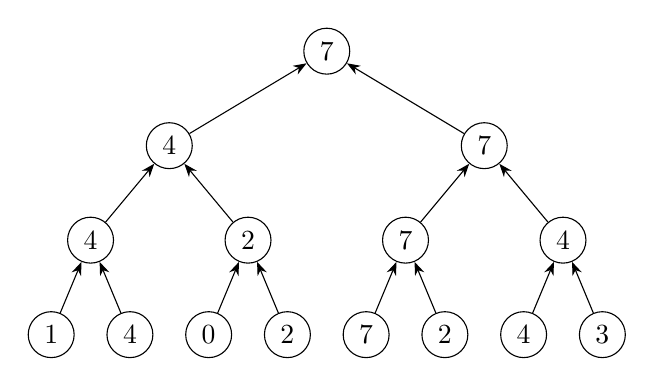
\begin{tikzpicture}
                        [level distance=12mm,
                         level 1/.style={sibling distance=40mm},
                         level 2/.style={sibling distance=20mm},
                         level 3/.style={sibling distance=10mm},
                         every node/.style={draw, circle, inner sep=3pt},
                         edge from parent/.style={draw, {Stealth}-}]

                        \node {7} % Root
                        child {node {4}
                            child {node {4}
                            child {node {1} }
                            child {node {4} }
                            }
                            child {node {2}
                            child {node {0} }
                            child {node {2} }
                            }
                        }
                        child {node {7}
                            child {node {7}
                            child {node {7} }
                            child {node {2} }
                            }
                            child {node {4}
                            child {node {4} }
                            child {node {3} }
                            }
                        };
                    \end{tikzpicture}
                \end{center}
                The comparison made are:
                \begin{enumerate}
                    \item Level 1:
                    \begin{itemize}
                        \item Pairs:
                        \begin{itemize}
                            \item \texttt{max(1, 4)}
                            \item \texttt{max(0, 2)}
                            \item \texttt{max(7, 2)}
                            \item \texttt{max(4, 3)}
                        \end{itemize}
                        \item Result: \texttt{[4, 2, 7, 4]}
                    \end{itemize}

                    \item Level 2:
                    \begin{itemize}
                        \item Pairs:
                        \begin{itemize}
                            \item \texttt{max(4, 2)}
                            \item \texttt{max(7, 4)}
                        \end{itemize}
                        \item Result: \texttt{[4, 7]}
                    \end{itemize}

                    \item Level 3:
                    \begin{itemize}
                        \item Pair: \texttt{max(4, 7)}
                        \item Result: \texttt{[7]}
                    \end{itemize}
                \end{enumerate}
                At this point, the Up-Sweep phase has found the maximum value of the entire array.
            \end{examplebox}

            \item \definitionWithSpecificIndex{Down-Sweep Phase}{Down-Sweep}{}. Use the partial results from the Up-Sweep phase to \textbf{compute the final scan results for all elements in the array}.
            \begin{enumerate}
                \item \textbf{Initialization}: \hl{Begin with an initial value, typically the identity element} (for maximum, it could be negative infinity $-\infty$).
                \item \textbf{Propagate Results}: \hl{Propagate the maximum values back down the tree}, updating the results for each element.
            \end{enumerate}
            \setcounter{example}{36}
            \begin{examplebox}[ (continue): Down-Sweep technique]
                Continuing from the Up-Sweep phase result \texttt{[7]} and the original array \texttt{[1, 4, 0, 2, 7, 2, 4, 3]} (page \hqpageref{example: Up-Sweep (Reduce) technique}).
                
                \highspace
                The main rule followed during the down-sweep technique is the following: the left leaf always inserts the value of the parent node, while the right leaf inserts the value calculated after applying the \texttt{max} operation to the value of the parent node and the left side just removed (which we find on the up-sweep graph).
                
                \highspace
                On the last level of the tree, there is an exception: before inserting the left leaf directly, the \texttt{max} operation of the inherited value and the input value must be performed.

                \highspace
                The steps are detailed:
                \begin{enumerate}
                    \item Replace the maximum value on the root (\texttt{7}) and insert the identity element, in our case the $-\infty$.
                    \begin{center}
                        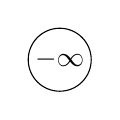
\begin{tikzpicture}
                            [level distance=14mm,
                             level 1/.style={sibling distance=40mm},
                             level 2/.style={sibling distance=20mm},
                             level 3/.style={sibling distance=10mm},
                             every node/.style={draw, circle, minimum size=8mm, inner sep=0pt},
                             edge from parent/.style={draw, -{Stealth}}]
    
                            \node {$-\infty$};
                        \end{tikzpicture}
                    \end{center}
                    \item Level 1:
                    \begin{itemize}
                        \item Insert the parent node on the left leaf, so $-\infty$.
                        \item On the right leaf, insert the performed operation between the parent's value and the left leaf of the up-sweep tree. So the values to compare are $-\infty$ and $4$: \texttt{max($-\infty$, 4) = 4}
                    \end{itemize}
                    \begin{center}
                        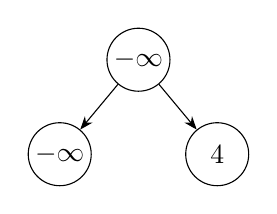
\begin{tikzpicture}
                            [level distance=12mm,
                             level 1/.style={sibling distance=20mm},
                             every node/.style={draw, circle, minimum size=8mm, inner sep=0pt},
                             edge from parent/.style={draw, -{Stealth}}]
    
                            \node {$-\infty$} % Root
                            child {node {$-\infty$}}
                            child {node {4}};
                        \end{tikzpicture}
                    \end{center}
                    \newpage
                    \item Level 2 ((from left to the right)):
                    \begin{itemize}
                        \item Vertex $-\infty$:
                        \begin{itemize}
                            \item Insert the parent node on the \textbf{left leaf}, so $-\infty$. It's not the last leaf of the tree, so we don't do any checking.

                            \item The \textbf{right leaf} comparison is between $-\infty$ (the father's value) and the left leaf on the up-sweep tree (the value just replaced by the $-\infty$), so 4. Again, the comparison is:
                            \begin{equation*}
                                \texttt{max($-\infty$, 4) = 4}
                            \end{equation*}
                        \end{itemize}

                        \item Vertex $4$:
                        \begin{itemize}
                            \item Insert the parent node on the \textbf{left leaf}, so $4$.
                            \item The \textbf{right leaf} comparison is between 4 (the father's value) and the left leaf on the up-sweep tree (the value just replaced by 4), so 7. The comparison is:
                            \begin{equation*}
                                \texttt{max(4, 7) = 7}
                            \end{equation*}
                        \end{itemize}
                    \end{itemize}
                    \begin{center}
                        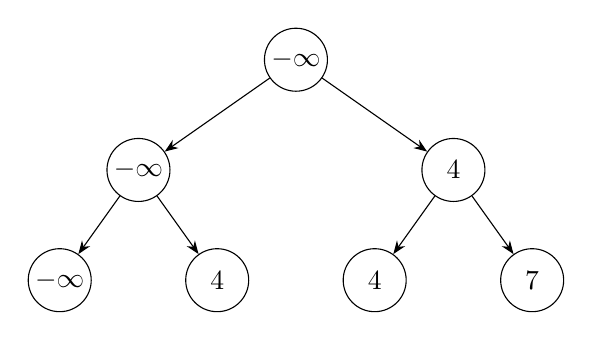
\begin{tikzpicture}
                            [level distance=14mm,
                             level 1/.style={sibling distance=40mm},
                             level 2/.style={sibling distance=20mm},
                             level 3/.style={sibling distance=10mm},
                             every node/.style={draw, circle, minimum size=8mm, inner sep=0pt},
                             edge from parent/.style={draw, -{Stealth}}]
    
                            \node {$-\infty$} % Root
                            child {node {$-\infty$}
                                child {node {$-\infty$}}
                                child {node {4}}
                            }
                            child {node {4}
                                child {node {4}}
                                child {node {7}}
                            };
                        \end{tikzpicture}
                    \end{center}
                    \item Level 3 (from left to the right):
                    \begin{itemize}
                        \item Vertex $-\infty$:
                        \begin{itemize}
                            \item \textbf{Left leaf}. Since this is the last level, we need to compute an extra check. We need to compute:
                            \begin{equation}
                                \texttt{max(inherited val, input val)}
                            \end{equation}\label{eq: down-sweep last level}
                            In our case, the inherited value is the $-\infty$, but the input value on the first position is 1. Therefore:
                            \begin{equation*}
                                \texttt{max($-\infty$, 1) = 1}
                            \end{equation*}
                            \item \textbf{Right leaf}. We compare the value we just removed, 1, to the value of the parent: $-\infty$.
                            \begin{equation*}
                                \texttt{max(1, $-\infty$) = 1}
                            \end{equation*}
                            The result should be 1 \underline{BUT} we are at the last level of the tree. So we need to do an extra check between the inherited value (what we want to place) and the input value on the second position (our case 4):
                            \begin{equation*}
                                \texttt{max(1, 4) = 4}
                            \end{equation*}
                        \end{itemize}
                        \item Vertex $4$:
                        \begin{itemize}
                            \item \textbf{Left leaf}. We apply formula \ref{eq: down-sweep last level} on page \pageref{eq: down-sweep last level}, the idea is the same as before:
                            \begin{equation*}
                                \texttt{max(4, 0) = 4}
                            \end{equation*}
                            \item \textbf{Right leaf}. We compare the value just removed, 0, to the value of parent: 4.
                            \begin{equation*}
                                \texttt{max(0, 4) = 4}
                            \end{equation*}
                            And the value obtained with the input value on the array:
                            \begin{equation*}
                                \texttt{max(4, 2) = 4}
                            \end{equation*}
                        \end{itemize}
                        \item Vertex $4$:
                        \begin{itemize}
                            \item \textbf{Left leaf}. We apply formula \ref{eq: down-sweep last level} on page \pageref{eq: down-sweep last level}, the idea is the same as before:
                            \begin{equation*}
                                \texttt{max(4, 7) = 7}
                            \end{equation*}
                            \item \textbf{Right leaf}. We compare the value just removed, 7, to the value of parent: 4.
                            \begin{equation*}
                                \texttt{max(7, 4) = 7}
                            \end{equation*}
                            And the value obtained with the input value on the array:
                            \begin{equation*}
                                \texttt{max(7, 2) = 7}
                            \end{equation*}
                        \end{itemize}
                        \newpage
                        \item Vertex $7$:
                        \begin{itemize}
                            \item \textbf{Left leaf}. We apply formula \ref{eq: down-sweep last level} on page \pageref{eq: down-sweep last level}, the idea is the same as before:
                            \begin{equation*}
                                \texttt{max(7, 4) = 7}
                            \end{equation*}
                            \item \textbf{Right leaf}. We compare the value just removed, 4, to the value of parent: 7.
                            \begin{equation*}
                                \texttt{max(4, 7) = 7}
                            \end{equation*}
                            And the value obtained with the input value on the array:
                            \begin{equation*}
                                \texttt{max(7, 3) = 7}
                            \end{equation*}
                        \end{itemize}
                    \end{itemize}
                    \begin{center}
                        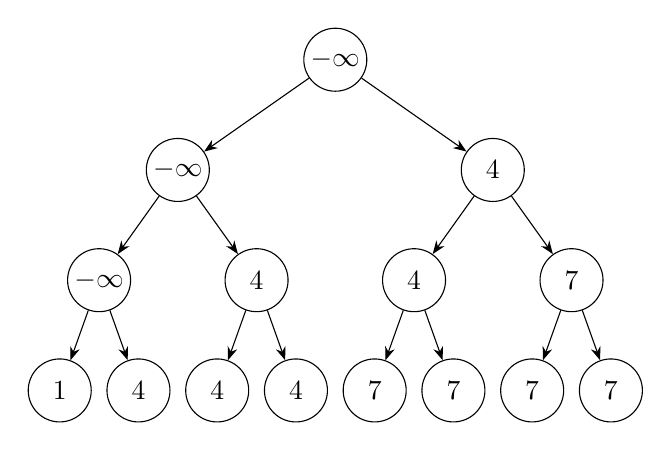
\begin{tikzpicture}
                            [level distance=14mm,
                             level 1/.style={sibling distance=40mm},
                             level 2/.style={sibling distance=20mm},
                             level 3/.style={sibling distance=10mm},
                             every node/.style={draw, circle, minimum size=8mm, inner sep=0pt},
                             edge from parent/.style={draw, -{Stealth}}]
    
                            \node {$-\infty$} % Root
                            child {node {$-\infty$}
                                child {node {$-\infty$}
                                child {node {1} }
                                child {node {4} }
                                }
                                child {node {4}
                                child {node {4} }
                                child {node {4} }
                                }
                            }
                            child {node {4}
                                child {node {4}
                                child {node {7} }
                                child {node {7} }
                                }
                                child {node {7}
                                child {node {7} }
                                child {node {7} }
                                }
                            };
                        \end{tikzpicture}
                    \end{center}
                \end{enumerate}
            \end{examplebox}
        \end{enumerate}
    \end{itemize}
    \begin{figure}[!htp]
        \centering
        \includegraphics[width=.85\textwidth]{img/maximum-up-down-sweep-1.pdf}
        \caption{Graphical example of the Maximum Algorithm with Up and Down Sweep. On the left a sequential version and on the right a parallel version. The parallel version was analyzed on the previous pages.}
    \end{figure}


    \item \definition{Three-Phase Scan with Tiling}
    \begin{itemize}
        \item[\textcolor{Red2}{\faIcon{book}}] \textcolor{Red2}{\textbf{Definition}}. Three-Phase Scan with Tiling is a technique that \textbf{divides the input array into smaller tiles and processes them in three distinct phases} to efficiently perform the scan operation.
        
        The main goal is to improve parallelism and cache efficiency by splitting the input array into smaller tiles and processing them independently.

        \item[\textcolor{Green3}{\faIcon{tools}}] \textcolor{Green3}{\textbf{Algorithm}}
        \begin{enumerate}
            \item \definition{Tiling and Local Scan}. Divide the input array into smaller tiles and perform the scan operation on each tile independently.
            \begin{enumerate}
                \item \textbf{Divide the Input Array}: Break the input array into smaller blocks or tiles.
                \item \textbf{Local Scan} (Inclusive): Compute the scan for each tile independently.
            \end{enumerate}
            \begin{examplebox}[: Tiling and Local Scan]
                For an array \texttt{[1, 2, 3, 4, 5, 6, 7, 8]} with a tile size of 4:
                \begin{itemize}
                    \item Tiles: \texttt{[1, 2, 3, 4]} and \texttt{[5, 6, 7, 8]}
                    \item Local Scans:
                    \begin{itemize}
                        \item First tile: \texttt{[1, 3, 6, 10]}
                        \item Second tile: \texttt{[5, 11, 18, 26]}
                    \end{itemize}
                \end{itemize}
            \end{examplebox}

            \item \definition{Scan of Tile Results}. Compute the \textbf{scan of the final elements of each tile to handle dependencies between tiles}.
            \begin{enumerate}
                \item \textbf{Extract Final Elements}: Take the last element of each tile.
                \item \textbf{Global Scan}: Perform a scan operation on these final elements to propagate the results across tiles.
            \end{enumerate}
            \begin{examplebox}[: Scan of Tile Results]
                \begin{itemize}
                    \item Final Elements: \texttt{10} (from the first tile) and \texttt{26} (from the second tile)
                    \item Global Scan: \texttt{[10, 36]} (assuming addition and identity element \texttt{0})
                \end{itemize}
            \end{examplebox}

            \item \definition{Distribution of Tile Results}. \textbf{Distribute the results of the scanned tile results to all elements in their respective tiles}.
            \begin{enumerate}
                \item \textbf{Distribute Results}: Add the scan results of the previous tiles to the elements of the current tile.
            \end{enumerate}
            \begin{examplebox}[: Distribution of Tile Results]
                \begin{itemize}
                    \item First Tile Remains the Same: \texttt{[1, 3, 6, 10]}
                    \item Second Tile: add the scan result \texttt{10} from the first tile's last element:
                    \begin{itemize}
                        \item \texttt{5 + 10 = 15}
                        \item \texttt{11 + 10 = 21}
                        \item \texttt{18 + 10 = 28}
                        \item \texttt{26 + 10 = 36}
                    \end{itemize}
                    \begin{equation*}
                        \texttt{[15, 21, 28, 36]}
                    \end{equation*}
                \end{itemize}
                Combining the results of the two tiles, we get:
                \begin{equation*}
                    \texttt{[1, 3, 6, 10, 15, 21, 28, 36]}
                \end{equation*}
            \end{examplebox}
        \end{enumerate}
    \end{itemize}
    \begin{figure}[!htp]
        \centering
        \includegraphics[width=\textwidth]{img/three-phase-scan-with-tiling-1.pdf}
        \caption{Graphical example of the Three-Phase Scan with Tiling.}
    \end{figure}


    \item \definition{Fusion of Map Pattern with Scan Pattern}
    \begin{itemize}
        \item[\textcolor{Red2}{\faIcon{book}}] \textcolor{Red2}{\textbf{Definition}}. Combine the transformation capabilities of the map pattern with the cumulative operations of the scan pattern to \textbf{achieve more complex and efficient parallel computations}.
        
        When we fuse the map and scan patterns, we \textbf{first apply the map function to transform each element in the input sequence}, and \textbf{then apply the scan operation to the transformed sequence}.

        \item[\textcolor{Green3}{\faIcon{tools}}] \textcolor{Green3}{\textbf{Algorithm}}
        \begin{enumerate}
            \item \textbf{Apply Map Function}: Transform each element in the input sequence using the map function.
            \item \textbf{Apply Scan Operation}: Perform the scan operation on the transformed sequence to compute cumulative results.
        \end{enumerate}
    \end{itemize}
    \begin{examplebox}[: Fusion of Map Pattern with Scan Pattern]
        Let's consider a practical example where we want to compute the prefix sums of the squares of an input array \texttt{[1, 2, 3, 4]}.
        \begin{enumerate}
            \item \textbf{Map Function}
            \begin{enumerate}
                \item Define the map function as $f\left(x\right) = x^{2}$.
                \item Apply the map function: \texttt{[1, 4, 9, 16]} (squares of the input elements),
            \end{enumerate}
            \item \textbf{Scan Operation}
            \begin{enumerate}
                \item Perform an inclusive scan on the transformed sequence \texttt{[1, 4, 9, 16]}.
                \item Inclusive scan result: \texttt{[1, 5, 14, 30]}.
            \end{enumerate}
        \end{enumerate}
    \end{examplebox}
    \begin{figure}[!htp]
        \centering
        \includegraphics[width=\textwidth]{img/fusion-map-with-scan-1.pdf}
        \caption{Graphical example of the Fusion of Map Pattern with Scan Pattern.}
    \end{figure}
\end{itemize}

    \subsection{Gather Pattern}

\subsubsection{What is a Gather?}

\begin{flushleft}
    \textcolor{Green3}{\faIcon{question-circle} \textbf{Why is the need for the gather pattern born?}}
\end{flushleft}
There are two main reasons for this:
\begin{enumerate}
    \item \important{Data Movement}.

    \textcolor{Red2}{\faIcon{question} \textbf{Problem}}. Data movement is often more costly than computation, especially when transferring data across memory layers or networks. This includes factors like:
    \begin{itemize}
        \item Locality optimization. \hl{Reducing data access times} by keeping frequently accessed data close to the processing unit.
        \item Efficient data access. Improving performance by \hl{minimizing the cost of accessing scattered data locations}.
    \end{itemize}

    \textcolor{Green3}{\faIcon{check} \textbf{Solution}}. The gather pattern addresses these issues by efficiently \hl{collecting data from multiple, scattered memory locations into a contiguous structure}.


    \item \important{Parallel Data Reorganization}.
    
    \textcolor{Red2}{\faIcon{question} \textbf{Problem}}. To achieve performance gains in parallel algorithms, data often needs to be reorganized efficiently. This involves:
    \begin{itemize}
        \item Parallel data movement. \hl{Moving large datasets simultaneously} rather than sequentially.
        \item Consistency management. \hl{Ensuring data integrity} while reorganizing in parallel.
        \item Intermediate data structures. \hl{Holding temporary results during reorganization}.
    \end{itemize}

    \textcolor{Green3}{\faIcon{check} \textbf{Solution}}. The gather pattern is crucial for parallel data reorganization because it:
    \begin{itemize}[label=\textcolor{Green3}{\faIcon{check}}]
        \item \hl{Enables parallel data movement}, allowing multiple data points to be gathered simultaneously from different sources.
        \item \hl{Maintains data consistency}, ensuring that the reorganization process doesn't introduce errors.
        \item \hl{Supports intermediate structures}, making it easier to manage data during complex transformations.
    \end{itemize}
\end{enumerate}

\newpage

\begin{flushleft}
    \textcolor{Green3}{\faIcon{book} \textbf{What is a Gather Pattern?}}
\end{flushleft}
The \definition{Gather Pattern} is a data movement operation that \textbf{creates a new (\emph{source}) collection of data by reading elements from an existing (\emph{input}) data collection}. It is commonly used in parallel computing to efficiently \hl{reorganize} or \hl{extract data based on specific indices}. At first it might seem complicated, but with some simple examples it will be very easy.

\highspace
In general, it works like this:
\begin{enumerate}
    \item \textbf{Read} data from the input collection at positions specified.
    \item \textbf{Write} the gathered data to the output collection in the same order as the indexes specified in Input.
    \item Returns an output collection that has the same shape (or dimensionality) as the index collection.
\end{enumerate}
It can be seen as a \textbf{combination} of \texttt{map} and \texttt{random read} operations because it \textbf{performs multiple reads from non-contiguous memory locations}.

\highspace
\begin{flushleft}
    \textcolor{Green3}{\faIcon{tools} \textbf{\underline{Serial} Implementation}}
\end{flushleft}
The following pseudocode shows a serial implementation of the gather pattern:
\begin{lstlisting}[language=c++]
template<typename Data, typename Idx>
void gather(
    size_t n,    // number of elements in data collection
    size_t m,    // number of elements in index collection
    Data a[],    // input data collection (n elements)
    Data A[],    // output data collection (m elements)
                 // used to modify the output in place
    Idx idx[]    // input index collection (m elements)
) {
    // Iterate over index collection
    for (size_t i = 0; i < m; ++i) {
        // Get the i-th index
        size_t j = idx[i];
        // Ensure index is within bounds;
        // It avoids buffer overflow,
        // and ensure memory safety
        assert(0 <= j && j < n);
        // Perform random read and write to output
        A[i] = a[j];
    }
}
\end{lstlisting}
The pseudo-signature of the function is:
\begin{itemize}
    \item Input:
    \begin{itemize}
        \item \texttt{a[]}: original data collection (size \texttt{n}).
        \item \texttt{idx[]}: index collection specifying which elements to gather (size \texttt{m}).
    \end{itemize}

    \item Output:
    \begin{itemize}
        \item \texttt{A[]}: output collection to store gathered elements (size \texttt{m}, trivial since we iterate over the input indices \texttt{idx})
    \end{itemize}
\end{itemize}
The process performs the following operations:
\begin{enumerate}
    \item \textbf{Loop through each index} \texttt{i} in the index collection (\texttt{idx[]}).
    \item \textbf{Access the data} at position \texttt{idx[i]} in \texttt{a[]}.
    \item \textbf{Assertion} ensures that the index is valid (within the bounds of \texttt{a[]}).
    \item \textbf{Copy the data} from \texttt{a[idx[i]]} to the corresponding position \texttt{A[i]} in the output collection.
\end{enumerate}
It is interesting to note that there are good \textbf{opportunities to parallelize} the code thanks to the for loop. In fact, \hl{each iteration is independent} of the others (no data dependencies between iterations). More precisely, \hl{each thread writes to a unique position in the output} array (collection) \texttt{A}. Also, \hl{each position is valid} thanks to the assert boundary check.

\highspace
\begin{examplebox}[: Gather Pattern]
    Let the following arguments:
    \begin{itemize}
        \item Source Array, contains the original data elements:
        \begin{equation*}
            \texttt{A = [A, B, C, D, E, F, G, H]}
        \end{equation*}
        Indices \texttt{0} through \texttt{7}, so the \texttt{n} argument is \texttt{8}.

        \item Index Array, specifies which elements from the source array to retrieve:
        \begin{equation*}
            \texttt{idx = [1, 5, 0, 2, 2, 4]}
        \end{equation*}
        Indices \texttt{0} through \texttt{5}, so the \texttt{m} argument is \texttt{6}.

        \item Output Array, will store the gathered elements in the order of the indices \texttt{idx}:
        \begin{equation*}
            \texttt{B = []}
        \end{equation*}
        Empty initially, will be filled based on \texttt{idx}.
    \end{itemize}
    The function calculates:
    \begin{enumerate}
        \item First iteration:
        \begin{enumerate}
            \item Get \emph{0}-th index: \texttt{idx[0] = 1}
            \item Boundary check? \texttt{0 <= idx[0] $\land$ idx[0] < 8} \textcolor{Green3}{\faIcon{check}}
            \item Perform random read: \texttt{B[0] = A[idx[0]] = A[1] = B}
        \end{enumerate}
        \item Second iteration:
        \begin{enumerate}
            \item Get \emph{1}-th index: \texttt{idx[1] = 5}
            \item Boundary check? \texttt{0 <= idx[1] $\land$ idx[1] < 8} \textcolor{Green3}{\faIcon{check}}
            \item Perform random read: \texttt{B[1] = A[idx[1]] = A[5] = F}
        \end{enumerate}
        \newpage
        \item Third iteration:
        \begin{enumerate}
            \item Get \emph{2}-th index: \texttt{idx[2] = 0}
            \item Boundary check? \texttt{0 <= idx[2] $\land$ idx[2] < 8} \textcolor{Green3}{\faIcon{check}}
            \item Perform random read: \texttt{B[2] = A[idx[2]] = A[0] = A}
        \end{enumerate}
        \item Fourth iteration:
        \begin{enumerate}
            \item Get \emph{3}-th index: \texttt{idx[3] = 2}
            \item Boundary check? \texttt{0 <= idx[3] $\land$ idx[3] < 8} \textcolor{Green3}{\faIcon{check}}
            \item Perform random read: \texttt{B[3] = A[idx[3]] = A[2] = C}
        \end{enumerate}
        \item Fifth iteration:
        \begin{enumerate}
            \item Get \emph{4}-th index: \texttt{idx[4] = 2}
            \item Boundary check? \texttt{0 <= idx[4] $\land$ idx[4] < 8} \textcolor{Green3}{\faIcon{check}}
            \item Perform random read: \texttt{B[4] = A[idx[4]] = A[2] = C}
        \end{enumerate}
        \item Sixth iteration:
        \begin{enumerate}
            \item Get \emph{5}-th index: \texttt{idx[5] = 4}
            \item Boundary check? \texttt{0 <= idx[5] $\land$ idx[5] < 8} \textcolor{Green3}{\faIcon{check}}
            \item Perform random read: \texttt{B[5] = A[idx[5]] = A[4] = E}
        \end{enumerate}
    \end{enumerate}
    The returned output collection is:
    \begin{equation*}
        \texttt{B = [B, F, A, C, C, E]}
    \end{equation*}
\end{examplebox}

\noindent
Some interesting observations we can make are:
\begin{itemize}
    \item \textbf{Same dimensionality}: output data collection (array \texttt{B}) has the same number of elements as the number of indexes in the index collection (value \texttt{m}).
    \item \textbf{Same types}: elements of the output collection are of the same type as the input data collection.
\end{itemize}
    \subsubsection{Shift}

The \definition{Shift operation} is a specialized case of the gather pattern where \textbf{data is moved uniformly left or right in memory}. Unlike random gathers (already seen in section \ref{subsubsection: What is a Gather}, page \pageref{subsubsection: What is a Gather}), shifts involve \textbf{regular}, \textbf{predictable data movement} with \underline{fixed offsets}.

\highspace
\begin{flushleft}
    \textcolor{Green3}{\faIcon{star} \textbf{Key Features}}
\end{flushleft}
\begin{itemize}
    \item \important{Data Movement}. Elements are \hl{shifted by a fixed distance}.
    \item \important{Offset Access}. Data accesses are offset uniformly, making the operation predictable. 
\end{itemize}

\highspace
\begin{flushleft}
    \textcolor{Red2}{\faIcon{exclamation-triangle} \textbf{Boundary Conditions}}
\end{flushleft}
With the shift operation, the main problem we can encounter is mainly one: boundary conditions.

\highspace
When shifting data, \textbf{handling the edge elements} (out-of-bounds data) \textbf{is crucial}. There are several strategies:
\begin{itemize}[label=\textcolor{Green3}{\faIcon{check}}]
    \item \textcolor{Green3}{\textbf{Default Value}}. Fill the vacant position with a default (e.g., \texttt{0} or \texttt{null}).
    \begin{examplebox}[: Default Boundary Condition]
        Input array:
        \begin{equation*}
            \texttt{A = [1, 2, 3, 4, 5, 6, 7, 8, 9, 10]}
        \end{equation*}
        Shift with default boundary condition:
        \begin{itemize}
            \item Left shift:
            \begin{equation*}
                \texttt{A = [2, 3, 4, 5, 6, 7, 8, 9, 10, 0]}
            \end{equation*}
            \item Right shift:
            \begin{equation*}
                \texttt{A = [0, 1, 2, 3, 4, 5, 6, 7, 8, 9]}
            \end{equation*}
        \end{itemize}
    \end{examplebox}

    \item \textcolor{Green3}{\textbf{Duplicate}}. Replicate the edge element to fill the gap.
    \begin{examplebox}[: Duplicate Boundary Condition]
        Input array:
        \begin{equation*}
            \texttt{A = [1, 2, 3, 4, 5, 6, 7, 8, 9, 10]}
        \end{equation*}
        Shift with duplicate boundary condition:
        \begin{itemize}
            \item Left shift:
            \begin{equation*}
                \texttt{A = [2, 3, 4, 5, 6, 7, 8, 9, 10, 10]}
            \end{equation*}
            \item Right shift:
            \begin{equation*}
                \texttt{A = [1, 1, 2, 3, 4, 5, 6, 7, 8, 9]}
            \end{equation*}
        \end{itemize}
    \end{examplebox}

    \item \textcolor{Green3}{\textbf{Rotate}}. Wrap around the array, moving the last element to the first position (circular shift).
    \begin{examplebox}[: Rotate Boundary Condition]
        Input array:
        \begin{equation*}
            \texttt{A = [1, 2, 3, 4, 5, 6, 7, 8, 9, 10]}
        \end{equation*}
        Shift with rotate boundary condition:
        \begin{itemize}
            \item Left shift:
            \begin{equation*}
                \texttt{A = [2, 3, 4, 5, 6, 7, 8, 9, 10, 1]}
            \end{equation*}
            \item Right shift:
            \begin{equation*}
                \texttt{A = [10, 1, 2, 3, 4, 5, 6, 7, 8, 9]}
            \end{equation*}
        \end{itemize}
    \end{examplebox}
\end{itemize}

\highspace
\begin{flushleft}
    \textcolor{Green3}{\faIcon{tachometer-alt} \textbf{Advantages \& Benefits}}
\end{flushleft}
\begin{itemize}
    \item Shifts are highly efficient with \textbf{vector instructions} due to their regularity.
    \item They allow \textbf{parallel shifting} of multiple elements simultaneously.
    \item Good \textbf{data locality} enhances performance, as adjacent elements are accessed together.
\end{itemize}
    \subsubsection{Zip}

The \definition{Zip operation} is a special case of the gather pattern where \textbf{two (or more) arrays are combined by interleaving their elements}. It functions like a zipper, \textbf{taking one element from each array in sequence to form a new combined array}. It is important to note that it \textbf{works with different types}, so we can zip elements of different types, like integers and floats, or even complex objects.

\highspace
\begin{flushleft}
    \textcolor{Green3}{\faIcon{tools} \textbf{How does it work?}}
\end{flushleft}
The operation \textbf{takes an element from the first array}, then \textbf{one from the second} array, another from the third, and so on, and \textbf{repeats the process}. The \textbf{output is the combined sequence}.
\begin{examplebox}[: zip operation]
    Consider two arrays:
    \begin{enumerate}
        \item Real Parts: contains real numbers.
        \item Imaginary Parts: contains imaginary numbers.
    \end{enumerate}
    The output is a combined sequence like:
    \begin{equation*}
        \texttt{[Real0, Imag0, Real1, Imag1, Real2, Imag2, ...]}
    \end{equation*}
    \begin{center}
        \includegraphics[width=.7\textwidth]{img/zip-1.pdf}
    \end{center}
\end{examplebox}

\highspace
\begin{flushleft}
    \textcolor{Green3}{\faIcon{tachometer-alt} \textbf{Parallelism}}
\end{flushleft}
Each pair of elements (one from each array) can be \textbf{combined independently}. This independence allows \textbf{parallel execution since there's no dependency between the operations for different pairs}.

    \subsubsection{Unzip}

The \definition{Unzip operation} is essentially the \textbf{reverse of the zip operation}. While zip combines multiple arrays into one by interleaving their elements, \textbf{unzip separates a single interleaved array back into its original components}.

\highspace
\begin{flushleft}
    \textcolor{Green3}{\faIcon{tools} \textbf{How does it work?}}
\end{flushleft}
The operation \textbf{extracts sub-arrays at regular offsets} (strides) \textbf{to separate the elements into their original groups}. The input is a combined sequence (e.g., alternating real and imaginary parts).
\begin{examplebox}[: unzip operation]
    Consider the input array:
    \begin{equation*}
        \texttt{[Real0, Imag0, Real1, Imag1, Real2, Imag2, ...]}
    \end{equation*}
    The output are:
    \begin{itemize}
        \item Array of Real Parts: \texttt{[Real0, Real1, Real2]}
        \item Array of Imaginary Parts: \texttt{[Imag0, Imag1, Imag2]}
    \end{itemize}
    \begin{center}
        \includegraphics[width=.7\textwidth]{img/unzip-1.pdf}
    \end{center}
\end{examplebox}

\highspace
\begin{flushleft}
    \textcolor{Green3}{\faIcon{tachometer-alt} \textbf{Parallelism}}
\end{flushleft}
Each element extraction is independent. This allows for \textbf{parallel data access} because there's no dependency between different extractions.

\highspace
However, the unzip operation is an \textbf{efficient data extraction because it takes advantage of stride-based memory access}, which can be optimized for performance.
    \subsection{Scatter Pattern}

\subsubsection{What is a Scatter?}

The \definition{Scatter Pattern} is a data movement pattern where \textbf{elements from a source array are distributed (or scattered) to various locations in a destination array based on specified indices}. Essentially, it's about writing data to random locations.

\highspace
\begin{flushleft}
    \textcolor{Green3}{\faIcon{star} \textbf{Key Features}}
\end{flushleft}
In general, the \textbf{input} of the scatter pattern is:
\begin{itemize}
    \item \textbf{Source data array}: value to be written.
    \item \textbf{Index array}: specifies where each value should be written in the destination.
\end{itemize}
Each element from the source is written to the position in the target array specified by the corresponding index. The \textbf{output is a target array where the data is scattered across the positions}.

\highspace
\begin{flushleft}
    \textcolor{Green3}{\faIcon{balance-scale} \textbf{Gather vs. Scatter}}
\end{flushleft}
The main differences between gather and scatter are:
\begin{itemize}
    \item \important{Gather} (read focused): Involves \textbf{random reads} where the read \textbf{locations are provided as input}.
    \item \important{Scatter} (write focused): Involves \textbf{random writes} with write \textbf{locations provided as input}, which can lead to race conditions.
\end{itemize}

\highspace
\begin{flushleft}
    \textcolor{Green3}{\faIcon{tools} \textbf{\underline{Serial} implementation}}
\end{flushleft}
The following pseudocode shows a serial implementation of the scatter pattern:
\begin{lstlisting}[language=c++]
template<typename Data, typename Idx>
void scatter(
    size_t n,     // Number of elements
                  // in the output data collection
    size_t m,     // Number of elements
                  // in the input data and index collection
    Data a[],     // Input data collection (m elements)
    Data A[],     // Output data collection (n elements)
    Idx idx[]     // Input index collection (m elements)
) {
    // Loop through each input element
    for (size_t i = 0; i < m; ++i) {
        // Get the target index from the index array
        size_t j = idx[i];
        // Ensure the index is within output array bounds
        assert(0 <= j && j < n);
        // Perform the scatter: write a[i] to A[j]
        A[j] = a[i];
    }
}
\end{lstlisting}
The method is characterized by:
\begin{itemize}
    \item \important{Loop} (\texttt{for}): Iterates through each element in the input array \texttt{a[]} (length \texttt{m}).
    \item \important{Indexing} (\texttt{j = idx[i]}): Determines \textbf{where to place} \texttt{a[i]} in the output array \texttt{A[]}.
    \item \important{Boundary Check} (\texttt{assert}): Ensures the index \texttt{j} is \textbf{valid} (avoids out-of-bounds errors).
    \item \important{Write Operation} (\texttt{A[j] = a[i]}): \textbf{Scatters} the data from \texttt{a[i]} to \texttt{A[j]}.
\end{itemize}
The possibilities to parallelize the code are interesting, but instead of the gather pattern, here we have a problem with race conditions on write operations. So the code can be parallelized (\textbf{parallelize over for loop to perform random write}), but we \hl{need to find some strategies to avoid race conditions}.

\highspace
\begin{flushleft}
    \textcolor{Red2}{\faIcon{exclamation-triangle} \textbf{Race Conditions in Scatter}}
\end{flushleft}
Unfortunately, the scatter pattern can lead to race conditions because of the way it handles writes to memory. As we know, a race condition occurs when two or more operations try to access and modify the same data at the same time, and the final result depends on the order in which the operations are performed.

\highspace
In the scatter pattern, we're performing random writes to different locations in memory. The \textbf{problem arises when multiple write operations target the same location at the same time}. Because the \hl{writes happen in parallel}, we can't predict:
\begin{enumerate}
    \item Which write will happen first
    \item Which value will be stored last
\end{enumerate}

\highspace
\begin{examplebox}[: Race Condition in Scatter]
    Consider this:
    \begin{itemize}
        \item Source Data:
        \begin{equation*}
            \texttt{A = [A, B, C, D, E, F]}
        \end{equation*}
        \item Index Array (write locations):
        \begin{equation*}
            \texttt{idx = [1, 5, 0, 2, 2, 4]}
        \end{equation*}
    \end{itemize}
    This means that the two threads that will handle the 3rd and 4th positions on the index array will suffer from a race condition. Because if they try to write at the same time, the result will depend on which thread finishes last:
    \begin{itemize}
        \item If thread A (writing \texttt{D}) finishes last, position \texttt{2} will be equal to \texttt{D}.
        \item If thread B (writing \texttt{E}) finishes last, position \texttt{2} will be equal to \texttt{E}.
    \end{itemize}
\end{examplebox}

\newpage

\begin{flushleft}
    \textcolor{Green3}{\faIcon{\speedIcon} \textbf{Optimizing Performance: Converting Scatter to Gather}}
\end{flushleft}
Scatter operations are generally more expensive than gather operations because of how data is written to memory:
\begin{itemize}[label=\textcolor{Red2}{\faIcon{times}}]
    \item \textcolor{Red2}{\textbf{Cache Line Issues}}. Writing data to memory can cause \textbf{cache conflicts}, making memory access slower.
    \item \textcolor{Red2}{\textbf{False Sharing Problem}}. If \textbf{multiple CPU cores write to different parts of the same cache line}, they interfere with each other, slowing down performance.
\end{itemize}
So we can switch to gather pattern to improve performance. Unfortunately, this speedup can \textbf{only be achieved if we know the memory addresses in advance}.

\highspace
\textcolor{Green3}{\faIcon{question-circle} \textbf{So it is only a low-level knowledge?}} Let's get this straight.
\begin{itemize}
    \item[\textcolor{Green3}{\faIcon{check}}] \textcolor{Green3}{\textbf{When we know the memory addresses in advance}}
    \begin{itemize}
        \item It is a scenario where the scatter operation follows a \hl{fixed, predictable pattern}; or the indices where data will be written are statically determined (at compile time) or precomputed before execution. Also, if the same scattering pattern is reused multiple times, precomputing the addresses is worthwhile.

        \begin{examplebox}[: when we know the memory addresses in advance]
            Suppose we're implementing matrix transposition, and each element moves to a fixed new location. The scatter indices can be precomputed once, and instead of writing directly, we gather the elements and write them sequentially.
        \end{examplebox}
    \end{itemize}

    \item[\textcolor{Red2}{\faIcon{times}}] \textcolor{Red2}{\textbf{When we don't know the memory addresses in advance}}
    \begin{itemize}
        \item It is a scenario where the \hl{target indexes depend on runtime data} (e.g., calculation results or user input); or the distribution pattern is dynamic and unpredictable, changing with each execution. Also, when data distribution is affected by real-time conditions, such as load balancing in parallel computing.
    
        \begin{examplebox}[: when we don't know the memory addresses in advance]
            Suppose we are sorting numbers in parallel using a scatter operation, but the final positions depend on comparisons performed at runtime. Since the scatter addresses are computed on the fly, we can't precompute an equivalent gather operation.
        \end{examplebox}
    \end{itemize}
\end{itemize}
So \hl{if the pattern is known in advance, we can convert scatter to gather to improve performance}. But if the \hl{pattern is dynamic}, we have to deal with unpredictable memory writes, leading to potential performance \hl{problems like cache contention and atomic conflicts}.
    \subsubsection{Avoid race conditions}

\paragraph{Atomic Scatter}

\definition{Atomic Scatter} is a \textbf{collision resolution strategy} used when multiple threads attempt to write to the same memory location simultaneously. It is based on one of the most common and famous topic: \textbf{atomic operations}.

\highspace
\begin{flushleft}
    \textcolor{Green3}{\faIcon{question-circle} \textbf{How does it work?}}
\end{flushleft}
\begin{itemize}
    \item[\textcolor{Green3}{\faIcon{check}}] \textcolor{Green3}{\textbf{Atomic Writes}}. \textbf{Each write is atomic}, meaning it either \hl{completes fully or doesn't happen at all}. No partial writes.

    \item[\textcolor{Red2}{\faIcon{times}}] \textcolor{Red2}{\textbf{Non-Deterministic Outcome}}. Since it relies solely on atomic writes, this doesn't mean that there is a mechanism to check which thread should write before another. \hl{When a collision occurs, the outcome depends on which write completes first}. There's no predefined rule for determining which value to store.
\end{itemize}

\highspace
\begin{examplebox}[: Atomic Scatter]
    Consider this:
    \begin{itemize}
        \item Source Data:
        \begin{equation*}
            \texttt{A = [A, B, C, D, E, F]}
        \end{equation*}
        \item Index Array (write locations):
        \begin{equation*}
            \texttt{idx = [1, 5, 0, 2, 2, 4]}
        \end{equation*}
    \end{itemize}
    Notice that each thread is assigned to every position of the \texttt{idx} array. This means that threads \#4 and \#5 must write to the same position on the output array. However, we adopt the atomic strategies so that what happens depends on the order of writing.

    \highspace
    A possibles scenario:
    \begin{enumerate}
        \item Thread \#4 asks to do an atomic write to position 2 of the output array. The operation is marked atomic and can be done safely. The value written to \texttt{A[2]} is \texttt{D}.
        \item Then thread \#5 performs the same steps and overwrites the value written by thread \#4 and writes the value \texttt{E} to \texttt{A[2]}.
    \end{enumerate}
    This is non-deterministic, so this is a possible scenario, but it could also be the other way around and the final value could be \texttt{D}.
\end{examplebox}

\newpage

\begin{flushleft}
    \textcolor{Green3}{\faIcon{check-circle} \textbf{Advantages}}
\end{flushleft}
\begin{itemize}[label=\textcolor{Green3}{\faIcon{check}}]
    \item \textcolor{Green3}{\textbf{Simple to implement}}. No need for complex locking mechanisms.
    \item \textcolor{Green3}{\textbf{Fast}}. Atomic \hl{operations are optimized in hardware}, making them efficient for parallel execution.
\end{itemize}

\highspace
\begin{flushleft}
    \textcolor{Red2}{\faIcon{times-circle} \textbf{Disadvantages}}
\end{flushleft}
\begin{itemize}[label=\textcolor{Red2}{\faIcon{times}}]
    \item \textcolor{Red2}{\textbf{Unpredictable results}}. Non-determinism can be \hl{problematic for algorithms that require consistent outputs}.
    \item \textcolor{Red2}{\textbf{Data loss}}. \hl{One of the colliding values will be lost} without any mechanism to combine or preserve both.
\end{itemize}

\highspace
\begin{flushleft}
    \textcolor{Green3}{\faIcon{question-circle} \textbf{When to use Atomic Scatter?}}
\end{flushleft}
Atomic scatter is suitable when:
\begin{itemize}
    \item \textbf{Collisions are rare}: so the occasional data loss or non-determinism is acceptable.
    \item \textbf{We don't care which value is kept}: for example, in random sampling or approximate algorithms.
\end{itemize}
    \paragraph{Permutation Scatter}

\definition{Permutation Scatter} is a special type of scatter pattern where \textbf{collisions are strictly prohibited}. This means that \textbf{every input element must be placed in a unique output position}, ensuring that the output is a permutation (reordering) of the input.

\highspace
\begin{flushleft}
    \textcolor{Green3}{\faIcon{star} \textbf{Key Features}}
\end{flushleft}
\begin{itemize}
    \item \important{Collisions are illegal}. Unlike atomic scatter, where collisions are resolved non-deterministically, \textbf{permutation scatter ensures that \underline{no} two elements try to write to the same location}.
    \item \important{Output is a permutation of the input}. The output array consists of the same elements as the input but in a different order, \textbf{without any duplicates or missing values}.
    \item \important{Collision checking in advance}. To \hl{guarantee uniqueness}, a \textbf{pre-check must be done} to detect any duplicate indices \textbf{before executing the scatter operation}.
    
    \highspace
    \begin{flushleft}
        \textcolor{Red2}{\faIcon{question-circle} \textbf{What if there is a collision during the pre-check?}}
    \end{flushleft}
    If collisions exist, scatter cannot proceed as-is and may \textbf{need to be transformed into a gather operation} instead.

    \highspace
    \begin{flushleft}
        \textcolor{Green3}{\faIcon{question-circle} \textbf{Why convert a scatter to a gather?}}
    \end{flushleft}
    Instead of letting multiple elements write to the same index in parallel (scatter), we can:
    \begin{enumerate}
        \item Detect collisions beforehand by checking for duplicate indices in the index array.
        \item Reformulate the operation as a gather, where \textbf{each output index reads from a unique input location}, instead of multiple inputs writing to the same index.
        \item Ensure correctness by enforcing a one-to-one mapping between input and output locations.
    \end{enumerate}
    So it is clear that the \textbf{gather ensures that each output location reads from only one input, eliminating write conflicts}.

    \begin{examplebox}[: Convert Scatter to Gather]
        Image we have an input array and an index array:
        \begin{itemize}
            \item Input: \texttt{A = [A, B, C, D]}
            \item Index: \texttt{idx = [1, 3, 3, 2]}
        \end{itemize}
        Here we have a conflict at index 3 because both B and C want to write here. Therefore, the pre-check reports this conflict; the operation has been marked as undefined behavior; we convert the operation from a scatter to a gather.

        \highspace
        Now the approaches we can make are two: we \textbf{convert the whole operation} into a gather and we do that in parallel (to achieve high performance); or the \textbf{position where the permutation cannot guarantee the atomic write, are passed to a gather function to guarantee atomicity}.

        \highspace
        The implementation depends on the programmer and the behavior we want. What we need to know is that: \textbf{if a conflict is detected during permutation, the conversion to gather is the best choice that we can make}.
    \end{examplebox}

    Permutation scatter requires a one-to-one mapping between input and output indices. If collisions exist, scatter must be \textbf{turned into gather so that instead of multiple inputs writing to the same location, each output position retrieves its correct value without conflicts}.
\end{itemize}

\highspace
\begin{flushleft}
    \textcolor{Green3}{\faIcon{balance-scale} \textbf{Permutation vs. Atomic Scatter}}
\end{flushleft}
\begin{itemize}
    \item \important{Collision}
    \begin{itemize}
        \item \textbf{Atomic}: Allowed, resolved arbitrarily.
        \item \textbf{Permutation}: Not allowed.
    \end{itemize}
    \item \important{Write conflicts}
    \begin{itemize}
        \item \textbf{Atomic}: Handled using atomic operations.
        \item \textbf{Permutation}: Avoided by pre-checking
    \end{itemize}
    \item \important{Output structure}
    \begin{itemize}
        \item \textbf{Atomic}: Can overwrite values.
        \item \textbf{Permutation}: Always a permutation of input.
    \end{itemize}
    \item \important{Use Cases}
    \begin{itemize}
        \item \textbf{Atomic}: Hash tables, parallel memory writes.
        \item \textbf{Permutation}: Matrix transposition, FFT scrambling.
    \end{itemize}
\end{itemize}

    \paragraph{Merge Scatter}

The \definition{Merge Scatter} strategy is a way to resolve write conflicts in a scatter operation by \textbf{applying a merge operator that combines values instead of discarding or randomly selecting one}.  

\highspace
\begin{flushleft}
    \textcolor{Green3}{\faIcon{tools} \textbf{How does it work?}}
\end{flushleft}
Instead of letting one thread overwrite another's data, Merge Scatter \textbf{applies a merge function to combine values when a conflict occurs}. The \hl{function must be}:
\begin{itemize}
    \item \important{Associative}, order of grouping doesn't change result:
    \begin{equation*}
        \left(a \oplus b\right) \oplus c = a \oplus \left(b \oplus c\right)
    \end{equation*}
    \item \important{Commutative}, order of values doesn't change result:
    \begin{equation*}
        a \oplus b = b \oplus a
    \end{equation*}
\end{itemize}
\textcolor{Green3}{\faIcon{question-circle} \textbf{Why these properties?}} Because parallel execution means that scatter operations happen in arbitrary order, so the \textbf{merge result must be independent of the order in which values arrive}. In other words, \hl{it guarantees deterministic behavior} (because we always know what the result will be).

\highspace
\begin{examplebox}[: Merge Scatter]
    Suppose we have the following data:
    \begin{center}
        \begin{tabular}{@{} l | l @{}}
            \toprule
            Input   & \texttt{[2, 3, 1, 1, 5, 6]} \\
            Indices & \texttt{[1, 5, 0, 2, 2, 4]} \\
            \bottomrule
        \end{tabular}
    \end{center}
    Positions \texttt{3} and \texttt{4} have multiple writes, causing collisions. Therefore, we use the merge scatter strategy and we define the merge function as: addition.

    \highspace
    So instead of overwriting, we sum the values in case of a conflict:
    \begin{equation*}
        \texttt{[1, 2, 6, \_, 6, 3]}
    \end{equation*}
    At the second position, the index where there was a collision, the merge function was applied between the value \texttt{1} and \texttt{5} (\texttt{1 + 5 = 6}).
\end{examplebox}

\highspace
\begin{flushleft}
    \textcolor{Green3}{\faIcon{check-circle} \textbf{Advantages}}
\end{flushleft}
\begin{itemize}[label=\textcolor{Green3}{\faIcon{check}}]
    \item \textcolor{Green3}{\textbf{Preserves Data}}. Unlike atomic scatter (where some values are lost), merge scatter ensures \textbf{all data contributes to the final output}.
    \item \textcolor{Green3}{\textbf{Parallel-Friendly}}. Works well in parallel settings since \textbf{order doesn't affect the result}.
    \item \textcolor{Green3}{\textbf{Useful in some scenario}}: histogram computation, sparse matrix operations, parallel reductions.
\end{itemize}

\highspace
\begin{flushleft}
    \textcolor{Red2}{\faIcon{times-circle} \textbf{Disadvantages}}
\end{flushleft}
\begin{itemize}[label=\textcolor{Red2}{\faIcon{times}}]
    \item \textcolor{Red2}{\textbf{Increased Computational Overhead}}. Instead of a simple write operation, we now have to \textbf{perform a merge operation} (e.g., addition, \texttt{max}, \texttt{min}). This \textbf{adds extra computational cost}, especially if the merge function is complex. Also, some architectures may require atomic operations or locks to ensure safe merging, which can slow down execution.

    In summary, the \textbf{more conflicts there are, the more overhead is introduced by the merge function}.

    \item \textcolor{Red2}{\textbf{Not Always Deterministic}}. If the merge \textbf{function is not associative and commutative}, the \textbf{result can depend on the order of execution}, which is unpredictable in parallel settings.
    
    Note that this is very common in real-world scenarios; for \example{example}, when using floating-point addition, different execution orders can result in small numerical inconsistencies due to floating-point precision issues.
    
    \item \textcolor{Red2}{\textbf{Possible Loss of Information}}. If the \textbf{merge function is not a lossless operation}, \textbf{some original data might be lost}.
    
    \begin{examplebox}[: Loss of Information]
        For example, if the merge function is \texttt{max()}, only the largest value survives, and all others are discarded. This mean \textbf{we cannot reconstruct the original inputs from the output}.
    \end{examplebox}
    
    \item \textcolor{Red2}{\textbf{Limited Applicability}}. Merge Scatter is \textbf{only applicable when a meaningful merge function exists}. Some applications require exact values, and merging (e.g., summing or taking max) may not be acceptable.
    
    \begin{examplebox}[: Limited Applicability]
        For example, if each thread writes a different pixel color in an image processing task, merging colors with sum/max may produce unintended artifacts.
    \end{examplebox}
\end{itemize}
So we can summarize \textbf{when we need to avoid merge scatter}:
\begin{itemize}[label=\textcolor{Red2}{\faIcon{times}}]
    \item When we need \textcolor{Red2}{\textbf{exact values}} without modification.
    \item When the merge function is \textcolor{Red2}{\textbf{not associative or commutative}}.
    \item When merging \textcolor{Red2}{\textbf{significantly increases computational complexity}}.
\end{itemize}
    \paragraph{Priority Scatter}

\definition{Priority Scatter} is a collision resolution strategy where \textbf{each element in the input array is assigned a priority value} based on its position (or another criterion). When multiple threads attempt to write to the same memory location, the \textbf{element with the highest priority wins}, and the others are discarded.

\highspace
\begin{flushleft}
    \textcolor{Green3}{\faIcon{star} \textbf{Key Features \& Advantages}}
\end{flushleft}
\begin{itemize}
    \item \textbf{Predefined Priority System}. \hl{Each element has a priority}, which could be based on position, timestamp, depth, or another factor.

    \item[\textcolor{Green3}{\faIcon{check}}] \textcolor{Green3}{\textbf{Deterministic Resolution}}. Unlike Atomic Scatter, where race conditions make the final result unpredictable, Priority Scatter \textbf{ensures a well-defined winner}.
    
    \item[\textcolor{Green3}{\faIcon{check}}] \textcolor{Green3}{\textbf{Common in 3D Graphics}}. In 3D rendering, when multiple objects overlap at the same pixel, the object closest to the camera (highest priority) is displayed.
\end{itemize}

\highspace
\begin{flushleft}
    \textcolor{Red2}{\faIcon{times-circle} \textbf{Disadvantages}}
\end{flushleft}
\begin{itemize}[label=\textcolor{Red2}{\faIcon{times}}]
    \item \important{Loss of Information}. Lower-priority elements are discarded entirely.
    \item \important{Predefined Priority Needed}. Requires an external ranking mechanism.
    \item \important{Not Always Fair}. Some data might consistently dominate, suppressing important contributions.
\end{itemize}

\highspace
\begin{flushleft}
    \textcolor{Green3}{\faIcon{balance-scale} \textbf{Comparison Atomic vs. Merge vs. Priority Scatter}}
\end{flushleft}
\begin{table}[!htp]
    \centering
    \begin{tabular}{@{} l l l @{}}
        \toprule
        Strategy & \textbf{Resolution Mechanism} & \textbf{Result Type} \\
        \midrule
        \textbf{Atomic}     & First write wins (random)     & Non-deterministic \\
        \textbf{Merge}      & Merges values (e.g. \texttt{sum}/\texttt{max})  & Aggregated \\
        \textbf{Priority}   & Highest-priority wins         & Deterministic \\
        \bottomrule
    \end{tabular}
    \caption{Differences between Scatter strategies.}
\end{table}

    \subsection{Pack Pattern}

\subsubsection{What is a Pack?}

The \definition{Pack Pattern} is used to \textbf{remove unused elements from a collection while keeping the retained elements contiguous in memory}. The goal is to \textbf{improve performance by reducing memory fragmentation and increasing data locality}, which benefits cache efficiency.

\highspace
\begin{flushleft}
    \textcolor{Green3}{\faIcon{tools} \textbf{How the Pack Algorithm works}}
\end{flushleft}
\begin{enumerate}
    \item \textbf{Convert the input array into Boolean values}. Each element is mapped to \texttt{1} (\emph{keep}) or \texttt{0} (\emph{discard}).
    \item \textbf{Perform an exclusive scan (prefix sum) on the Boolean array}. This step computes the new positions (offsets) of the retained elements.
    \item \textbf{Use the computed offsets to move retained elements to their new locations}. The elements corresponding to \texttt{1}'s in the Boolean array are copied to their new positions.
\end{enumerate}
\begin{examplebox}[: Pack Pattern]
    We have an input array and a mask that tells us which elements to keep (\texttt{1}) and which to remove (\texttt{0}):
    \begin{equation*}
        \begin{array}{rcl}
            \texttt{Index}          & = & \texttt{[0, 1, 2, 3, 4, 5, 6, 7]} \\ [.5em]
            \texttt{Input}          & = & \texttt{[A, B, C, D, E, F, G, H]} \\ [.5em]
            \texttt{Keep (Mask)}    & = & \texttt{[0, 1, 1, 0, 0, 1, 1, 1]}
        \end{array}
    \end{equation*}
    We want to create a new array with only the elements marked \texttt{1}, but we don't yet know \emph{where} to place them.

    The exclusive scan (prefix sum) on the \texttt{Keep} array calculates the new indices for the elements we want to keep.

    We compute the scan using addition (starting from \texttt{0}):
    \begin{equation*}
        \begin{array}{rcl}
            \texttt{Index}                      & = & \texttt{[0, 1, 2, 3, 4, 5, 6, 7]} \\ [.5em]
            \texttt{Keep (Mask)}                & = & \texttt{[0, 1, 1, 0, 0, 1, 1, 1]} \\ [.5em]
            \texttt{Exclusive Scan (New Index)} & = & \texttt{[0, 0, 1, 2, 2, 2, 3, 4]}
        \end{array}
    \end{equation*}
    The scan tells us:
    \begin{itemize}
        \item \texttt{B} goes to index 0
        \item \texttt{C} goes to index 1
        \item \texttt{F} goes to index 2
        \item \texttt{G} goes to index 3
        \item \texttt{H} goes to index 4
    \end{itemize}
    \begin{equation*}
        \texttt{[B, C, F, G, H]}
    \end{equation*}
\end{examplebox}

\highspace
\begin{flushleft}
    \textcolor{Green3}{\faIcon{question-circle} \textbf{Why is Packing Useful?}}
\end{flushleft}
\begin{itemize}
    \item \textcolor{Green3}{\textbf{Reduces memory waste}} by eliminating unnecessary elements.
    \item \textcolor{Green3}{\textbf{Improves data locality}} (sequential memory access is faster than scattered access).
    \item \textcolor{Green3}{\textbf{Boosts cache efficiency}}, reducing cache misses and improving parallel performance.
\end{itemize}

\highspace
\begin{flushleft}
    \textcolor{Red2}{\faIcon{book} \textcolor{Red2}{\textbf{What is the inverse of the Pack pattern?}}}
\end{flushleft}
The \definition{Unpack Pattern} is the inverse of packing. It \textbf{restores the packed elements to their original positions} in an expanded array, reintroducing gaps where necessary.

\highspace
\begin{flushleft}
    \textcolor{Green3}{\faIcon{tools} \textbf{How Unpacking Works}}
\end{flushleft}
Given the same Boolean mask used in packing, unpacking spreads elements back to their original locations, \textbf{leaving empty slots where elements were previously removed}.
\begin{enumerate}
    \item Start with the packed array and the original mask.
    \item Read the mask to decide where elements should go:
    \begin{itemize}
        \item If 1, we take the next packed element.
        \item If 0, we insert a placeholder (empty slot).
    \end{itemize}
    \item Reconstruct the original array.
\end{enumerate}

\begin{examplebox}[: Unpack Pattern]
    We have:
    \begin{enumerate}
        \item The packed array: \texttt{[B, C, F, G, H]}
        \item The original mask: \texttt{[0, 1, 1, 0, 0, 1, 1, 1]}
    \end{enumerate}
    Now we will restore elements using the mask:
    \begin{itemize}
        \item If \texttt{Keep (Mask) = 1}, we copy the next element from the packed array into that position.
        \item If \texttt{Keep (Mask) = 0}, we insert an empty slot (or default value).
    \end{itemize}
    Finally, we place elements back into their original positions using the mask:
    \begin{equation*}
        \begin{array}{rcl}
            \texttt{Index}          & = & \texttt{[0, 1, 2, 3, 4, 5, 6, 7]} \\ [.5em]
            \texttt{Restored Value} & = & \texttt{[\_, B, C, \_, \_, F, G, H]}
        \end{array}
    \end{equation*}
\end{examplebox}

\newpage

\begin{flushleft}
    \textcolor{Green3}{\faIcon{\speedIcon} \textbf{Fusion of Map and Pack: Efficient Filtering of Results}}
\end{flushleft}
The \textbf{fusion of map and pack patterns} is an optimization technique that \textbf{improves efficiency when many elements in a map operation are discarded} (see map pattern on page \pageref{subsection: Map Pattern})

\highspace
The key idea is that \hl{Map pattern applies a function to each element} (e.g., checking for collisions) and \hl{Pack pattern removes unnecessary elements}, storing only meaningful results.

\highspace
This fusion ensures that \textbf{only relevant results are stored and transmitted}, reducing unnecessary computations and memory usage.
\begin{enumerate}
    \item \important{Map checks for collisions}. \textbf{Each element is processed using a mapping function}, which determines whether the element should be kept or discarded. Some elements fail the check.
    \item \important{Pack stores only actual collisions}. \textbf{Only elements that passed the check} (e.g., \texttt{B, C, F, G, H}) \textbf{are stored in the output}. Elements that failed the check (e.g., \texttt{A, D, E}) are removed. The output contains only relevant elements, avoiding unnecessary storage.
    \item \important{Reduces output bandwidth}. The output size depends on valid results, not on the total number of inputs. This is \textbf{beneficial when most of the input elements are discarded}.
    \item \important{Selective output}. Unlike map-only operations, where each input produces an output, \textbf{this fusion allows selective output}.
\end{enumerate}

    \subsubsection{Split}

The \definition{Split operation} is an \hl{extension of the Pack pattern}, but instead of removing elements, it \textbf{reorganizes them into \underline{exactly} two groups while preserving all data} (If there are more than two groups, it is a bin operation, see page \pageref{subsubsection: Bin}).

\highspace
\begin{flushleft}
    \textcolor{Green3}{\faIcon{tools} \textbf{How does Split work?}}
\end{flushleft}
\begin{enumerate}
    \item Each element has a corresponding state (0 or 1).
    \item Instead of discarding elements, as in the normal Pack operation, elements are \textbf{moved into two separate regions} in the output array.
    \item Elements with one state (e.g., 0) go to the first half, while elements with the other state (e.g., 1) go to the second half.
\end{enumerate}

\highspace
\begin{examplebox}[: Split operation]
    We have:
    \begin{equation*}
        \begin{array}{rcl}
            \texttt{Input elements} &=& \texttt{[A, B, C, D, E, F, G, H]} \\ [.5em]
            \texttt{Binary Condition (Mask)} &=& \texttt{[1, 0, 0, 1, 1, 0, 0, 0]}
        \end{array}
    \end{equation*}
    What we do is:
    \begin{enumerate}
        \item Classify elements:
        \begin{itemize}
            \item Elements corresponding to 0: \texttt{[B, C, F, G, H]}
            \item Elements corresponding to 1: \texttt{[A, D, E]}
        \end{itemize}
        \item Place Elements in two groups:
        \begin{itemize}
            \item Upper half (0s first): \texttt{[B, C, F, G, H]}
            \item Lower half (1s second): \texttt{[A, D, E]}
        \end{itemize}
    \end{enumerate}
    And the result is:
    \begin{equation*}
        \texttt{[B, C, F, G, H, A, D, E]}
    \end{equation*}
\end{examplebox}

\highspace
\begin{flushleft}
    \textcolor{Green3}{\faIcon{balance-scale} \textbf{Differences between Pack and Split}}
\end{flushleft}
\begin{table}[!htp]
    \centering
    \begin{tabular}{@{} l | c c @{}}
        \toprule
        \textbf{Feature} & \textbf{Pack} & \textbf{Split} \\
        \midrule
        Removes elements? & \textcolor{Green3}{\faIcon{check}} & \textcolor{Red2}{\faIcon{times}} \\
        Reorganizes elements? & \textcolor{Green3}{\faIcon{check}} & \textcolor{Green3}{\faIcon{check}} \\
        Maintains all data? & \textcolor{Red2}{\faIcon{times} \textbf{(discards elements)}} & \textcolor{Green3}{\faIcon{check} \textbf{(all data kept)}} \\
        \bottomrule
    \end{tabular}
\end{table}

    \subsubsection{Unsplit}

The \definition{Unsplit operation} is the inverse of Split. Instead of separating elements into two groups, it \textbf{reconstructs the original ordering from the split version}.

\highspace
\begin{flushleft}
    \textcolor{Green3}{\faIcon{tools} \textbf{How does Split work?}}
\end{flushleft}
\begin{enumerate}
    \item Start with the output formed by Split.
    \item Use the original mask (0s and 1s) to determine where elements should go.
    \item Reconstruct the original sequence by placing elements back in their original positions.
\end{enumerate}

\begin{examplebox}[: Unsplit operation]
    We have:
    \begin{equation*}
        \begin{array}{rcl}
            \texttt{Output from Split} &=& \texttt{[B, C, F, G, H, A, D, E]} \\ [.5em]
            \texttt{Binary Condition (Mask)} &=& \texttt{[1, 0, 0, 1, 1, 0, 0, 0]}
        \end{array}
    \end{equation*}
    What we do is:
    \begin{enumerate}
        \item Place elements back according to the mask:
        \begin{itemize}
            \item First position (\texttt{1} in the mask) $\rightarrow$ Take from Lower half: \texttt{A}
            \item Next (\texttt{0} in the mask) $\rightarrow$ Take from Upper half: \texttt{B}
            \item Next (\texttt{0} in the mask) $\rightarrow$ Take from Upper half: \texttt{C}
            \item Next (\texttt{1} in the mask) $\rightarrow$ Take from Lower half: \texttt{D}
            \item Next (\texttt{1} in the mask) $\rightarrow$ Take from Lower half: \texttt{E}
            \item Next (\texttt{1} in the mask) $\rightarrow$ Take from Lower half: \texttt{F}
            \item Next (\texttt{0} in the mask) $\rightarrow$ Take from Upper half: \texttt{G}
            \item Next (\texttt{0} in the mask) $\rightarrow$ Take from Upper half: \texttt{H}
        \end{itemize}
    \end{enumerate}
    And the result is (original order restored):
    \begin{equation*}
        \texttt{[A, B, C, D, E, F, G, H]}
    \end{equation*}
\end{examplebox}

\highspace
\begin{flushleft}
    \textcolor{Green3}{\faIcon{balance-scale} \textbf{Differences between Split and Unsplit}}
\end{flushleft}
\begin{table}[!htp]
    \centering
    \begin{tabular}{@{} l | c c @{}}
        \toprule
        \textbf{Feature} & \textbf{Split} & \textbf{Unsplit} \\
        \midrule
        Operation type & Reorders into two groups & Reconstructs original order \\
        Loses information? & \textcolor{Red2}{\faIcon{times}} & \textcolor{Red2}{\faIcon{times}} \\
        Involves a mask? & \textcolor{Green3}{\faIcon{check}} & \textcolor{Green3}{\faIcon{check}} \\
        Data organization & Elements grouped & Elements placed back \\
        \bottomrule
    \end{tabular}
\end{table}

    \subsubsection{Bin}\label{subsubsection: Bin}

The \definition{Bin operation} is a \textbf{generalization of the Split operation}, where elements are categorized into \textbf{more than two groups (bins)} instead of just two.

\highspace
\begin{flushleft}
    \textcolor{Green3}{\faIcon{tools} \textbf{How does Split work?}}
\end{flushleft}
\begin{enumerate}
    \item Each element is assigned a category (bin number).
    \item Elements are grouped based on their bin numbers.
    \item The final arrangement collects all elements belonging to the same bin together.
\end{enumerate}

\begin{examplebox}[: Bin operation]
    We have:
    \begin{equation*}
        \begin{array}{rcl}
            \texttt{Elements} &=& \texttt{[A, B, C, D, E, F, G, H]} \\ [.5em]
            \texttt{Mask (Categories/Bins)} &=& \texttt{[2, 0, 1, 3, 3, 1, 1, 2]}
        \end{array}
    \end{equation*}
    What we do is:
    \begin{enumerate}
        \item Identify the Unique Bins: the mask contains four different categories (0, 1, 2, 3), so we create 4 bins.
        \item Distribute Elements into Bins:
        \begin{itemize}
            \item Bin (category) 0 $\rightarrow$ Elements Assigned: \texttt{B}
            \item Bin (category) 1 $\rightarrow$ Elements Assigned: \texttt{C, F, G}
            \item Bin (category) 2 $\rightarrow$ Elements Assigned: \texttt{A, H}
            \item Bin (category) 3 $\rightarrow$ Elements Assigned: \texttt{D, E}
        \end{itemize}
        \item Arrange output by Bins: elements are grouped together in bin order:
        \begin{equation*}
            \texttt{[B, C, F, G, A, H, D, E]}
        \end{equation*}
    \end{enumerate}
\end{examplebox}

\highspace
\begin{flushleft}
    \textcolor{Green3}{\faIcon{balance-scale} \textbf{Differences between Split and Bin}}
\end{flushleft}

\begin{table}[!htp]
    \centering
    \begin{tabular}{@{} l | c c @{}}
        \toprule
        \textbf{Feature} & \textbf{Split (Binary)} & \textbf{Bin (Generalized Split)} \\
        \midrule
        Categories & Only 2 & Greater than 2 (\underline{minimum 3}) \\
        Grouping & Two groups & Multiple bins \\
        \bottomrule
    \end{tabular}
\end{table}
    \subsubsection{Expand}

The \definition{Expand pattern} is a flexible generalization of the Pack pattern where \textbf{each input element can produce multiple output elements}, instead of at most one. In other words, it dynamically increases the number of outputs per input. It is widely used in parallel processing to efficiently handle variable-length results.

\highspace
\begin{flushleft}
    \textcolor{Green3}{\faIcon{star} \textbf{Key Idea}}
\end{flushleft}
\begin{enumerate}
    \item Unlike Pack, which filters elements, Expand \textbf{duplicates or expands elements}.
    \item \textbf{Each element can generate any number of outputs} (zero, one, or multiple).
    \item Useful when processing elements \textbf{produces variable-length results}.
\end{enumerate}

\begin{figure}[!htp]
    \centering
    \includegraphics[width=.6\textwidth]{img/expand-1.pdf}
\end{figure}

\begin{flushleft}
    \textcolor{Green3}{\faIcon{question-circle} \textbf{Why is this useful?}}
\end{flushleft}
\begin{itemize}
    \item \textbf{Adaptive Computation}: Expands based on conditions, useful in graph algorithms and database queries.
    \item \textbf{Efficient Storage}: Dynamically handles variable-length outputs without wasting memory.
    \item \textbf{Parallel Processing}: Enables dynamic parallel work distribution, where different inputs produce varying workloads.
\end{itemize}
    \subsection{Partitioning Data}

\definition{Partitioning} is a \textbf{strategy used to parallelize computations by dividing data into independent, non-overlapping sections}. This allows different processing units (threads or cores) to work independently, avoiding conflicts and improving performance.

\highspace
\begin{flushleft}
    \textcolor{Green3}{\faIcon{tools} \textbf{How does partitioning work?}}
\end{flushleft}
\begin{enumerate}
    \item \important{Divide the Computational Domain}. Data is divided into non-over-\break lapping, equal-sized regions.
    
    \textbf{Importance of Non-Overlapping Regions}: \hl{Prevents race conditions} (simultaneous writes to the same memory); \hl{avoids unnecessary synchronization overhead}.


    \item \important{Work on Sections Individually (Parallel Execution)}. \textbf{Each section is processed independently by a separate thread or core}. Synchronization may be needed if sections share dependencies. Techniques include:
    \begin{itemize}
        \item Divide-and-Conquer (e.g., Merge Sort)
        \item Fork-Join Model (parallel task execution)
        \item Map-Reduce (parallel data processing)
    \end{itemize}


    \item \important{Combine the Results}. The computed results from each section are \textbf{merged into a final output}. Strategies depend on the problem:
    \begin{itemize}
        \item Reduction $\rightarrow$ Summing partial results (e.g., parallel prefix sum).
        \item Gathering $\rightarrow$ Collecting elements into a final array.
        \item Merging $\rightarrow$ Combining sorted sections (e.g., parallel merge sort).
    \end{itemize}
\end{enumerate}
To summarize:
\begin{enumerate}
    \item \important{Divide}: Break the data into chunks. 
    \item \important{Process}: Compute in parallel, ensuring minimal conflicts.
    \item \important{Combine}: Merge results efficiently.
\end{enumerate}

\highspace
\begin{flushleft}
    \textcolor{Green3}{\faIcon{question-circle} \textbf{Why is Partitioning important?}}
\end{flushleft}
\begin{itemize}[label=\textcolor{Green3}{\faIcon{check}}]
    \item \textcolor{Green3}{\textbf{Efficient Load Balancing}}: ensures each processing unit gets an equal workload.
    \item \textcolor{Green3}{\textbf{Avoids Conflicts}}: prevents threads from accessing the same memory location.
    \item \textcolor{Green3}{\textbf{Scalability}}: allows parallel execution without excessive synchronization overhead.
\end{itemize}

    \subsection{AoS vs. SoA}

This section explain two major ways of organizing data in memory for parallel processing and optimization: AoS and SoA.

\highspace
\begin{flushleft}
    \textcolor{Green3}{\faIcon{book} \textbf{Array of Structures (AoS)}}
\end{flushleft}
\definition{Array of Structures (AoS)} is a data structure where \textbf{each element in the array is a structure (object) containing multiple fields}.

\highspace
\begin{examplebox}[: C/C++ AoS Representation]
    \begin{lstlisting}[language=c++]
struct Particle {
    float x, y, z;      // Position
    float vx, vy, vz;   // Velocity
};

Particle particles[N];  // Array of structures\end{lstlisting}
\end{examplebox}

\begin{table}[!htp]
    \centering
    \begin{tabular}{@{} p{16em} | p{16em} @{}}
        \toprule
        \textcolor{Green3}{\faIcon{check-circle} \textbf{Pros}} & \textcolor{Red2}{\faIcon{times-circle} \textbf{Cons}} \\
        \midrule
        \textcolor{Green3}{\faIcon{check} \textbf{Better cache utilization}} when data is accessed \textbf{randomly} (good for scattered reads). & \textcolor{Red2}{\faIcon{times} \textbf{Less efficient for vectorization}} (SIMD operations). \\
        \textcolor{Green3}{\faIcon{check} \textbf{Easier to manage}} as a single object-oriented entity. & \textcolor{Red2}{\faIcon{times} \textbf{More cache misses}} if accessing only one field (e.g., reading all x-coordinates). \\
        \bottomrule
    \end{tabular}
    \caption{Pros and cons of AoS.}
\end{table}

\highspace
\begin{flushleft}
    \textcolor{Green3}{\faIcon{book} \textbf{Structure of Arrays (SoA)}}
\end{flushleft}
\definition{Structure of Arrays (SoA)} is a data structure where \textbf{each field of the structure is stored in separate arrays} instead of combined in a single structure.  

\highspace
\begin{examplebox}[: C/C++ SoA Representation]
    \begin{lstlisting}[language=c++]
struct Particles {
    float x[N], y[N], z[N];     // Position arrays
    float vx[N], vy[N], vz[N];  // Velocity arrays
};

Particles particles;  // Structure of arrays\end{lstlisting}
\end{examplebox}

\newpage

\begin{table}[!htp]
    \centering
    \begin{tabular}{@{} p{16em} | p{16em} @{}}
        \toprule
        \textcolor{Green3}{\faIcon{check-circle} \textbf{Pros}} & \textcolor{Red2}{\faIcon{times-circle} \textbf{Cons}} \\
        \midrule
        \textcolor{Green3}{\faIcon{check} \textbf{Better for vectorization}} and SIMD operations (can process multiple x-coordinates at once). & \textcolor{Red2}{\faIcon{times} \textbf{Harder to manage}} if working with complex structures. \\
        \textcolor{Green3}{\faIcon{check} \textbf{Avoids false sharing}}, when multiple threads modify different fields of the same structure. & \textcolor{Red2}{\faIcon{times} \textbf{Random access may be a bit slower}} due to separate memory locations. \\
        \bottomrule
    \end{tabular}
    \caption{Pros and cons of SoA.}
\end{table}

\begin{flushleft}
    \textcolor{Green3}{\faIcon{bookmark} \textbf{Layout Variations}}
\end{flushleft}
The following data layouts are \textbf{different memory representations of the same structure}, but they differ in how padding is handled in both AoS and SoA.  

\highspace
More specifically, \textbf{each variant represents a way of organizing and aligning data in memory} that can affect performance, vectorization, and cache efficiency.
\begin{enumerate}
    \item \important{Array of Structures (AoS) with Padding at the End}. All \textbf{structures are stored sequentially in memory}. \hl{Extra padding is added at the end} of the array to ensure proper memory alignment. Padding at the end helps to avoid cache conflicts when the array is processed.
    \begin{examplebox}[: AoS with Padding at the End]
        \begin{lstlisting}[language=c++]
struct Particle {
    float x, y, z, vx, vy, vz;  // 6 floats
};
Particle particles[N];          // AoS layout\end{lstlisting}

        \emph{Where is the padding?} If \texttt{sizeof(Particle)} is \textbf{not a multiple of the memory alignment requirement} (e.g., 16 or 32 bytes for SIMD), then the \textbf{compiler may add extra padding at the end of the array} to ensure efficient access.

        \begin{center}
            \includegraphics[width=\textwidth]{img/aos-padding-end-1.pdf}
        \end{center}
    \end{examplebox}


    \item \important{Array of Structures (AoS) with Padding After Each Structure}. \textbf{Padding is inserted inside each structure}, not just at the end. Helps align each structure according to CPU memory constraints. \textbf{Ensures that each structure is memory-aligned}, avoiding performance penalties in SIMD/vectorized processing.
    \newpage
    \begin{examplebox}[: AoS with Padding After Each Structure]
        \begin{lstlisting}[language=c++]
struct Particle {
    float x, y, z;      // 3 floats
    float vx, vy, vz;   // 3 floats
    float padding[2];   // Ensuring proper memory alignment
};
Particle particles[N];  // AoS layout with padding\end{lstlisting}
        \begin{center}
            \includegraphics[width=\textwidth]{img/aos-padding-each-struct-1.pdf}
        \end{center}
    \end{examplebox}


    \item \important{Structure of Arrays (SoA) with Padding at the End}. All \textbf{fields are stored in separate arrays}. Extra \textbf{padding is added at the end of each array}. Ensures memory alignment for vectorized processing, and padding prevents cache conflicts when working with large datasets.
    \begin{examplebox}
        \begin{lstlisting}[language=c++]
struct Particles {
    float x[N], y[N], z[N];     // Position arrays
    float vx[N], vy[N], vz[N];  // Velocity arrays
    float padding[N];           // Added padding for alignment
};\end{lstlisting}
        \begin{center}
            \includegraphics[width=\textwidth]{img/soa-padding-end-1.pdf}
        \end{center}
    \end{examplebox}


    \item \important{Structure of Arrays (SoA) with Padding After Each Component}. \textbf{Padding is added between each component}, not just at the end. Useful for architectures that require strict memory alignment per field. \textbf{Prevents memory access penalties} when CPU requires aligned data loads and can \textbf{improve performance in SIMD/vectorized operations}.
    \begin{examplebox}
        \begin{lstlisting}[language=c++]
struct Particles {
    float x[N];         // Position x
    float padding_x[N]; // Padding
    float y[N];         // Position y
    float padding_y[N]; // Padding
    float z[N];         // Position z
    float padding_z[N]; // Padding
};\end{lstlisting}
        \begin{center}
            \includegraphics[width=\textwidth]{img/soa-padding-each-struct-1.pdf}
        \end{center}
    \end{examplebox}
\end{enumerate}

\highspace
\begin{flushleft}
    \textcolor{Green3}{\faIcon{book} \textbf{When to use AoS or SoA?}}
\end{flushleft}
\begin{itemize}
    \item Use \textbf{AoS} when working with \textbf{random access patterns} (or small objects).
    \item Use \textbf{SoA} when performing \textbf{vectorized computations} or \textbf{parallel processing over large datasets}.
\end{itemize}

\begin{examplebox}[: AoS implementation]
    Here is an example of an AoS implementation:
    \begin{lstlisting}[language=c++]
struct node {
    float x, y, z;
};

struct node NODES[1024];

float dist[1024];

for(int i = 0; i < 1024; i += 16) {
    float x[16], y[16], z[16], d[16];

    x[:] = NODES[i:16].x;
    y[:] = NODES[i:16].y;
    z[:] = NODES[i:16].z;

    d[:] = sqrtf(x[:] * x[:] + y[:] * y[:] + z[:] * z[:]);

    dist[i:16] = d[:];
}\end{lstlisting}
    \begin{itemize}[label=\textcolor{Red2}{\faIcon{times}}]
        \item[\textcolor{Green3}{\faIcon{check}}] \textcolor{Green3}{\textbf{Most logical representation}}. Data is stored as an array of structures, making it \textbf{intuitive to access entire objects at once}.
        \item \textcolor{Red2}{\textbf{Bad for vectorization}}. Each structure contains multiple fields (\texttt{x}, \texttt{y}, \texttt{z}), so when processing multiple elements, the \textbf{data for different fields is scattered in memory}.
        \item \textcolor{Red2}{\textbf{Poor cache efficiency}}. SIMD vector operations \textbf{prefer contiguous memory access}, but here, \texttt{x}, \texttt{y}, and \texttt{z} are interleaved across structures, requiring scatter/gather operations, which are expensive.
        \item \textcolor{Red2}{\textbf{Vectorization}} engines (e.g., AVX) struggle because accessing x, y, and z together \textbf{does not align well with SIMD memory patterns}.
    \end{itemize}
\end{examplebox}

\newpage

\begin{examplebox}[: SoA implementation]
    Here is an example of a SoA implementation:
    \begin{lstlisting}[language=c++]
struct node1 {
    float x[1024], y[1024], z[1024];
};

struct node1 NODES1;

float dist[1024];

for(int i = 0; i < 1024; i += 16) {
    float x[16], y[16], z[16], d[16];

    x[:] = NODES1.x[i:16];
    y[:] = NODES1.y[i:16];
    z[:] = NODES1.z[i:16];

    d[:] = sqrtf(x[:] * x[:] + y[:] * y[:] + z[:] * z[:]);

    dist[i:16] = d[:];
}\end{lstlisting}
    \begin{itemize}[label=\textcolor{Green3}{\faIcon{check}}]
        \item \textcolor{Green3}{\textbf{Each field has its own contiguous array}}. Instead of structuring data as objects, we structure it as separate arrays for each attribute (\texttt{x[]}, \texttt{y[]}, \texttt{z[]}).
        \item \textcolor{Green3}{\textbf{Much better for vectorization}}. When \textbf{applying SIMD operations}, the processor can efficiently load 16 (or more) values of \texttt{x[]}, \texttt{y[]}, and \texttt{z[]} in one go, \textbf{avoiding scatter/gather penalties}.
        \item \textcolor{Green3}{\textbf{Cache-friendly}}. Since all x-values are contiguous, prefetching and memory locality are improved, \textbf{reducing cache misses}.
        \item \textcolor{Green3}{\textbf{HPC}}. This layout is widely used in high-performance computing, graphics (e.g., GPUs), and physics simulations because it \textbf{maximizes vectorization efficiency}.
    \end{itemize}
\end{examplebox}

\noindent
In summary, \textbf{AoS is easier to understand}, but \textbf{SoA is better for perfor-\break mance-critical applications due to cache efficiency and vectorization}. 
    \subsection{Stencil Pattern}\label{subsection: Stencil Pattern}

\subsubsection{What is a Stencil?}

A \definition{Stencil Pattern} is a computational pattern used in parallel computing where \textbf{each point in a grid (or data structure) is updated based on a fixed set of neighboring points}. It's commonly used in scientific computing, numerical simulations, and image processing.

\highspace
\begin{flushleft}
    \textcolor{Green3}{\faIcon{tools} \textbf{How the Stencil works}}
\end{flushleft}
\begin{enumerate}
    \item \important{Define a Grid}. The data is usually structured in a 1D, 2D, or 3D grid (e.g., an image, matrix, or mesh).
    
    \item \important{Select a Stencil shape}. We choose a pattern defining how each point depends on its neighbors. Common shapes are:
    \begin{itemize}
        \item 1D: \texttt{[-1, 0, +1]} (left, center, right).
        \item 2D: \texttt{+} (cross) or \texttt{x} (diagonal) patterns.
        \item 3D: cube-based neighborhoods.
    \end{itemize}

    \item \important{Apply the Stencil to each grid point}. For each element, compute the new value based on its neighbors. For example, the average of neighboring values.

    \item (optional) \important{Handle Boundaries}. Ghost cells, mirroring, or skipping edges to prevent out-of-bounds errors.

    \item \important{Iterate (Time-Stepping, if needed)}. Some stencil computations run for multiple iterations, updating the grid repeatedly.
\end{enumerate}

\begin{examplebox}[: How Convolution Uses the Stencil Pattern]
    \begin{enumerate}
        \item \textbf{Grid Representation}. An image is a 2D grid of pixel values.
        \item \textbf{Stencil Shape}. A small matrix called kernel (or filter) moves over the image. A common kernel can be blur, or edge detection, or sharpening.
        \item \textbf{Applying the Stencil}. Each pixel's new value is computed using a weighted sum of its neighbors.
        \item \textbf{Boundary Handling}. Pixels on the edges require special treatment (padding, mirroring, or ignoring).
    \end{enumerate}
    For example, we can use the following kernel:
    \begin{equation*}
        \dfrac{1}{9} \begin{bmatrix}
            1 & 1 & 1 \\ 
            1 & 1 & 1 \\ 
            1 & 1 & 1 
        \end{bmatrix}
    \end{equation*}
    Where each pixel of the image is replaced by the average of itself and its 8 neighbors.
\end{examplebox}

    \subsubsection{Implementing stencil with shift}

In the previous section we gave a brief description of what a stencil pattern is (page \pageref{subsection: Stencil Pattern}). Now in this chapter we want to show one of the most common patterns (variations) of the stencil pattern: Stencil with shift.

\highspace
\definition{Stencil with Shift} is a possible implementation of the Stencil pattern. The \textbf{main features} are:
\begin{itemize}
    \item Instead of iterating through neighbors explicitly using loops (which may be inefficient), we \textbf{shift the input data by different offsets}.
    \item \textbf{Each shifted version of the array represents a different part of the stencil window}.
    \item This method is \textbf{commonly used in SIMD} (Single Instruction Multiple Data) architectures \textbf{to enable vectorization}.
\end{itemize}

\highspace
\begin{flushleft}
    \textcolor{Green3}{\faIcon{check-circle} \textbf{Why Apply Shift? Advantages}}
\end{flushleft}
It is an obvious question. Why should we add a shift to an operation that is already working? The answer is efficiency:
\begin{enumerate}[label=\textcolor{Green3}{\faIcon{check}}]
    \item \textcolor{Green3}{\textbf{Efficient Vectorization}}. Shifting allows all elements of a vector register to be loaded together. Instead of accessing neighbors one by one (which causes memory divergence), we perform multiple aligned loads.

    Note: \textbf{does not directly reduce memory traffic}, but allows vectorization. Therefore, \hl{vectorization reduces the number of instructions, which improves performance}. So \textbf{it is a consequence and not a direct effect}.


    \item \textcolor{Green3}{\textbf{Better Memory Access Pattern}}. Instead of scattered memory accesses (which are slow), \textbf{shifting ensures contiguous memory accesses}, improving cache performance.
    
    
    \item \textcolor{Green3}{\textbf{Simplifies Computation}}. The stencil computation reduces to element-wise operations on shifted versions of the input array.
\end{enumerate}
Note that shifting \textbf{works well only when applied along the dimension where elements are stored consecutively in memory}. Otherwise, the computation becomes significantly slower due to inefficient memory access (for example, if we apply a shift to a column-major data structure).

\highspace
\begin{flushleft}
    \textcolor{Green3}{\faIcon{\speedIcon} \textbf{How does it work?}}
\end{flushleft}
\begin{enumerate}
    \item Start with the Original Array.
    \item Create Shifted Copies.
    \item Apply a stencil formula (such as average).
\end{enumerate}
\begin{examplebox}[: Stencil with Shift]
    \begin{enumerate}
        \item Start with the original array:
        \begin{equation*}
            \texttt{[1, 2, 3, 4, 5, 6, 7]}
        \end{equation*}

        \item Create shifted copies:
        \begin{itemize}
            \item Left shift by 1:
            \begin{equation*}
                \texttt{[2, 3, 4, 5, 6, 7, 8]}
            \end{equation*}
            \item Right shift by 1:
            \begin{equation*}
                \texttt{[0, 1, 2, 3, 4, 5, 6]}
            \end{equation*}
        \end{itemize}

        \item Apply the Stencil Formula. For example, compute 3-point average:
        \begin{lstlisting}[language=c++]
numerator = left_shift[i] + center[i] + right_shift[i];
result[i] = numerator / 3;\end{lstlisting}
    \end{enumerate}
\end{examplebox}

    \subsubsection{Cache optimizations}

Cache optimizations in stencil computations focus on \textbf{reducing cache misses} and \textbf{maximizing data reuse} to improve performance. Since stencil operations involve accessing neighboring elements in a structured way, we can optimize memory access patterns to reduce unnecessary memory traffic.

\highspace
\begin{flushleft}
    \textcolor{Green3}{\faIcon{question-circle} \textbf{Why do we need cache optimizations?}}
\end{flushleft}
\begin{itemize}
    \item \textbf{Cache Misses}. When accessing memory that is not in the cache, the processor must fetch data from main memory, which is slow. \hl{Stencil computations often involve non-contiguous memory accesses}, leading to many cache misses.
    \item \textbf{False Sharing}. If \hl{multiple cores write to the same cache line}, it causes cache invalidations and slows down computation.
    \item \textbf{Redundant Memory Accesses}. Without optimization, different \hl{cores may load the same data multiple times}, wasting bandwidth.
\end{itemize}

\highspace
\begin{flushleft}
    \textcolor{Green3}{\faIcon{\speedIcon} \textbf{Key cache optimization techniques}}
\end{flushleft}
\begin{enumerate}
    \item \definition{Data Layout Awareness}. If \textbf{rows are stored contiguously in memory, accessing horizontal neighbors is efficient}. Accessing vertical neighbors (different rows) can cause cache misses because they are stored in different memory locations.
    
    It is not a proper optimization technique but rather a recommendation. If we know the memory layout, such as row-major order, we can ensure better cache utilization and achieve higher cache hit rates.
    
    
    \item \definition{Assigning Work to Cores Efficiently}. The core allocation strategies are mainly two:
    \begin{enumerate}
        \item \textcolor{Green3}{\textbf{Assigning \emph{Rows} to Cores}}. \textbf{Each core processes an entire row}.
        \begin{itemize}
            \item[\textcolor{Green3}{\faIcon{check}}] \textbf{Maximizes horizontal data locality} because rows are stored consecutively in memory.
            \item[\textcolor{Green3}{\faIcon{check}}] \textbf{Minimizes cache misses} for horizontal accesses (e.g., left and right neighbors in a stencil).
            \item[\textcolor{Red2}{\faIcon{times}}] Vertical offsets (e.g., top and bottom neighbors in a stencil) require cores to redundantly load adjacent rows, which can increase memory traffic.
        \end{itemize}

        \item \textcolor{Red2}{\textbf{Assigning \emph{Columns} to Cores}}. \textbf{Each core processes an entire column}.
        \begin{itemize}[label=\textcolor{Red2}{\faIcon{times}}]
            \item Columns are not stored contiguously in row-major memory layouts, so \textbf{every access incurs a cache miss}.
            \item Creates \textbf{false sharing} when multiple cores write to the same cache line, causing cache invalidations and performance degradation.
        \end{itemize}
    \end{enumerate}
    In other words, choosing to assign rows to cores is the better choice.
    
    
    \item \definition{Strip-Mining}. It is a way of assigning work to cores. Instead of assigning full rows or columns, \textbf{divide the array into \emph{strips}}. Each \textbf{strip's width is chosen as a multiple of the cache line size}, \hl{ensuring that each core loads only what it needs}.
    
    It prevents redundant reads and \textbf{keeps frequently accessed data in cache}.
    
    
    \item \definition{Loop Blocking (Tiling)}. Instead of processing the entire array at once, \textbf{process small \emph{tiles} that fit in cache}. This keeps active data in fast cache memory, minimizing slow memory accesses.
\end{enumerate}

    \subsubsection{Communication optimizations}

In parallel computing, when a stencil computation is distributed across multiple processing elements (PEs), we \textbf{need} to make some special considerations \textbf{to handle communication and boundary dependencies}.

\highspace
\begin{flushleft}
    \textcolor{Green3}{\faIcon{star} \textbf{Key techniques \& concepts}}
\end{flushleft}
The key techniques and concepts involved in optimizing stencil communication are as follows:
\begin{enumerate}
    \item \important{Distributed Data and Ghost Cells}. When data is distributed among processing elements, we also copy ghost cells. \definition{Ghost cells} are \textbf{additional copies of boundary data from neighboring processing elements}. These cells are essential to perform stencil computations involving shared boundaries without accessing the actual neighbor's data directly.

    \hl{After each iteration}, a processing element must \textbf{exchange updated\break boundary data} (ghost cells) \textbf{with its neighbors} to prepare for the next iteration.


    \item \important{Importance of Replicating Ghost Cells}. Instead of accessing shared memory for boundaries, we made a \textbf{replication of ghost cells in local memory for each processing element} because it is more efficient.

    This minimizes fine-grained sharing, which often leads to high communication overhead. \hl{After each iteration}, \textbf{ghost cells are swapped and updated through communication}.
    
    
    \item \important{Halo Regions}. A \definition{Halo} is the \textbf{set of all ghost cells required for stencil computation}. The halo ensures all necessary neighbor data is available for one iteration.

    \definition{Deep Halo} is an \textbf{extending of the halo size} that allows \textbf{multiple stencil iterations} to be computed \textbf{\emph{without} inter-processing element communication}.
    
    This improves independence between processing elements, but it also \textbf{increases redundant computations and requires more memory}.
    

    \item \important{Latency Hiding}. To \hl{maximize computational efficiency}, we can try to hide latency overlapping communication with computation.
    
    \textbf{While waiting for ghost cell updates, processing elements can compute the interior of the stencil} (data independent of ghost cells). This ensures that communication delays do not completely block computation progress.
    
    
    \newpage
    \item \important{Key Trade-offs}. Stencil and communication optimizations \textbf{involve balancing the following}:
    \begin{enumerate}
        \item \textbf{Larger} Halos:
        \begin{itemize}
            \item[\textcolor{Green3}{\faIcon{check}}] \textcolor{Green3}{\textbf{Fewer communication steps}} and \textcolor{Green3}{\textbf{more independence}}.
            \item[\textcolor{Red2}{\faIcon{times}}] \textcolor{Red2}{\textbf{Increased memory use}} and \textcolor{Red2}{\textbf{redundant computations}}.
        \end{itemize}

        \item \textbf{Smaller} Halos:
        \begin{itemize}
            \item[\textcolor{Green3}{\faIcon{check}}] Reduced memory overhead.
            \item[\textcolor{Red2}{\faIcon{times}}] More frequent communication required, potentially reducing efficiency.
        \end{itemize}
    \end{enumerate}
\end{enumerate}


    %%%%%%%%%%%%%%%%%%%%%%%%%%%%%%%%%%%%%%%%
    % Parallel patterns in OpenMP and CUDA %
    %%%%%%%%%%%%%%%%%%%%%%%%%%%%%%%%%%%%%%%%
    \section{Parallel Patterns in OpenMP and CUDA}

\subsection{OpenMP}

OpenMP provides efficient implementations of many parallel programming patterns. Here are some of the key patterns that we have already discussed:
\begin{enumerate}
    \item \definition{Map Pattern on OpenMP}
    \begin{flushleft}
        \textcolor{Green3}{\faIcon{info-circle} \textbf{Characteristics}}
    \end{flushleft}
    \begin{itemize}
        \item \textbf{No dependencies} between operations.
        \item Simple and \textbf{ideal for SIMD} (Single Instruction, Multiple Data) execution.
        \item Executes independently on different data elements.
    \end{itemize}
    \begin{examplebox}[: Map Pattern on OpenMP]
        \begin{lstlisting}[language=c++]
#pragma omp parallel for
for (int i = 0; i < N; i++) {
    result[i] = operation(data[i]);
}\end{lstlisting}
    \end{examplebox}
    
    \item \definition{Reduction Pattern on OpenMP}
    \begin{flushleft}
        \textcolor{Green3}{\faIcon{info-circle} \textbf{Characteristics}}
    \end{flushleft}
    \begin{itemize}
        \item \textbf{Combines results from multiple threads into a single value} using a specified operation (e.g., sum, min, max).
        \item \textbf{Supported natively} in OpenMP (see \ref{paragraph: Reduction}, page \pageref{paragraph: Reduction}). It is an easy integration for operations that aggregate data across threads.
    \end{itemize}
    \begin{examplebox}[: Reduction Pattern on OpenMP]
        \begin{lstlisting}[language=c++]
#pragma omp parallel for reduction(+:sum)
for (int i = 0; i < N; i++) {
    sum += array[i];
}\end{lstlisting}
    \end{examplebox}
    
    \item \definition{Workpile Pattern on OpenMP}
    \begin{flushleft}
        \textcolor{Green3}{\faIcon{info-circle} \textbf{Characteristics}}
    \end{flushleft}
    \begin{itemize}
        \item \textbf{Handles irregular work distribution that may change dynamically} at runtime.
        \item Assumes \textbf{all tasks are independent}.
        \item Commonly used in applications like \textbf{tree searches} or \textbf{recursive computations}.
        \item Leverages OpenMP's tasking feature for dynamically generated workloads.
    \end{itemize}
    \begin{examplebox}[: Workpile Pattern on OpenMP]
        \begin{lstlisting}[language=c++]
#pragma omp task
void process_task() {
    // Perform a unit of work
}\end{lstlisting}
    \end{examplebox}

    \item \definition{Scan Pattern on OpenMP}
    \begin{flushleft}
        \textcolor{Green3}{\faIcon{info-circle} \textbf{Characteristics}}
    \end{flushleft}
    \begin{itemize}
        \item \textbf{Efficiently performs prefix-sum} or similar operations over an array.
        \item Widely \textbf{used for cumulative computations} and \textbf{inclusive/exclusive scans}.
        \item OpenMP 5.0 introduced \textbf{dedicated support} for this pattern.
        \item Three-Phase Approach:
        \begin{enumerate}
            \item \textbf{Build intermediate results} in parallel.
            \item \textbf{Combine intermediate results} in pairs.
            \item \textbf{Build final output} in parallel.
        \end{enumerate}
        \begin{figure}[!htp]
            \centering
            \includegraphics[width=.9\textwidth]{img/scan-pattern-2.pdf}
        \end{figure}
    \end{itemize}
    \begin{examplebox}[: Scan Pattern on OpenMP]
        Example with a SIMD reduction clause:
        \begin{lstlisting}[language=c++]
#pragma omp simd reduction(inscan, +:scan_a)
for (int i = 0; i < N; i++) {
    simd_scan[i] = scan_a; 
    #pragma omp scan exclusive(scan_a)
    scan_a += array[i];
}\end{lstlisting}
    \end{examplebox}
\end{enumerate}

    \subsection{Histogram Pattern}

The \definition{Histogram Pattern} is a fundamental and widely used computational method for \textbf{analyzing large datasets by aggregating values into predefined bins}. It is used in applications such as feature extraction, fraud detection, and speech recognition.

\highspace
\begin{flushleft}
    \textcolor{Green3}{\faIcon{star} \textbf{Characteristics}}
\end{flushleft}
\begin{itemize}
    \item[\textcolor{Red2}{\faIcon{book}}] \textcolor{Red2}{\textbf{Definition}}. \textbf{For each data element, a specific \emph{bin counter} is identified and incremented}.

    \item[\textcolor{Green3}{\faIcon{tools}}] \textcolor{Green3}{\textbf{Applications}}
    \begin{itemize}
        \item \textbf{Feature extraction}: Identifying key characteristics in images or data.
        \item \textbf{Fraud detection}: Analyzing transactional data for anomalies.
        \item \textbf{Speech recognition}: Identifying patterns in audio signals.
    \end{itemize}

    \item[\textcolor{Red2}{\faIcon{question-circle}}] \textcolor{Red2}{\textbf{Main Challenges}}
    \begin{itemize}
        \item[\textcolor{Red2}{\faIcon{question}}] \textcolor{Red2}{\textbf{Output Interference}}: \textbf{Avoiding concurrent writes} to the same bin counter in a parallel implementation.
        \item[\textcolor{Red2}{\faIcon{question}}] \textcolor{Red2}{\textbf{Memory Access Efficiency}}: \textbf{Ensuring memory coalescence} for better bandwidth utilization.
    \end{itemize}
\end{itemize}

\begin{examplebox}[: Histogram for Letter Count in Strings]
    Given an input string, the goal is to count the frequency of letters grouped into bins. For instance: the string ``\texttt{programming massively parallel processors}'' could be grouped into 4-letter bins like \texttt{\{a-d, e-h, i-l, ...\}}.

    The output is:
    \begin{lstlisting}
a-d: 5
e-h: 5
i-l: 6
m-p: 10
q-t: 10
u-x: 1
y-z: 1\end{lstlisting}
\end{examplebox}

\newpage

\begin{flushleft}
    \textcolor{Green3}{\faIcon{tools} \textbf{Sequential Implementation in C}}
\end{flushleft}
\begin{lstlisting}[language=c++]
#define ALPHABET_LENGTH 26

sequential_Histogram(char *data, int length, int *histo) {
    for (int i = 0; i < length; ++i) {
        int alphabet_position = data[i] - 'a';
        if (alphabet_position >= 0 &&
            alphabet_position < ALPHABET_LENGTH) {
            histo[alphabet_position / 4]++;
        }
    }
}\end{lstlisting}

\highspace
\begin{flushleft}
    \textcolor{Green3}{\faIcon{\speedIcon} \textbf{Parallel Implementation}}
\end{flushleft}
To parallelize, we must:
\begin{enumerate}
    \item \textbf{Partition Input}: Divide the input dataset into sections.
    \item \textbf{Thread Processing}: Assign each thread a section to process independently.
\end{enumerate}
So we need to choose how to split the input and which thread to assign to each piece of data.
\begin{itemize}
    \item \important{Simplest parallel version}. The simplest parallel implementation divides the input into sections. The \textbf{number of sections created is equal to the number of threads available}. For example, if the input are 28 words long and we have 4 threads, each section length will be $28 \div 4 = 7$ words per thread. In parallel, \textbf{each thread iterates through a section}.
    \begin{figure}[!htp]
        \centering
        \includegraphics[width=\textwidth]{img/histogram-pattern-1.pdf}
        \caption{The simplest parallel implementation of the histogram pattern.}
    \end{figure}

    \newpage
    \begin{flushleft}
        \textcolor{Red2}{\faIcon{walking} \textbf{Simplest parallel version: Inefficient memory access}}
    \end{flushleft}
    Each thread works on its assigned contiguous section of the input. And this might be good, but we don't consider that \textbf{memory accesses across threads are not contiguous}! So at each iteration, each thread requests memory locations not contiguous on memory.
    \begin{itemize}[label=\textcolor{Red2}{\faIcon{times}}]
        \item \textcolor{Red2}{\textbf{Memory Access Efficiency}}. \textbf{Adjacent threads work on non-adjacent memory sections}. While each thread accesses contiguous memory, the threads themselves are \textbf{not accessing contiguous memory as a group}.
        \item \textcolor{Red2}{\textbf{DRAM Bandwidth}}. Accesses from different threads are not coalesced, meaning \textbf{memory requests are spread out across the memory space}, leading to inefficient use of bandwidth. If the memory addresses are in the same location, the memory requests are grouped together.
    \end{itemize}
    \begin{figure}[!htp]
        \centering
        \includegraphics[width=.6\textwidth]{img/histogram-pattern-2.pdf}
        \caption{Memory allocation between threads on the simplest parallel version.}
        \label{fig: Memory allocation between threads on the simplest parallel version}
    \end{figure}

    \item \important{Parallel version with interleaved partitioning}. The interleaved partitioning, \textbf{threads work on interleaved indices}, so their \textbf{access are distributed across contiguous memory locations}.
    \begin{flushleft}
        \textcolor{Green3}{\faIcon{running} \textbf{Interleaved partitioning: the best memory option}}
    \end{flushleft}
    In this case, \textbf{memory accesses from different threads are closer together in memory}, which aligns better with how memory is organized in hardware (cache lines and DRAM bursts). As a result:
    \begin{itemize}[label=\textcolor{Green3}{\faIcon{check}}]
        \item \textcolor{Green3}{\textbf{Memory Coalescing}}. \textbf{Threads access memory in a way that aligns with cache lines and DRAM bursts}.
        \item \textcolor{Green3}{\textbf{Bandwidth Utilization}}. \textbf{Memory requests are grouped together}, maximizing the DRAM bandwidth and improving overall performance.
    \end{itemize}
    \newpage
    \begin{figure}[!htp]
        \centering
        \includegraphics[width=.6\textwidth]{img/histogram-pattern-3.pdf}
        \caption{Memory allocation between threads on the interleaved partitioning version.}
    \end{figure}
    \begin{figure}[!htp]
        \centering
        \includegraphics[width=\textwidth]{img/histogram-pattern-4.pdf}
        \caption{The parallel version with interleaved partitioning.}
    \end{figure}
\end{itemize}

\highspace
\begin{flushleft}
    \textcolor{Green3}{\faIcon{\speedIcon} \textbf{Why Interleaved Partitioning is Better}}
\end{flushleft}
In the simplest version, the threads work independently on large contiguous chunks. While this avoids conflicts between threads, it leads to \textbf{scattered memory access} patterns at a hardware level. \textbf{DRAM modules are optimized} for coalesced accesses, which occur \textbf{when requests are close together}.

\highspace
In interleaved partitioning, threads' accesses are distributed such that memory requests from different threads are \textbf{closer together in memory}. This aligns with how caches and DRAM are designed to handle access patterns efficiently, improving speed and reducing memory latency.

\newpage
\begin{flushleft}
    \textcolor{Red2}{\faIcon{exclamation-triangle} \textbf{Implementations suffer from race condition}}
\end{flushleft}
\begin{itemize}
    \item[\textcolor{Red2}{\faIcon{question-circle}}] \textcolor{Red2}{\textbf{What happened?}} In this parallel implementation, \textbf{multiple threads update a shared histogram simultaneously}.
    
    For example, in the figure \ref{fig: Memory allocation between threads on the simplest parallel version} (page \pageref{fig: Memory allocation between threads on the simplest parallel version}), we can see that threads \#0, \#2, and \#3 are trying to increment the same bin at the same time. The correct result is 3, but this can \textbf{lead to data corruption because these operations are not atomic}. So we got lucky.


    \item[\textcolor{Red2}{\faIcon{exclamation-circle}}] \textcolor{Red2}{\textbf{Why this happens}}. Incrementing a histogram bin is typically a three-step process:
    \begin{enumerate}
        \item Read the current value of the bin.
        \item Increment the value.
        \item Write the new value back to the bin.
    \end{enumerate}
    In parallel, \textbf{these steps can interleave among threads, causing incorrect results}.
\end{itemize}

\highspace
\begin{flushleft}
    \textcolor{Green3}{\faIcon{check-circle} \textbf{How to avoid race conditions}}
\end{flushleft}
Exists two technique to use to avoid race conditions on the histogram pattern:
\begin{itemize}
    \item \important{Atomic Operations}. We already discussed what atomic operations are and how they can solve (not the best way we can) the race conditions on page \pageref{subsubsection: Avoid race conditions}.

    But here we are talking about implementation. In \important{CUDA}, \textbf{atomic operations are implemented as hardware-supported functions} that perform a \textbf{read-modify-write operation as a single instruction} on a memory address. For the histogram pattern, atomic operations help resolve race conditions by ensuring only one thread modifies a memory location at any given time.

    Some of the most common APIs provided by CUDA include:
    \begin{itemize}
        \item \texttt{atomicAdd}: \textbf{Adds a value} to a memory address atomically.
        \marginpar{
        \href{https://docs.nvidia.com/cuda/cuda-c-programming-guide/\#atomicadd} {Doc. \faIcon{book}}
        }
        \item \texttt{atomicSub}: \textbf{Subtract} operation (atomically).
        \marginpar{
            \href{https://docs.nvidia.com/cuda/cuda-c-programming-guide/\#atomicsub} {Doc. \faIcon{book}}
        }
        \item \texttt{atomicMin}: \textbf{Find minimum} operation (atomically).
        \marginpar{
            \href{https://docs.nvidia.com/cuda/cuda-c-programming-guide/\#atomicmin} {Doc. \faIcon{book}}
        }
        \item \texttt{atomicMax}: \textbf{Find maximum} operation (atomically).
        \marginpar{
            \href{https://docs.nvidia.com/cuda/cuda-c-programming-guide/\#atomicmax} {Doc. \faIcon{book}}
        }
        \item \texttt{atomicCAS} (\textbf{Compare-And-Swap}): Compares a value at an address and swaps it conditionally.
        \marginpar{
            \href{https://docs.nvidia.com/cuda/cuda-c-programming-guide/\#atomiccas} {Doc. \faIcon{book}}
        }
    \end{itemize}

    \begin{flushleft}
        \textcolor{Green3}{\faIcon{tools} \textbf{Implementation of Atomic Operations in CUDA}}
    \end{flushleft}
    In this implementation, atomic operations ensure that multiple threads updating the same histogram bin don't cause data corruption.
    \begin{lstlisting}[language=c++]
__global__
void histo_kernel(
    unsigned char *buffer,
    long size,
    unsigned int *histo
) {
    // Unique thread ID
    int tid = threadIdx.x + blockIdx.x * blockDim.x;
    // Stride for processing chunks
    int stride = blockDim.x * gridDim.x;

    for (unsigned int i = tid; i < size; i += stride) {
        // Calculate bin index
        int alphabet_position = buffer[i] - 'a';
        if (alphabet_position >= 0 && alphabet_position < 26)
        {
            // Atomic update to avoid race conditions
            atomicAdd(&(histo[alphabet_position / 4]), 1);
        }
    }
}\end{lstlisting}
    \begin{itemize}
        \item \texttt{tid}: \hl{Thread's unique ID}, ensures threads process distinct elements (explained on page \hqpageref{definition: Global Thread ID}).
        \item \texttt{stride}: \hl{Ensures each thread processes non-overlapping data chunks}.
        \item \texttt{atomicAdd}: Performs the \hl{addition operation atomically}, preventing race conditions when multiple threads update the same histogram bin.
    \end{itemize}

    \begin{flushleft}
        \textcolor{Green3}{\faIcon{\speedIcon} \textbf{Performance Considerations \& Recommendations}}
    \end{flushleft}
    \begin{itemize}
        \item \important{Memory Type}:
        \begin{itemize}
            \item[\textcolor{Red2}{\faIcon{walking}}] \textcolor{Red2}{\textbf{Global memory (DRAM)}}: High latency (over 1000 cycles per atomic operation).
            \item[\textcolor{Green3}{\faIcon{running}}] \textcolor{Green3}{\textbf{L2 Cache}}: Approximately 1/10th the latency of DRAM.
            \item[\textcolor{Green3}{\faIcon{\speedIcon}}] \textcolor{Green3}{\textbf{Shared Memory}}: Lowest latency and is private to each thread block.
        \end{itemize}
        \item \important{Throughput Impact}:
        \begin{itemize}
            \item \textbf{Atomic operations significantly reduce throughput} when multiple threads access the same location because threads are serialized.
            \item Access patterns and contention have a major impact on overall performance.
        \end{itemize}
    \end{itemize}
    The \textbf{recommendations} are:
    \begin{itemize}[label=\textcolor{Green3}{\faIcon{check}}]
        \item \textcolor{Green3}{\textbf{Use Shared Memory}}: \textbf{Reduce global memory access latency} by leveraging shared memory for intermediate computation within thread blocks.
        \item \textcolor{Green3}{\textbf{Reduce Contention}}:
        \begin{itemize}
            \item \textbf{Partition data} so threads update different bins.
            \item \textbf{Minimize the number of atomic updates} to the same location (every atomic operation introduces potential overhead).
        \end{itemize}
    \end{itemize}

    \newpage

    \item \important{Privatization}. \definition{Privatization} is a technique used to avoid race conditions in parallel computing by \textbf{providing private copies of shared resources to threads or blocks}.

    \begin{flushleft}
        \textcolor{Green3}{\faIcon{question-circle} \textbf{What it does}}
    \end{flushleft}
    Privatization \textbf{creates private copies of shared resources} (e.g., histograms) \textbf{for each thread or block}. Instead of multiple threads contending to access and modify a shared resource, \hl{each thread or block updates its own private copy independently}. The \textbf{operation performed on the data must be associative and commutative} (e.g., addition for histograms).

    \begin{flushleft}
        \textcolor{Green3}{\faIcon{check-circle} \textbf{Benefits}}
    \end{flushleft}
    \begin{itemize}[label=\textcolor{Green3}{\faIcon{check}}]
        \item \textcolor{Green3}{\textbf{Reduces Contention}}. Threads do not compete to access shared memory resources during intermediate computations, significantly reducing contention.
        \item \textcolor{Green3}{\textbf{Improves Throughput}}. Since atomic operations on shared memory are faster than on global memory, privatization improves performance, especially when using shared memory for private copies.
    \end{itemize}

    \begin{flushleft}
        \textcolor{Red2}{\faIcon{exclamation-triangle} \textbf{Challenges}}
    \end{flushleft}
    \begin{itemize}
        \item \textcolor{Red2}{\textbf{Overhead}}. \hl{Allocating and initializing private copies adds computational overhead}. Combining or reducing private copies into a final shared copy at the end introduces additional steps.
        \item \textcolor{Red2}{\textbf{Memory Fit}}. The private data must fit into shared memory, \hl{which limits the size of privatized resources}.
    \end{itemize}

    \begin{flushleft}
        \textcolor{Green3}{\faIcon{question-circle} \textbf{How it works in combination with a histogram pattern}}
    \end{flushleft}
    \begin{enumerate}
        \item \textbf{Private Copies Initialization}. Each block of threads initializes a local histogram in shared memory (e.g., \texttt{histo\_s[]}).
        \item \textbf{Local Updates}. \hl{Threads within a block update their private histogram} \textbf{using atomic operations} in shared memory. This step ensures no inter-block contention since the operations are confined to the shared memory of each block.
        \item \textbf{Reduction Step}. At the end of processing, \hl{private histograms are merged into a final shared histogram in global memory} \textbf{using atomic operations}.
    \end{enumerate}

    \begin{flushleft}
        \textcolor{Green3}{\faIcon{question-circle} \textbf{Why Private Copies in Shared Memory?}}
    \end{flushleft}
    \begin{itemize}
        \item Each block gets its own private copy of the histogram in \textbf{shared memory}, which is \textbf{fast and local to the block}.
        \item \textbf{Threads} within the same block can \textbf{update their shared histogram without interfering with threads in other blocks} because each block \textbf{works on its own local copy}.
        \item Key Benefit: \textbf{no contention between blocks}, as there is no shared resource across blocks.
    \end{itemize}

    \begin{flushleft}
        \textcolor{Green3}{\faIcon{question-circle} \textbf{Why no inter-block contention?}}
    \end{flushleft}
    \begin{itemize}
        \item Since blocks do not access the same global memory histogram during local computations, there is \textbf{no need for atomic operations between blocks during this stage}.
        \item Threads within a block may still use \textbf{atomic operations}, but these are \textbf{limited to shared memory}, which is \textbf{much faster than global memory}.
    \end{itemize}

    \begin{flushleft}
        \textcolor{Green3}{\faIcon{question-circle} \textbf{The reduction phase is not so slow?}}
    \end{flushleft}
    Only after all blocks have fini\textbf{}shed updating their private histograms do they write their results back to the global histogram. At this stage, atomic operations are required, but \textbf{the volume of these operations is much smaller}. In fact, instead of all threads updating the global histogram during each update, there is \textbf{only one write per bin per block}.

    \begin{examplebox}[: Histogram Patterns Privatization Analogy]
        Image we have 10 groups of workers (\emph{blocks}), each responsible for counting objects (\emph{bins}) in their own room (\emph{shared memory}).
        \begin{itemize}
            \item[\textcolor{Red2}{\faIcon{times}}] \textbf{Without privatization}: All workers from all groups try to update a single global counter in a central office (\emph{global memory}). They must wait in line to update the counter.
            \item[\textcolor{Green3}{\faIcon{check}}] \textbf{With privatization}: Each group has its own private counter in their room. They work independently without competing. At the end, a manager (\emph{reduction step}) collects and sums up the results from each room.
        \end{itemize}
    \end{examplebox}

    \newpage

    \begin{flushleft}
        \textcolor{Green3}{\faIcon{tools} \textbf{Implementation of Privatization in CUDA}}
    \end{flushleft}
        \begin{lstlisting}[language=c++]
__global__
void histogram_privatized_kernel(
    unsigned char* input,
    unsigned int* bins,
    unsigned int num_elements,
    unsigned int num_bins
) {
    // 1. Initialization
    unsigned int tid = blockIdx.x * blockDim.x + threadIdx.x;
    extern __shared__ unsigned int histo_s[];

    for(
        unsigned int binIdx = threadIdx.x;
        binIdx < num_bins;
        binIdx += blockDim.x
    ) {
        // Initialize private histogram
        histo_s[binIdx] = 0u;
    }    
    __syncthreads();


    // 2. Local Histogram Updates
    for (
        unsigned int i = tid;
        i < num_elements;
        i += blockDim.x * gridDim.x
    ) {
        int alphabet_position = buffer[i] - 'a';
        if (alphabet_position >= 0 && alphabet_position < 26) {
            atomicAdd(&(histo_s[alphabet_position]), 1);
        }
    }
    __syncthreads();
    
    
    // 3. Reduction to Global Memory
    for (
        unsigned int binIdx = threadIdx.x;
        bindIdx < num_bins;
        binIdx += blockDim.x
    ) {
        atomicAdd(&(histo[binIdx]), histo_s[binIdx]);
    }
}\end{lstlisting}
\end{itemize}

    \subsection{Reduction Pattern}

The \definition{Reduction Pattern} is designed to combine elements from a dataset to produce a single output (e.g., sum, max, min). This pattern was discussed on page \pageref{subsubsection: Reduce (or Reduction) Pattern}.

\begin{remarkbox}[: Binary Tree]
    A \definition{Binary Tree} is a \textbf{hierarchical data structure} in which \textbf{each node has at most two children}, referred to as the left child and the right child. Binary trees are widely used in computer science for various applications such as searching, sorting, and hierarchical organization of data.

    Key features of a binary tree are:
    \begin{itemize}
        \item \textbf{Root Node}: The topmost node of the binary tree. It is the starting point of the tree structure.
        \item \textbf{Children}: Each node can have up to two children: left child (left branch of the tree) and right child (right branch of the tree).
        \item \textbf{Leaf Nodes}: Nodes that have no children. These are at the ``bottom'' of the tree.
        \item \textbf{Parent Node}: A node that has at least one child.
        \item \textbf{Depth or Level}: The number of edges from the root node to a specific node. The root node is at level 0.
        \item \textbf{Height}: The maximum depth of any node in the tree.
        \item \textbf{Subtrees}: A binary tree can be divided into two smaller binary trees called the left subtree and the right subtree.
    \end{itemize}

    The binary tree has some special conditions:
    \begin{itemize}
        \item Number of Children: a node can have at most two children (left and right).
        \item Structure: it is a strictly hierarchical, with nodes divided into a left and a right child.
        \item Special Constraints: it has specific rules for arranging nodes:
        \begin{itemize}
            \item \textbf{Full Binary Tree}: Every node has either 0 or 2 children.
            
            \item \textbf{Complete Binary Tree}: All levels are fully filled except possibly the last level, which is filled from left to right.
            
            \item \textbf{Perfect Binary Tree}: All internal nodes have two children, and all leaf nodes are at the same level.
            
            \item \textbf{Balanced Binary Tree}: The height difference between the left and right subtrees of any node is at most 1.
            
            \item \textbf{Degenerate (or Skewed) Binary Tree}: Each node has only one child (either left or right), forming a structure similar to a linked list.
        \end{itemize}
    \end{itemize}
\end{remarkbox}

\highspace
\begin{flushleft}
    \textcolor{Green3}{\faIcon{tree} \textbf{Parallel Reduction Tree}}
\end{flushleft}
The parallel reduction operates by \textbf{pairing elements in a binary tree structure}. In each step, pairs of \textbf{elements are combined using an associative} and optionally \textbf{commutative operation}. The complexity is:
\begin{itemize}
    \item Sequential reduction: $O\left(N\right)$.
    \item Parallel reduction: $O\left(\log_{2}\left(N\right)\right)$.
\end{itemize}
This method is \textbf{work-efficient but not resource-efficient due to redundant operations across threads}.

\highspace
\begin{flushleft}
    \textcolor{Green3}{\faIcon{tools} \textbf{Simple Parallel Implementation}}
\end{flushleft}
This implementation uses $\frac{N}{2}$ threads initially and operates in $\log_{2}\left(N\right)$ steps. At each step:
\begin{itemize}
    \item Threads operate on pairs of elements.
    \item The number of \textbf{active threads is reduced by half after each step}.
\end{itemize}
\textbf{Reduction is performed in-place using shared memory} to reduce global memory traffic. The efficient memory usage is critical, as $N$ must fit within the shared memory of a block.

\highspace
The \definition{Thread-to-Data Mapping} \textbf{defines how threads in CUDA are assigned to process the elements of the input array during the reduction process}.
\begin{itemize}
    \item Each thread maps to an even index in the partial sums array.
    \item The first operand remains at the current thread's index.
    \item The second operand comes from progressively farther away (e.g., offset $1, 2, 4, \ldots$).
\end{itemize}

\newpage

\begin{flushleft}
    \textcolor{Green3}{\faIcon{walking} \textbf{Baseline CUDA implementation}}
\end{flushleft}
The baseline CUDA implementation for the parallel reduction algorithm demonstrates a simple, straightforward way to implement reduction using shared memory and thread synchronization.

\begin{itemize}
    \item \important{Shared Memory Allocation}
    \begin{lstlisting}[language=c++]
__shared__ float partialSum[SIZE];\end{lstlisting}
    Shared memory (\texttt{partialSum}) is declared to \textbf{store partial results of the reduction within a block}. Each thread in the block writes its corresponding value into \texttt{partialSum}.

    \item \important{Initialization}
    \begin{lstlisting}[language=c++]
partialSum[threadIdx.x] = X[
    blockIdx.x * blockDim.x + threadIdx.x
];\end{lstlisting}
    Each thread calculates its \textbf{unique global memory position} based on the block and thread indices, and \textbf{loads data into the shared memory}.

    \item \important{Reduction Loop}
    \begin{lstlisting}[language=c++]
for (unsigned int stride = 1; stride < blockDim.x; stride *= 2) {
    __syncthreads();
    if (t % (2 * stride) == 0) {
        partialSum[t] += partialSum[t + stride];
    }
}\end{lstlisting}
    The reduction process works by iteratively summing pairs of elements:
    \begin{itemize}
        \item \textbf{Stride}: Determines the ``step size'' for pairing elements in each iteration.
        \item \textbf{Synchronization}: Ensures that all threads have completed their work before the next iteration starts.
        \item \textbf{Thread Filtering}: Only threads whose index \texttt{t} satisfies the \texttt{if} condition participate in the addition. This creates two groups:
        \begin{enumerate}
            \item \textbf{Active threads}: Perform the summation.
            \item \textbf{Inactive threads}: Sit idle but still consume resources.
        \end{enumerate}
    \end{itemize}
\end{itemize}

\begin{flushleft}
    \textcolor{Red2}{\faIcon{exclamation-triangle} \textbf{Performance Issues}}
\end{flushleft}
\begin{itemize}[label=\textcolor{Red2}{\faIcon{times}}]
    \item \textcolor{Red2}{\textbf{Warp Inefficiency}}: Many threads become idle after the first few iterations, wasting computational resources.
    \item \textcolor{Red2}{\textbf{Control Divergence}}: Threads that meet the \texttt{if} condition execute different code paths compared to those that don't, causing \textbf{warp divergence} (note the theory explained on page \pageref{definition: Warp Divergence}).
\end{itemize}

\newpage

\begin{flushleft}
    \textcolor{Green3}{\faIcon{\speedIcon} \textbf{Improved CUDA implementation}}
\end{flushleft}
This improved CUDA implementation optimizes the reduction process by addressing issues like thread divergence and leveraging shared memory for efficient computation.
\begin{enumerate}[label=\textcolor{Green3}{\faIcon{check}}]
    \item \textcolor{Green3}{\textbf{Reduction of Divergence}}. In the baseline implementation, threads often face divergence due to conditional checks based on \texttt{stride}. This version \textbf{modifies the indexing to ensure threads perform similar operations}, reducing divergence.

    The change in indexing is possible because \textbf{reduction operators} (e.g., addition) \textbf{are commutative and associative}. So the \textbf{order} of operation \textbf{does not affect the result}.

    
    \item \textcolor{Green3}{\textbf{Use of Shared Memory}}. Partial sums are stored in shared memory (\texttt{\_\_shared\_\_ float partialSum[SIZE];}), which is \textbf{much faster than accessing global memory}.
    
    Each thread writes its corresponding input value to shared memory, reducing the need for repeated global memory access during the reduction phase.
\end{enumerate}

\begin{lstlisting}[language=c++]
__shared__ float partialSum[SIZE];

// Each thread loads its input value into shared memory
partialSum[threadIdx.x] = X[blockIdx.x * blockDim.x + threadIdx.x];

// `t` is the thread index
unsigned int t = threadIdx.x;

/**
 * Perform the reduction in shared memory.
 *
 * The `stride` starts at half the block size and
 * reduces by half in each iteration (bitwise shift).
 **/
for (
    unsigned int stride = blockDim.x / 2;
    stride >= 1;
    stride = stride >> 1
) {
    // Ensure all threads complete their current step
    __syncthreads();

    // Only threads with index t < stride participate in this step
    if (t < stride) {
        // Add the value from the neighboring thread
        partialSum[t] += partialSum[t + stride];
    }
}

// At the end of the loop,
// partialSum[0] contains the total reduction result
// for that block
\end{lstlisting}
    \subsubsection{Scan Pattern}

The \definition{Scan Pattern} is used to \textbf{compute all partial results of an input sequence using a binary associative operation}. It generates a new sequence where each element is the result of applying the operation to all preceding elements in the input sequence.

\highspace
\begin{flushleft}
    \textcolor{Green3}{\faIcon{stream} \textbf{Types of Scans}}
\end{flushleft}
\begin{itemize}
    \item \definition{Inclusive Scan Pattern}
    \begin{itemize}
        \item[\textcolor{Red2}{\faIcon{book}}] \textcolor{Red2}{\textbf{Definition}}. Each element in the result sequence includes the value of the current element in the input sequence.
    
        \item[\textcolor{Green3}{\faIcon{poll}}] \textcolor{Green3}{\textbf{Result}}. The \textbf{result for each position is the combination} (using the associative operation) \textbf{of all elements up to and including the current element}.

        \item[\textcolor{Green3}{\faIcon{check-circle}}] \textcolor{Green3}{\textbf{Use Case}}. It is useful when the result must contain the current element at every position. It can be used in parallel algorithms where each step depends on all previous steps, including the current one.
    \end{itemize}
    \begin{examplebox}[: Inclusive Scan Pattern]
        For an input array \texttt{[A, B, C, D]}, an inclusive scan with an associative operation \texttt{+} results in:
        \begin{equation*}
            \texttt{[A, A + B, A + B + C, A + B + C + D]}
        \end{equation*}
        For numbers:
        \begin{itemize}
            \item Input: $\left[1, 2, 3, 4\right]$
            \item Output: $\left[1, 3, 6, 10\right]$
        \end{itemize}
    \end{examplebox}


    \item \definition{Exclusive Scan Pattern}
    \begin{itemize}
        \item[\textcolor{Red2}{\faIcon{book}}] \textcolor{Red2}{\textbf{Definition}}. Each element in the result sequence excludes the value of the current element from the input sequence. Instead, it includes the combination of all prior elements.
    
        \item[\textcolor{Green3}{\faIcon{poll}}] \textcolor{Green3}{\textbf{Result}}. The \textbf{result for each position is the combination} (using the associative operation) \textbf{of all elements before the current element}.

        \item[\textcolor{Green3}{\faIcon{check-circle}}] \textcolor{Green3}{\textbf{Use Case}}. It is useful for scenarios where the result at each position should exclude the current element and provide the cumulative effect of all previous elements. It's often used in algorithms that require a shift in position, such as calculating running sums starting from the next element.
    \end{itemize}
    \begin{examplebox}[: Exclusive Scan Pattern]
        For an input array \texttt{[A, B, C, D]}, an exclusive scan with an associative operation \texttt{+} results in:
        \begin{equation*}
            \texttt{[$\times$, A, A + B, A + B + C]}
        \end{equation*}
        Where $\times$ is the identity element of the operation. For numbers:
        \begin{itemize}
            \item Input: $\left[1, 2, 3, 4\right]$
            \item Output: $\left[0, (1), (1 + 2), (1 + 2 + 3)\right] = \left[0, 1, 3, 6\right]$
        \end{itemize}
    \end{examplebox}
\end{itemize}

\highspace
\begin{flushleft}
    \textcolor{Green3}{\faIcon{tachometer-alt} \textbf{Techniques for parallelizing Scan Pattern}}
\end{flushleft}
\begin{itemize}
    \item \definition{Prefix Maximum Algorithm with Up and Down Sweep}
    \begin{itemize}
        \item[\textcolor{Red2}{\faIcon{book}}] \textcolor{Red2}{\textbf{Definition}}. Prefix Maximum Algorithm with Up and Down Sweep is a special \textbf{implementation of the scan pattern}, \textbf{designed to find the maximum value within an array using parallel processing}.
        
        \highspace
        It \hl{calculates the maximum value at the \emph{i}-th index of the input array} and contains the \hl{maximum value of the array at the last position}.

        \highspace
        For \example{example}, given the array:
        \begin{equation*}
            \texttt{[1, 4, 0, 2, 7, 2, 4, 3]}
        \end{equation*}
        It returns:
        \begin{equation*}
            \texttt{[1, 4, 4, 4, 7, 7, 7, 7]}
        \end{equation*}
        Where indicates that at position 2, the sub-array \texttt{[1, 4, 0]}, the maximum value that can be found is \texttt{4}.

        \highspace
        It consists of two main phases: Up-Sweep (Reduce) Phase and Down-Sweep Phase.

        \item[\textcolor{Green3}{\faIcon{tools}}] \textcolor{Green3}{\textbf{Algorithm}}
        \begin{enumerate}
            \item \definitionWithSpecificIndex{Up-Sweep (Reduce) Phase}{Up-Sweep (Reduce)}{} \definition{}. Create a balanced binary tree of partial results, focusing on \textbf{finding the maximum value}.
            \begin{enumerate}
                \item \textbf{Pairwise Combination}: Begin by \hl{combining elements in pairs to find the maximum of each pair}.
                \item \textbf{Level-by-Level Combination}: Continue \hl{combining results at each level of the tree until a single result} (the maximum value) \hl{is obtained}.
            \end{enumerate}
            \begin{examplebox}[: Up-Sweep (Reduce) technique]
                We follow a tree approach to manually compute the up-sweep. We divide the input into pairs and evaluate each pair with the max operator. The result is the next node.

                \hqlabel{example: Up-Sweep (Reduce) technique}{For an array \texttt{[1, 4, 0, 2, 7, 2, 4, 3]}:}

                \begin{center}
                    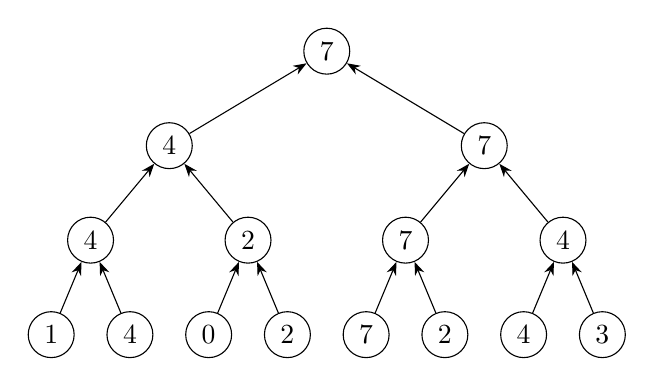
\begin{tikzpicture}
                        [level distance=12mm,
                         level 1/.style={sibling distance=40mm},
                         level 2/.style={sibling distance=20mm},
                         level 3/.style={sibling distance=10mm},
                         every node/.style={draw, circle, inner sep=3pt},
                         edge from parent/.style={draw, {Stealth}-}]

                        \node {7} % Root
                        child {node {4}
                            child {node {4}
                            child {node {1} }
                            child {node {4} }
                            }
                            child {node {2}
                            child {node {0} }
                            child {node {2} }
                            }
                        }
                        child {node {7}
                            child {node {7}
                            child {node {7} }
                            child {node {2} }
                            }
                            child {node {4}
                            child {node {4} }
                            child {node {3} }
                            }
                        };
                    \end{tikzpicture}
                \end{center}
                The comparison made are:
                \begin{enumerate}
                    \item Level 1:
                    \begin{itemize}
                        \item Pairs:
                        \begin{itemize}
                            \item \texttt{max(1, 4)}
                            \item \texttt{max(0, 2)}
                            \item \texttt{max(7, 2)}
                            \item \texttt{max(4, 3)}
                        \end{itemize}
                        \item Result: \texttt{[4, 2, 7, 4]}
                    \end{itemize}

                    \item Level 2:
                    \begin{itemize}
                        \item Pairs:
                        \begin{itemize}
                            \item \texttt{max(4, 2)}
                            \item \texttt{max(7, 4)}
                        \end{itemize}
                        \item Result: \texttt{[4, 7]}
                    \end{itemize}

                    \item Level 3:
                    \begin{itemize}
                        \item Pair: \texttt{max(4, 7)}
                        \item Result: \texttt{[7]}
                    \end{itemize}
                \end{enumerate}
                At this point, the Up-Sweep phase has found the maximum value of the entire array.
            \end{examplebox}

            \item \definitionWithSpecificIndex{Down-Sweep Phase}{Down-Sweep}{}. Use the partial results from the Up-Sweep phase to \textbf{compute the final scan results for all elements in the array}.
            \begin{enumerate}
                \item \textbf{Initialization}: \hl{Begin with an initial value, typically the identity element} (for maximum, it could be negative infinity $-\infty$).
                \item \textbf{Propagate Results}: \hl{Propagate the maximum values back down the tree}, updating the results for each element.
            \end{enumerate}
            \setcounter{example}{36}
            \begin{examplebox}[ (continue): Down-Sweep technique]
                Continuing from the Up-Sweep phase result \texttt{[7]} and the original array \texttt{[1, 4, 0, 2, 7, 2, 4, 3]} (page \hqpageref{example: Up-Sweep (Reduce) technique}).
                
                \highspace
                The main rule followed during the down-sweep technique is the following: the left leaf always inserts the value of the parent node, while the right leaf inserts the value calculated after applying the \texttt{max} operation to the value of the parent node and the left side just removed (which we find on the up-sweep graph).
                
                \highspace
                On the last level of the tree, there is an exception: before inserting the left leaf directly, the \texttt{max} operation of the inherited value and the input value must be performed.

                \highspace
                The steps are detailed:
                \begin{enumerate}
                    \item Replace the maximum value on the root (\texttt{7}) and insert the identity element, in our case the $-\infty$.
                    \begin{center}
                        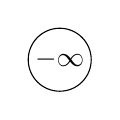
\begin{tikzpicture}
                            [level distance=14mm,
                             level 1/.style={sibling distance=40mm},
                             level 2/.style={sibling distance=20mm},
                             level 3/.style={sibling distance=10mm},
                             every node/.style={draw, circle, minimum size=8mm, inner sep=0pt},
                             edge from parent/.style={draw, -{Stealth}}]
    
                            \node {$-\infty$};
                        \end{tikzpicture}
                    \end{center}
                    \item Level 1:
                    \begin{itemize}
                        \item Insert the parent node on the left leaf, so $-\infty$.
                        \item On the right leaf, insert the performed operation between the parent's value and the left leaf of the up-sweep tree. So the values to compare are $-\infty$ and $4$: \texttt{max($-\infty$, 4) = 4}
                    \end{itemize}
                    \begin{center}
                        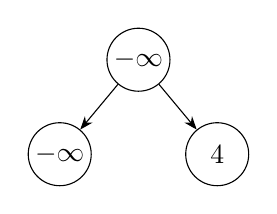
\begin{tikzpicture}
                            [level distance=12mm,
                             level 1/.style={sibling distance=20mm},
                             every node/.style={draw, circle, minimum size=8mm, inner sep=0pt},
                             edge from parent/.style={draw, -{Stealth}}]
    
                            \node {$-\infty$} % Root
                            child {node {$-\infty$}}
                            child {node {4}};
                        \end{tikzpicture}
                    \end{center}
                    \newpage
                    \item Level 2 ((from left to the right)):
                    \begin{itemize}
                        \item Vertex $-\infty$:
                        \begin{itemize}
                            \item Insert the parent node on the \textbf{left leaf}, so $-\infty$. It's not the last leaf of the tree, so we don't do any checking.

                            \item The \textbf{right leaf} comparison is between $-\infty$ (the father's value) and the left leaf on the up-sweep tree (the value just replaced by the $-\infty$), so 4. Again, the comparison is:
                            \begin{equation*}
                                \texttt{max($-\infty$, 4) = 4}
                            \end{equation*}
                        \end{itemize}

                        \item Vertex $4$:
                        \begin{itemize}
                            \item Insert the parent node on the \textbf{left leaf}, so $4$.
                            \item The \textbf{right leaf} comparison is between 4 (the father's value) and the left leaf on the up-sweep tree (the value just replaced by 4), so 7. The comparison is:
                            \begin{equation*}
                                \texttt{max(4, 7) = 7}
                            \end{equation*}
                        \end{itemize}
                    \end{itemize}
                    \begin{center}
                        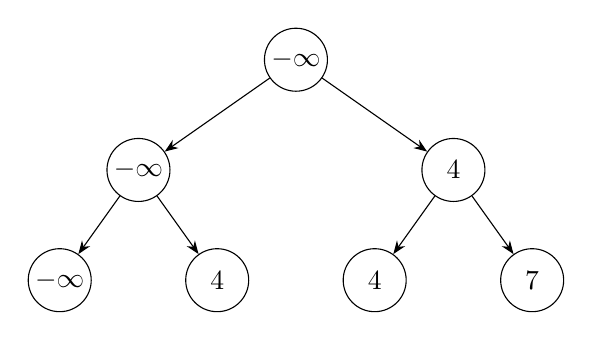
\begin{tikzpicture}
                            [level distance=14mm,
                             level 1/.style={sibling distance=40mm},
                             level 2/.style={sibling distance=20mm},
                             level 3/.style={sibling distance=10mm},
                             every node/.style={draw, circle, minimum size=8mm, inner sep=0pt},
                             edge from parent/.style={draw, -{Stealth}}]
    
                            \node {$-\infty$} % Root
                            child {node {$-\infty$}
                                child {node {$-\infty$}}
                                child {node {4}}
                            }
                            child {node {4}
                                child {node {4}}
                                child {node {7}}
                            };
                        \end{tikzpicture}
                    \end{center}
                    \item Level 3 (from left to the right):
                    \begin{itemize}
                        \item Vertex $-\infty$:
                        \begin{itemize}
                            \item \textbf{Left leaf}. Since this is the last level, we need to compute an extra check. We need to compute:
                            \begin{equation}
                                \texttt{max(inherited val, input val)}
                            \end{equation}\label{eq: down-sweep last level}
                            In our case, the inherited value is the $-\infty$, but the input value on the first position is 1. Therefore:
                            \begin{equation*}
                                \texttt{max($-\infty$, 1) = 1}
                            \end{equation*}
                            \item \textbf{Right leaf}. We compare the value we just removed, 1, to the value of the parent: $-\infty$.
                            \begin{equation*}
                                \texttt{max(1, $-\infty$) = 1}
                            \end{equation*}
                            The result should be 1 \underline{BUT} we are at the last level of the tree. So we need to do an extra check between the inherited value (what we want to place) and the input value on the second position (our case 4):
                            \begin{equation*}
                                \texttt{max(1, 4) = 4}
                            \end{equation*}
                        \end{itemize}
                        \item Vertex $4$:
                        \begin{itemize}
                            \item \textbf{Left leaf}. We apply formula \ref{eq: down-sweep last level} on page \pageref{eq: down-sweep last level}, the idea is the same as before:
                            \begin{equation*}
                                \texttt{max(4, 0) = 4}
                            \end{equation*}
                            \item \textbf{Right leaf}. We compare the value just removed, 0, to the value of parent: 4.
                            \begin{equation*}
                                \texttt{max(0, 4) = 4}
                            \end{equation*}
                            And the value obtained with the input value on the array:
                            \begin{equation*}
                                \texttt{max(4, 2) = 4}
                            \end{equation*}
                        \end{itemize}
                        \item Vertex $4$:
                        \begin{itemize}
                            \item \textbf{Left leaf}. We apply formula \ref{eq: down-sweep last level} on page \pageref{eq: down-sweep last level}, the idea is the same as before:
                            \begin{equation*}
                                \texttt{max(4, 7) = 7}
                            \end{equation*}
                            \item \textbf{Right leaf}. We compare the value just removed, 7, to the value of parent: 4.
                            \begin{equation*}
                                \texttt{max(7, 4) = 7}
                            \end{equation*}
                            And the value obtained with the input value on the array:
                            \begin{equation*}
                                \texttt{max(7, 2) = 7}
                            \end{equation*}
                        \end{itemize}
                        \newpage
                        \item Vertex $7$:
                        \begin{itemize}
                            \item \textbf{Left leaf}. We apply formula \ref{eq: down-sweep last level} on page \pageref{eq: down-sweep last level}, the idea is the same as before:
                            \begin{equation*}
                                \texttt{max(7, 4) = 7}
                            \end{equation*}
                            \item \textbf{Right leaf}. We compare the value just removed, 4, to the value of parent: 7.
                            \begin{equation*}
                                \texttt{max(4, 7) = 7}
                            \end{equation*}
                            And the value obtained with the input value on the array:
                            \begin{equation*}
                                \texttt{max(7, 3) = 7}
                            \end{equation*}
                        \end{itemize}
                    \end{itemize}
                    \begin{center}
                        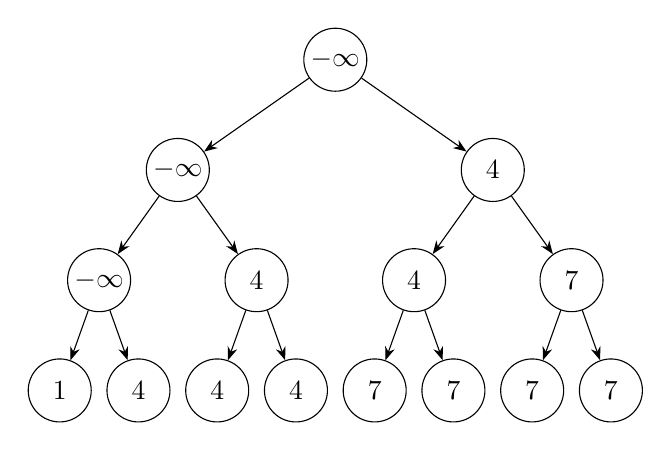
\begin{tikzpicture}
                            [level distance=14mm,
                             level 1/.style={sibling distance=40mm},
                             level 2/.style={sibling distance=20mm},
                             level 3/.style={sibling distance=10mm},
                             every node/.style={draw, circle, minimum size=8mm, inner sep=0pt},
                             edge from parent/.style={draw, -{Stealth}}]
    
                            \node {$-\infty$} % Root
                            child {node {$-\infty$}
                                child {node {$-\infty$}
                                child {node {1} }
                                child {node {4} }
                                }
                                child {node {4}
                                child {node {4} }
                                child {node {4} }
                                }
                            }
                            child {node {4}
                                child {node {4}
                                child {node {7} }
                                child {node {7} }
                                }
                                child {node {7}
                                child {node {7} }
                                child {node {7} }
                                }
                            };
                        \end{tikzpicture}
                    \end{center}
                \end{enumerate}
            \end{examplebox}
        \end{enumerate}
    \end{itemize}
    \begin{figure}[!htp]
        \centering
        \includegraphics[width=.85\textwidth]{img/maximum-up-down-sweep-1.pdf}
        \caption{Graphical example of the Maximum Algorithm with Up and Down Sweep. On the left a sequential version and on the right a parallel version. The parallel version was analyzed on the previous pages.}
    \end{figure}


    \item \definition{Three-Phase Scan with Tiling}
    \begin{itemize}
        \item[\textcolor{Red2}{\faIcon{book}}] \textcolor{Red2}{\textbf{Definition}}. Three-Phase Scan with Tiling is a technique that \textbf{divides the input array into smaller tiles and processes them in three distinct phases} to efficiently perform the scan operation.
        
        The main goal is to improve parallelism and cache efficiency by splitting the input array into smaller tiles and processing them independently.

        \item[\textcolor{Green3}{\faIcon{tools}}] \textcolor{Green3}{\textbf{Algorithm}}
        \begin{enumerate}
            \item \definition{Tiling and Local Scan}. Divide the input array into smaller tiles and perform the scan operation on each tile independently.
            \begin{enumerate}
                \item \textbf{Divide the Input Array}: Break the input array into smaller blocks or tiles.
                \item \textbf{Local Scan} (Inclusive): Compute the scan for each tile independently.
            \end{enumerate}
            \begin{examplebox}[: Tiling and Local Scan]
                For an array \texttt{[1, 2, 3, 4, 5, 6, 7, 8]} with a tile size of 4:
                \begin{itemize}
                    \item Tiles: \texttt{[1, 2, 3, 4]} and \texttt{[5, 6, 7, 8]}
                    \item Local Scans:
                    \begin{itemize}
                        \item First tile: \texttt{[1, 3, 6, 10]}
                        \item Second tile: \texttt{[5, 11, 18, 26]}
                    \end{itemize}
                \end{itemize}
            \end{examplebox}

            \item \definition{Scan of Tile Results}. Compute the \textbf{scan of the final elements of each tile to handle dependencies between tiles}.
            \begin{enumerate}
                \item \textbf{Extract Final Elements}: Take the last element of each tile.
                \item \textbf{Global Scan}: Perform a scan operation on these final elements to propagate the results across tiles.
            \end{enumerate}
            \begin{examplebox}[: Scan of Tile Results]
                \begin{itemize}
                    \item Final Elements: \texttt{10} (from the first tile) and \texttt{26} (from the second tile)
                    \item Global Scan: \texttt{[10, 36]} (assuming addition and identity element \texttt{0})
                \end{itemize}
            \end{examplebox}

            \item \definition{Distribution of Tile Results}. \textbf{Distribute the results of the scanned tile results to all elements in their respective tiles}.
            \begin{enumerate}
                \item \textbf{Distribute Results}: Add the scan results of the previous tiles to the elements of the current tile.
            \end{enumerate}
            \begin{examplebox}[: Distribution of Tile Results]
                \begin{itemize}
                    \item First Tile Remains the Same: \texttt{[1, 3, 6, 10]}
                    \item Second Tile: add the scan result \texttt{10} from the first tile's last element:
                    \begin{itemize}
                        \item \texttt{5 + 10 = 15}
                        \item \texttt{11 + 10 = 21}
                        \item \texttt{18 + 10 = 28}
                        \item \texttt{26 + 10 = 36}
                    \end{itemize}
                    \begin{equation*}
                        \texttt{[15, 21, 28, 36]}
                    \end{equation*}
                \end{itemize}
                Combining the results of the two tiles, we get:
                \begin{equation*}
                    \texttt{[1, 3, 6, 10, 15, 21, 28, 36]}
                \end{equation*}
            \end{examplebox}
        \end{enumerate}
    \end{itemize}
    \begin{figure}[!htp]
        \centering
        \includegraphics[width=\textwidth]{img/three-phase-scan-with-tiling-1.pdf}
        \caption{Graphical example of the Three-Phase Scan with Tiling.}
    \end{figure}


    \item \definition{Fusion of Map Pattern with Scan Pattern}
    \begin{itemize}
        \item[\textcolor{Red2}{\faIcon{book}}] \textcolor{Red2}{\textbf{Definition}}. Combine the transformation capabilities of the map pattern with the cumulative operations of the scan pattern to \textbf{achieve more complex and efficient parallel computations}.
        
        When we fuse the map and scan patterns, we \textbf{first apply the map function to transform each element in the input sequence}, and \textbf{then apply the scan operation to the transformed sequence}.

        \item[\textcolor{Green3}{\faIcon{tools}}] \textcolor{Green3}{\textbf{Algorithm}}
        \begin{enumerate}
            \item \textbf{Apply Map Function}: Transform each element in the input sequence using the map function.
            \item \textbf{Apply Scan Operation}: Perform the scan operation on the transformed sequence to compute cumulative results.
        \end{enumerate}
    \end{itemize}
    \begin{examplebox}[: Fusion of Map Pattern with Scan Pattern]
        Let's consider a practical example where we want to compute the prefix sums of the squares of an input array \texttt{[1, 2, 3, 4]}.
        \begin{enumerate}
            \item \textbf{Map Function}
            \begin{enumerate}
                \item Define the map function as $f\left(x\right) = x^{2}$.
                \item Apply the map function: \texttt{[1, 4, 9, 16]} (squares of the input elements),
            \end{enumerate}
            \item \textbf{Scan Operation}
            \begin{enumerate}
                \item Perform an inclusive scan on the transformed sequence \texttt{[1, 4, 9, 16]}.
                \item Inclusive scan result: \texttt{[1, 5, 14, 30]}.
            \end{enumerate}
        \end{enumerate}
    \end{examplebox}
    \begin{figure}[!htp]
        \centering
        \includegraphics[width=\textwidth]{img/fusion-map-with-scan-1.pdf}
        \caption{Graphical example of the Fusion of Map Pattern with Scan Pattern.}
    \end{figure}
\end{itemize}


    %%%%%%%%%%%%%%%%%%%%%%%%%%%%%%%%%%%%%%%%%%
    % Heterogeneous Computing - DSLs and HLS %
    %%%%%%%%%%%%%%%%%%%%%%%%%%%%%%%%%%%%%%%%%%
    \section{Heterogeneous Computing - DSLs and HLS}

\subsection{Introduction to Heterogeneous Computing}

\definition{Heterogeneous Computing} (or \definition{Heterogeneous Processing}) refers to \textbf{systems that use multiple types of processors or accelerators to handle different workloads more efficiently}.
\begin{itemize}
    \item In contrast to traditional homogeneous systems (which only use CPUs), heterogeneous systems combine different processing units such as CPUs, GPUs, DSPs, and FPGAs.
    \item The \textbf{goal is to match the right processor to the right task},  achieving higher performance and energy efficiency.  
\end{itemize}

\begin{examplebox}[: Heterogeneous Processing]
    A self-driving car requires CPUs for decision-making, GPUs for image recognition, and FPGAs for real-time sensor fusion.
\end{examplebox}

\highspace
\begin{flushleft}
    \textcolor{Green3}{\faIcon{\speedIcon} \textbf{Energy-Efficient Computing Strategies}}
\end{flushleft}
When designing a heterogeneous system, performance isn't the only goal; \textbf{energy efficiency is just as critical}. Given a fixed power budget, simply \textbf{increasing performance without considering power constraints is inefficient}. Specialized hardware (e.g., FPGAs, ASICs) achieves better performance per watt than general-purpose processors.

\highspace
There are two main strategies for improving energy efficiency:
\begin{enumerate}
    \item \important{Use Specialized Processors}. \textbf{CPUs are not energy-efficient} due to instruction decoding, branch handling, and pipeline management overhead. Specialized hardware (FPGAs, ASICs) reduces overhead, leading to more computations per joule.
    \begin{equation*}
        \text{Power} = \dfrac{\text{Op}}{\text{second}} \times \dfrac{\text{Joules}}{\text{Op}}
    \end{equation*} 
    \item \important{Minimize Data Movement}. \textbf{Memory access consumes more energy than computation!} Optimizing data locality reduces power consumption. For example, moving computation closer to memory (e.g., using tensor core inside GPUs) significantly reduces energy cost.
\end{enumerate}

    \subsection{Heterogeneous parallel programming}

\begin{flushleft}
    \textcolor{Red2}{\faIcon{exclamation-triangle} \textbf{Challenges of Writing Portable and Efficient Parallel Code}}
\end{flushleft}
Writing parallel programs for heterogeneous systems is difficult due to the following reasons:
\begin{enumerate}
    \item \important{Diverse Hardware Architectures}. A CPU, GPU, and FPGA all have different programming models. \textbf{Code written for one hardware type may not perform well on another}.
    
    \item \important{Performance vs. Productivity Trade-offs}.
    \begin{itemize}
        \item \textbf{Performance}: Low-level programming (e.g., \hl{CUDA, OpenCL, Verilog}) allows fine-tuned optimizations but \textbf{is hard to program}.
        \item \textbf{Productivity}: High-level abstractions (e.g., \hl{OpenMP, DSLs}) improve productivity but \textbf{may introduce performance overhead}.
    \end{itemize}

    \item \important{Memory Management}. Different memory models (shared vs. distributed) require different optimizations. Data movement between CPU and GPU memory can be costly if not handled efficiently.

    \item \important{Scalability Issues}. Some \textbf{programs scale well on GPUs but poorly on CPUs} due to synchronization and memory bandwidth limitations.
\end{enumerate}

\begin{flushleft}
    \textcolor{Green3}{\faIcon{check-circle} \textbf{The Ideal Parallel Programming Language}}
\end{flushleft}
An \textbf{ideal parallel programming model should provide a balance of}:
\begin{itemize}[label=\textcolor{Green3}{\faIcon{check}}]
    \item \textcolor{Green3}{\textbf{Performance}}. Optimized execution across different hardware.
    \item \textcolor{Green3}{\textbf{Productivity}}. Easy to use and develop.
    \item \textcolor{Green3}{\textbf{Generality}}. Works across different architectures.
\end{itemize}
However, \textbf{most existing languages optimize only one or two} of these factors, leading to trade-offs.

\begin{table}[!htp]
    \centering
    \begin{tabular}{@{} p{12em} | c c c @{}}
        \toprule
        \textbf{Approach} & \textbf{Performance} & \textbf{Productivity} & \textbf{Generality} \\
        \midrule
        \textbf{CUDA/OpenCL}            & \textcolor{Green3}{\faIcon{check} \textbf{High}}      & \textcolor{Red2}{\faIcon{times} \textbf{Low}}         & \textcolor{Red2}{\faIcon{times} \textbf{Low}} \\ [.5em]
        \textbf{OpenMP (CPU)}           & \textcolor{Green3}{\faIcon{check} \textbf{High}}      & \textcolor{Green3}{\faIcon{check} \textbf{Medium}}    & \textcolor{Red2}{\faIcon{times} \textbf{Low}} \\ [.5em]
        \textbf{MPI (Distributed)}      & \textcolor{Green3}{\faIcon{check} \textbf{High}}      & \textcolor{Red2}{\faIcon{times} \textbf{Low}}         & \textcolor{Green3}{\faIcon{check} \textbf{High}} \\ [.5em]
        \textbf{FPGA/Verilog/VHDL}      & \textcolor{Green3}{\faIcon{check} \textbf{Very High}} & \textcolor{Red2}{\faIcon{times} \textbf{Very Low}}    & \textcolor{Red2}{\faIcon{times} \textbf{Low}} \\ [.5em]
        \textbf{High-Level Synthesis}   & \textcolor{Green3}{\faIcon{check} \textbf{High}}      & \textcolor{Green3}{\faIcon{check} \textbf{Medium}}    & \textcolor{Red2}{\faIcon{times} \textbf{Low}} \\
        \bottomrule
    \end{tabular}
\end{table}

\highspace
\begin{flushleft}
    \textcolor{Green3}{\faIcon{question-circle} \textbf{Why is this important?}}
\end{flushleft}
If we want \textbf{portable parallel programs}, we need \textbf{new high-level abstractions} like Domain-Specific Languages (DSLs), which will be covered in the next section.
    \subsection{DSLs and Halide}

\begin{flushleft}
    \textcolor{Green3}{\faIcon{question-circle} \textbf{What are Domain-Specific Languages (DSLs)?}}
\end{flushleft}
A \definition{Domain-Specific Language (DSL)} is a \textbf{specialized programming language} designed for a \textbf{specific application domain}. The main characteristics of DSLs are:
\begin{itemize}
    \item \important{Restricted expressiveness} (focused on a single domain)
    \item \important{High-level, declarative syntax} (easier than general purpose languages)
    \item \important{Optimized performance} for the target domain
    \item \important{May be standalone or embedded} in another language
\end{itemize}

\begin{table}[!htp]
    \centering
    \begin{tabular}{@{} l l p{16em} @{}}
        \toprule
        \textbf{DSL Name} & \textbf{Target Domain} & \textbf{Key Benefits} \\
        \midrule
        \textbf{Halide}       & Image Processing   & Separates algorithm from scheduling for optimized execution. \\ [.5em]
        \textbf{TensorFlow}   & Machine Learning   & Optimized computation graphs for AI workloads. \\ [.5em]
        \textbf{SQL}          & Databases          & Declarative queries for efficient data retrieval. \\ [.5em]
        \textbf{Verilog/VHDL} & Hardware Design    & Describes digital circuits for synthesis. \\
        \bottomrule
    \end{tabular}
    \caption{Examples of DSLs.}
\end{table}

\highspace
\begin{flushleft}
    \textcolor{Green3}{\faIcon{balance-scale} \textbf{Embedded vs. External DSLs}}
\end{flushleft}
DSLs can be classified as:
\begin{itemize}
   \item \important{External} DSLs:
   \begin{itemize}
      \item[\textcolor{Red2}{\faIcon{book}}] Have \textbf{their own} \emph{syntax} and \emph{compiler}/\emph{interpreter}.
      \item[\textcolor{Green3}{\faIcon{question-circle}}] \example{Example}: SQL, Halide, Verilog.
      \item[\textcolor{Green3}{\faIcon{check-circle}}] \textcolor{Green3}{\textbf{Advantages}}: can be \textbf{more optimized} but require custom compilers.
   \end{itemize}
   \item \important{Embedded} DSLs:
   \begin{itemize}
      \item[\textcolor{Red2}{\faIcon{book}}] \textbf{Built inside another general-purpose language}.
      \item[\textcolor{Green3}{\faIcon{question-circle}}] \example{Example}: TensorFlow (embedded in Python).
      \item[\textcolor{Green3}{\faIcon{check-circle}}] \textcolor{Green3}{\textbf{Advantages}}: benefit from \textbf{integration} with the host language
   \end{itemize}
\end{itemize}

\newpage

\begin{flushleft}
   \textcolor{Green3}{\faIcon{bolt} \textbf{DSL Use Case: Halide for Image Processing}}
\end{flushleft}
\definition{Halide} is a \textbf{Domain-Specific Language (DSL) for high-performance image processing}. 
\begin{itemize}
   \item[\textcolor{Green3}{\faIcon{question-circle}}] \textcolor{Green3}{\textbf{Why does image processing need DSLs?}}
   \begin{itemize}
      \item[\textcolor{Green3}{\faIcon{\speedIcon}}] Image processing is \textbf{data-intensive} and \hl{requires high performance}.
      \item[\textcolor{Red2}{\faIcon{thumbs-down}}] \hl{Traditional solutions} (\texttt{C++}, \texttt{CUDA}, \texttt{OpenCV}) \hl{require manual optimizations}.
      \item[\textcolor{Red2}{\faIcon{frown}}] Optimizing code for \textbf{parallelism and memory efficiency} is \textbf{difficult}.
   \end{itemize}

   \item[\textcolor{Green3}{\faIcon{question-circle}}] \textcolor{Green3}{\textbf{Why Halide?}}
   \begin{itemize}
      \item[\textcolor{Green3}{\faIcon{cut}}] \textbf{Separates ``\emph{what}'' is computed from ``\emph{how}'' it is executed}.
      \item[\textcolor{Green3}{\faIcon{code}}] \textbf{Expresses computations at a high level}, leaving optimizations to the compiler.
      \item[\textcolor{Green3}{\faIcon{globe}}] \textbf{Portable} across CPUs, GPUs, and FPGAs.
   \end{itemize}
\end{itemize}

\highspace
\begin{flushleft}
   \textcolor{Green3}{\faIcon{tools} \textbf{How Halide Works: Separating Algorithm from Schedule}}
\end{flushleft}
In Halide, a \textbf{key feature is the separation} of \textbf{what} a program computes (\emph{computation}/\emph{algorithm}) from \textbf{how} it executes (\emph{schedule}). This means:
\begin{itemize}
   \item The \important{algorithm} specifies \textbf{what operations should be performed}. In other words, specifies \textbf{what to compute} (like a mathematical formula).
   \item The \important{schedule} defines \textbf{how those operations should be executed efficiently} on the hardware. In other words, specifies \textbf{how to execute the computation} (parallelism, memory layout, vectorization).
\end{itemize}
Now we see the difference between the traditional approach we have always used and the halide approach:
\begin{itemize}
   \item \important{Traditional Approach (\texttt{C++}, \texttt{CUDA}, \texttt{OpenCV})}. In traditional programming languages (e.g., \texttt{C++}, \texttt{OpenCV}, \texttt{CUDA}), the \textbf{algorithm and execution strategy are mixed together}. This means that if we want to \textbf{change parallelization or memory access optimizations}, we must \textbf{rewrite parts of the algorithm itself}. This makes it \emph{hard to experiment} with different optimizations.

   \begin{flushleft}
      \textcolor{Red2}{\faIcon{exclamation-triangle} \textbf{Problems with the Traditional Approach}}
   \end{flushleft}
   \begin{enumerate}
      \item \textbf{If we want to optimize} for vectorization, parallel execution, or memory layout, we \textbf{\hl{must modify the algorithm itself}}.
      \item The \textbf{\hl{same code cannot easily be reused}} for different architectures (e.g., CPU, GPU, FPGA).
   \end{enumerate}

   \begin{examplebox}[: Problems with the Traditional Approach]
      \begin{lstlisting}[language=c++]
void box_blur(const Image &in, Image &out) {
    for (int y = 1; y < in.height() - 1; y++) {
        for (int x = 1; x < in.width() - 1; x++) {
            out(x, y) = (
                in(x-1, y) + in(x, y) + in(x+1, y)
            ) / 3;
        }
    }
}\end{lstlisting}
      The problem here is that we need to specify the ``\emph{what}'', i.e. what operations should be performed, but also ``\emph{how}'' these operations should be performed.
   \end{examplebox}


   \item \important{Halide's Approach: Separate Algorithm from Execution}. Halide splits the computation into two parts:
   \begin{enumerate}
      \item \textbf{Computation} (Algorithm) - \emph{What to Compute}
      \begin{itemize}
         \item Defines the mathematical computation.
         \item \hl{Remains unchanged across different hardware targets}.
      \end{itemize}
      \item \textbf{Schedule} - \emph{How to Execute Efficiently}
      \begin{itemize}
         \item Controls memory layout, parallelization, and optimization.
         \item \hl{Can be changed without modifying the algorithm}.
      \end{itemize}
   \end{enumerate}

   \begin{examplebox}[: Box Blur in Halide]
      The computation part is separated from the scheduling!
      So a change in the algorithm can be made without affecting the control of the execution.
      Therefore, we define simply:
      \begin{enumerate}
         \item Computation (Algorithm), stays the same:
         \begin{lstlisting}[language=c++]
Var x, y;
Func blurx, blury;

// First pass: horizontal blur
blurx(x, y) = (in(x-1, y) + in(x, y) + in(x+1, y)) / 3;

// Second pass: vertical blur
blury(x, y) = (blurx(x, y-1) + blurx(x, y) + blurx(x, y+1)) / 3;\end{lstlisting}
         This part \textbf{only describes the math}, \textbf{\underline{not how}} it should run.
      
         \item Schedule, controls execution (can be changed easily):
         \begin{lstlisting}[language=c++]
blury.tile(x, y, xi, yi, 256, 32)
    // Vectorized execution for SIMD
    .vectorize(xi, 8)
    // Parallel execution over y-dimension
    .parallel(y);

blurx.compute_at(blury, x)  // Compute blurx only when needed by blury
    .vectorize(x, 8);\end{lstlisting}
         This part \textbf{controls execution strategy} but does \textbf{\underline{not} \underline{modify} the algorithm}.
         The \textbf{same algorithm} can now \textbf{run efficiently on different hardware architectures} just by changing the schedule.
      \end{enumerate}
   \end{examplebox}
\end{itemize}

\highspace
\begin{flushleft}
   \textcolor{Green3}{\faIcon{check-circle} \textbf{Why DSLs Matter for Performance and Productivity: Advantages}}
\end{flushleft}
\begin{itemize}[label=\textcolor{Green3}{\faIcon{check}}]
   \item \textcolor{Green3}{\textbf{Performance Optimization}}. A Halide program \textbf{can be better than hand-optimization \texttt{C++} code}. Scheduling decisions affect \textbf{parallel execution, memory locality, and vectorization}.
   \item \textcolor{Green3}{\textbf{Productivity}}. Instead of manually optimizing, \textbf{Halide allows rapid exploration of different schedules}. Easier to \textbf{port to different architectures} (CPU, GPU, FPGA).
\end{itemize}
In conclusion, DSLs like Halide \textbf{automate low-level optimizations}, enabling \emph{faster} and \emph{more efficient} code for specialized domains.

    \subsection{Scheduling \& Performance Optimization in Halide}

This section focuses on \textbf{how different scheduling strategies in Halide affect performance} and how to \textbf{choose the best schedule for different hardware architectures}.

\highspace
\begin{flushleft}
    \textcolor{Green3}{\faIcon{question-circle} \textbf{Why Scheduling Matters}}
\end{flushleft}
Scheduling is the \textbf{key to optimizing performance in Halide}.
\begin{itemize}
    \item A \textbf{poorly scheduled program can be $10\times$ slower than an optimized one}.
    \item \textbf{Memory access, cache locality, parallelism, and vectorization} all \hl{depend on scheduling}.
\end{itemize}
As we have already seen, in traditional languages (C++, CUDA, OpenMP), scheduling decisions must be hard-coded into the algorithm. In Halide, the schedule is separate and can be changed without changing the algorithm.

\highspace
\begin{flushleft}
    \textcolor{Green3}{\faIcon{question-circle} \textbf{How Scheduling Affects Performance}}
\end{flushleft}
Different \textbf{scheduling strategies} impact how the computation is executed on hardware:
\begin{table}[!htp]
    \centering
    \begin{tabular}{@{} l p{20em} @{}}
        \toprule
        \textbf{Scheduling Strategy} & \textbf{Impact} \\
        \midrule
        \textbf{Serial Execution} & Simple, but slow. No parallelism. \\ [.5em]
        \textbf{Parallel Execution} & Uses multiple CPU cores. Good for multi-core CPUs. \\ [.5em]
        \textbf{Vectorization (SIMD)} & Uses wide registers for efficiency (e.g., AVX). \\ [.5em]
        \textbf{Tiling} & Improves cache locality by processing data in chunks. \\ [.5em]
        \textbf{Compute-at} & Controls when intermediate results are com-\break puted. \\ [.5em]
        \textbf{Store-at} & Controls where intermediate results are stored. \\
        \bottomrule
    \end{tabular}
\end{table}

\highspace
\begin{flushleft}
    \textcolor{Green3}{\faIcon{tasks} \textbf{Scheduling Strategies in Halide}}
\end{flushleft}
Let's take the Box Blur Algorithm as an example. The \definition{Box Blur} is a simple \textbf{image processing technique used for smoothing or blurring an image}. It performs two main steps:
\begin{enumerate}
    \item \textbf{Each pixel} in the output image is computed as the \textbf{average of its neighboring pixels}.
    \item It applies a \textbf{moving average filter} over a \textbf{small window} (e.g., $3 \times 3$ or $5 \times 5$ pixels).
\end{enumerate}
It is used to reduce noise in images, to create a smooth, blurry effect and, above all, because it is fast and efficient, since it involves only two operations: adding and dividing.

\highspace
However, we will now analyze the algorithm implemented in Halide using different strategies:
\begin{itemize}
    \item[\textcolor{Red2}{\faIcon{hourglass-half}}] \textcolor{Red2}{\textbf{Default Serial Execution (Slow)}}. Without scheduling, Halide will execute in \textbf{serial order} (one pixel at a time).
    \begin{lstlisting}[language=c++]
Var x, y;
Func blurx, blury;

blurx(x, y) = (in(x-1, y) + in(x, y) + in(x+1, y)) / 3;
blury(x, y) = (blurx(x, y-1) + blurx(x, y) + blurx(x, y+1)) / 3;\end{lstlisting}
    \begin{flushleft}
        \textcolor{Red2}{\faIcon{times-circle} \textbf{Problems}}
    \end{flushleft}
    \begin{itemize}[label=\textcolor{Red2}{\faIcon{times}}]
        \item No parallelism or vectorization.
        \item Poor memory access patterns.
        \item Slow execution.
    \end{itemize}


    \item[\textcolor{Red2}{\faIcon{\speedIcon}}] \textcolor{Red2}{\textbf{Parallel Execution}}. We can \textbf{add parallelism} to use multiple CPU cores:
    \begin{lstlisting}[language=c++]
blury.parallel(y);\end{lstlisting}
    
    \begin{flushleft}
        \textcolor{Green3}{\faIcon{check-circle} \textbf{Advantages}}
    \end{flushleft}
    \begin{itemize}[label=\textcolor{Green3}{\faIcon{check}}]
        \item \hl{Halide automatically splits the work across CPU cores}.
        \item Useful for multi-threaded execution on CPUs.
    \end{itemize}

    
    \item[\textcolor{Red2}{\faIcon{\speedIcon}}] \textcolor{Red2}{\textbf{Vectorization (SIMD)}}. Modern CPUs support \textbf{SIMD instructions} (e.g., AVX, NEON) to process multiple pixels at once:
    \begin{lstlisting}[language=c++]
blury.vectorize(x, 8);\end{lstlisting}

    \begin{flushleft}
        \textcolor{Green3}{\faIcon{check-circle} \textbf{Advantages}}
    \end{flushleft}
    \begin{itemize}[label=\textcolor{Green3}{\faIcon{check}}]
        \item Uses \textbf{SIMD registers} for faster execution.
        \item Works best for \textbf{data-parallel workloads} like image processing.
    \end{itemize}


    \item[\textcolor{Red2}{\faIcon{\speedIcon}}] \textcolor{Red2}{\textbf{Tiling for Better Cache Performance}}. Instead of processing the whole image at once, we \textbf{divide it into smaller tiles}:
    \begin{lstlisting}[language=c++]
blury.tile(x, y, xi, yi, 256, 32);\end{lstlisting}

    \begin{flushleft}
        \textcolor{Green3}{\faIcon{check-circle} \textbf{Advantages}}
    \end{flushleft}
    \begin{itemize}[label=\textcolor{Green3}{\faIcon{check}}]
        \item \textbf{Each tile fits better in cache}, \hl{reducing memory latency}.
        \item \textbf{Improves locality of reference} (\hl{less cache thrashing}).
    \end{itemize}


    \item[\textcolor{Red2}{\faIcon{\speedIcon}}] \textcolor{Red2}{\textbf{Optimized Schedule: Combining Techniques}}. We can \textbf{combine multiple scheduling strategies} for maximum performance:
    \begin{lstlisting}[language=c++]
// Process in 256x32 tiles
blury.tile(x, y, xi, yi, 256, 32)
    // Vectorized execution
    .vectorize(xi, 8)
    // Parallel execution across CPU cores
    .parallel(y);

// Compute blurx only when needed
blurx.compute_at(blury, x)
    .vectorize(x, 8);\end{lstlisting}

    \begin{flushleft}
        \textcolor{Green3}{\faIcon{check-circle} \textbf{Advantages}}
    \end{flushleft}
    \begin{itemize}[label=\textcolor{Green3}{\faIcon{check}}]
        \item Breaks image into \hl{tiles for cache efficiency}.
        \item Uses \hl{SIMD vectorization} for fast execution.
        \item \hl{Runs in parallel} on multiple CPU cores.
        \item Intermediate results (\texttt{blurx}) are \hl{computed only when needed}.
    \end{itemize}
\end{itemize}

\highspace
\begin{flushleft}
    \textcolor{Green3}{\faIcon{balance-scale} \textbf{Trade-offs in Scheduling}}
\end{flushleft}
But \emph{how do we choose the right scheduling?} Well, we need to find a good trade-off.
Different scheduling choices affect \textbf{performance trade-offs}:
\begin{table}[!htp]
    \centering
    \begin{tabular}{@{} l p{20em} @{}}
        \toprule
        \textbf{Scheduling Strategy} & \textbf{Performance Impact} \\
        \midrule
        \textbf{Parallel Execution} & Increases throughput, uses multiple cores. \\
        \textbf{Vectorization (SIMD)} & Improves performance on CPUs/GPUs. \\
        \textbf{Tiling} & Improves cache locality, reduces memory overhead. \\
        \textbf{Compute-at} & Avoids redundant computations. \\
        \textbf{Store-at} & Reduces memory footprint but increases recomputation. \\
        \bottomrule
    \end{tabular}
    \caption{Performance trade-offs in Scheduling.}
\end{table}

\highspace
\begin{flushleft}
    \textcolor{Green3}{\faIcon{check} \textbf{Conclusion}}
\end{flushleft}
In conclusion, the key takeaways are:
\begin{itemize}
    \item \textbf{Scheduling} is the \textbf{key to performance} in Halide.
    \item \textbf{Parallel execution}, \textbf{vectorization}, and \textbf{tiling} significantly \hl{improve performance}.
    \item \textbf{Halide's flexibility} allows \textbf{quick} experimentation with \textbf{different} \textbf{schedules}.
    \item The \textbf{right schedule depends on hardware constraints} (CPU, GPU, FPGA).
\end{itemize}
    \subsection{Introduction to HLS}

\begin{flushleft}
    \textcolor{Green3}{\faIcon{question-circle} \textbf{What is High-Level Synthesis (HLS)?}}
\end{flushleft}
\definition{High-Level Synthesis (HLS)} is a \textbf{process that converts high-level software code} (\texttt{C}/\texttt{C++}/\texttt{Python}) \textbf{into hardware designs} (Verilog/VHDL). It \textbf{automates hardware generation}, allowing developers to describe behavior in software-like code while the tool generates optimized circuits.

\highspace
\begin{flushleft}
    \textcolor{Red2}{\faIcon{book} \textbf{Traditional FPGA/ASIC Design Flow (Without HLS)}}
\end{flushleft}
The traditional FPGA or ASIC design flow is divided into three main steps:
\begin{enumerate}
    \item \textbf{Write Register-Transfer Level (RTL) code} in Verilog/VHDL.
    \item Manually optimize for \textbf{timing, area, power}.
    \item Run \textbf{logic synthesis}, \textbf{place \& route}, and \textbf{fabrication}.
\end{enumerate}
The main \textbf{problems} with this approach are:
\begin{itemize}[label=\textcolor{Red2}{\faIcon{times}}]
    \item \textcolor{Red2}{\textbf{Time-consuming}} (designing hardware manually takes months).
    \item \textcolor{Red2}{\textbf{Error-prone}} (low-level bugs are hard to debug).
    \item \textcolor{Red2}{\textbf{Difficult to modify}} (small changes require rewriting RTL code).
\end{itemize}

\begin{table}[!htp]
    \centering
    \begin{tabular}{@{} l p{11.3em} p{11.3em} @{}}
        \toprule
        \textbf{Aspect} & \textbf{Traditional RTL} & \textbf{High-Level Synthesis} \\
        \midrule
        \textbf{Design Level} & Low-level: gates, registers & High-level (\texttt{C++}, \texttt{Python}) \\ [.7em]
        \textbf{Productivity} & \textcolor{Red2}{\faIcon{times}} Time-consuming & \textcolor{Green3}{\faIcon{check}} Faster development \\ [.7em]
        \textbf{Optimizations} & Manual pipeline and control logic & Automated scheduling \\ [.7em]
        \textbf{Reusability} & \textcolor{Red2}{\faIcon{times}} Difficult to modify & \textcolor{Green3}{\faIcon{check}} Easily reusable code \\ [.7em]
        \textbf{Learning Curve} & Steep (hardware expertise needed) & Easier (similar to software programming) \\
        \bottomrule
    \end{tabular}
    \caption{\textcolor{Green3}{\faIcon{balance-scale}} Differences Between HLS and RTL-Based Hardware Design.}
\end{table}

\noindent
We can conclude that \textbf{HLS allows software engineers to efficiently design hardware without deep knowledge of Verilog/VHDL}.

\newpage

\begin{flushleft}
    \textcolor{Green3}{\faIcon{check-circle} \textbf{Why use HLS instead of traditional RTL design? Benefits of HLS}}
\end{flushleft}
\begin{enumerate}[label=\textcolor{Green3}{\faIcon{check}}]
    \item \textcolor{Green3}{\textbf{Faster Development Cycle}}. \textbf{Designers can write \texttt{C++}/\texttt{Python} instead of Verilog}, reducing design time.
    \item \textcolor{Green3}{\textbf{Automated Optimizations}}. \textbf{HLS compilers automatically optimize} \hl{parallelism}, \hl{pipelining}, and \hl{resource allocation}.
    \item \textcolor{Green3}{\textbf{Easier HW/SW Co-Design}}. Enables \textbf{rapid prototyping of hardware accelerators}.
    \item \textcolor{Green3}{\textbf{Technology Independence}}. The \textbf{same \texttt{C++} code can be compiled for different FPGA/ASIC platforms}.
\end{enumerate}

\highspace
\begin{flushleft}
    \textcolor{Red2}{\faIcon{times-circle} \textbf{Challenges of HLS}}
\end{flushleft}
\begin{itemize}
    \item \textbf{Not all software code can be efficiently translated into hardware}.
    \item \textbf{HLS tools must explore a huge design space} (parallelism, pipelining, resource constraints).
    \item \textbf{Requires careful optimization of memory access and data flow}.
\end{itemize}

\highspace
\begin{flushleft}
    \textcolor{Green3}{\faIcon{check} \textbf{Conclusion}}
\end{flushleft}
In conclusion, the key takeaways are:
\begin{itemize}
    \item HLS \textbf{translates high-level software} (\texttt{C}/\texttt{C++}/\texttt{Python}) \textbf{into hardware designs} (Verilog/VHDL).
    \item It automates the hardware design process, \textbf{reducing time and complexity}.
    \item HLS enables software engineers to \textbf{design hardware accelerators without deep RTL expertise}.
    \item Challenges include \textbf{optimizing memory access, parallelism, and\break scheduling}.
\end{itemize}
    \subsection{HLS Workflow}

This section explains \textbf{\emph{how} HLS converts high-level code} (\texttt{C}/\texttt{C++}/\texttt{Python}) \textbf{into hardware} (Verilog/VHDL) and the key steps in the HLS design flow.

\highspace
\begin{flushleft}
    \textcolor{Green3}{\faIcon{keyboard} \textbf{Inputs to an HLS Compiler}}
\end{flushleft}
To generate hardware from high-level code, an \textbf{HLS tool requires three main inputs}:
\begin{enumerate}
    \item \important{High-Level Code} (\texttt{C}, \texttt{C++}, or \texttt{Python})
    \begin{itemize}
        \item Describes the \textbf{algorithm's behavior}.
        \item Written similarly to software but \textbf{optimized for hardware}.
    \end{itemize}
    \item \important{Library of Characterized Modules}
    \begin{itemize}
        \item \textbf{Predefined hardware} building blocks (e.g., adders, multipliers, memory units).
        \item Helps the compiler understand available resources.
    \end{itemize}
    \item \important{Constraints \& Optimization Directives}
    \begin{itemize}
        \item Designer-defined constraints such as:
        \begin{itemize}
            \item \textbf{Area constraints} (how much hardware can be used).
            \item \textbf{Timing constraints} (desired clock speed).
            \item \textbf{Memory hierarchy} (external vs. on-chip memory).
        \end{itemize}
        \item Optional \textbf{HLS pragmas} (e.g., loop unrolling, pipelining) to fine-tune performance.
    \end{itemize}
\end{enumerate}

\highspace
\begin{flushleft}
    \textcolor{Green3}{\faIcon{question-circle} \textbf{HLS Objectives}}
\end{flushleft}
The goal of \textbf{HLS is to generate an efficient hardware design} based on the following objectives:
\begin{itemize}[label=\textcolor{Green3}{\faIcon{check}}]
    \item \textcolor{Green3}{\textbf{Minimize Area}}: Uses fewer functional units, registers, and interconnects.
    \item \textcolor{Green3}{\textbf{Maximize Speed}}: Reduces the number of clock cycles (latency) and increases throughput.
    \item \textcolor{Green3}{\textbf{Optimize Power}}: Reduces energy consumption for embedded systems.
\end{itemize}
However, the main trade-offs must be:
\begin{itemize}
    \item \textbf{Optimizing for speed} $\Rightarrow$ may increase hardware area.
    \item \textbf{Reducing hardware area} $\Rightarrow$ may increase execution time.
\end{itemize}

\newpage

\begin{flushleft}
    \textcolor{Green3}{\faIcon{microchip} \textbf{HLS Compilation Flow}}
\end{flushleft}
HLS follows \textbf{three main steps}:
\begin{itemize}
    \item \important{Front-End (Parsing and IR Generation)}. \textbf{Converts} \texttt{C++}/\texttt{Python} \textbf{code} into an \definition{Intermediate Representation (IR)}. IR is \textbf{similar to software compiler representations} (e.g., LLVM IR). In other words, it breaks the program down into basic operations.
    
    \item \important{Middle-End (Optimization and Scheduling)}. At this point, the HLS tools performed three important operations:
    \begin{enumerate}
        \item It \textbf{analyzes data dependencies} and \textbf{determines execution order}.
        \item It performs \textbf{scheduling} (decides when each operation runs).
        \item It allocates \textbf{hardware resources} (multipliers, memory, registers).
    \end{enumerate}
    \begin{examplebox}[: Scheduling Choices]
        \begin{center}
            \begin{tabular}{@{} l p{15em} @{}}
                \toprule
                \textbf{Scheduling Strategy} & \textbf{Impact} \\
                \midrule
                \textbf{As Soon As Possible} & Minimizes latency, but may use more hardware. \\ [.5em]
                \textbf{As Late As Possible} & Reduces hardware usage, but may increase delay. \\ [.5em]
                \textbf{Loop Unrolling}      & Increases parallelism, but requires more area. \\ [.5em]
                \textbf{Pipelining}          & Allows overlapping computations to improve throughput. \\
                \bottomrule
            \end{tabular}
        \end{center}
    \end{examplebox}

    \item \important{Back-End (Hardware Generation)}. Finally, the tools made two steps:
    \begin{enumerate}
        \item \textbf{Converts optimized IR into Verilog/VHDL}.
        \item \textbf{Generates a Finite State Machine with Datapath (FSMD)} representation.
    \end{enumerate}
    The result is a \textbf{synthesizable hardware description} ready for FPGA/ASIC implementation.

    Therefore, a \textbf{final output} of HLS tools is:
    \begin{itemize}
        \item Verilog/VHDL code (for FPGA/ASIC synthesis).
        \item Datapath and Controller Design.
        \item Simulation files for verification.
    \end{itemize}
\end{itemize}

\newpage

\begin{flushleft}
    \textcolor{Green3}{\faIcon{check} \textbf{Conclusion}}
\end{flushleft}
In conclusion, the key takeaways are:
\begin{itemize}
    \item \textbf{HLS automates hardware design} from high-level code (\texttt{C}/\texttt{C++}/\texttt{Python}).
    \item The workflow involves \textbf{parsing}, \textbf{optimization}, \textbf{scheduling}, and \textbf{hardware generation}.
    \item \textbf{Performance tuning} requires adjusting \textbf{scheduling}, \textbf{pipelining}, and \textbf{parallelism}.
    \item \textbf{HLS outputs Verilog/VHDL}, which can be synthesized on FPGAs/ASICs.
\end{itemize}


    % TODO:
    % 3. Patterns:
    % 3.1 A (done)
    % 3.2 B (done)
    % 3.3 C (done)
    % 3.4 Stencil (from page 56) (done)
    % 4. Parallel patterns in OpenMP and CUDA (done)
    % 5. DSL - HLS
    %   - "Traditional" FPGA/ASIC design flow
    %   - High-Level Synthesis (HLS) p. 41-47
    %   - The FSMD model p. 48
    %   - Manual example p. 49-51
    %   - HLS IR basic concepts p. 52-54
    %   - HLS scheduling p. 55-72

    %%%%%%%%%%%%%%%%%%%%%%%%%%
    % Bibliography and index %
    %%%%%%%%%%%%%%%%%%%%%%%%%%
    \pagestyle{fancy}
\fancyhead{} % clear all header fields
\fancyhead[R]{\nouppercase{\leftmark\hfill\rightmark}}

\pagestyle{fancy}
\fancyhead{} % clear all header fields
\fancyhead[R]{\nouppercase{\leftmark}}

\bibliography{bibtex}{}
\bibliographystyle{plain}

\newpage

\printindex
\end{document}